\cleardoublepage
\phantomsection
% \pdfbookmark[1]{La méthode MAMAD}{La méthode MAMAD}
\markboth{\spacedlowsmallcaps{La méthode MAMAD}}{\spacedlowsmallcaps{La méthode MAMAD}}
\part{La méthode MAMAD}
\label{part:methode}

\chapter*{Introduction}
\addcontentsline{toc}{chapter}{\textbf{Introduction}}

\noindent
La partie précédente a mis en lumière les lacunes actuelles dans l'intégration des modèles organisationnels au sein des approches d'apprentissage multi-agent, tant du point de vue du contrôle, de l'explicabilité que de l'automatisation de la conception.

\medskip

\noindent
Cette troisième partie présente notre proposition pour répondre à ces lacunes : la méthode \acn{MAMAD}. Elle repose sur l'hypothèse que la conception d'un \acn{SMA} peut être abordée comme un problème d'optimisation sous contraintes. Elle s'organise autour d'une boucle en quatre étapes :

\begin{enumerate}
    \item \textbf{Modélisation} : créer un environnement simulé et contraint à partir d'un environnement réel et d'exigences organisationnelles ;
    \item \textbf{Apprentissage} : entraîner les agents dans cet environnement en tenant compte des rôles, missions et contraintes spécifiés ;
    \item \textbf{Analyse} : extraire des structures organisationnelles émergentes à partir des trajectoires apprises ;
    \item \textbf{Transfert} : redéployer les politiques dans l'environnement réel et collecter de nouvelles données pour réitérer le cycle si nécessaire.
\end{enumerate}

\noindent
Ce cycle itératif vise à produire des \acn{SMA} adaptés à leur environnement, alignés sur des contraintes organisationnelles, explicables et robustes. Il s'appuie sur un formalisme markovien contraint, des outils d'analyse comportementale, et un cadre logiciel développé pour supporter l'ensemble de la démarche.

\medskip

\noindent
Comme illustré en \autoref{fig:organisation_manuscrit_partie_3}, un premier chapitre donne une description globale de le partie structurelle de la méthode concernant les processus proposés et leurs fonctionnements et dynamiques mutuels d'autre part. Les quatre chapitres restants détaillent chacune des étapes de cette méthode :
la modélisation (\textbf{Chapitre 7}), l'apprentissage organisationnel contraint (\textbf{Chapitre 8}), l'analyse des trajectoires pour inférer des structures organisationnelles émergentes (\textbf{Chapitre 9}) et enfin le transfert et l'évaluation dans l'environnement réel (\textbf{Chapitre 10}).

La méthode \acn{MAMAD} ambitionne de réunir les forces des approches symboliques et apprenantes pour une conception de \acn{SMA} à la fois structurée, autonome et explicable.

\begin{figure}[h!]
    \centering
    \resizebox{\linewidth}{!}{%
        \begin{tikzpicture}[
        chapter/.style={draw, fill=blue!10, thick, minimum width=9cm, minimum height=1.2cm, text centered, font=\bfseries},
        section/.style={draw, fill=blue!5, thick, minimum width=8cm, minimum height=1cm, text centered, font=\small},
        arrow/.style={-Latex, thick},
        node distance=0.4cm,
        annotated/.style={above,font=\small\itshape, inner sep=1pt, yshift=0.8cm, xshift=-8cm}
    ]

    % Chapitre 6 : MAMAD comme réponse
    \node[chapter] (ch6) {\parbox{15cm}{\centering Chapitre 6 : La méthode MAMAD}};
    \node[section, below=1cm of ch6, xshift=-2cm] (ch6s1) {Principes et boucle itérative fermée};
    \node[section, below=1cm of ch6s1] (ch6s2) {L'architecture générale de la méthode MAMAD};

    \draw[arrow] ($ (ch6.south) + (4.0,0) $) -- ++(0,0) |- (ch6s1.east) node[annotated] {Définit les fondements et la structure en boucle fermée de la méthode MAMAD};
    \draw[arrow] ($ (ch6.south) + (4.0,0) $) -- ++(0,0) |- (ch6s2.east) node[annotated] {Présente les composants logiciels et l'enchaînement des activités de la méthode};

    % Chapitre 7 : Activité 1 — Modélisation
    \node[chapter, below=1cm of ch6s2, xshift=2cm] (ch7) {Chapitre 7 : Modéliser l'environnement en simulation};
    \node[section, below=1cm of ch7, xshift=-2cm] (ch7s1) {Reconstruction partielle de l'environnement};
    \node[section, below=1cm of ch7s1] (ch7s2) {Apprentissage de la dynamique observable};
    \node[section, below=1cm of ch7s2] (ch7s3) {Modélisation des exigences de conception et de l'objectif};

    \draw[arrow] ($ (ch7.south) + (4.0,0) $) -- ++(0,0) |- (ch7s1.east) node[annotated] {Reconstituer les éléments essentiels de l'environnement réel pour générer une base simulée};
    \draw[arrow] ($ (ch7.south) + (4.0,0) $) -- ++(0,0) |- (ch7s2.east) node[annotated] {Apprendre la dynamique partiellement observable à partir de données collectées ou simulées};
    \draw[arrow] ($ (ch7.south) + (4.0,0) $) -- ++(0,0) |- (ch7s3.east) node[annotated] {Formaliser les objectifs et contraintes pour guider l'apprentissage à venir};

    \draw[arrow] ($ (ch6.south) + (4.5,0) $) -- ($ (ch7.north) + (4.5,0) $) node[annotated, yshift=-0.5cm] {La méthode débute par la création d'un environnement simulé réaliste intégrant objectifs et contraintes};

    % Chapitre 8 : Activité 2 — Apprentissage guidé
    \node[chapter, below=1cm of ch7s3, xshift=2cm] (ch8) {Chapitre 8 : Entraînement des politiques sous contraintes};
    \node[section, below=1cm of ch8, xshift=-2cm] (ch8s1) {Cadres Markoviens utilisés};
    \node[section, below=1cm of ch8s1] (ch8s2) {Guider et contraindre l'apprentissage};
    \node[section, below=1cm of ch8s2] (ch8s3) {Une politique conjointe composite pour l'incertitude};

    \draw[arrow] ($ (ch8.south) + (4.0,0) $) -- ++(0,0) |- (ch8s1.east) node[annotated] {Définit les cadres formels (Dec-POMDP) utilisés pour l'apprentissage multi-agent};
    \draw[arrow] ($ (ch8.south) + (4.0,0) $) -- ++(0,0) |- (ch8s2.east) node[annotated] {Explique les mécanismes de guidage et de contrainte injectés durant l'entraînement};
    \draw[arrow] ($ (ch8.south) + (4.0,0) $) -- ++(0,0) |- (ch8s3.east) node[annotated] {Décrit une stratégie robuste face à l'incertitude via une politique composite};

    \draw[arrow] ($ (ch7.south) + (4.5,0) $) -- ($ (ch8.north) + (4.5,0) $) node[annotated, yshift=-0.5cm] {Une fois l'environnement modélisé, les agents peuvent être entraînés à agir sous contraintes organisationnelles};

    % Chapitre 9 : Activité 3 — Analyse
    \node[chapter, below=1cm of ch8s3, xshift=2cm] (ch9) {Chapitre 9 : Analyser les comportements émergents};
    \node[section, below=1cm of ch9, xshift=-2cm] (ch9s1) {Inférer les rôles et objectifs à partir des trajectoires};
    \node[section, below=1cm of ch9s1] (ch9s2) {Mesurer l'adéquation organisationnelle};

    \draw[arrow] ($ (ch9.south) + (4.0,0) $) -- ++(0,0) |- (ch9s1.east) node[annotated] {Analyse les trajectoires pour identifier rôles implicites et objectifs suivis par les agents};
    \draw[arrow] ($ (ch9.south) + (4.0,0) $) -- ++(0,0) |- (ch9s2.east) node[annotated] {Mesure la cohérence entre l'organisation visée et les comportements observés};

    \draw[arrow] ($ (ch8.south) + (4.5,0) $) -- ($ (ch9.north) + (4.5,0) $) node[annotated, yshift=-0.5cm] {Les politiques apprises sont ensuite analysées pour révéler les structures organisationnelles émergentes};

    % Chapitre 10 : Activité 4 — Transfert
    \node[chapter, below=1cm of ch9s2, xshift=2cm] (ch10) {Chapitre 10 : Transférer et superviser en environnement réel};
    \node[section, below=1cm of ch10, xshift=-2cm] (ch10s1) {Les différents modes de transfert opérationnel};
    \node[section, below=1cm of ch10s1] (ch10s2) {Bouclage entre environnement réel et simulation};

    \draw[arrow] ($ (ch10.south) + (4.0,0) $) -- ++(0,0) |- (ch10s1.east) node[annotated] {Décrit les modalités possibles de transfert des politiques vers le monde réel};
    \draw[arrow] ($ (ch10.south) + (4.0,0) $) -- ++(0,0) |- (ch10s2.east) node[annotated] {Précise comment maintenir une boucle entre terrain et simulation pour améliorer les performances};

    \draw[arrow] ($ (ch9.south) + (4.5,0) $) -- ($ (ch10.north) + (4.5,0) $) node[annotated, yshift=-0.5cm] {Les politiques validées peuvent être transférées dans l'environnement réel avec supervision adaptative};

    \draw[arrow] ($ (ch6.south) + (6.5,0) $) -- ++(0,0) |- (ch7.east);
    \draw[arrow] ($ (ch6.south) + (6.5,0) $) -- ++(0,0) |- (ch8.east);
    \draw[arrow] ($ (ch6.south) + (6.5,0) $) -- ++(0,0) |- (ch9.east);
    \draw[arrow] ($ (ch6.south) + (6.5,0) $) -- ++(0,0) |- (ch10.east);

\end{tikzpicture}

    }
    \caption{Structure de la Partie III : La méthode MAMAD}
    \label{fig:organisation_manuscrit_partie_3}
\end{figure}



\chapter{Présentation globale de la méthode}
\label{sec:mamad}

% TODO : A intégrer dans la méthode
% %%%%%%%%%%%%%%%%%%%%%%%%%%%%%%%%%%%%%%%%%%%%%%%%%%%%%%%%%%%%%%%%%%%%%%%%

%%% LaTeX Template for AAMAS-2025 (based on sample-sigconf.tex)
%%% Prepared by the AAMAS-2025 Program Chairs based on the version from AAMAS-2025. 

%%%%%%%%%%%%%%%%%%%%%%%%%%%%%%%%%%%%%%%%%%%%%%%%%%%%%%%%%%%%%%%%%%%%%%%%

%%% Start your document with the \documentclass command.


%%% == IMPORTANT ==
%%% Use the first variant below for the final paper (including auithor information).
%%% Use the second variant below to anonymize your submission (no authoir information shown).
%%% For further information on anonymity and double-blind reviewing, 
%%% please consult the call for paper information
%%% https://aamas2025.org/index.php/conference/calls/submission-instructions-main-technical-track/

%%%% For anonymized submission, use this
%\documentclass[sigconf,anonymous]{aamas} 

%%%% For camera-ready, use this
\documentclass[sigconf]{aamas} 


%%% Load required packages here (note that many are included already).

\usepackage{balance} % for balancing columns on the final page

\usepackage{hyperref}

%%%% For camera-ready, use this
%\documentclass[sigconf]{aamas}

\usepackage{listings}
% \usepackage{xcolor}

\definecolor{codegreen}{rgb}{0,0.6,0}
\definecolor{codegray}{rgb}{0.5,0.5,0.5}
\definecolor{codepurple}{rgb}{0.58,0,0.82}
\definecolor{backcolour}{rgb}{0.95,0.95,0.92}
 
\lstdefinestyle{mystyle}{
    backgroundcolor=\color{backcolour},   
    commentstyle=\color{codegreen},
    keywordstyle=\color{magenta},
    numberstyle=\tiny\color{codegray},
    stringstyle=\color{codepurple},
    basicstyle=\footnotesize,
    breakatwhitespace=false,         
    breaklines=true,                 
    captionpos=b,                    
    keepspaces=true,                 
    numbers=left,                    
    numbersep=5pt,                  
    showspaces=false,                
    showstringspaces=false,
    showtabs=false,                  
    tabsize=2
}
 
\lstset{style=mystyle}

% --- Tickz
\usepackage{physics}
\usepackage{tikz}
\usepackage{amsmath}
\usepackage{mathdots}
% \usepackage{yhmath}
\usepackage{cancel}
\usepackage{color}
\usepackage{siunitx}
\usepackage{array}
\usepackage{multirow}
% \usepackage{amssymb}
\usepackage{gensymb}
\usepackage{tabularx}
\usepackage{extarrows}
\usepackage{booktabs}
\usetikzlibrary{fadings}
\usetikzlibrary{patterns}
\usetikzlibrary{shadows.blur}
\usetikzlibrary{shapes}

% ---------

\usepackage{balance} % for balancing columns on the final page
\usepackage{csquotes}
% \usepackage{cite}
\newcommand{\probP}{\text{I\kern-0.15em P}}
\usepackage{etoolbox}
\patchcmd{\thebibliography}{\section*{\refname}}{}{}{}
% \usepackage{amsthm,amssymb,amsfonts}

\usepackage[T1]{fontenc}
\usepackage{graphicx}
\usepackage{color}
% \renewcommand\UrlFont{\color{blue}\rmfamily}

\usepackage[inline, shortlabels]{enumitem}
\usepackage{tabularx}
\usepackage{caption}
\usepackage{listings}
\usepackage{stfloats}
\usepackage{titlesec}
\usepackage{ragged2e}
% \usepackage[hyphens]{url}
\usepackage[linesnumbered,ruled,vlined]{algorithm2e}
\usepackage{float}
\usepackage[english]{babel}
\addto\extrasenglish{  
    \def\figureautorefname{Figure}
    \def\tableautorefname{Table}
    \def\algorithmautorefname{Algorithm}
    \def\sectionautorefname{Section}
    \def\subsectionautorefname{Subsection}
    \def\proofoutlineautorefname{Proof Outline}
}

%%%%%%%%%%%%%%%%%%%%%%%%%%%%%%%%%%%%%%%%%%%%%%%%%%%%%%%%%%%%%%%%%%%%%%%%

%%% AAMAS-2025 copyright block (do not change!)

\makeatletter
\gdef\@copyrightpermission{
  \begin{minipage}{0.2\columnwidth}
   \href{https://creativecommons.org/licenses/by/4.0/}{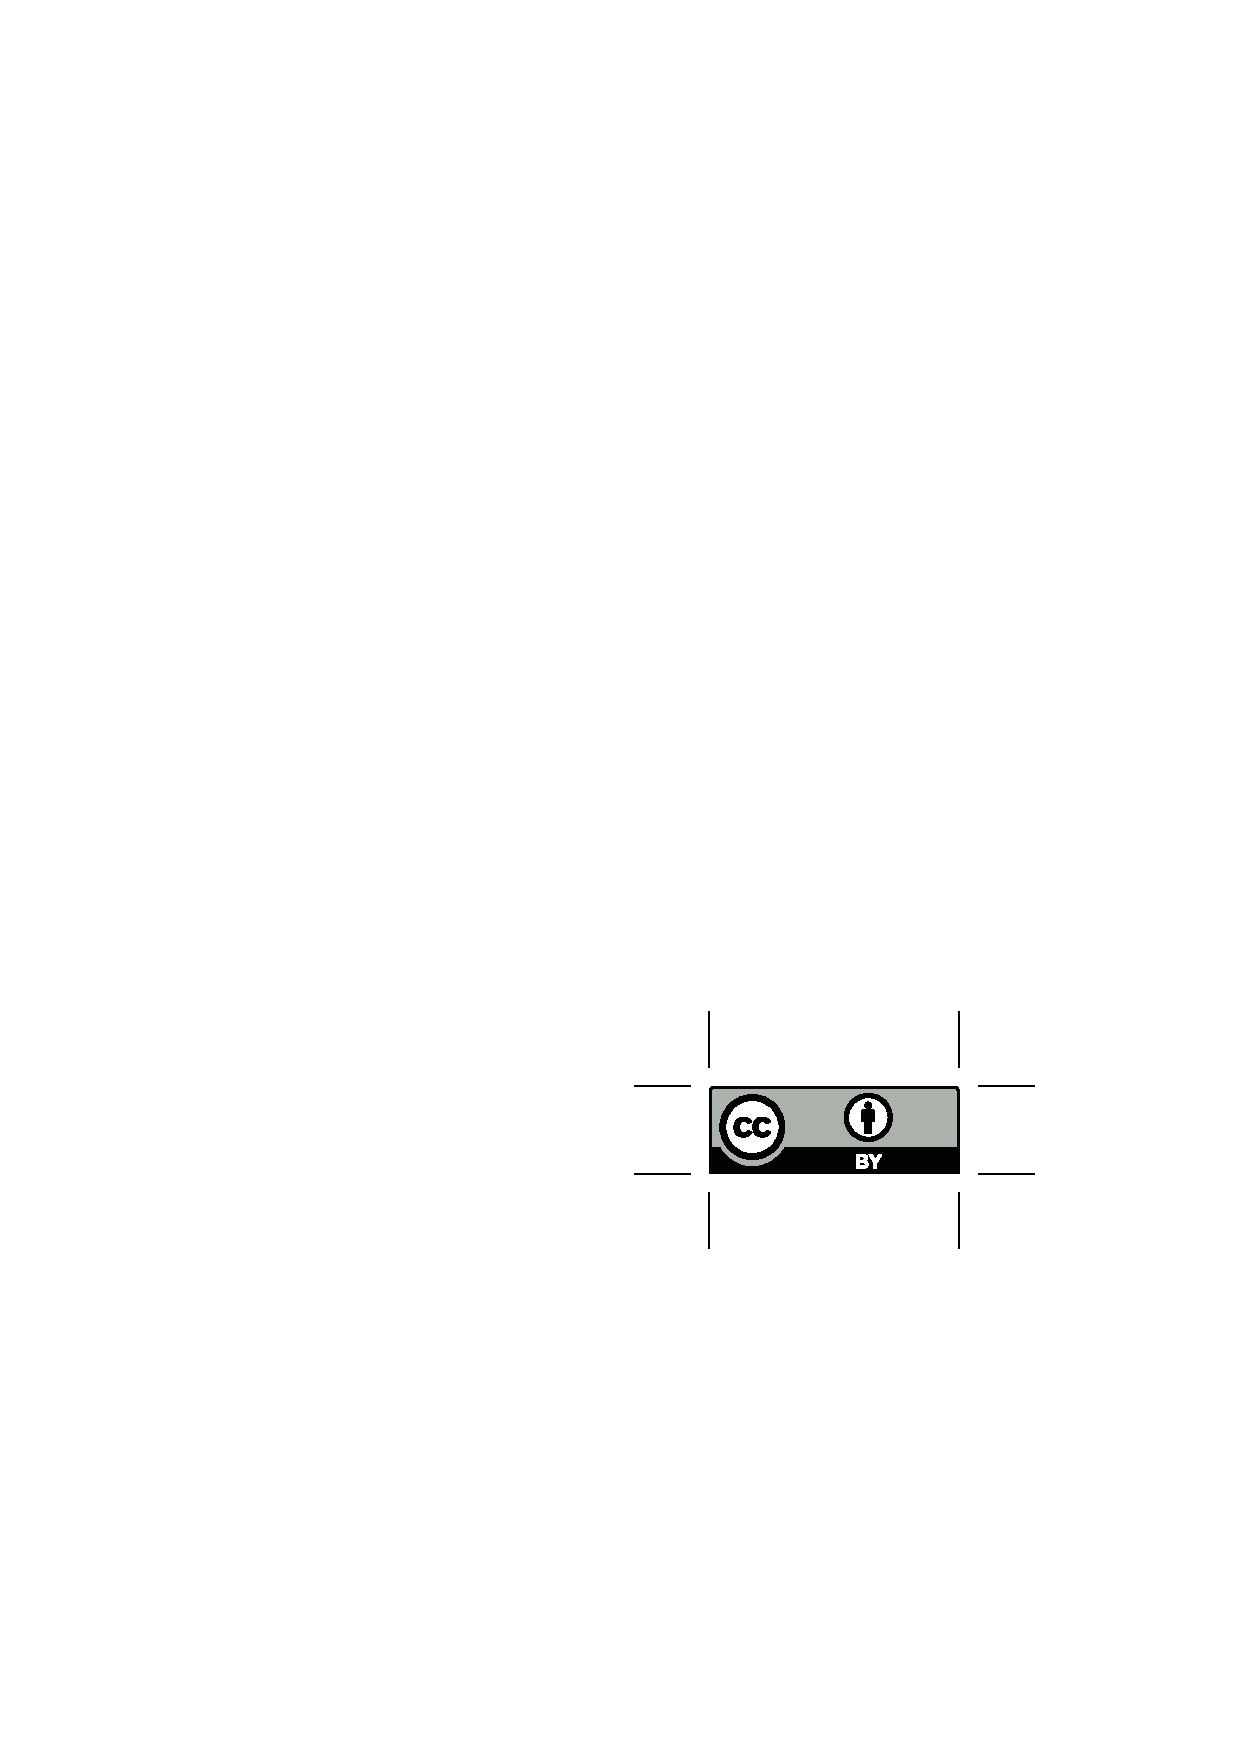
\includegraphics[width=0.90\textwidth]{by}}
  \end{minipage}\hfill
  \begin{minipage}{0.8\columnwidth}
   \href{https://creativecommons.org/licenses/by/4.0/}{This work is licensed under a Creative Commons Attribution International 4.0 License.}
  \end{minipage}
  \vspace{5pt}
}
\makeatother

\setcopyright{ifaamas}
\acmConference[AAMAS '25]{Proc.\@ of the 24th International Conference
on Autonomous Agents and Multiagent Systems (AAMAS 2025)}{May 19 -- 23, 2025}
{Detroit, Michigan, USA}{Y.~Vorobeychik, S.~Das, A.~Nowé  (eds.)}
\copyrightyear{2025}
\acmYear{2025}
\acmDOI{}
\acmPrice{}
\acmISBN{}

%%%%%%%%%%%%%%%%%%%%%%%%%%%%%%%%%%%%%%%%%%%%%%%%%%%%%%%%%%%%%%%%%%%%%%%%

%%% == IMPORTANT ==
%%% Use this command to specify your OpenReview submission number.
%%% In anonymous mode, it will be printed on the first page.

\acmSubmissionID{605}

%%% Use this command to specify the title of your paper.

\title[AAMAS-2025 MOISE+MARL]{An Organizationally-Oriented Approach to Enhancing Explainability and Control in Multi-Agent Reinforcement Learning}

% Add the subtitle below for an extended abstract
%\subtitle{Extended Abstract}

%%% Provide names, affiliations, and email addresses for all authors.

\author{Julien Soulé}
\affiliation{
  \institution{Univ. Grenoble Alpes}
  \city{Valence}
  \country{France}}
\email{julien.soule@lcis.grenoble-inp.fr}

\author{Jean-Paul Jamont}
\affiliation{
  \institution{Univ. Grenoble Alpes}
  \city{Valence}
  \country{France}}
\email{jean-paul.jamont@lcis.grenoble-inp.fr}

\author{Michel Occello}
\affiliation{
  \institution{Univ. Grenoble Alpes}
  \city{Valence}
  \country{France}}
\email{michel.occello@lcis.grenoble-inp.fr}

\author{Louis-Marie Traonouez}
\affiliation{
  \institution{Thales Land and Air Systems, BU IAS}
  \city{Rennes}
  \country{France}}
\email{louis-marie.traonouez@thalesgroup.com}

\author{Paul Théron}
\affiliation{
  \institution{AICA IWG}
  \city{La Guillermie}
  \country{France}}
\email{paul.theron@orange.fr}


%%% Use this environment to specify a short abstract for your paper.

\begin{abstract}
  Multi-Agent Reinforcement Learning can lead to the development of collaborative agent behaviors that show similarities with organizational concepts. Pushing forward this perspective, we introduce a novel framework that explicitly incorporates organizational roles and goals from the $\mathcal{M}OISE^+$ model into the MARL process, guiding agents to satisfy corresponding organizational constraints. By structuring training with roles and goals, we aim to enhance both the explainability and control of agent behaviors at the organizational level, whereas much of the literature primarily focuses on individual agents. Additionally, our framework includes a post-training analysis method to infer implicit roles and goals, offering insights into emergent agent behaviors. This framework has been applied across various MARL environments and algorithms, demonstrating coherence between predefined organizational specifications and those inferred from trained agents.
\end{abstract}

%%% The code below was generated by the tool at http://dl.acm.org/ccs.cfm.
%%% Please replace this example with code appropriate for your own paper.


%%% Use this command to specify a few keywords describing your work.
%%% Keywords should be separated by commas.

\keywords{Multi-Agent Reinforcement Learning; Organizational Explainability; Organizational Control}

%%%%%%%%%%%%%%%%%%%%%%%%%%%%%%%%%%%%%%%%%%%%%%%%%%%%%%%%%%%%%%%%%%%%%%%%

%%% Include any author-defined commands here.
         
\newcommand{\BibTeX}{\rm B\kern-.05em{\sc i\kern-.025em b}\kern-.08em\TeX}

%%%%%%%%%%%%%%%%%%%%%%%%%%%%%%%%%%%%%%%%%%%%%%%%%%%%%%%%%%%%%%%%%%%%%%%%

\begin{document}

%%% The following commands remove the headers in your paper. For final 
%%% papers, these will be inserted during the pagination process.

\pagestyle{fancy}
\fancyhead{}

%%% The next command prints the information defined in the preamble.

\maketitle 

%%%%%%%%%%%%%%%%%%%%%%%%%%%%%%%%%%%%%%%%%%%%%%%%%%%%%%%%%%%%%%%%%%%%%%%%



%%%%%%%%%%%%%%%%%%%%%%%%%%%%%%%%%%%%%%%%%%%%%%%%%%%%%%%%%%%%%%%%%%%%%%%%

%%% The acknowledgments section is defined using the "acks" environment
%%% (rather than an unnumbered section). The use of this environment 
%%% ensures the proper identification of the section in the article 
%%% metadata as well as the consistent spelling of the heading.


\section{Introduction}

% Context
Multi-Agent Reinforcement Learning (MARL) enables the discovery of a joint policy that controls agents' behaviors so they can achieve a global goal within a specific environment. 
This joint policy not only dictates the individual actions of agents but also manages their interactions with one another, and potentially with all other agents, without any preconceived notion of a predefined organization.

In environments that require social interaction among agents to optimally achieve the global goal, agents may converge in such a way that they exhibit recurring sets of similar behaviors across different testing episodes. 
These distinct sets of behaviors can demonstrate properties of specialization, complementarity, and stability, making them akin to implicit roles. Moreover, the trajectories of agents assuming these "implicit" roles may display similarities, such as recurrent observations at the end of each episode. These recurring patterns in agent histories can be interpreted as "implicit" goals, suggesting that agents may aim to pursue these as intermediate goals before reaching the global goal. These implicit roles and implicit goals form the foundation of an "implicit" structural and functional organization as defined in $\mathcal{M}OISE^+$~\cite{Hubner2007}.

However, it would be misleading to assume that all trained agents in any environment can be faithfully compared to a structural and functional organization. Indeed, we can interpret the behaviors of trained agents concerning their similarity to the potential vision of an implicit structural and functional organization, which we define as \textbf{organizational fit}.
While evaluating organizational fit would be useful to assess to what extent trained agents can naturally be explained as roles and goals, one could also consider the reverse approach. By guiding or encouraging agents to converge towards structural and functional organizations with higher organizational fit, we aim to enhance explainability and control in MARL.

\

% Problem
Building on these assumptions, this paper aims to further explore two key aspects:
\begin{enumerate*}[label={\roman*) },itemjoin={; \quad}]
    \item The \textbf{evaluation of organizational fit}, which seeks to measure how closely a joint policy aligns with a structural and functional organization. A significant challenge here is to understand under what conditions agents can be considered to form a structural and functional organization, given constraints imposed by the environment, goals, and other optional factors.
    Existing literature often addresses policy evaluation in terms of roles or goals~\cite{Isakov2024, Wen2024, Xie2024}, but these works generally lack a systematic and comprehensive approach. Current methods offer few clear tools for quantitatively and qualitatively measuring this organizational fit.
    \item The \textbf{control of organizational fit}, which aims to guide agents towards policies that conform to a structural and functional organization through user-defined constraints or incentives that implement roles and goals.
    The primary challenges include reducing the policy search space, improving convergence, and ensuring compliance with safety constraints.
    Existing approaches in this field often fall short in terms of enabling users to easily define and manage the application of organizational specifications in a practical manner within a standard MARL framework, without relying on paradigms such as Hierarchical Reinforcement Learning (HRL).
\end{enumerate*}

\

% Contribution
\noindent We introduce the \textbf{MOISE+MARL} framework, which integrates the Decentralized Partially Observable Markov Decision Process (Dec-POMDP) MARL framework with the $\mathcal{M}OISE^+$~\cite{Hubner2007} organizational model through proposed relationships. This framework allows users to manually define the logic of a role or a goal by relying on trajectory-based patterns to describe the expected behavior of an agent that has adopted a goal or mission. Once configured, they allow users to apply a role to an agent, adding constraints that automatically influence agents' policies by dynamically updating both the action space and reshaping the reward function. This framework also includes a method called \textbf{Trajectory-based Evaluation in MOISE+MARL} (TEMM), which uses unsupervised learning techniques to generalize implicit roles and implicit missions from observed trajectories across multiple test episodes. By measuring the gap between inferred implicit organizational specifications and actual behaviors, this method allows for a quantitative assessment of organizational fit. It is worth noting that unlike hierarchical reinforcement learning, which decomposes tasks into subtasks~\cite{Qi2024, Matsuyama2025, SaoMai2024}, our approach relies on explicit organizational roles and missions to guide agent coordination externally.

\

% Evaluation & Findings
We evaluated the MOISE+MARL framework in the following scenarios:
\begin{enumerate*}[label={\roman*) },itemjoin={; \quad}]
  \item Four distinct environments, each expected to result in the training of joint policies with different implicit organizations, to assess the generalizability of MOISE+ MARL's applicability
  \item Four MARL algorithms from the several families to assess their suitability with MOISE+ MARL during training and post-analysis
  \item Four sets of organizational specifications, one for each environment, to constrain agents in a manner that either enforces conformity intended for both manual and quantitative evaluation.
\end{enumerate*}

In all environments, we observed that agents having adopted roles do behave as expected according to their roles in a correlated way with a quantitative measure of the organizational fit by TEMM. The roles and missions inferred by TEMM closely align with the predefined specifications, demonstrating the internal consistency of MOISE+MARL, as the policy modifications introduced by organizational specifications are effectively captured by TEMM.
The results also indicate that policy-based and actor-critic algorithms are particularly well-suited for guiding agents towards stable policies. This stability allows agents to maintain consistent and coherent behaviors across episodes, which is essential for TEMM's generation of a stable implicit organization. In contrast, value-based algorithms showed greater variability in agent behaviors.

\

% Structure of the paper
\noindent The rest of the paper is organized as follows: \autoref{sec:related_works} presents works relative to evaluating and controlling organizational fit. \autoref{sec:moise_marl_framework} introduces the MOISE+MARL framework. \autoref{sec:TEMM_algorithm} describes the TEMM method. \autoref{sec:experimental_setup} describes the experimental protocol, particularly the environments and MARL algorithms. \autoref{sec:results} presents the experimental results. Finally, \autoref{sec:discussion_conclusion_future_work} discusses and concludes on the evaluation and control of organizational fit.


\section{Related works}
\label{sec:related_works}

This section explores works related to organizational fit, as framed by the two core issues introduced.

\subsection{Evaluating organizational fit}

Some works may be related to role or goal inference regarding the need to compute organizational fit or close concepts.
%
Wilson et al.~\cite{wilson2008learning} develop a method for transferring roles in Multi-Agent MDPs, which helps agents adapt by transferring roles across different environments. However, their model lacks the role abstraction as it focuses on specific, task-related roles.
%
Berenji and Vengerov~\cite{berenji2000learning} investigate coordination and role inference in UAV missions, enhancing cooperation through modeling agent dependencies. While useful for cooperation, their approach remains task-specific and does not provide the implicit role computation needed for organizational fit.
%
Yusuf and Baber~\cite{yusuf2020inferential} use inferential reasoning and Bayesian methods to facilitate task coordination among diverse agents. Though effective in dynamic coordination, their framework lacks role abstraction and does not measure alignment with an broader organizational structure either.
%
Serrino et al.~\cite{serrino2019finding} examine dynamic role inference in social settings, where agents deduce roles through interactions. While they enable flexible role understanding, their approach focuses on immediate operational roles rather than implicit roles that align with organizational models.

While some works explore organizational concepts in MARL, none explicitly address the computation of organizational alignment as we define it. Our concept of organizational fit requires a framework that assesses alignment with implicit goals.


\subsection{Controlling organizational fit}
Controlling organizational fit involves aligning the agents' policies with a predefined organization, often using constraints or incentives.
%
Achiam et al.~\cite{achiam2017cpo} introduce CPO, adjusting policies with safety constraints while maximizing rewards. MOISE+MARL, however, introduces constraints beyond safety to shape behavior toward organizational expectations by externally guiding agent learning.
%
Ray et al.~\cite{ray2019benchmarking} use Lagrange multipliers to integrate constraints into the reward function, balancing reward and constraint adherence. MOISE+MARL extends this by dynamically modifying the action space to enforce constraint adherence at various levels, offering flexible control over agent behaviors.
%
Safe exploration ensures agents learn while adhering to safety constraints. Garcia et al.~\cite{garcia2015comprehensive} overview methods for maintaining safe exploration, and Alshiekh et al.~\cite{alshiekh2018safe} propose shielding to block unsafe actions. MOISE+MARL goes further by using constraints to guide agents toward behaviors that align with organizational roles.
%
HRL breaks tasks into subtasks, aligning with organizational hierarchies. Ghavamzadeh et al.~\cite{ghavamzadeh2006hrl} illustrate that HRL can improve coordination. MOISE+MARL constrains MARL externally, offering a modular granularity and generating refined behaviors under organizational constraints.
%
Controlling Communication and Coordination is essential for ensuring organizational fit, especially in large-scale systems. Foerster et al.~\cite{foerster2018communication} propose decentralized coordination through shared knowledge, allowing agents to operate without centralized control.

Unlike HRL, the MOISE+MARL framework stands out for incorporating external organizational constraints that influence agents within a standard MARL framework, enabling modular granularity. Unlike Shielding or CPO, which typically focus on safety constraints, MOISE+MARL goes further by relying on actions and reward modifications to align with roles. % MOISE+MARL aims to handles scalability and adaptability by simplifying users interactions to defining and applying a smaller amount of organizational specifications.


\section{The MOISE+MARL framework}
\label{sec:moise_marl_framework}

This section introduces the formalism used to describe the functioning framework of the MOISE+MARL framework.

\subsection{Markov framework for MARL}

To apply MARL techniques, we rely on the \textit{Decentralized Partially Observable Markov Decision Process} (Dec-POMDP) \cite{Oliehoek2016}. Dec-POMDPs naturally model decentralized multi-agent coordination under partial observability, making them well suited for integrating organizational constraints. Unlike \textit{Partially Observable Stochastic Games} (POSG), the Dec-POMDP allows for a common reward function for agents, which promotes collaboration~\cite{Beynier2013}.

A Dec-POMDP $d \in D$ (where $D$ is the set of Dec-POMDPs) is defined as a 7-tuple $d = \langle S, \{A_i\}, T, R, \{\Omega_i\}, O, \gamma \rangle$, where $S = \{s_1,\dots,s_{|S|}\}$ is the set of possible states; $A_{i} = \{a_{1}^{i},\dots,a_{|A_{i}|}^{i}\}$ is the set of possible actions for agent $i$; $T$ represents the set of transition probabilities, with $T(s,a,s') = \probP(s'|s,a)$ as the probability of transitioning from state $s$ to state $s'$ following action $a$; $R: S \times A \times S \rightarrow \mathbb{R}$ is the reward function, assigning a reward based on the initial state, the action taken, and the resulting state; $\Omega_{i} = \{o_{1}^{i},\dots,o_{|\Omega_{i}|}^{i}\}$ is the set of possible observations for agent $i$; $O$ represents the set of observation probabilities, where $O(s',a,o) = \probP(o|s',a)$ is the probability of obtaining observation $o$ after performing action $a$ and reaching state $s'$; and $\gamma \in [0,1]$ is the discount factor
%, used to weight future rewards.

The following formalism is used with MOISE+MARL to solve the Dec-POMDP~\cite{Beynier2013,Albrecht2024}: $\mathcal{A}$ represents the set of $n$ \textbf{agents}; $\Pi$ denotes the set of \textbf{policies}, where a policy $\pi \in \Pi, \pi: \Omega \rightarrow A$ deterministically maps an observation to an action, representing the agent's internal strategy; $\Pi_{joint}$ represents the set of \textbf{joint policies}, with a joint policy $\pi_{joint} \in \Pi_{joint}, \pi_{joint}: \Omega^n \rightarrow A^n = \Pi^n$, which selects an action for each agent based on their respective observations, acting as a collection of policies used by agents within a team; $H$ is the set of \textbf{histories}, where a history (or trajectory) over $z \in \mathbb{N}$ steps (typically the maximum number of steps in an episode) is represented as the $z$-tuple $h = \langle \langle \omega_{k}, a_{k}\rangle | k \leq z, \omega \in \Omega, a \in A\rangle$, capturing successive observations and actions; $H_{joint}$ stands for the set of \textbf{joint histories}, with a joint history $h_{joint} \in H_{joint}$ over $z$ steps defined as the set of agent histories: $h_{joint} = \{h_1, h_2, \dots, h_n\}$; and finally, $V_{joint}(\pi_{joint}): \Pi_{joint} \rightarrow \mathbb{R}$ denotes the \textbf{expected cumulative reward} over a finite horizon (assuming $\gamma < 1$ or if the number of steps in an episode is finite), where $\pi_{joint}$ represents the joint policy for team $i$, with $\pi_{joint,-i}$ being the joint policies of other teams, considered as fixed.


% We refer to \textbf{solving the Dec-POMDP} as the search for a joint policy $\pi_{joint} \in \Pi_{joint}$ such that $\pi_{joint}s)$, achieving at least an expected cumulative reward of $s$, where $s \in \mathbb{R}$.

\subsection{The $\mathcal{M}OISE^+$ organizational model}

\begin{figure}[h!]
    


\tikzset{every picture/.style={line width=0.75pt}} %set default line width to 0.75pt        

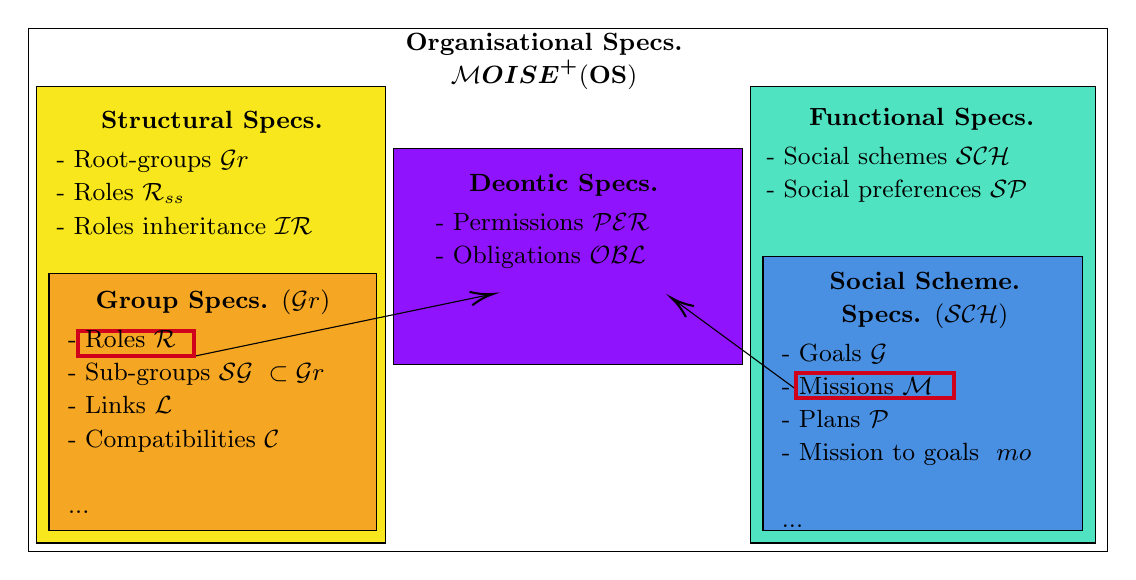
\begin{tikzpicture}[x=0.75pt,y=0.75pt,yscale=-1,xscale=1]
%uncomment if require: \path (0,1656); %set diagram left start at 0, and has height of 1656

%Shape: Rectangle [id:dp6756844921493015] 
\draw  [fill={rgb, 255:red, 248; green, 231; blue, 28 }  ,fill opacity=1 ] (46,1204) -- (214,1204) -- (214,1424) -- (46,1424) -- cycle ;
%Shape: Rectangle [id:dp3759944257810566] 
\draw  [fill={rgb, 255:red, 80; green, 227; blue, 194 }  ,fill opacity=1 ] (390,1204) -- (556,1204) -- (556,1424) -- (390,1424) -- cycle ;
%Shape: Rectangle [id:dp28244406216006945] 
\draw  [fill={rgb, 255:red, 144; green, 19; blue, 254 }  ,fill opacity=1 ] (218,1234) -- (386,1234) -- (386,1338) -- (218,1338) -- cycle ;
%Shape: Rectangle [id:dp32232123359581766] 
\draw   (42,1176) -- (562,1176) -- (562,1428) -- (42,1428) -- cycle ;
%Shape: Rectangle [id:dp7605706269262755] 
\draw  [fill={rgb, 255:red, 74; green, 144; blue, 226 }  ,fill opacity=1 ] (396,1286) -- (550,1286) -- (550,1418) -- (396,1418) -- cycle ;
%Shape: Rectangle [id:dp33110985390647496] 
\draw   (52,1294) -- (210,1294) -- (210,1418) -- (52,1418) -- cycle ;
%Shape: Rectangle [id:dp8653560038381976] 
\draw  [fill={rgb, 255:red, 245; green, 166; blue, 35 }  ,fill opacity=1 ] (52,1294) -- (210,1294) -- (210,1418) -- (52,1418) -- cycle ;
%Straight Lines [id:da09781093164567278] 
\draw    (412,1350) -- (353.61,1307.18) ;
\draw [shift={(352,1306)}, rotate = 36.25] [color={rgb, 255:red, 0; green, 0; blue, 0 }  ][line width=0.75]    (10.93,-3.29) .. controls (6.95,-1.4) and (3.31,-0.3) .. (0,0) .. controls (3.31,0.3) and (6.95,1.4) .. (10.93,3.29)   ;
%Straight Lines [id:da3938396723807833] 
\draw    (122,1334) -- (264.04,1304.41) ;
\draw [shift={(266,1304)}, rotate = 168.23] [color={rgb, 255:red, 0; green, 0; blue, 0 }  ][line width=0.75]    (10.93,-3.29) .. controls (6.95,-1.4) and (3.31,-0.3) .. (0,0) .. controls (3.31,0.3) and (6.95,1.4) .. (10.93,3.29)   ;
%Shape: Rectangle [id:dp269311335478327] 
\draw  [color={rgb, 255:red, 208; green, 2; blue, 27 }  ,draw opacity=1 ][line width=1.5]  (66,1322) -- (122,1322) -- (122,1334) -- (66,1334) -- cycle ;
%Shape: Rectangle [id:dp7449860119164387] 
\draw  [color={rgb, 255:red, 208; green, 2; blue, 27 }  ,draw opacity=1 ][line width=1.5]  (412,1342) -- (488,1342) -- (488,1354) -- (412,1354) -- cycle ;


% Text Node
\draw (472.5,1237.41) node   [align=left] {\begin{minipage}[lt]{112.2pt}\setlength\topsep{0pt}
\begin{center}
\textbf{{\small Functional Specs.}}
\end{center}
{\small  - Social schemes $\displaystyle \mathcal{SCH}$}\\{\small  - Social preferences $\displaystyle \mathcal{SP}$}
\end{minipage}};
% Text Node
\draw (474,1355) node   [align=left] {\begin{minipage}[lt]{103.36pt}\setlength\topsep{0pt}
\begin{center}
\textbf{{\small Social Scheme.}}\\{\small \textbf{Specs. }$\displaystyle (\mathcal{SCH})$}
\end{center}
{\small  - Goals $\displaystyle \mathcal{G}$}\\{\small  - Missions $\displaystyle \mathcal{M}$}\\{\small  - Plans $\displaystyle \mathcal{P}$}\\{\small  - Mission to goals \ $\displaystyle mo$}\\\\{\small  ...}
\end{minipage}};
% Text Node
\draw (131,1356) node   [align=left] {\begin{minipage}[lt]{104.72pt}\setlength\topsep{0pt}
\begin{center}
{\small \textbf{Group Specs. }$\displaystyle (\mathcal{G} r)$}
\end{center}
{\small  - Roles $\displaystyle \mathcal{R}$}\\{\small  - Sub-groups $\displaystyle \mathcal{SG} \ \subset \mathcal{G} r$}\\{\small  - Links $\displaystyle \mathcal{L}$}\\{\small  - Compatibilities $\displaystyle \mathcal{C}$}\\\\{\small  ...}
\end{minipage}};
% Text Node
\draw (181,1177) node [anchor=north west][inner sep=0.75pt]   [align=left] {\begin{minipage}[lt]{162.41pt}\setlength\topsep{0pt}
\begin{center}
{\small \textbf{Organisational Specs. }$\displaystyle \mathcal{M}\boldsymbol{OISE^{+}}$($\displaystyle \mathbf{OS}$)}
\end{center}

\end{minipage}};
% Text Node
\draw (300,1269.09) node   [align=left] {\begin{minipage}[lt]{92.48pt}\setlength\topsep{0pt}
\begin{center}
\textbf{{\small Deontic Specs.}}
\end{center}
{\small  - Permissions $\displaystyle \mathcal{PER}$}\\{\small  - Obligations $\displaystyle \mathcal{OBL}$}
\end{minipage}};
% Text Node
\draw (130.5,1245.69) node   [align=left] {\begin{minipage}[lt]{112.2pt}\setlength\topsep{0pt}
\begin{center}
\textbf{{\small Structural Specs.}}
\end{center}
{\small  - Root-groups $\displaystyle \mathcal{G} r$}\\{\small  - Roles $\displaystyle \mathcal{R}_{ss}$}\\{\small  - Roles inheritance $\displaystyle \mathcal{IR}$}
\end{minipage}};


\end{tikzpicture}
    \caption{A synthetic view of the $\mathcal{M}OISE^+$ model}
    \label{fig:moise_model}
\end{figure}

As illustrated in \autoref{fig:moise_model}, $\mathcal{M}OISE^+$ comprises three types of organizational specifications:

\noindent \paragraph{\textbf{Structural Specifications (SS)}} define how agents are structured, expressed as $\mathcal{SS} = \langle \mathcal{R}, \mathcal{IR}, \mathcal{G} \rangle$. $\mathcal{R}_{ss}$ is the set of roles ($\rho \in \mathcal{R}$) with an inheritance relation $\mathcal{IR}$ where $\rho_1 \sqsubset \rho_2$ if $\rho_1$ inherits from $\rho_2$. $\mathcal{GR}$ includes groups $\langle \mathcal{R}, \mathcal{SG}, \mathcal{L}^{intra}, \mathcal{L}^{inter}, \allowbreak \mathcal{C}^{intra}, \mathcal{C}^{inter}, np, ng \rangle$. Links ($\mathcal{L}$) define connections between roles: acquaintance, communication, or authority. Compatibilities $\mathcal{C}$ denote roles that agents can play together. Intra- and inter-group links and compatibilities are shown by $\mathcal{L}^{intra}$, $\mathcal{L}^{inter}$, $\mathcal{C}^{intra}$, and $\mathcal{C}^{inter}$, with $np$ and $ng$ defining role and subgroup counts.

\noindent \paragraph{\textbf{Functional Specifications (FS)}} describe the agents' goals, represented as $\mathcal{FS} = \langle \mathcal{SCH}, \mathcal{PO} \rangle$. The social scheme $\mathcal{SCH}$ includes global goals $\mathcal{G}$, missions $\mathcal{M}$, and plans $\mathcal{P}$ that organize goals in a tree structure. Plans link goals with an operator ($op$) indicating sequence, choice, or parallel completion. Missions map to goal sets ($mo$), and agent counts per mission are specified by $nm$. Preferences $\mathcal{PO}$ indicate which missions agents prefer, denoted as $m_1 \prec m_2$.

\noindent \paragraph{\textbf{Deontic Specifications (DS)}} indicate the relationship between roles goals, given by $\mathcal{DS} = \langle \mathcal{OBL}, \mathcal{PER} \rangle$. Time constraints $\mathcal{TC}$ set periods for permissions or obligations ($Any$ for any time). Obligations ($\mathcal{OBL}$) require agents in role $\rho_a$ to undertake mission $m$ at times $tc$, while permissions ($\mathcal{PER}$) allow it. The $rds$ function maps roles to their deontic specifications as $\langle tc, y, m \rangle$ where $y$ distinguishes permission (0) from obligation (1).

\

\noindent Organizational specifications applied to agents are roles and goals (as missions) through permissions or obligations. Indeed, the other structural specifications such as compatibilities or links are inherent to roles. Similarly, we consider that the goals, the missions, and their mapping ($mo$) are enough to also link all of the other functional specifications such as plans, cardinalities, or preference orders.
Consequently, we consider it is sufficient to take into account roles, missions (goal and mapping) and permissions/obligations when linking $\mathcal{M}OISE^+$ with Dec-POMDP. 

\begin{figure*}[t]
    \label{eq:single_value_function}
    \raggedright
    \textbf{\textit{Definition 1} \quad Sate-Value function adapted to constraint guides in AEC mode:}
    \begin{gather*}
      \text{\quad \quad} V^{\pi^j}(s_t) = \hspace{-0.75cm} \sum_{\textcolor{red}{ \substack{a_{t} \in A \text{ if } rn() < ch_{t}, \\ 
      a_{t} \in A_{t} \text{ else}}
      }}{\hspace{-0.7cm} \pi_i(a_{t} | \omega_t)} \sum_{s_{t+1} \in S}{\hspace{-0.1cm} T(s_{t+1} | s_t, a_{t})[R(s_t,a_{t},s_{t+1}) + \hspace{-0.1cm} \textcolor{blue}{ \sum_{m \in \mathcal{M}_i}{ \hspace{-0.1cm} v_m(t) \frac{grg_m(h_{t+1})}{1 - p + \epsilon} } } + \textcolor{red}{(1-ch_t) \times rrg(\omega_t,a_{t+1})} + V^{\pi^j_{i+1 \ mod \ n}}(s_{t+1})]}
    \end{gather*}  
    %
    \textcolor{red}{\[\text{With } rag(h_t, \omega_t) = A_{t} \times \mathbb{R} \text{, } \langle a_t, ch_{t} \rangle \in A_{t} \times \mathbb{R} \text{ ; } \text{ and } rn: \emptyset \to [0,1[ \text{, a uniform random function}\]}
    %
    \vspace{-0.5cm}
    \textcolor{blue}{
    \begin{gather*}
    \text{With } \omega_t = O(\omega_t | s_t, a_t) \text{ ; } h_t = \{h_0 = \langle \rangle, h_{t+1} = \langle h_t, \langle \omega_{t+1}, a_{t+1} \rangle \rangle \} \text{ ; } grg_m(h) = \hspace{-0.8cm} \sum_{(grg_i,w_i) \in mo(m)}{\hspace{-0.8cm} w_i \times grg_i(h)} \text{ ; } \epsilon \in \mathbb{R}_{>0} \text{ ; }
    \end{gather*}
    }
    \vspace{-0.75cm}
    \textcolor{blue}{
    \begin{gather*}
    v_m(t) = \{ 1 \text{ if } t \in t_c \text{ ; else } 0 \} \text{ ; } \text{ and } \mathcal{M}_i = \{m_j | \langle ar(i),m_j,t_c,p \rangle \in \mathcal{M}\}
    \end{gather*}
    }
    \vspace{-0.6cm}
\end{figure*}

\subsection{Linking $\mathcal{M}OISE^+$ with MARL}

\begin{figure}[h!]
    \centering
    \tikzset{every picture/.style={line width=0.75pt}} %set default line width to 0.75pt        

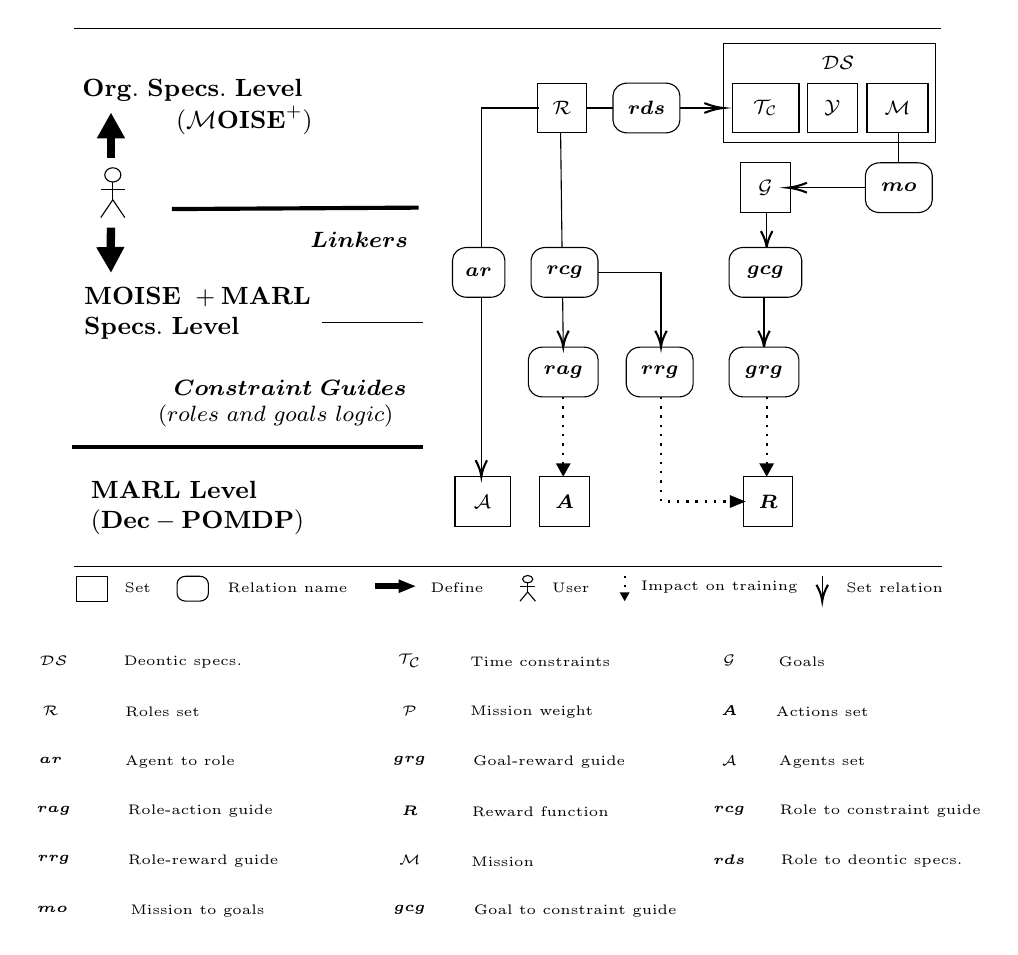
\begin{tikzpicture}[x=0.75pt,y=0.75pt,yscale=-1.2,xscale=1.4]
    %uncomment if require: \path (0,2584); %set diagram left start at 0, and has height of 2584

    %Straight Lines [id:da4973066741986565] 
    \draw [line width=1.5]    (118.21,2302.58) -- (203.1,2302) ;
    %Straight Lines [id:da14807114776731778] 
    \draw    (368.35,2272) -- (368.35,2294) -- (332.16,2294) ;
    \draw [shift={(330.16,2294)}, rotate = 360] [color={rgb, 255:red, 0; green, 0; blue, 0 }  ][line width=0.75]    (6.56,-1.97) .. controls (4.17,-0.84) and (1.99,-0.18) .. (0,0) .. controls (1.99,0.18) and (4.17,0.84) .. (6.56,1.97)   ;
    %Straight Lines [id:da16285043353898754] 
    \draw [line width=1.5]    (83.88,2398) -- (204.61,2398) ;
    %Straight Lines [id:da6299512000169913] 
    \draw    (169.94,2348) -- (204.61,2348) ;
    %Straight Lines [id:da64750232417664] 
    \draw    (84.65,2446) -- (383.15,2446) ;
    %Straight Lines [id:da35895220906699743] 
    \draw    (84.65,2230) -- (383,2230) ;
    %Straight Lines [id:da715014372569708] 
    \draw    (244.68,2262) -- (224.68,2262) -- (224.68,2408) ;
    \draw [shift={(224.68,2410)}, rotate = 270] [color={rgb, 255:red, 0; green, 0; blue, 0 }  ][line width=0.75]    (6.56,-1.97) .. controls (4.17,-0.84) and (1.99,-0.18) .. (0,0) .. controls (1.99,0.18) and (4.17,0.84) .. (6.56,1.97)   ;
    %Straight Lines [id:da71870438525014] 
    \draw    (251.96,2328) -- (286.51,2328) -- (286.51,2356) ;
    \draw [shift={(286.51,2358)}, rotate = 270] [color={rgb, 255:red, 0; green, 0; blue, 0 }  ][line width=0.75]    (6.56,-1.97) .. controls (4.17,-0.84) and (1.99,-0.18) .. (0,0) .. controls (1.99,0.18) and (4.17,0.84) .. (6.56,1.97)   ;
    %Straight Lines [id:da6006267784187092] 
    \draw [line width=0.75]  [dash pattern={on 0.84pt off 2.51pt}]  (252.87,2378) -- (252.87,2407) ;
    \draw [shift={(252.87,2410)}, rotate = 270] [fill={rgb, 255:red, 0; green, 0; blue, 0 }  ][line width=0.08]  [draw opacity=0] (5.36,-2.57) -- (0,0) -- (5.36,2.57) -- cycle    ;
    %Straight Lines [id:da8743336135156266] 
    \draw    (322.88,2304) -- (322.88,2316) ;
    \draw [shift={(322.88,2318)}, rotate = 270] [color={rgb, 255:red, 0; green, 0; blue, 0 }  ][line width=0.75]    (6.56,-1.97) .. controls (4.17,-0.84) and (1.99,-0.18) .. (0,0) .. controls (1.99,0.18) and (4.17,0.84) .. (6.56,1.97)   ;
    %Straight Lines [id:da14641229967966152] 
    \draw [line width=0.75]  [dash pattern={on 0.84pt off 2.51pt}]  (322.88,2378) -- (322.88,2407) ;
    \draw [shift={(322.88,2410)}, rotate = 270] [fill={rgb, 255:red, 0; green, 0; blue, 0 }  ][line width=0.08]  [draw opacity=0] (5.36,-2.57) -- (0,0) -- (5.36,2.57) -- cycle    ;
    %Straight Lines [id:da9260929933425808] 
    \draw [line width=0.75]  [dash pattern={on 0.84pt off 2.51pt}]  (286.51,2378) -- (286.51,2420) -- (312.61,2420) ;
    \draw [shift={(315.61,2420)}, rotate = 180] [fill={rgb, 255:red, 0; green, 0; blue, 0 }  ][line width=0.08]  [draw opacity=0] (5.36,-2.57) -- (0,0) -- (5.36,2.57) -- cycle    ;
    %Straight Lines [id:da3057006030233673] 
    \draw [line width=0.75]  [dash pattern={on 0.84pt off 2.51pt}]  (274,2449.7) -- (274,2457) ;
    \draw [shift={(274,2460)}, rotate = 270] [fill={rgb, 255:red, 0; green, 0; blue, 0 }  ][line width=0.08]  [draw opacity=0] (3.57,-1.72) -- (0,0) -- (3.57,1.72) -- cycle    ;
    %Straight Lines [id:da07288166228322246] 
    \draw    (342,2449.98) -- (342,2458) ;
    \draw [shift={(342,2460)}, rotate = 270] [color={rgb, 255:red, 0; green, 0; blue, 0 }  ][line width=0.75]    (6.56,-1.97) .. controls (4.17,-0.84) and (1.99,-0.18) .. (0,0) .. controls (1.99,0.18) and (4.17,0.84) .. (6.56,1.97)   ;
    %Shape: Ellipse [id:dp8508274348425935] 
    \draw   (95.09,2288.86) .. controls (95.09,2287.28) and (96.33,2286) .. (97.85,2286) .. controls (99.38,2286) and (100.62,2287.28) .. (100.62,2288.86) .. controls (100.62,2290.44) and (99.38,2291.71) .. (97.85,2291.71) .. controls (96.33,2291.71) and (95.09,2290.44) .. (95.09,2288.86) -- cycle ;
    %Straight Lines [id:da3825450168053828] 
    \draw    (97.85,2291.71) -- (97.85,2298.86) ;
    %Straight Lines [id:da521321206042058] 
    \draw    (97.85,2298.86) -- (93.71,2306) ;
    %Straight Lines [id:da055514206493922025] 
    \draw    (97.85,2298.86) -- (102,2306) ;
    %Straight Lines [id:da8996496708356774] 
    \draw    (102,2294.57) -- (93.71,2294.57) ;

    %Straight Lines [id:da31678488015771755] 
    \draw [line width=2.25]    (188,2454) -- (196.97,2454) ;
    \draw [shift={(201.97,2454)}, rotate = 180] [fill={rgb, 255:red, 0; green, 0; blue, 0 }  ][line width=0.08]  [draw opacity=0] (5.72,-2.75) -- (0,0) -- (5.72,2.75) -- cycle    ;
    %Shape: Ellipse [id:dp3927356466672782] 
    \draw   (238.88,2451.17) .. controls (238.88,2450.36) and (239.67,2449.7) .. (240.64,2449.7) .. controls (241.61,2449.7) and (242.4,2450.36) .. (242.4,2451.17) .. controls (242.4,2451.99) and (241.61,2452.65) .. (240.64,2452.65) .. controls (239.67,2452.65) and (238.88,2451.99) .. (238.88,2451.17) -- cycle ;
    %Straight Lines [id:da3365602555559104] 
    \draw    (240.64,2452.65) -- (240.64,2456.32) ;
    %Straight Lines [id:da7990875235744026] 
    \draw    (240.64,2456.32) -- (238,2460) ;
    %Straight Lines [id:da23945649338821617] 
    \draw    (240.64,2456.32) -- (243.28,2460) ;
    %Straight Lines [id:da11927353559661591] 
    \draw    (243.28,2454.12) -- (238,2454.12) ;

    %Straight Lines [id:da5816423191130675] 
    \draw    (251.96,2272) -- (252.85,2356) ;
    \draw [shift={(252.87,2358)}, rotate = 269.39] [color={rgb, 255:red, 0; green, 0; blue, 0 }  ][line width=0.75]    (6.56,-1.97) .. controls (4.17,-0.84) and (1.99,-0.18) .. (0,0) .. controls (1.99,0.18) and (4.17,0.84) .. (6.56,1.97)   ;
    %Straight Lines [id:da9310455126832857] 
    \draw    (321.97,2338) -- (321.97,2356) ;
    \draw [shift={(321.97,2358)}, rotate = 270] [color={rgb, 255:red, 0; green, 0; blue, 0 }  ][line width=0.75]    (6.56,-1.97) .. controls (4.17,-0.84) and (1.99,-0.18) .. (0,0) .. controls (1.99,0.18) and (4.17,0.84) .. (6.56,1.97)   ;
    %Shape: Rectangle [id:dp293492578719597] 
    \draw   (120,2453) .. controls (120,2451.34) and (121.34,2450) .. (123,2450) -- (127.72,2450) .. controls (129.37,2450) and (130.72,2451.34) .. (130.72,2453) -- (130.72,2457) .. controls (130.72,2458.66) and (129.37,2460) .. (127.72,2460) -- (123,2460) .. controls (121.34,2460) and (120,2458.66) .. (120,2457) -- cycle ;
    %Straight Lines [id:da33566712615128225] 
    \draw    (261.05,2262) -- (306,2262) ;
    \draw [shift={(308,2262)}, rotate = 180] [color={rgb, 255:red, 0; green, 0; blue, 0 }  ][line width=0.75]    (6.56,-1.97) .. controls (4.17,-0.84) and (1.99,-0.18) .. (0,0) .. controls (1.99,0.18) and (4.17,0.84) .. (6.56,1.97)   ;
    %Shape: Rectangle [id:dp28383270948937667] 
    \draw   (308,2236) -- (381.08,2236) -- (381.08,2276) -- (308,2276) -- cycle ;
    %Straight Lines [id:da18020989903965012] 
    \draw [line width=3]    (97.22,2282) -- (97.22,2270) ;
    \draw [shift={(97.22,2264)}, rotate = 90] [fill={rgb, 255:red, 0; green, 0; blue, 0 }  ][line width=0.08]  [draw opacity=0] (10.18,-4.89) -- (0,0) -- (10.18,4.89) -- cycle    ;
    %Straight Lines [id:da018421338049046554] 
    \draw [line width=3]    (97.22,2310) -- (97.11,2322.37) ;
    \draw [shift={(97.22,2328)}, rotate = 268.86] [fill={rgb, 255:red, 0; green, 0; blue, 0 }  ][line width=0.08]  [draw opacity=0] (10.18,-4.89) -- (0,0) -- (10.18,4.89) -- cycle    ;
    %Shape: Rectangle [id:dp7281037051878541] 
    \draw   (85.42,2450) -- (96.13,2450) -- (96.13,2460) -- (85.42,2460) -- cycle ;

    % Text Node
    \draw (362,2544.5) node  [font=\tiny] [align=left] {Role to constraint guide};
    % Text Node
    \draw (342,2524.5) node  [font=\tiny] [align=left] {Agents set};
    % Text Node
    \draw (342,2504.5) node  [font=\tiny] [align=left] {Actions set};
    % Text Node
    \draw (257,2584.5) node  [font=\tiny] [align=left] {Goal to constraint guide};
    % Text Node
    \draw (335,2484.5) node  [font=\tiny] [align=left] {Goals};
    % Text Node
    \draw (359,2564.5) node  [font=\tiny] [align=left] {Role to deontic specs.};
    % Text Node
    \draw (232,2564.5) node  [font=\tiny] [align=left] {Mission};
    % Text Node
    \draw (245,2544.5) node  [font=\tiny] [align=left] {Reward function};
    % Text Node
    \draw (248,2524.5) node  [font=\tiny] [align=left] {Goal-reward guide};
    % Text Node
    \draw (242,2504.5) node  [font=\tiny] [align=left] {Mission weight};
    % Text Node
    \draw (245,2484.5) node  [font=\tiny] [align=left] {Time constraints};
    % Text Node
    \draw (127,2584.5) node  [font=\tiny] [align=left] {Mission to goals};
    % Text Node
    \draw (129,2564.5) node  [font=\tiny] [align=left] {Role-reward guide};
    % Text Node
    \draw (128,2544.5) node  [font=\tiny] [align=left] {Role-action guide};
    % Text Node
    \draw (121,2524.5) node  [font=\tiny] [align=left] {Agent to role};
    % Text Node
    \draw (115,2504.5) node  [font=\tiny] [align=left] {Roles set};
    % Text Node
    \draw (122,2484.5) node  [font=\tiny] [align=left] {Deontic specs.};
    % Text Node
    \draw (310,2544) node  [font=\tiny] [align=left] {$\displaystyle \boldsymbol{rcg}$};
    % Text Node
    \draw (200,2504) node  [font=\tiny] [align=left] {$\displaystyle \mathcal{P}$};
    % Text Node
    \draw (200,2484) node  [font=\tiny] [align=left] {$\displaystyle \mathcal{T_{C}}$};
    % Text Node
    \draw (200,2564) node  [font=\tiny] [align=left] {$\displaystyle \mathcal{M}$};
    % Text Node
    \draw (77.5,2484) node  [font=\tiny] [align=left] {$\displaystyle \mathcal{DS}$};
    % Text Node
    \draw (310,2564) node  [font=\tiny] [align=left] {$\displaystyle \boldsymbol{rds}$};
    % Text Node
    \draw (310,2504) node  [font=\tiny] [align=left] {$\displaystyle \boldsymbol{A}$};
    % Text Node
    \draw (200,2544) node  [font=\tiny] [align=left] {$\displaystyle \boldsymbol{R}$};
    % Text Node
    \draw (310,2524) node  [font=\tiny] [align=left] {$\displaystyle \mathcal{A}$};
    % Text Node
    \draw (200,2524) node  [font=\tiny] [align=left] {$\displaystyle \boldsymbol{grg}$};
    % Text Node
    \draw (77.5,2564) node  [font=\tiny] [align=left] {$\displaystyle \boldsymbol{rrg}$};
    % Text Node
    \draw (77.5,2544) node  [font=\tiny] [align=left] {$\displaystyle \boldsymbol{rag}$};
    % Text Node
    \draw (200,2584) node  [font=\tiny] [align=left] {$\displaystyle \boldsymbol{gcg}$};
    % Text Node
    \draw (76.5,2524) node  [font=\tiny] [align=left] {$\displaystyle \boldsymbol{ar}$};
    % Text Node
    \draw (77,2584) node  [font=\tiny] [align=left] {$\displaystyle \boldsymbol{mo}$};
    % Text Node
    \draw (76.5,2504) node  [font=\tiny] [align=left] {$\displaystyle \mathcal{R}$};
    % Text Node
    \draw (310,2484) node  [font=\tiny] [align=left] {$\displaystyle \mathcal{G}$};


    % Text Node
    \draw  [fill={rgb, 255:red, 255; green, 255; blue, 255 }  ,fill opacity=1 ]  (241.82,2323) .. controls (241.82,2320.24) and (244.06,2318) .. (246.82,2318) -- (259.82,2318) .. controls (262.58,2318) and (264.82,2320.24) .. (264.82,2323) -- (264.82,2333) .. controls (264.82,2335.76) and (262.58,2338) .. (259.82,2338) -- (246.82,2338) .. controls (244.06,2338) and (241.82,2335.76) .. (241.82,2333) -- cycle  ;
    \draw (253.32,2328) node  [font=\scriptsize] [align=left] {$\displaystyle \boldsymbol{rcg}$};
    % Text Node
    \draw    (337,2252) -- (354,2252) -- (354,2272) -- (337,2272) -- cycle  ;
    \draw (345.5,2262) node  [font=\scriptsize] [align=left] {$\displaystyle \mathcal{Y}$};
    % Text Node
    \draw    (311,2252) -- (334,2252) -- (334,2272) -- (311,2272) -- cycle  ;
    \draw (322.5,2262) node  [font=\scriptsize] [align=left] {$\displaystyle \mathcal{T_{C}}$};
    % Text Node
    \draw    (357.39,2252) -- (378.39,2252) -- (378.39,2272) -- (357.39,2272) -- cycle  ;
    \draw (367.89,2262) node  [font=\scriptsize] [align=left] {$\displaystyle \mathcal{M}$};
    % Text Node
    \draw (347.43,2244) node  [font=\scriptsize] [align=left] {$\displaystyle \mathcal{DS}$};
    % Text Node
    \draw  [fill={rgb, 255:red, 255; green, 255; blue, 255 }  ,fill opacity=1 ]  (270,2257) .. controls (270,2254.24) and (272.24,2252) .. (275,2252) -- (288,2252) .. controls (290.76,2252) and (293,2254.24) .. (293,2257) -- (293,2267) .. controls (293,2269.76) and (290.76,2272) .. (288,2272) -- (275,2272) .. controls (272.24,2272) and (270,2269.76) .. (270,2267) -- cycle  ;
    \draw (281.5,2262) node  [font=\scriptsize] [align=left] {$\displaystyle \boldsymbol{rds}$};
    % Text Node
    \draw (158,2454.5) node  [font=\tiny] [align=left] {Relation name};
    % Text Node
    \draw (106.46,2454.5) node  [font=\tiny] [align=left] {Set};
    % Text Node
    \draw (255.47,2454.5) node  [font=\tiny] [align=left] {User};
    % Text Node
    \draw (216.32,2454.5) node  [font=\tiny] [align=left] {Define};
    % Text Node
    \draw (366.91,2454.5) node  [font=\tiny] [align=left] {Set relation};
    % Text Node
    \draw (306.61,2454.5) node  [font=\tiny] [align=left] {Impact on training};
    % Text Node
    \draw    (244.82,2410) -- (261.82,2410) -- (261.82,2430) -- (244.82,2430) -- cycle  ;
    \draw (253.32,2420) node  [font=\scriptsize] [align=left] {$\displaystyle \boldsymbol{A}$};
    % Text Node
    \draw    (314.84,2410) -- (331.84,2410) -- (331.84,2430) -- (314.84,2430) -- cycle  ;
    \draw (323.34,2420) node  [font=\scriptsize] [align=left] {$\displaystyle \boldsymbol{R}$};
    % Text Node
    \draw    (215.63,2410) -- (234.63,2410) -- (234.63,2430) -- (215.63,2430) -- cycle  ;
    \draw (225.13,2420) node  [font=\scriptsize] [align=left] {$\displaystyle \mathcal{A}$};
    % Text Node
    \draw  [fill={rgb, 255:red, 255; green, 255; blue, 255 }  ,fill opacity=1 ]  (309.97,2363) .. controls (309.97,2360.24) and (312.21,2358) .. (314.97,2358) -- (328.97,2358) .. controls (331.73,2358) and (333.97,2360.24) .. (333.97,2363) -- (333.97,2373) .. controls (333.97,2375.76) and (331.73,2378) .. (328.97,2378) -- (314.97,2378) .. controls (312.21,2378) and (309.97,2375.76) .. (309.97,2373) -- cycle  ;
    \draw (321.97,2368) node  [font=\scriptsize] [align=left] {$\displaystyle \boldsymbol{grg}$};
    % Text Node
    \draw    (274.56,2363) .. controls (274.56,2360.24) and (276.8,2358) .. (279.56,2358) -- (292.56,2358) .. controls (295.32,2358) and (297.56,2360.24) .. (297.56,2363) -- (297.56,2373) .. controls (297.56,2375.76) and (295.32,2378) .. (292.56,2378) -- (279.56,2378) .. controls (276.8,2378) and (274.56,2375.76) .. (274.56,2373) -- cycle  ;
    \draw (286.06,2368) node  [font=\scriptsize] [align=left] {$\displaystyle \boldsymbol{rrg}$};
    % Text Node
    \draw    (240.87,2363) .. controls (240.87,2360.24) and (243.11,2358) .. (245.87,2358) -- (259.87,2358) .. controls (262.63,2358) and (264.87,2360.24) .. (264.87,2363) -- (264.87,2373) .. controls (264.87,2375.76) and (262.63,2378) .. (259.87,2378) -- (245.87,2378) .. controls (243.11,2378) and (240.87,2375.76) .. (240.87,2373) -- cycle  ;
    \draw (252.87,2368) node  [font=\scriptsize] [align=left] {$\displaystyle \boldsymbol{rag}$};
    % Text Node
    \draw (156.15,2380.5) node  [font=\footnotesize] [align=left] {$\displaystyle  \begin{array}{{>{\displaystyle}l}}
                \ \ \boldsymbol{Constraint\ Guides} \\
                ( roles\ and\ goals\ logic)
            \end{array}$};
    % Text Node
    \draw  [fill={rgb, 255:red, 255; green, 255; blue, 255 }  ,fill opacity=1 ]  (309.93,2323) .. controls (309.93,2320.24) and (312.17,2318) .. (314.93,2318) -- (329.93,2318) .. controls (332.69,2318) and (334.93,2320.24) .. (334.93,2323) -- (334.93,2333) .. controls (334.93,2335.76) and (332.69,2338) .. (329.93,2338) -- (314.93,2338) .. controls (312.17,2338) and (309.93,2335.76) .. (309.93,2333) -- cycle  ;
    \draw (322.43,2328) node  [font=\scriptsize] [align=left] {$\displaystyle \boldsymbol{gcg}$};
    % Text Node
    \draw  [fill={rgb, 255:red, 255; green, 255; blue, 255 }  ,fill opacity=1 ]  (214.77,2323) .. controls (214.77,2320.24) and (217.01,2318) .. (219.77,2318) -- (227.77,2318) .. controls (230.53,2318) and (232.77,2320.24) .. (232.77,2323) -- (232.77,2333) .. controls (232.77,2335.76) and (230.53,2338) .. (227.77,2338) -- (219.77,2338) .. controls (217.01,2338) and (214.77,2335.76) .. (214.77,2333) -- cycle  ;
    \draw (223.77,2328) node  [font=\scriptsize] [align=left] {$\displaystyle \boldsymbol{ar}$};
    % Text Node
    \draw  [fill={rgb, 255:red, 255; green, 255; blue, 255 }  ,fill opacity=1 ]  (356.85,2289) .. controls (356.85,2286.24) and (359.08,2284) .. (361.85,2284) -- (374.85,2284) .. controls (377.61,2284) and (379.85,2286.24) .. (379.85,2289) -- (379.85,2299) .. controls (379.85,2301.76) and (377.61,2304) .. (374.85,2304) -- (361.85,2304) .. controls (359.08,2304) and (356.85,2301.76) .. (356.85,2299) -- cycle  ;
    \draw (368.35,2294) node  [font=\scriptsize] [align=left] {$\displaystyle \boldsymbol{mo}$};
    % Text Node
    \draw (127,2344.5) node  [font=\small] [align=left] {$\displaystyle  \begin{array}{{>{\displaystyle}l}}
                \mathbf{MOISE\ +MARL} \\
                \mathbf{Specs.\ Level}
            \end{array}$};
    % Text Node
    \draw (127,2422.5) node  [font=\small] [align=left] {$\displaystyle  \begin{array}{{>{\displaystyle}l}}
                \mathbf{MARL\ Level} \\
                \mathbf{(Dec-POMDP)}
            \end{array}$};
    % Text Node
    \draw    (243.91,2252) -- (260.91,2252) -- (260.91,2272) -- (243.91,2272) -- cycle  ;
    \draw (252.41,2262) node  [font=\scriptsize] [align=left] {$\displaystyle \mathcal{R}$};
    % Text Node
    \draw (182.64,2315) node  [font=\footnotesize] [align=left] {$\displaystyle \boldsymbol{Linkers}$};
    % Text Node
    \draw    (313.93,2284) -- (330.93,2284) -- (330.93,2304) -- (313.93,2304) -- cycle  ;
    \draw (322.43,2294) node  [font=\scriptsize] [align=left] {$\displaystyle \mathcal{G}$};
    % Text Node
    \draw (127,2261.5) node  [font=\small] [align=left] {$\displaystyle  \begin{array}{{>{\displaystyle}l}}
                \mathbf{{\displaystyle Org.\ Specs.\ Level}} \\
                {\displaystyle \ \ \ \ \ \ \ \ \ \ \ (\mathcal{M}\mathbf{OISE^+})}
            \end{array}$};


\end{tikzpicture}
    \caption{A minimal view of the MOISE+MARL framework: 
    Users first define $\mathcal{M}OISE^+$ specifications, which include roles ($\mathcal{R}$) and missions ($\mathcal{M}$), both associated through $rds$. They then create MOISE+MARL specifications by first defining \textbf{Constraint guides} such as $rag$ and $rrg$ to specify role logic, and $grg$ for goal logic. 
    Next, \textbf{Linkers} are used to connect agents with roles through $ar$ and to link the logic of the constraint guides to the defined $\mathcal{M}OISE^+$ specifications. Once this is set up, roles can be assigned to agents, and the MARL framework updates accordingly during training.
    }
    \label{fig:mm_synthesis}
\end{figure}

We identified the \textit{AGR}~\cite{ferber2003} (Agent Group Role) and the $\mathcal{M}OISE^+$~\cite{Hubner2007} organizational models. Unlike AGR which is an informal framework introducing roles according to groups, $\mathcal{M}OISE^+$ provides a more detailed and flexible description of the structures and functions of a MAS, easing a formal description of agents' policies in MARL.

\

\noindent The \textbf{Constraint Guides} are three new relations introduced to describe the logic of the roles and goals of $\mathcal{M}OISE^+$ in the Dec-POMDP formalism:
%
% \begin{itemize}
\begin{enumerate*}[label={\roman*) },itemjoin={; \quad}]

    \item \textbf{Role Action Guide} \quad $rag: H \times \Omega \rightarrow \mathcal{P}(A \times \mathbb{R})$, the relation that models a role as a set of rules which, for each pair consisting of a history $h \in H$ and an observation received by the agent $\omega \in \Omega$, associates expected actions $A \in \mathcal{P}(A)$ each associated with a constraint hardness $ch \in [0,1]$ ($ch = 1$ by default). By restricting the choice of the next action among those authorized, the agent is forced to adhere to the expected behavior of the role
    \item \textbf{Role Reward Guide} \quad $rrg: H \times \Omega \times A \to \mathbb{R} = \{r_m \text{ if } a \notin A_\omega \text{, } rag(h, \omega) \allowbreak = \allowbreak A_\omega \times \mathbb{R} \text{, } h \in H; \text{ else } 0\}$, the relation that models a role by adding a penalty $r_m$ to the global reward if the last action chosen by the agent $a \in A$ is not authorized. This is intended to encourage the agent to adhere to the expected behavior of a role
    \item \textbf{Goal Reward Guide} \quad $grg: H \rightarrow \mathbb{R}$, the relation that models a goal as a soft constraint by adding a bonus $r_b \in \mathbb{R}$ to the global reward if the agent's history $h \in H$ contains a characteristic sub-sequence $h_g \in H_g$ of the goal, encouraging the agent to reach it.
\end{enumerate*}
% \end{itemize}

\

\noindent Finally, we introduce the \textbf{Linkers} to link the $\mathcal{M}OISE^+$ organizational specifications with constraint guides and agents:
%
% \begin{itemize}
\begin{enumerate*}[label={\roman*) },itemjoin={; \quad}]

    \item \textbf{Agent to Role} \quad $ar: \mathcal{A} \to \mathcal{R}$, the bijective relation linking an agent to a role;
    \item \textbf{Role to Constraint Guide} \quad $rcg: \mathcal{R} \rightarrow rag \cup rrg$, the relation associating each $\mathcal{M}OISE^+$ role to a $rag$ or $rrg$ relation, forcing/encouraging the agent to follow the expected actions for the role $\rho \in \mathcal{R}$;
    \item \textbf{Goal to Constraint Guide} \quad $gcg: \mathcal{G} \rightarrow grg$, the relation linking goals to $grg$ relations, representing goals as rewards in MARL.
\end{enumerate*}
% \end{itemize}

\paragraph{\textbf{Resolving the MOISE+MARL problem}}
% formalized as $MM = \langle D, \mathcal{OS}\allowbreak, ar, rcg, \allowbreak gcg, rag, rrg, grg\rangle$
involves finding a joint policy $\pi^{j} = \{\pi^j_0,\pi^j_1\dots\pi^j_n\}$ that maximizes the state-value function $V^{\pi^{j}}$ (or reaches a minimum threshold), which represents the expected cumulative reward starting from an initial state $s \in S$ and following the joint policy $\pi^{j}$, applying successive joint actions $a^{j} \in A^n$ under additional constraint guides. The state-value is described in the case where agents act sequentially and cyclically (Agent Environment Cycle - AEC mode) in \hyperref[eq:single_value_function]{Definition 1}, adapting its definition for roles (in red) and missions (in blue), impacting the action space and reward. \autoref{fig:mm_synthesis} illustrates the links between $\mathcal{M}OISE^+$ and Dec-POMDP via the MOISE+MARL framework.

At any time $t \in \mathbb{N}$ (initially $t = 0$), the agent $i = t \ mod \ n$ is constrained to a role $\rho_i = ar(i)$. For each temporally valid deontic specification $d_i = rds(\rho_i) = \langle tc_i,y_i, m_i \rangle$, the agent is permitted (if $y_i = 0$) or obligated (if $y_i = 1$) to commit in mission $m_i \in \mathcal{M}, \mathcal{G}_{m_i} = mo(m_i)$, and $n \in \mathbb{N}$ the number of agents.
%
First, based on the received observation $\omega_t$, the agent must choose an action either: within the expected actions of the role $A_t$ if a random value is below the role constraint hardness $ch_t$; or within the set of all actions $A$ otherwise. If $ch_t = 1$, the role is strongly constrained for the agent and weakly otherwise.
%
Then, the action is applied to the current state $s_t$ to transition to the next state $s_{t+1}$, generate the next observation $\omega_{t+1}$, and yield a reward. The reward is the sum of the global reward with penalties and bonuses obtained from the organizational specifications: \quad i) the sum of the bonuses for goals associated with each temporally valid mission (via Goal Reward Guides), weighted by the associated value ($\frac{1}{1-p+\epsilon}$); \quad ii) the penalty associated with the role (via "Role Reward Guides") weighted by the role constraint hardness.
%
Finally, the cumulative reward calculation continues in the next state $s_{t+1} \in S$ with the next agent $(i+1) \ mod \ n$.

\subsection{Easying constraint guides implementation}

Since roles, goals, and missions as simple labels, their definition is assumed. However, implementing a $rag$, $rrg$, or $grg$ relation requires defining a potentially large number of histories, possibly redundant. Therefore, an extensional definition of a set of histories can be tedious. Moreover, the logic of all constraint guides takes the agent trajectory as input to determine whether the trajectory belongs to a predefined history set. For example, a $rag$ relation can be seen as determining the next expected actions depending on whether the trajectory belongs to a given set and the new observation received.

A first approach is to let users develop their constraint guides in an intensional way with custom logic (such as a script code) in order to analyse history and compute the output in a manageable way. In that case, the relation $b_g: H \to \{0,1\}$ formalizes how users propose to determine whether a history belongs to a predefined set $H_g$.
To help implement this relation, we propose a \textbf{Trajectory-based Pattern} (TP) inspired by Natural Language Processing, denoted $p \in P$, as a way to define a set of histories in an intensional way.

A TP implies that any considered real observation or action is known and mapped to a label $l \in L$ (through $l: \Omega \cup A \to L$) to be conveniently managed. A TP $p \in P$ is defined as follows: $p$ is: either a "leaf sequence" denoted as a couple of history-cardinality $s_l = \langle h, \{c_min,c_max\}\rangle$ (where $h \in H, c_{min} \in \mathbb{N}, c_{max} \in \mathbb{N} \cup "*")$; or a "node sequence" denoted as a couple of a tuple of concrete sequences and cardinality $s_n = \langle \langle s_{l_1}, s_{l_1}\dots \rangle, \{c_min,c_max\}\rangle$. For example, the pattern $p = \allowbreak "[o_1,a_1,[o_2,a_2]\langle0,2\rangle]\langle1,*\rangle"$ can be formalized as the node sequence $\allowbreak \langle \langle \langle o_1,a_1\rangle,\langle 1,1 \rangle \rangle, \langle \langle o_2,a_2 \rangle, \langle 0,2 \rangle \rangle \rangle \langle 1,"*" \rangle$, indicating the set of histories $H_p$ containing at least once the sub-sequence consisting of a first pair $\langle o_1,a_1\rangle$ and then at most two repetitions of the pair $\langle o_2,a_2 \rangle$.
The relation $b_g$ then becomes $b_g(h) = m(p_g,h), \text{ with } m: P \times H \to \{0,1\}$ indicating if a history $h \in H$ matches a history pattern $p \in P$ describing a history set $H_g$.

\section{The TEMM method}
\label{sec:TEMM_algorithm}

As presented in \autoref{sec:related_works}, we were unable to identify any available method that fully meets our requirements for determining implicit roles, implicit goals, or organizational fit. Therefore, we propose the \textbf{Trajectory-based Evaluation in MOISE+MARL} (TEMM) method for automatic inference and evaluation of roles and missions.
%
TEMM uses unsupervised learning techniques to generalize roles and missions from the set of collected trajectories over multiple test episodes. By measuring the gap between inferred implicit organizational specifications and actual behaviors, we can also quantify the organizational fit as to how well a policy conforms to the inferred implicit organizational specifications.

TEMM is based on proposed definitions for each $\mathcal{M}OISE^+$ organizational specification regarding joint-histories or other organizational specifications, using specific unsupervised lea-rning techniques to infer them progressively. Here, we provide an informal description of the method~\hyperref[fn:github]{\footnotemark[1]}.
%
\footnotetext[1]{ \label{fn:github} Additional details, developed code, datasets containing all the hyperparameters and details of the organizational specifications are available at \url{https://github.com/julien6/MOISE-MARL}}

\paragraph{\textbf{1) Inferring roles and their inheritance}}

We introduce that a role $\rho$ is defined as a policy whose associated agents' histories all contain a Common Longest Sequence (CLS). We introduce that a role $\rho_2$ inherits from $\rho_1$ if the CLS of histories associated with $\rho_2$ is also contained within that of $\rho_1$.
Based on these definitions, TEMM uses a "hierarchical clustering" technique to find the CLSs among agent histories. The results can be represented as a dendrogram, allowing inferring implicit roles and inheritance relationships, their respective relationships with histories.
We measure the gap between current agents' sequence and inferred implicit roles' sequences, as the "structural organizational fit".

\paragraph{\textbf{2) Inferring goals, plans, and missions}}

We introduce that a goal is a set of common joint-observation reached by following the histories of successful agents.
For each joint-history, TEMM calculates the joint-observation transition graph, which is then merged into a general graph. By measuring the distance between two vectorized joint-observations with K-means, we can find trajectory clusters that some agents may follow. Then, we sample some sets of joint-observations for each trajectory as implicit goals. For example, we can select the narrowest set of joint-observations where agents seem to collectively transition at a given time to reach their goal. Otherwise, balanced sampling on low-variance trajectories could be performed. Knowing which trajectory a goal belongs to, TEMM infers plans based solely on choices and sequences.

We introduce that a mission is the set of goals that one or more agents are accomplishing.
Knowing the shared goals achieved by the agents, TEMM determines representative goal sets as missions.
By measuring the distance between inferred implicit goals which joint-observations with current agents' joint-observation, we compute the "structural organizational fit".

\paragraph{\textbf{3) Inferring obligations and permissions}}

We introduce that an obligation is when an agent playing the role $\rho$ fulfills the goals of a mission and no others during certain time constraints, while permission is when the agent playing the role $\rho$ may fulfill other goals during specific time constraints.
TEMM determines which agents are associated with which mission and whether they are restricted to certain missions, making them obligations, or if they have permission.
Having already computed structural organizational fit and functional organizational fit, the organizational fit is the sum of these two values.

\

Overall, the K-mean and hierarchical clustering techniques require manual configuration to obtain roles and goals, avoiding introducing perturbations that could lead to determining false organizational specifications. Despite this, the method recommends thoroughly understanding the obtained roles and goals to manually identify and remove any remaining perturbations.

\section{Experimental framework}
\label{sec:experimental_setup}

This section details the experimental framework used to evaluate the MOISE+MARL framework.% We adapted existing tools to implement our approach. We then present the environments used, the MARL algorithms, the organizational specifications, and the evaluation metrics.

\subsection{Implementing MOISE+MARL}

We have developed an implementation of the MOISE+MARL framework called \textquote{MMA}~\hyperref[fn:github]{\footnotemark[1]} (MOISE+MARL API), which is a Python API that integrates all theoretical sets and relations to minimize user interactions. MMA uses an Object-oriented approach, structuring the $\mathcal{M}OISE^+$ model as nested data classes, with the "Moise" class at the root, enabling users to define organizational specifications, such as roles, goals, and permissions.

To support Dec-POMDP environments, we utilized the \textit{PettingZoo} library \cite{terry2020pettingzoo}, which provides a standard API for multi-agent systems and ensures interoperability across various environments, similar to the Gymnasium framework \cite{kwiatkowski2024}. MMA incorporates a dictionary for observation/action label mapping ($l$), which users can customize, and it also supports Trajectory Patterns (TPs) to facilitate pattern definition and matching.

Each type of constraint guide, like $rag$, $rrg$, and $grg$, is implemented as a separate class. Users can define these guides with custom functions or JSON rules; for example, $rag$ can be instantiated by associating a $\langle \text{TP, last observation} \rangle$ pair with expected actions, while $grg$ can apply bonuses based on specific TPs. The global "MMA" class integrates these guides with user-defined relations, such as linking an agent to a role ($ar$) or associating a role with $rrg$ and $rag$, incorporating the organizational specifications defined in the $\mathcal{M}OISE^+$ structure.

Once set up, the MMA object is used to encapsulate the environment with a \textit{PettingZoo} wrapper. This wrapper applies action masks and modifies rewards at each step, ensuring that agents adhere to the organizational specifications throughout training. MMA also integrates \textit{MARLlib} \cite{hu2021marlib}, which provides access to state-of-the-art MARL algorithms, enabling training to be run on a high-performance computing cluster.

After training, the TEMM method is employed, using manually optimized hyperparameters to infer implicit roles and goals through hierarchical clustering and K-means. This analysis generates visual outputs, such as dendrograms for roles and joint-observation transition graphs for goals. The resulting implicit roles and goals can be exported as JSON trajectories, providing a structured view of the inferred organizational behaviors.


\subsection{Environments used}

We test MOISE+MARL in four different MARL environments, each modeled as a Dec-POMDP simulation scenario. These environments were selected for their diversity in terms of collaboration and resource management. Here is a description of each:

\begin{itemize}
% \begin{enumerate*}[label={\roman*) },itemjoin={; \quad}]

    \item \textbf{Predator-Prey}: A classic environment where several predators must cooperate to capture prey. This environment tests the agents' ability to coordinate their actions to achieve a collective goal\cite{lowe2017multi}

    \item \textbf{Overcooked-AI}: A team cooking game where several agents must collaborate to prepare and serve dishes in increasingly complex kitchens\cite{overcookedai}. Agents must manage tasks such as chopping, cooking, assembling, and serving ingredients while optimizing their movements and avoiding obstacles. This environment is ideal for testing coordination and task allocation in dynamic, highly interdependent scenarios, where clear roles (such as "chef," "assistant," "server") can be defined via organizational specifications
    
    \item \textbf{Warehouse Management}: A proposed environment, where agents must manage a warehouse by coordinating resource deliveries to demand points. Roles and missions here influence agent specialization in specific tasks (transportation of products, inventory management)
    
    \item \textbf{Cyber-Defense Simulation}: A complex environment si-mulating network defense against cyberattacks. Agents must identify and counter threats while adhering to strict security rules, thus testing the safety of trained agents\cite{Maxwell2021}.
% \end{enumerate*}
\end{itemize}

These environments are encapsulable in the PettingZoo API, enabling seamless integration with our MOISE+MARL implementation and facilitating the application of organizational specifications.

\subsection{MARL algorithms used}

We evaluated our framework with several MARL algorithms :
%
\begin{enumerate*}[label={\roman*) },itemjoin={; \quad}]

    \item \textbf{MADDPG (Multi-Agent Deep Deterministic Policy Gradient)}~\cite{lowe2017multi}: A centralized learning, decentralized execution algorithm, allowing each agent to have a deterministic policy while using global information during training
    
    \item \textbf{MAPPO (Multi-Agent Proximal Policy Optimization)} \cite{yu2021mappo}: An adapted version of PPO for MAS, optimized for stable joint policy convergence in complex scenarios
    
    \item \textbf{Q-Mix}~\cite{rashid2018qmix}: A Q-value-based algorithm that learns to combine individual agents' Q-values into a joint value to optimize cooperation
    
    \item \textbf{COMA (Counterfactual Multi-Agent) }~\cite{foerster2018counterfactual} An actor-critic algorithm able to estimate the impact of an individual agent's actions on the team's overall reward.
\end{enumerate*}

\subsection{Organizational specifications}

For each environment, we defined a set of organizational specifications. These specifications include roles, missions, as well as permissions and obligations. Here, we give an informal description of these~\hyperref[fn:github]{\footnotemark[1]}:
%
% \begin{itemize}
\begin{enumerate*}[label={\roman*) },itemjoin={; \quad}]

    \item \textbf{Predator-Prey}: Predator and prey roles are defined, with each predator having specific goals such as "capture the prey" or "block escape routes."

    \item \textbf{Overcooked-AI}: Agents adopt three main roles: chef, assistant, and server. The Chef is responsible for cooking and assembling dishes, the Assistant handles ingredient chopping and supply, and the Server is in charge of delivering dishes to customers. Missions primarily involve preparing and serving a certain number of dishes within a given time.
    
    \item \textbf{Warehouse Management}: Agents adopt roles such as "transporter" and "inventory manager," with missions related to managing logistics flows and optimized delivery.
    
    \item \textbf{Cyber-Defense Simulation}: Agents have network defender roles, each with obligations such as intrusion detection or protecting specific drone swarm ad hoc networks.
\end{enumerate*}
% \end{itemize}

\subsection{Computing resources and hyperparameters}

All experiments were conducted on an academic high-performance computing cluster, utilizing various configurations of GPU nodes. Specifically, we employed nodes equipped with NVIDIA A100 and V100 GPUs, and AMD MI210 GPUs. Each algorithm-environment combination was executed on 5 parallel instances to ensure robust and consistent results.
%
Hyperparameters~\hyperref[fn:github]{\footnotemark[1]} for each algorithm, including learning rates, discount factors, and exploration rates, were either retrieved from MARLlib data banks or optimized for each environment through a grid search using the \textit{Optuna} tool~\cite{akiba2019optuna}.

\subsection{Evaluation metrics and protocol}

To measure the policy effectiveness and the impact of organizational specifications, we defined the following metrics:
%
\begin{enumerate*}[label={\roman*)}, itemjoin={; \quad}]
% \begin{itemize}
    \item \textbf{Cumulative Reward}: Measures policy effectiveness in achieving environment goals
    \item \textbf{Reward Standard Deviation}: Reflects the stability of learned policies over episodes
    \item \textbf{Convergence Rate}: Indicates the speed at which policies achieve stable performance
    \item \textbf{Constraint Violation Rate}: Assesses policy adherence to organizational constraints, critical for safety
    \item \textbf{Consistency Score}: Evaluates alignment between trained behaviors and organizational specifications
    \item \textbf{Robustness Score}: Measures agents' ability to maintain performance under a series of challenging scenarios
    \item \textbf{Organizational Fit Level}: Quantifies the organizational fit.
% \end{itemize}
\end{enumerate*}

\

\noindent Our protocol compares the \textit{Reference Baseline} (RB) without organizational constraints and the \textit{Organizationally Constrained Baseline} (OB) using MOISE+MARL.

We use the MMA software to establish the RB with no organizational specifications. For each environment, we train agents with each algorithm until rewards converge or a maximum episode limit is reached. We record metrics and select the algorithm that achieves the highest Cumulative Reward as the RB (control scenario without constraints).
%
For the OB, we reset environments and agents, applying pre-defined organizational specifications using MMA so that each agent is assigned a role. We train these agents with the RB's highest-performing algorithm, again until convergence or the episode limit. After training, we compute all metrics, providing a scenario with organizational constraints as the OB.

By comparing the RB and OB, we can validate the impact of MOISE+MARL on organizational fit. First, we check if the agents' behaviors align with the specified roles in the OB. We analyze manually or rely on reliable metrics like Reward Standard Deviation, Convergence Rate, and Robustness Score. If agents behave in ways that align with their roles, then we favor the idea that MOISE+MARL has influenced organizational fit.
%
Therefore, we should observe differences in the Organizational Fit Level metric between RB and OB. We can also push forward a correlation between fully/freely constraining roles and higher/lower Organizational Fit Level. If all of these observations hold, then the Organizational Fit Level may quantify the organizational fit, and the Consistency Score metric may be used to validate the effectiveness of MOISE+MARL in controlling organizational fit when roles are applied.

Finally, we also check the relevance of the $\mathcal{M}OISE^+$ by comparing MOISE+MARL with its AGR equivalent called AGR+MARL which only considers roles and  does not explicitly include goals.

\section{Results}
\label{sec:results}

This section presents and analyzes the experimental results from applying MOISE+MARL across the environments.%, highlighting key metrics and comparisons with AGR+MARL.

\begin{table*}[h!]
    \centering
    \caption{Detailed results for each environment and favored algorithm under both RB and OB.}
    \label{tab:detailed_results}
    \small
    \renewcommand{\arraystretch}{1.2}
    \begin{tabular}{p{3.5cm}p{1.5cm}p{1.cm}p{1.3cm}p{1cm}p{1.3cm}p{1.3cm}p{1.2cm}p{1.2cm}p{1cm}}
        \hline
        \textbf{Env.} & \textbf{Alg.} & \textbf{Org. Spec.} & \textbf{Cum. Rew.} & \textbf{STD} & \textbf{Conv. Rate} & \textbf{Viol. Rate} & \textbf{Cons. Score} & \textbf{Rob. Score} & \textbf{Org. Fit Lvl} \\ \hline
        Predator-Prey & MADDPG &  & 200.1 & 21.5 & 0.65 & 12.3\% & - & 0.65 & 0.43 \\
        Predator-Prey & MADDPG & Yes & 245.8 & 15.2 & 0.85 & .0\% & 0.81 & 0.83 & 0.87 \\
        Overcooked-AI & MAPPO &  & 348.2 & 15.6 & 0.75 & 7.1\% & - & 0.71 & 0.48 \\
        Overcooked-AI & MAPPO & Yes & 391.2 & 10.4 & 0.92 & .0\% & 0.89 & 0.89 & 0.91 \\
        Warehouse Management & Q-Mix &  & 257.4 & 18.9 & 0.74 & 7.8\% & - & 0.68 & 0.50 \\
        Warehouse Management & Q-Mix & Yes & 307.1 & 13.8 & 0.88 & .0\% & 0.88 & 0.86 & 0.90 \\
        Cyber-Defense & COMA &  & 162.4 & 17.3 & 0.70 & 12.2\% & - & 0.67 & 0.45 \\
        Cyber-Defense & COMA & Yes & 188.9 & 11.2 & 0.86 & .0\% & 0.76 & 0.80 & 0.83 \\ \hline
    \end{tabular}
\end{table*}

\subsection{Quantitative organizational fit and consistency}

\autoref{tab:detailed_results} summarizes the performance metrics for each environment and the most efficient algorithm under both the RB and OB. Across all environments, the organizational fit metric is significantly higher under the OB, confirming that MOISE+MARL effectively aligns agent behaviors with organizational specifications.

For example, in the \textbf{Predator-Prey} environment with \textbf{MADDPG}, agents in the OB configuration achieved an organizational fit level of 0.87, which represents a 44\% increase compared to the RB (0.43). Similarly, in the \textbf{Overcooked-AI} environment, \textbf{MAPPO} under the OB reached an organizational fit of 0.91 (an increase of 89\% over the RB's 0.48). These improvements are mirrored in the \textbf{Warehouse Management} environment with \textbf{Q-Mix}, where the organizational fit rose from 0.50 in the RB to 0.90 in the OB, suggesting a MOISE+MARL's consistent effectiveness.

In general, agents constrained with organizational specifications show a lower reward deviation and a higher convergence rate that suggests an impact on their behavior. We manually observed agents' interactions in visualizable environments such as Predator-Prey and verified that trained agents' behaviors do align with the expected behavior of a structural and functional implicit organization.
%
Indeed, the significant variation depending on the application of organizational specifications on agents, and the manually verified alignment of agents with roles suggests that organisational fit level correlates with the organizational fit.

Considering organizational fit level reliable across all environments, the \textbf{consistency score} also shows important values with a minimal value of 0.76 for the \textbf{Cyber-Defense} environment. This suggests that despite a noisy environment that introduces some disturbance in agents' behavior, the inferred organizational specifications are still close to applied ones.

\subsection{Performance and stability across algorithms}

The results indicate that policy-based and actor-critic algorithms like \textbf{MADDPG} and \textbf{MAPPO} benefit substantially from the MOISE+ MARL framework, particularly in terms of consistency and stability. For example, \textbf{MAPPO} in the \textbf{Overcooked-AI} environment saw a reward standard deviation reduction from 15.6 (RB) to 10.4 (OB), reflecting a more stable policy with less behavioral fluctuation. \textbf{MADDPG} in \textbf{Predator-Prey} also showed a similar pattern, with a standard deviation drop from 21.5 in the RB to 15.2 in the OB, indicating increased reliability.

In contrast, value-based algorithms like \textbf{Q-Mix} maintained high performance in cumulative reward but displayed greater variability in consistency. For instance, in \textbf{Warehouse Management}, \textbf{Q-Mix} achieved a reward standard deviation of 13.8 in the OB, a notable improvement over 18.9 in the RB but still higher than the stability observed in policy-based algorithms. This suggests that while \textbf{Q-Mix} is effective for achieving task goals, it may require further tuning for roles with MOISE+MARL to enhance consistency.

\subsection{Impact of organizational constraints on policy convergence, robustness and violation rates}

Applying organizational constraints resulted in faster convergence rates across all environments. In the \textbf{Cyber-Defense} environment, \textbf{COMA} with MOISE+MARL converged at a rate of 0.86, compared to 0.70 in the RB. Similar trends were observed in the \textbf{Warehouse Management} environment with \textbf{Q-Mix}, which showed an improvement from 0.74 in the RB to 0.88 in the OB. This expedited convergence can be attributed to the structured guidance of roles and missions, which narrows the policy search space.

In addition to the presented results where constraint hardness is set to 1, we observed that constraint violation rates were consistently higher when organizational constraints were defined with a lower constraint hardness. In \textbf{Overcooked-AI}, \textbf{MAPPO} recorded a null violation rate with a constraint hardness of 1, compared to 7.1\% with a constraint hardness of 0. Similarly, in \textbf{Warehouse Management}, \textbf{Q-Mix} reduced the violation rate from 7.8\% to zero as constraint hardness increased. This further supports the framework's effectiveness in enhancing adherence to desired behaviors.

Additionally, we observed a consistent improvement in robustness when organizational specifications were applied to agents. For instance, \textbf{MADDPG} in \textbf{Predator-Prey} and \textbf{MAPPO} in \textbf{Overcooked-AI} achieved high consistency scores of 0.81 and 0.89, respectively, indicating that agents closely followed the inferred roles. Robustness also improved, with \textbf{MAPPO} in \textbf{Overcooked-AI} achieving a robustness score of 0.89, up from 0.71 in the RB, underscoring the framework's impact on agents' resilience to perturbations.

However, one can point out a potential bias: organizational specifications were specifically designed to encompass all observations, avoiding non-handled new situations.


\subsection{Comparison between MOISE+MARL and AGR+MARL}

\begin{table}[h!]
    \centering
    \caption{Performance comparison between MOISE+MARL and AGR+MARL.}
    \label{tab:ablation_study}
    \small
    \renewcommand{\arraystretch}{1.1}
    \begin{tabular}{p{2cm}p{0.5cm}p{0.6cm}p{1.3cm}p{0.6cm}p{1.3cm}}
        \hline
        \textbf{Framework} & \textbf{Env.} & \textbf{Conv. Rate} & \textbf{Robustness Score} & \textbf{Org. Fit} & \textbf{Cumulative Reward} \\ \hline
        MOISE+MARL & PP & 0.85 & 0.83 & 0.87 & 245.8 \\
        AGR+MARL & PP & 0.75 & 0.69 & 0.56 & 208.4 \\
        MOISE+MARL & OA & 0.92 & 0.89 & 0.91 & 391.2 \\
        AGR+MARL & OA & 0.82 & 0.75 & 0.58 & 348.9 \\
        MOISE+MARL & WM & 0.88 & 0.86 & 0.90 & 307.1 \\
        AGR+MARL & WM & 0.76 & 0.72 & 0.61 & 278.6 \\ \hline
    \end{tabular}
\end{table}

\noindent \autoref{tab:ablation_study} highlights the impact of intermediary goals within MOISE+ MARL. In \textbf{Overcooked-AI}, \textbf{MAPPO} under MOISE+MARL achieved a cumulative reward of 391.2, with an organizational fit of 0.91—33\% higher than AGR+MARL's 0.58. Similarly, in \textbf{Warehouse Management}, \textbf{Q-Mix} under MOISE+MARL attained a cumulative reward of 307.1, an increase of nearly 10\% over AGR+MARL's 278.6, with a higher robustness score (0.86 vs. 0.72).

Overall, these results underscore the importance of intermediary goals in fostering more stable, goal-oriented behaviors. By facilitating a clearer path to the global goal, MOISE+MARL consistently outperforms AGR+MARL in achieving higher rewards, robustness, and organizational fit across Predator-Prey (PP), Warehouse Management (WM), and Overcooked-AI (OA).
Finally, we analyzed the impact of increasing the number of organizational constraints on training time. Preliminary results suggest a nearly linear growth in training duration as the number of constraints increases~\footnotemark[1].

\section{Conclusion and future works}
\label{sec:discussion_conclusion_future_work}

The MOISE+MARL framework introduced in this paper aims to enhance control and explainability in MARL by incorporating organizational models that define explicit roles and missions for agents. Experimental results across several environments indicate that this framework helps agents adhere to expected behaviors while facilitating better policy convergence by constraining the policy search space. The results also show that agents trained with roles and goals exhibit behaviors closely resembling those determined via the framework, suggesting coherence between the application of organizational specifications and their expected effects.

However, the framework's reliance on predefined organizational specifications means it may struggle to adapt in highly dynamic or unstructured environments where agent roles and missions are less defined or evolve over time.
Moreover, the computational overhead associated with enforcing organizational constraints and dynamically modifying rewards and actions may pose scalability challenges. Additionally, TEMM can be computationally intensive, which may hinder its applicability in real-time scenarios.

We are currently pursuing three main directions:
%
% \begin{enumerate*}[label={\roman*)}, itemjoin={; \quad}]
\begin{itemize}
    \item Developing adaptive mechanisms that allow roles and missions to evolve dynamically during training, enabling agents to respond to changes in real-time
    \item Exploring automated methods, such as Large Language Models, for generating organizational specifications based on observed agent behaviors to help users on defining these specifications manually
    \item Improving the computational efficiency of TEMM or exploring alternative evaluation methods for real-world applications with larger agent populations.
\end{itemize}
% \end{enumerate*}

\begin{acks}
  This work was supported by \emph{Thales Land Air Systems} within the framework of the \emph{Cyb'Air} chair and the \emph{AICA IWG}
\end{acks}

%%%%%%%%%%%%%%%%%%%%%%%%%%%%%%%%%%%%%%%%%%%%%%%%%%%%%%%%%%%%%%%%%%%%%%%%

%%% The next two lines define, first, the bibliography style to be 
%%% applied, and, second, the bibliography file to be used.

\bibliographystyle{ACM-Reference-Format}
\balance
\bibliography{references}

%%%%%%%%%%%%%%%%%%%%%%%%%%%%%%%%%%%%%%%%%%%%%%%%%%%%%%%%%%%%%%%%%%%%%%%%

\end{document}

%%%%%%%%%%%%%%%%%%%%%%%%%%%%%%%%%%%%%%%%%%%%%%%%%%%%%%%%%%%%%%%%%%%%%%%%


% % \usepackage[T1]{fontenc}
% \usepackage{graphicx}
% %\usepackage{color}
% %\renewcommand\UrlFont{\color{blue}\rmfamily}

% \usepackage{amsmath,amssymb,amsfonts}
% \usepackage[inline, shortlabels]{enumitem}
% \usepackage{tabularx}
% \usepackage{caption}
% \usepackage{listings}
% % \usepackage{titlesec}
% \usepackage[english]{babel}
% \captionsetup{font=it}
% \usepackage{ragged2e}
% \usepackage[hyphens]{url}
% \usepackage{hyperref}
% \usepackage{xurl}
% \usepackage{pifont}
% \usepackage{footmisc}
% \usepackage{multirow}
% \usepackage{enumitem}
% \usepackage{algorithm2e}
% \usepackage{float}
% \usepackage{listings}
% \usepackage{xcolor}

% \definecolor{codegreen}{rgb}{0,0.6,0}
% \definecolor{codegray}{rgb}{0.5,0.5,0.5}
% \definecolor{codepurple}{rgb}{0.58,0,0.82}
% \definecolor{backcolour}{rgb}{0.95,0.95,0.92}
 
% \lstdefinestyle{mystyle}{
%     backgroundcolor=\color{backcolour},   
%     commentstyle=\color{codegreen},
%     keywordstyle=\color{magenta},
%     numberstyle=\tiny\color{codegray},
%     stringstyle=\color{codepurple},
%     basicstyle=\footnotesize,
%     breakatwhitespace=false,         
%     breaklines=true,                 
%     captionpos=b,                    
%     keepspaces=true,                 
%     numbers=left,                    
%     numbersep=5pt,                  
%     showspaces=false,                
%     showstringspaces=false,
%     showtabs=false,                  
%     tabsize=2
% }
 
% \lstset{style=mystyle}

% % --- Tickz
% \usepackage{physics}
% \usepackage{amsmath}
% \usepackage{tikz}
% \usepackage{mathdots}
% \usepackage{yhmath}
% \usepackage{cancel}
% \usepackage{color}
% \usepackage{siunitx}
% \usepackage{array}
% \usepackage{multirow}
% \usepackage{amssymb}
% \usepackage{gensymb}
% \usepackage{tabularx}
% \usepackage{extarrows}
% \usepackage{booktabs}
% \usetikzlibrary{fadings}
% \usetikzlibrary{patterns}
% \usetikzlibrary{shadows.blur}
% \usetikzlibrary{shapes}

% % ---------
% % \usepackage{titlesec}
% \usepackage{pdfpages}
% \usepackage{booktabs}
% \usepackage{csquotes}
% \usepackage{lipsum}  
% \usepackage{arydshln}
% \usepackage{smartdiagram}
% \usepackage[inkscapeformat=png]{svg}
% \usepackage{textcomp}
% \usepackage{xcolor}
% \def\BibTeX{{\rm B\kern-.05em{\sc i\kern-.025em b}\kern-.08em
%     T\kern-.1667em\lower.7ex\hbox{E}\kern-.125emX}}
% \usepackage{cite}
% \usepackage{amsmath}
% \newcommand{\probP}{\text{I\kern-0.15em P}}
% \usepackage{etoolbox}
% \patchcmd{\thebibliography}{\section*{\refname}}{}{}{}

% \setlength\tabcolsep{0.5pt}

% \newcommand{\before}[1]{\textcolor{red}{#1}}
% \newcommand{\after}[1]{\textcolor{green}{#1}}

% \newcommand{\old}[1]{\textcolor{orange}{#1}}
% \newcommand{\rem}[1]{\textcolor{red}{#1}}
% \newcommand{\todo}[1]{\textcolor{orange}{\newline \textit{\textbf{TODO:} #1}} \newline \newline }



% \newcounter{relation}
% \setcounter{relation}{0}
% \renewcommand{\therelation}{\arabic{relation}}
% \newcommand{\relationautorefname}{Relation}

% \newenvironment{relation}[1][]{%
%     \refstepcounter{relation}%
%     \noindent \raggedright \textit{\textbf{Relation. \therelation}} \hfill$}
% {%
% $ \hfill \phantom{x}

% }

% \newcounter{proof}
% \setcounter{proof}{0}
% \renewcommand{\theproof}{\arabic{proof}}
% \newcommand{\proofautorefname}{Proof}

% \renewenvironment{proof}[1][]{
%     \refstepcounter{proof}
%     \noindent \raggedright \textit{\textbf{Proof. \theproof}}

%     \setlength{\leftskip}{1em}

% }
% {

% \
% \setlength{\leftskip}{0pt}
% }



\section{Introduction}

% Context:

MAS have drawn significant interest in the industrial field due to their ability to address complex, distributed problems~\cite{Raileanu2023}.
That paradigm enables decomposing a complex task into missions that are delegated to autonomous agents that achieve them through cooperation mechanisms. Most notably, they provide models and approaches to handle conflicting goals, parallel computation, system robustness, and scalability.
%The applications of MAS are diverse, including collective robotics, Vehicular Ad Hoc Network (VANET)\cite{Oliveira1999, Gembarski2020}.
In MAS, the organization is a fundamental concept that has an impact on how agents coordinate their activities to collaboratively achieve a common goal~\cite{Hubner2007}.
Organizational aspects address the challenge of MAS design in dynamic and uncertain environments, where runtime behavior needs to be flexible~\cite{Kathleen2020}. Organization in MAS design is a central concept in methodologies and frameworks enabling the engineering of application-specific MAS~\cite{Bakliwal2018}.

MAS design/development methods have often been proposed jointly with organizational models to help designers find suitable organizational specifications enabling a MAS to reach a goal efficiently. Methods such as GAIA~\cite{Wooldridge2000,Cernuzzi2014}, ADELFE~\cite{Mefteh2015}, or DIAMOND~\cite{Jamont2015}, KB-ORG~\cite{Sims2008} provide protocols that rely on the designer's experience to hand-craft the agent's rules (also called \textbf{policies}) leveraging \textbf{self/re-organization} mechanisms to adapt the MAS on the deployment environment.
These aforementioned methods are commonly applied through simulations for they enable a safe monitoring framework for the design process and assessment. A MAS developed in simulated environments with high fidelity to the target system is expected to be transferred to the target system to perform adequately~\cite{Schon2021}.

The designer defines the agents' policies in various ways ranging from the agent's individual point of view to the global organization point of view. A properly designed MAS is expected to show emerging or chosen organizations enabling reaching a goal~\cite{Picard2009}. That design approach often takes place as an iterative process proceeding by trial and error. Yet, it shows the following limitations:
\begin{enumerate*}[label=\roman*),itemjoin={;\quad}]
    \item It requires sufficiently experienced designers
    \item It may be costly to converge towards a sufficiently estimated successful MAS
    \item It gets difficult to apply for complex and highly dimensional target deployment environments.
\end{enumerate*}
For instance, research in Autonomous Intelligent Cyberdefense Agents~\cite{Kott2023} (AICA) aims to develop cooperative Cyberdefense agents deployed in highly complex computer networks. The development of an AICA faces the lack of visual and intuitive comprehension of the networked environments such as company networks.

% Problem:

Even though some methods may automate some parts of the MAS organization design such as KB-ORG~\cite{Sims2008}, they still require some knowledge and manual interactions to guide the designing process. Indeed, there is a need for
\begin{enumerate*}[label=\roman*),itemjoin={; and \ }]
    \item Finding automatically suited agents' policies satisfying design constraints
    \item Making explicit the organizational mechanisms that emerge from trained agents for the design process.
\end{enumerate*}

% Contribution

To address these issues, we introduce AMOEA, a MAS design approach whose underlying idea is to link a given MARL process with an organizational model that links the on-training agents' policies with explicit organizational specifications. It can be viewed as a tool for engineering to automatically generate relevant exploitable organizational specifications only regarding the performance in achieving the given goal and the design constraints. For the designer, the obtained organizational specifications are insights into the organizational mechanisms to set up for developing a MAS that meets performance requirements.

% Results

% We applied AOMEA in three spatial Atari games with various required degree of cooperation among agents so they achieve a goal the most efficiently; and additionally respecting organizational specifications as design constraints. Obtained organizational specifications are indeed exploitable, coherent with expectations, and respect design constraints.
%We also applied our approach, in a Cyberdefense drone swarm environment whose resulting organizational specifications led to develop a MAS with scores comparable to the leading ones.

Section II starts by introducing the theoretical background of AOMEA and focuses on the fundamental concepts we used for the organizational models and MARL.
% and the motivation for integrating a MAS organizational model into a MARL process in order to enhance the MAS design process.
In section III, we present AOMEA from the approach to the implemented tool. We assessed AOMEA in four simulated environments and discussed the obtained results in section IV. Finally, section V concludes on the AOMEA's viability and highlights limitations to overcome and future works as well.

% ====================================================================================================

\section{Theoretical background}

% // Mettre en avant les briques du raisonnement en expliquant le titre pour préparer l'introduction de la contribution avec AOMEA sans les justifier (sans faire de comparaison avec l'existant, pas d'édt, dire juste les points forts)

% Organization
%   -> moise (justifier parmi les existants)

% MAS methodologies (ALAADIN, GAIAI mais pas de moyens pour trouver une organisation automatiquemenet)

% MARL (basiques) // DECPOMDP (basiques)

In this section, we present the basics of the $\mathcal{M}OISE^+$ organizational model and the MARL basics on which our contribution is built.

\subsection{Multi-Agent Systems context}

% definition, modèle AEIO, focus Moise, Dec-POMDP

An agent is an entity immersed in an environment that perceives observation and makes a decision to act autonomously in the environment to achieve the objectives assigned to it.
Agent types include event-driven reactive to deal with uncertainties in an environment or cognitive proactive agents that leverage interactions with other agents. A MAS is a set of agents in a shared environment where each agent has only a local perception. These agents are to be endowed with self/re-organizing capabilities that allow them to adaptively modify their organizational structure according to their environment.

A MAS is strongly linked to the organization entity (we simply call \textbf{organization}) we consider it to always exist through the running agents' interactions even though it may be implicit.
%
% These methods are essential for ensuring that MAS can effectively coordinate, communicate, and execute tasks in a distributed and often dynamic environment.
% Most notable methods include
% \emph{Tropos} which is an agent-oriented software development methodology that emphasizes early requirements analysis and the continuous refinement of these requirements through the design and implementation phases~\cite{Bresciani2004};
% \emph{Gaia}, a methodology for the analysis and design of MAS, focusing on the organizational structure of the system~\cite{Zambonelli2003}; \emph{DIAMOND} which relies on a four phases iterative approach to enhance the development of multi-agent physical system; and {ADELFE} that use skills and attitudes during the design to create self-organizing systems and meet the final requirements.
% As part of methodological works, it is also worth noting the AEIO (Voyelles) model that emphasizes structuring entities within multi-agent systems by incorporating agents, environment, interactions, and organization as key components.
%
An \textbf{organizational model} specifies (at least partially) the organization whether it is used as a medium to describe an explicit known organization in a top-down way, or describing an implicit organization in a bottom-up way. An example of organizational model is the \emph{Agent/Group/Role} (AGR) model~\cite{Ferber2004}. We refer to the \textbf{organizational specifications}, the components used in an organizational model to characterize the organization. $\mathcal{M}OISE^+$ is an organizational model with which it is possible to link agents' policies to organizational specifications. It takes into account the social aspects between agents explicitly whereas \emph{AGR} focuses on the integration of standards oriented towards design. $\mathcal{M}OISE^+$~\cite{Hubner2007} considers three types of specifications:

The \textbf{structural specifications} describe the means agents can leverage to achieve a goal. It comprises the set of \emph{roles}, sub-groups, intra-group and inter-group \emph{links}, intra-group and inter-group \emph{compatibilities}, and the role and sub-group \emph{cardinalities}.
A \emph{link} indicates whether two roles are related because of acquaintance, communication, or authority ties. A \emph{compatibility} indicates whether two roles can be adopted by the same agent. Role and sub-group \emph{cardinalities} respectively refer to the minimal and maximal number of roles and sub-groups.

The \textbf{functional specifications} describe the way to achieve a goal. It comprises \emph{social schemes} and \emph{preference order}. A \emph{social scheme} is described by global goals, mission labels with plans, and the cardinality of agents committed to a mission. A \emph{preference order} means an agent has a social preference to commit to a specific mission among several possible ones.

The \textbf{deontic specifications} enable linking functional and structural specifications through a set of \emph{permissions} and obligations. A \emph{permission} means an agent playing role $\rho_a$ is permitted to commit to mission $m$ for a given time constraint $tc$. Similarly, an \emph{obligation} means an agent playing role $\rho_a$ has to commit to mission $m$ for a given time constraint $tc$. A time constraint $tc $ specifies a set of periods determining whether a permission or an obligation is valid.

% Yet, these methodological works significantly rely on human designers' experience while none of them enable automating the assistance of the MAS design process by guaranteeing sufficient efficiency while taking into account organizational aspects in a multi-agent context.

\subsection{MARL basics}

Reinforcement learning is a machine learning paradigm where agents learn to make decisions by interacting with an environment. The goal is for the agent to maximize a cumulative reward signal over time through a trial-and-error process.
MARL extends this concept to multiple agents that learn while considering the actions of other agents pushing agents to rely on cooperation mechanisms.

MARL enables automatically converging towards agents’ policies that enable reaching the given goal. Yet, unlike human-based design, the trained agents' logic is explicitly specified from a collective point of view. Few works attempt to address that issue and few are oriented for methodological purposes.
Kazhdan et. al.~\cite{Kazhdan2020} proposed means to extract symbolic models from MARL systems that improve the interpretability of MARL systems.
Wang et. al.~\cite{Wang2020} introduced a role-oriented MARL approach where roles are emergent, and agents with similar roles tend to share their learning and specialize in certain sub-tasks.
Tosic et. al~\cite{Tosic2010} proposed a framework for addressing coordination in collaborative MAS relying on the communication capabilities of multi-agent systems.
Zheng et. al.~\cite{Zheng2018} presented a platform for MARL that aims to facilitate research on artificial collective intelligence by providing a comprehensive set of baselines and evaluation metrics to benchmark the performance of MARL algorithms.

Markovian models are required to model the environment and apply MARL techniques. As a commonly used, Decentralized Dec-POMDP~\cite{Oliehoek2016} considers multiple agents in a similar MAS fashion. It relies on stochastic processes to model the uncertainty of the environment for the changes induced by the actions, the received observations, and the communications as well. Its reward function is common to agents which fosters training for collaborative oriented actions~\cite{Beynier2013}. Formally, a Dec-POMDP is a 7-tuple $(S,\{A_i\},T,R,\{\Omega_i\},O,\gamma)$ , where: $S = \{s_1, ..s_{|S|}\}$: The set of the possible states; $A_{i} = \{a_{1}^{i},..,a_{|A_{i}|}^{i}\}$: The set of the possible actions for agent $i$; $T$ so that $T(s,a,s') = \probP{(s'|s,a)}$ : The set of conditional transition probabilities between states; $R: S \times A \times S \rightarrow \mathbb{R}$: The reward function; $\Omega_{i} = \{o_{1}^{i},..,o_{|\Omega_{i}|}^{i}\}$: The set of observations for agent $ag_i$; $O$ so that $O(s',a,o) = \probP{(o|s',a)}$ : The set of conditional observation probabilities; $\gamma \in [0,1]$, the discount factor.

We refer to \textbf{solving} the Dec-POMDP for the team $t$ as finding a joint policy $\pi_{joint,i} \in \Pi_{joint}$ that maximizes the expected cumulative reward over a finite horizon.
We refer to \textbf{sub-optimally solving} the Dec-POMDP at $s$ expectancy as finding the joint policies $\pi_{joint,i} \in \Pi_{joint}$ that gets the expected cumulative reward over a finite horizon at least at $s \in \mathbb{R}$.

% ====
% \paragraph{\textbf{Method Fragments and Model Transformations}}
% A set of method fragments for developing MAS, which is grounded on the development process of two multi-agent systems, emphasizes the importance of model transformations in the engineering process~\cite{Garcia2011}. These fragments can be seen as modular methodologies that can be adapted and reused across different MAS projects, providing a flexible approach to system development.

% \paragraph{\textbf{Meta-Models for Analysis and Design}}
% The use of meta-models is reported to improve analysis and design activities in MAS engineering~\cite{Gomez2004}. Meta-models provide a high-level abstraction that can help in understanding and designing the complex interactions and behaviors of agents within the system, facilitating a more structured approach to MAS development.

% \paragraph{\textbf{Agent-Oriented Software Engineering Paradigms}}

% Agent technology represents a new software engineering paradigm that offers fresh prospects for analyzing, designing, and building software systems~\cite{Li2016}. This paradigm shift towards agent-oriented software engineering (AOSE) encourages developers to think in terms of autonomous agents and their interactions, leading to more robust and adaptable MAS.

% \paragraph{\textbf{Comprehensive Methodologies}}

% \paragraph{\textbf{Characterization of emergent collective strategies}}

% % Collective explainable AI: Explaining cooperative strategies and agent contribution in multiagent reinforcement learning with shapley values
% Heuillet et. al.~\cite{Heuillet2022} proposes a novel approach to explain cooperative strategies in multiagent reinforcement learning (RL) using Shapley values, a game theory concept used in eXplainable AI (XAI). The study aims to make deep RL more comprehensible and address the need for methods that provide better understanding and interpretability. The experimental results on Multiagent Particle and Sequential Social Dilemmas demonstrate the effectiveness of Shapley values in explaining the rationale behind decisions taken by agents. However, the article also highlights that Shapley values can only provide general explanations about a model and cannot explain specific actions taken by agents. The authors suggest that future work should focus on addressing these limitations. The study's implications extend to areas such as non-discriminatory decision making, ethical and responsible AI-derived decisions, and policy making under fairness constraints.

% % Social Influence as Intrinsic Motivation for Multi-Agent Deep Reinforcement Learning
% Jaques et. al.~\cite{Jaques2019} proposes a mechanism for achieving coordination and communication in MARL by rewarding agents for having causal influence over other agents' actions. This causal influence is assessed using counterfactual reasoning, where agents simulate alternate actions to compute their effect on the behavior of other agents. The paper demonstrates that this approach leads to enhanced coordination and communication, as well as more meaningful learned communication protocols. The proposed method is shown to significantly increase the learning curves of the deep reinforcement learning agents, leading to more diversified team behavior and more successful performance of the population as a whole. The paper also highlights that the influence rewards for all agents can be computed in a decentralized way, opening up new opportunities for research in this area.

% \paragraph{\textbf{Adaptation of MARL to meet requirements}}

% % Efficient MARL through automated supervision
% Chongjie et. al.~\cite{Chongjie2008} proposes a unified mechanism for achieving coordination and communication in MARL. The approach involves training multiple agents to independently maximize their own individual reward without sharing weights. The paper introduces a method for automated supervision, which enables the agents to learn to coordinate and communicate effectively. This automated supervision mechanism leads to enhanced coordination, communication, and more meaningful learned communication protocols, ultimately improving the learning curves of the deep reinforcement learning agents and the overall performance of the agent population
% %
% % Self-Organized Group for Cooperative MARL
% Shao et. al.~\cite{Shao2022} introduces a method called Self-Organized Group (SOG) for cooperative MARL. In this approach, a certain number of agents are randomly elected to be conductors, and the corresponding groups are constructed with conductor-follower consensus, allowing the groups to be re-organized at regular intervals. The organized group under the unified command of a conductor is found to embed the multi-agent system with stronger zero-shot generalization ability compared to traditional methods. The SOG method provides strong adaptability to scenarios with varying numbers of agents and varying agent sight. The paper presents this approach as a mechanism to enhance cooperative multi-agent tasks with dynamic characteristics, aiming to improve the adaptability and generalization of MARL systems
%
% % A MARL model of common-pool resource appropriation
% Perolat et. al.~\cite{Perolat2017} introduces a model that focuses on common-pool resource appropriation, a multi-agent social dilemma that includes issues such as sustainable use of fresh water, common fisheries, grazing pastures, and irrigation systems. The model emphasizes the importance of trial-and-error learning in addressing the challenges of common-pool resource sustainability and inequality. It explores the emergent behavior of groups of independently learning agents in a partially observed Markov game, shedding light on the relationship between exclusion, cooperation, and sustainability in the context of resource appropriation. The research highlights the potential of deep reinforcement learning in understanding and addressing complex societal and environmental challenges related to common-pool resource management. The paper provides valuable insights into the application of MARL in the context of real-world social dilemmas and resource management
%
% Promoting Coordination through Policy Regularization in Multi-Agent Deep Reinforcement Learning
% Roy et. al.~\cite{Roy2020} addresses the challenge of inducing coordination between agents in MARL. The research investigates the use of policy regularization to promote inter-agent coordination and discusses two approaches based on inter-agent modeling and synchronized sub-policy selection. The proposed methods are designed to improve cooperative behaviors without relying on explicit communication channels, allowing agents to exhibit coordinated behaviors during testing when acting in a decentralized fashion. The paper presents two policy regularization methods, TeamReg and CoachReg, and evaluates their performance on challenging cooperative multi-agent problems, showing improved results. The research contributes to the advancement of coordination-driven multi-agent approaches in reinforcement learning and provides valuable insights into promoting inter-agent coordination through policy regularization.

% Eventually, among considered works, none are specifically using an organizational model as a general way for both expressing the MARL resulting through OCPV; and constraining the MARL itself according to organizational specifications. It appears that augmenting MARL with an organizational model so it can be core of a aided-engineering MAS design approach; is not explicitly covered as far as we know.

% ====================================================================================================

\section{AOMEA approach}

% Mettre d'abord en avant le shcéma général de l'approche
% Donner la philosophie de l'approche

% 	Global overview (Fig 1)
% 	theoreetical core
% 	Engineering
%   Implémentation (vers une implémentation de type PoC)

\subsection{Overview}

\begin{figure}[h!]
    \centering
    


\tikzset{every picture/.style={line width=0.75pt}} %set default line width to 0.75pt        

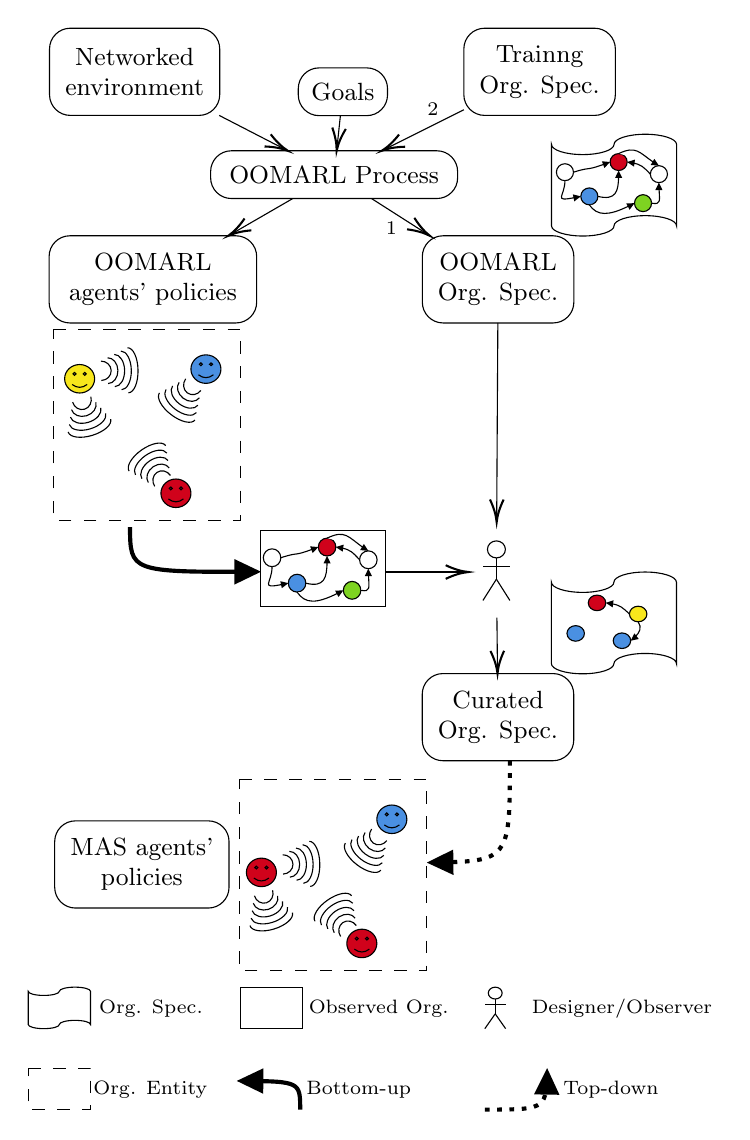
\begin{tikzpicture}[x=0.75pt,y=0.75pt,yscale=-1,xscale=1]
%uncomment if require: \path (0,567); %set diagram left start at 0, and has height of 567

%Flowchart: Punched Tape [id:dp09352793636343182] 
\draw  [fill={rgb, 255:red, 255; green, 255; blue, 255 }  ,fill opacity=1 ] (260,284.9) .. controls (260,287.61) and (266.74,289.81) .. (275.06,289.81) .. controls (283.38,289.81) and (290.12,287.61) .. (290.12,284.9) .. controls (290.12,282.2) and (296.87,280) .. (305.18,280) .. controls (313.5,280) and (320.25,282.2) .. (320.25,284.9) -- (320.25,324.13) .. controls (320.25,321.42) and (313.5,319.23) .. (305.18,319.23) .. controls (296.87,319.23) and (290.12,321.42) .. (290.12,324.13) .. controls (290.12,326.84) and (283.38,329.03) .. (275.06,329.03) .. controls (266.74,329.03) and (260,326.84) .. (260,324.13) -- cycle ;
%Shape: Ellipse [id:dp8537944349912123] 
\draw  [fill={rgb, 255:red, 208; green, 2; blue, 27 }  ,fill opacity=1 ] (277.77,294.86) .. controls (277.77,292.79) and (279.66,291.11) .. (281.98,291.11) .. controls (284.3,291.11) and (286.19,292.79) .. (286.19,294.86) .. controls (286.19,296.94) and (284.3,298.62) .. (281.98,298.62) .. controls (279.66,298.62) and (277.77,296.94) .. (277.77,294.86) -- cycle ;
%Shape: Ellipse [id:dp6897748103188357] 
\draw  [fill={rgb, 255:red, 248; green, 231; blue, 28 }  ,fill opacity=1 ] (297.6,300.23) .. controls (297.6,298.15) and (299.49,296.47) .. (301.81,296.47) .. controls (304.13,296.47) and (306.02,298.15) .. (306.02,300.23) .. controls (306.02,302.3) and (304.13,303.98) .. (301.81,303.98) .. controls (299.49,303.98) and (297.6,302.3) .. (297.6,300.23) -- cycle ;
%Shape: Ellipse [id:dp4802320082509959] 
\draw  [fill={rgb, 255:red, 74; green, 144; blue, 226 }  ,fill opacity=1 ] (289.79,313.09) .. controls (289.79,311.02) and (291.67,309.34) .. (294,309.34) .. controls (296.32,309.34) and (298.2,311.02) .. (298.2,313.09) .. controls (298.2,315.17) and (296.32,316.85) .. (294,316.85) .. controls (291.67,316.85) and (289.79,315.17) .. (289.79,313.09) -- cycle ;
%Curve Lines [id:da7546101861138359] 
\draw [fill={rgb, 255:red, 255; green, 255; blue, 255 }  ,fill opacity=1 ]   (297.6,300.23) .. controls (294.11,296.93) and (293.1,296) .. (289.08,295.29) ;
\draw [shift={(286.19,294.86)}, rotate = 7.39] [fill={rgb, 255:red, 0; green, 0; blue, 0 }  ][line width=0.08]  [draw opacity=0] (3.57,-1.72) -- (0,0) -- (3.57,1.72) -- cycle    ;
%Shape: Ellipse [id:dp693668966316707] 
\draw  [fill={rgb, 255:red, 74; green, 144; blue, 226 }  ,fill opacity=1 ] (267.5,309.58) .. controls (267.5,307.51) and (269.38,305.83) .. (271.71,305.83) .. controls (274.03,305.83) and (275.91,307.51) .. (275.91,309.58) .. controls (275.91,311.65) and (274.03,313.33) .. (271.71,313.33) .. controls (269.38,313.33) and (267.5,311.65) .. (267.5,309.58) -- cycle ;
%Curve Lines [id:da5612242217579502] 
\draw [fill={rgb, 255:red, 255; green, 255; blue, 255 }  ,fill opacity=1 ]   (301.81,303.98) .. controls (303.69,306.69) and (302.57,309.05) .. (300.45,311.16) ;
\draw [shift={(298.2,313.09)}, rotate = 322.38] [fill={rgb, 255:red, 0; green, 0; blue, 0 }  ][line width=0.08]  [draw opacity=0] (3.57,-1.72) -- (0,0) -- (3.57,1.72) -- cycle    ;

%Shape: Rectangle [id:dp7949048767988509] 
\draw  [dash pattern={on 4.5pt off 4.5pt}] (20.05,163.11) -- (110.42,163.11) -- (110.42,255.04) -- (20.05,255.04) -- cycle ;
%Shape: Smiley Face [id:dp8425156316307105] 
\draw  [fill={rgb, 255:red, 248; green, 231; blue, 28 }  ,fill opacity=1 ] (25.48,186.89) .. controls (25.48,183.1) and (28.71,180.03) .. (32.71,180.03) .. controls (36.7,180.03) and (39.94,183.1) .. (39.94,186.89) .. controls (39.94,190.68) and (36.7,193.75) .. (32.71,193.75) .. controls (28.71,193.75) and (25.48,190.68) .. (25.48,186.89) -- cycle ; \draw  [fill={rgb, 255:red, 248; green, 231; blue, 28 }  ,fill opacity=1 ] (29.53,184.56) .. controls (29.53,184.18) and (29.85,183.87) .. (30.25,183.87) .. controls (30.65,183.87) and (30.97,184.18) .. (30.97,184.56) .. controls (30.97,184.94) and (30.65,185.24) .. (30.25,185.24) .. controls (29.85,185.24) and (29.53,184.94) .. (29.53,184.56) -- cycle ; \draw  [fill={rgb, 255:red, 248; green, 231; blue, 28 }  ,fill opacity=1 ] (34.44,184.56) .. controls (34.44,184.18) and (34.77,183.87) .. (35.16,183.87) .. controls (35.56,183.87) and (35.89,184.18) .. (35.89,184.56) .. controls (35.89,184.94) and (35.56,185.24) .. (35.16,185.24) .. controls (34.77,185.24) and (34.44,184.94) .. (34.44,184.56) -- cycle ; \draw   (29.09,189.64) .. controls (31.5,191.47) and (33.91,191.47) .. (36.32,189.64) ;
%Shape: Arc [id:dp7103754459108031] 
\draw  [draw opacity=0] (47.66,206.32) .. controls (47.66,206.32) and (47.66,206.32) .. (47.66,206.32) .. controls (48.43,208.93) and (44.47,212.43) .. (38.81,214.15) .. controls (33.16,215.87) and (27.96,215.15) .. (27.19,212.54) -- (37.43,209.43) -- cycle ; \draw   (47.66,206.32) .. controls (47.66,206.32) and (47.66,206.32) .. (47.66,206.32) .. controls (48.43,208.93) and (44.47,212.43) .. (38.81,214.15) .. controls (33.16,215.87) and (27.96,215.15) .. (27.19,212.54) ;  
%Shape: Arc [id:dp9993647702991559] 
\draw  [draw opacity=0] (45.27,203.61) .. controls (46.04,206.22) and (42.73,209.53) .. (37.89,211) .. controls (33.04,212.48) and (28.49,211.55) .. (27.73,208.94) -- (36.5,206.28) -- cycle ; \draw   (45.27,203.61) .. controls (46.04,206.22) and (42.73,209.53) .. (37.89,211) .. controls (33.04,212.48) and (28.49,211.55) .. (27.73,208.94) ;  
%Shape: Arc [id:dp33021260729129986] 
\draw  [draw opacity=0] (42.88,200.9) .. controls (42.88,200.9) and (42.88,200.9) .. (42.88,200.9) .. controls (43.65,203.51) and (41,206.62) .. (36.96,207.85) .. controls (32.92,209.08) and (29.03,207.96) .. (28.26,205.35) -- (35.57,203.12) -- cycle ; \draw   (42.88,200.9) .. controls (42.88,200.9) and (42.88,200.9) .. (42.88,200.9) .. controls (43.65,203.51) and (41,206.62) .. (36.96,207.85) .. controls (32.92,209.08) and (29.03,207.96) .. (28.26,205.35) ;  
%Shape: Arc [id:dp7515950702187679] 
\draw  [draw opacity=0] (40.5,198.2) .. controls (40.5,198.2) and (40.5,198.2) .. (40.5,198.2) .. controls (40.5,198.2) and (40.5,198.2) .. (40.5,198.2) .. controls (41.26,200.81) and (39.27,203.72) .. (36.04,204.7) .. controls (32.81,205.68) and (29.57,204.36) .. (28.8,201.75) .. controls (28.8,201.75) and (28.8,201.75) .. (28.8,201.75) -- (34.65,199.97) -- cycle ; \draw   (40.5,198.2) .. controls (40.5,198.2) and (40.5,198.2) .. (40.5,198.2) .. controls (40.5,198.2) and (40.5,198.2) .. (40.5,198.2) .. controls (41.26,200.81) and (39.27,203.72) .. (36.04,204.7) .. controls (32.81,205.68) and (29.57,204.36) .. (28.8,201.75) .. controls (28.8,201.75) and (28.8,201.75) .. (28.8,201.75) ;  
%Shape: Arc [id:dp17995425823285305] 
\draw  [draw opacity=0] (38.11,195.49) .. controls (38.11,195.49) and (38.11,195.49) .. (38.11,195.49) .. controls (38.11,195.49) and (38.11,195.49) .. (38.11,195.49) .. controls (38.88,198.1) and (37.53,200.81) .. (35.11,201.55) .. controls (32.69,202.29) and (30.1,200.77) .. (29.34,198.16) -- (33.72,196.82) -- cycle ; \draw   (38.11,195.49) .. controls (38.11,195.49) and (38.11,195.49) .. (38.11,195.49) .. controls (38.11,195.49) and (38.11,195.49) .. (38.11,195.49) .. controls (38.88,198.1) and (37.53,200.81) .. (35.11,201.55) .. controls (32.69,202.29) and (30.1,200.77) .. (29.34,198.16) ;  

%Shape: Arc [id:dp8934563741256025] 
\draw  [draw opacity=0] (55.78,171.93) .. controls (58.46,171.87) and (60.73,176.69) .. (60.84,182.69) .. controls (60.96,188.7) and (58.88,193.6) .. (56.21,193.66) -- (55.99,182.79) -- cycle ; \draw   (55.78,171.93) .. controls (58.46,171.87) and (60.73,176.69) .. (60.84,182.69) .. controls (60.96,188.7) and (58.88,193.6) .. (56.21,193.66) ;  
%Shape: Arc [id:dp5963815446588989] 
\draw  [draw opacity=0] (52.58,173.54) .. controls (55.26,173.49) and (57.51,177.62) .. (57.61,182.76) .. controls (57.71,187.9) and (55.62,192.12) .. (52.94,192.17) -- (52.76,182.86) -- cycle ; \draw   (52.58,173.54) .. controls (55.26,173.49) and (57.51,177.62) .. (57.61,182.76) .. controls (57.71,187.9) and (55.62,192.12) .. (52.94,192.17) ;  
%Shape: Arc [id:dp3378668028957823] 
\draw  [draw opacity=0] (49.38,175.16) .. controls (49.38,175.16) and (49.38,175.16) .. (49.38,175.16) .. controls (49.38,175.16) and (49.38,175.16) .. (49.38,175.16) .. controls (52.06,175.11) and (54.3,178.54) .. (54.38,182.82) .. controls (54.46,187.11) and (52.36,190.63) .. (49.68,190.68) -- (49.53,182.92) -- cycle ; \draw   (49.38,175.16) .. controls (49.38,175.16) and (49.38,175.16) .. (49.38,175.16) .. controls (49.38,175.16) and (49.38,175.16) .. (49.38,175.16) .. controls (52.06,175.11) and (54.3,178.54) .. (54.38,182.82) .. controls (54.46,187.11) and (52.36,190.63) .. (49.68,190.68) ;  
%Shape: Arc [id:dp7870035207223711] 
\draw  [draw opacity=0] (46.18,176.78) .. controls (48.86,176.72) and (51.08,179.46) .. (51.15,182.89) .. controls (51.21,186.32) and (49.1,189.14) .. (46.42,189.2) -- (46.3,182.99) -- cycle ; \draw   (46.18,176.78) .. controls (48.86,176.72) and (51.08,179.46) .. (51.15,182.89) .. controls (51.21,186.32) and (49.1,189.14) .. (46.42,189.2) ;  
%Shape: Arc [id:dp7731275981870975] 
\draw  [draw opacity=0] (42.98,178.39) .. controls (42.98,178.39) and (42.98,178.39) .. (42.98,178.39) .. controls (45.65,178.34) and (47.86,180.38) .. (47.91,182.95) .. controls (47.96,185.53) and (45.83,187.65) .. (43.16,187.71) -- (43.07,183.05) -- cycle ; \draw   (42.98,178.39) .. controls (42.98,178.39) and (42.98,178.39) .. (42.98,178.39) .. controls (45.65,178.34) and (47.86,180.38) .. (47.91,182.95) .. controls (47.96,185.53) and (45.83,187.65) .. (43.16,187.71) ;  

%Shape: Smiley Face [id:dp9460068866596214] 
\draw  [fill={rgb, 255:red, 208; green, 2; blue, 27 }  ,fill opacity=1 ] (71.87,242.05) .. controls (71.87,238.26) and (75.1,235.19) .. (79.1,235.19) .. controls (83.09,235.19) and (86.33,238.26) .. (86.33,242.05) .. controls (86.33,245.84) and (83.09,248.92) .. (79.1,248.92) .. controls (75.1,248.92) and (71.87,245.84) .. (71.87,242.05) -- cycle ; \draw  [fill={rgb, 255:red, 208; green, 2; blue, 27 }  ,fill opacity=1 ] (75.91,239.72) .. controls (75.91,239.34) and (76.24,239.03) .. (76.64,239.03) .. controls (77.04,239.03) and (77.36,239.34) .. (77.36,239.72) .. controls (77.36,240.1) and (77.04,240.4) .. (76.64,240.4) .. controls (76.24,240.4) and (75.91,240.1) .. (75.91,239.72) -- cycle ; \draw  [fill={rgb, 255:red, 208; green, 2; blue, 27 }  ,fill opacity=1 ] (80.83,239.72) .. controls (80.83,239.34) and (81.15,239.03) .. (81.55,239.03) .. controls (81.95,239.03) and (82.28,239.34) .. (82.28,239.72) .. controls (82.28,240.1) and (81.95,240.4) .. (81.55,240.4) .. controls (81.15,240.4) and (80.83,240.1) .. (80.83,239.72) -- cycle ; \draw   (75.48,244.8) .. controls (77.89,246.63) and (80.3,246.63) .. (82.71,244.8) ;
%Shape: Arc [id:dp2662505393390908] 
\draw  [draw opacity=0] (56.53,231.38) .. controls (56.53,231.38) and (56.53,231.38) .. (56.53,231.38) .. controls (56.53,231.38) and (56.53,231.38) .. (56.53,231.38) .. controls (55.02,229.13) and (57.74,224.56) .. (62.6,221.17) .. controls (67.47,217.77) and (72.64,216.84) .. (74.15,219.09) -- (65.34,225.24) -- cycle ; \draw   (56.53,231.38) .. controls (56.53,231.38) and (56.53,231.38) .. (56.53,231.38) .. controls (56.53,231.38) and (56.53,231.38) .. (56.53,231.38) .. controls (55.02,229.13) and (57.74,224.56) .. (62.6,221.17) .. controls (67.47,217.77) and (72.64,216.84) .. (74.15,219.09) ;  
%Shape: Arc [id:dp5533657200850002] 
\draw  [draw opacity=0] (59.62,233.22) .. controls (59.62,233.22) and (59.62,233.22) .. (59.62,233.22) .. controls (58.11,230.97) and (60.26,226.79) .. (64.43,223.88) .. controls (68.6,220.97) and (73.21,220.43) .. (74.72,222.68) -- (67.17,227.95) -- cycle ; \draw   (59.62,233.22) .. controls (59.62,233.22) and (59.62,233.22) .. (59.62,233.22) .. controls (58.11,230.97) and (60.26,226.79) .. (64.43,223.88) .. controls (68.6,220.97) and (73.21,220.43) .. (74.72,222.68) ;  
%Shape: Arc [id:dp130720604660594] 
\draw  [draw opacity=0] (62.71,235.05) .. controls (61.19,232.8) and (62.78,229.02) .. (66.26,226.59) .. controls (69.73,224.17) and (73.78,224.02) .. (75.29,226.27) -- (69,230.66) -- cycle ; \draw   (62.71,235.05) .. controls (61.19,232.8) and (62.78,229.02) .. (66.26,226.59) .. controls (69.73,224.17) and (73.78,224.02) .. (75.29,226.27) ;  
%Shape: Arc [id:dp7777326608896638] 
\draw  [draw opacity=0] (65.79,236.88) .. controls (65.79,236.88) and (65.79,236.88) .. (65.79,236.88) .. controls (64.28,234.64) and (65.31,231.24) .. (68.09,229.3) .. controls (70.87,227.36) and (74.35,227.61) .. (75.86,229.86) -- (70.83,233.37) -- cycle ; \draw   (65.79,236.88) .. controls (65.79,236.88) and (65.79,236.88) .. (65.79,236.88) .. controls (64.28,234.64) and (65.31,231.24) .. (68.09,229.3) .. controls (70.87,227.36) and (74.35,227.61) .. (75.86,229.86) ;  
%Shape: Arc [id:dp4348101062357661] 
\draw  [draw opacity=0] (68.88,238.72) .. controls (67.37,236.47) and (67.83,233.47) .. (69.92,232.02) .. controls (72,230.56) and (74.92,231.2) .. (76.43,233.45) -- (72.66,236.08) -- cycle ; \draw   (68.88,238.72) .. controls (67.37,236.47) and (67.83,233.47) .. (69.92,232.02) .. controls (72,230.56) and (74.92,231.2) .. (76.43,233.45) ;  

%Shape: Smiley Face [id:dp40321958667865143] 
\draw  [fill={rgb, 255:red, 74; green, 144; blue, 226 }  ,fill opacity=1 ] (86.33,182.23) .. controls (86.33,178.44) and (89.56,175.37) .. (93.55,175.37) .. controls (97.55,175.37) and (100.78,178.44) .. (100.78,182.23) .. controls (100.78,186.02) and (97.55,189.1) .. (93.55,189.1) .. controls (89.56,189.1) and (86.33,186.02) .. (86.33,182.23) -- cycle ; \draw  [fill={rgb, 255:red, 74; green, 144; blue, 226 }  ,fill opacity=1 ] (90.37,179.9) .. controls (90.37,179.52) and (90.7,179.21) .. (91.1,179.21) .. controls (91.5,179.21) and (91.82,179.52) .. (91.82,179.9) .. controls (91.82,180.28) and (91.5,180.58) .. (91.1,180.58) .. controls (90.7,180.58) and (90.37,180.28) .. (90.37,179.9) -- cycle ; \draw  [fill={rgb, 255:red, 74; green, 144; blue, 226 }  ,fill opacity=1 ] (95.29,179.9) .. controls (95.29,179.52) and (95.61,179.21) .. (96.01,179.21) .. controls (96.41,179.21) and (96.74,179.52) .. (96.74,179.9) .. controls (96.74,180.28) and (96.41,180.58) .. (96.01,180.58) .. controls (95.61,180.58) and (95.29,180.28) .. (95.29,179.9) -- cycle ; \draw   (89.94,184.98) .. controls (92.35,186.81) and (94.76,186.81) .. (97.17,184.98) ;
%Shape: Arc [id:dp6344973920370733] 
\draw  [draw opacity=0] (88.26,206.75) .. controls (88.26,206.75) and (88.26,206.75) .. (88.26,206.75) .. controls (86.65,208.93) and (81.52,207.78) .. (76.8,204.18) .. controls (72.08,200.58) and (69.55,195.9) .. (71.16,193.72) -- (79.71,200.23) -- cycle ; \draw   (88.26,206.75) .. controls (88.26,206.75) and (88.26,206.75) .. (88.26,206.75) .. controls (86.65,208.93) and (81.52,207.78) .. (76.8,204.18) .. controls (72.08,200.58) and (69.55,195.9) .. (71.16,193.72) ;  
%Shape: Arc [id:dp2502725185770005] 
\draw  [draw opacity=0] (88.97,203.19) .. controls (88.97,203.19) and (88.97,203.19) .. (88.97,203.19) .. controls (88.97,203.19) and (88.97,203.19) .. (88.97,203.19) .. controls (87.37,205.37) and (82.78,204.63) .. (78.74,201.55) .. controls (74.69,198.46) and (72.71,194.2) .. (74.32,192.02) -- (81.65,197.6) -- cycle ; \draw   (88.97,203.19) .. controls (88.97,203.19) and (88.97,203.19) .. (88.97,203.19) .. controls (88.97,203.19) and (88.97,203.19) .. (88.97,203.19) .. controls (87.37,205.37) and (82.78,204.63) .. (78.74,201.55) .. controls (74.69,198.46) and (72.71,194.2) .. (74.32,192.02) ;  
%Shape: Arc [id:dp23421846029392612] 
\draw  [draw opacity=0] (89.69,199.63) .. controls (89.69,199.63) and (89.69,199.63) .. (89.69,199.63) .. controls (89.69,199.63) and (89.69,199.63) .. (89.69,199.63) .. controls (88.08,201.81) and (84.05,201.49) .. (80.68,198.92) .. controls (77.3,196.35) and (75.87,192.5) .. (77.48,190.32) -- (83.58,194.97) -- cycle ; \draw   (89.69,199.63) .. controls (89.69,199.63) and (89.69,199.63) .. (89.69,199.63) .. controls (89.69,199.63) and (89.69,199.63) .. (89.69,199.63) .. controls (88.08,201.81) and (84.05,201.49) .. (80.68,198.92) .. controls (77.3,196.35) and (75.87,192.5) .. (77.48,190.32) ;  
%Shape: Arc [id:dp02946644855410807] 
\draw  [draw opacity=0] (90.41,196.06) .. controls (88.8,198.24) and (85.31,198.34) .. (82.62,196.29) .. controls (79.92,194.23) and (79.03,190.8) .. (80.64,188.62) -- (85.52,192.34) -- cycle ; \draw   (90.41,196.06) .. controls (88.8,198.24) and (85.31,198.34) .. (82.62,196.29) .. controls (79.92,194.23) and (79.03,190.8) .. (80.64,188.62) ;  
%Shape: Arc [id:dp07919277634076938] 
\draw  [draw opacity=0] (91.13,192.5) .. controls (91.13,192.5) and (91.13,192.5) .. (91.13,192.5) .. controls (89.52,194.68) and (86.58,195.2) .. (84.55,193.66) .. controls (82.53,192.11) and (82.19,189.1) .. (83.8,186.92) -- (87.46,189.71) -- cycle ; \draw   (91.13,192.5) .. controls (91.13,192.5) and (91.13,192.5) .. (91.13,192.5) .. controls (89.52,194.68) and (86.58,195.2) .. (84.55,193.66) .. controls (82.53,192.11) and (82.19,189.1) .. (83.8,186.92) ;  

%Shape: Ellipse [id:dp5665300419613197] 
\draw   (229.18,269.1) .. controls (229.18,266.84) and (231.12,265) .. (233.51,265) .. controls (235.9,265) and (237.84,266.84) .. (237.84,269.1) .. controls (237.84,271.36) and (235.9,273.2) .. (233.51,273.2) .. controls (231.12,273.2) and (229.18,271.36) .. (229.18,269.1) -- cycle ;
%Straight Lines [id:da868287133321088] 
\draw    (233.51,273.2) -- (233.51,283.45) ;
%Straight Lines [id:da7338999456859931] 
\draw    (233.51,283.45) -- (227.02,293.7) ;
%Straight Lines [id:da7618645013452761] 
\draw    (233.51,283.45) -- (240,293.7) ;
%Straight Lines [id:da7029210082761028] 
\draw    (240,277.3) -- (227.02,277.3) ;

%Shape: Rectangle [id:dp36259598060414655] 
\draw  [fill={rgb, 255:red, 255; green, 255; blue, 255 }  ,fill opacity=1 ] (120,260) -- (180.25,260) -- (180.25,296.77) -- (120,296.77) -- cycle ;
%Shape: Ellipse [id:dp34598635042601256] 
\draw  [fill={rgb, 255:red, 255; green, 255; blue, 255 }  ,fill opacity=1 ] (121.2,273.12) .. controls (121.2,270.75) and (123.09,268.83) .. (125.42,268.83) .. controls (127.75,268.83) and (129.64,270.75) .. (129.64,273.12) .. controls (129.64,275.49) and (127.75,277.41) .. (125.42,277.41) .. controls (123.09,277.41) and (121.2,275.49) .. (121.2,273.12) -- cycle ;
%Shape: Ellipse [id:dp0011247415244253212] 
\draw  [fill={rgb, 255:red, 74; green, 144; blue, 226 }  ,fill opacity=1 ] (133.25,285.37) .. controls (133.25,283) and (135.14,281.08) .. (137.47,281.08) .. controls (139.8,281.08) and (141.69,283) .. (141.69,285.37) .. controls (141.69,287.74) and (139.8,289.66) .. (137.47,289.66) .. controls (135.14,289.66) and (133.25,287.74) .. (133.25,285.37) -- cycle ;
%Shape: Ellipse [id:dp8822927144483022] 
\draw  [fill={rgb, 255:red, 208; green, 2; blue, 27 }  ,fill opacity=1 ] (147.71,267.97) .. controls (147.71,265.6) and (149.6,263.68) .. (151.93,263.68) .. controls (154.26,263.68) and (156.15,265.6) .. (156.15,267.97) .. controls (156.15,270.34) and (154.26,272.26) .. (151.93,272.26) .. controls (149.6,272.26) and (147.71,270.34) .. (147.71,267.97) -- cycle ;
%Shape: Ellipse [id:dp7611446545020739] 
\draw  [fill={rgb, 255:red, 255; green, 255; blue, 255 }  ,fill opacity=1 ] (167.59,274.1) .. controls (167.59,271.73) and (169.48,269.81) .. (171.81,269.81) .. controls (174.14,269.81) and (176.03,271.73) .. (176.03,274.1) .. controls (176.03,276.47) and (174.14,278.39) .. (171.81,278.39) .. controls (169.48,278.39) and (167.59,276.47) .. (167.59,274.1) -- cycle ;
%Shape: Ellipse [id:dp1592826898001829] 
\draw  [fill={rgb, 255:red, 126; green, 211; blue, 33 }  ,fill opacity=1 ] (159.76,288.81) .. controls (159.76,286.44) and (161.65,284.52) .. (163.98,284.52) .. controls (166.31,284.52) and (168.2,286.44) .. (168.2,288.81) .. controls (168.2,291.18) and (166.31,293.1) .. (163.98,293.1) .. controls (161.65,293.1) and (159.76,291.18) .. (159.76,288.81) -- cycle ;
%Curve Lines [id:da27399536046205264] 
\draw [fill={rgb, 255:red, 255; green, 255; blue, 255 }  ,fill opacity=1 ]   (129.64,273.12) .. controls (139.11,270.05) and (134.67,272.76) .. (144.92,269.01) ;
\draw [shift={(147.71,267.97)}, rotate = 159.17] [fill={rgb, 255:red, 0; green, 0; blue, 0 }  ][line width=0.08]  [draw opacity=0] (3.57,-1.72) -- (0,0) -- (3.57,1.72) -- cycle    ;
%Curve Lines [id:da16623917428090795] 
\draw [fill={rgb, 255:red, 255; green, 255; blue, 255 }  ,fill opacity=1 ]   (141.69,285.37) .. controls (150.75,287.65) and (151.79,282.63) .. (151.91,275.25) ;
\draw [shift={(151.93,272.26)}, rotate = 90] [fill={rgb, 255:red, 0; green, 0; blue, 0 }  ][line width=0.08]  [draw opacity=0] (3.57,-1.72) -- (0,0) -- (3.57,1.72) -- cycle    ;
%Curve Lines [id:da46234775845087284] 
\draw [fill={rgb, 255:red, 255; green, 255; blue, 255 }  ,fill opacity=1 ]   (167.59,274.1) .. controls (164.09,270.33) and (163.08,269.27) .. (159.05,268.46) ;
\draw [shift={(156.15,267.97)}, rotate = 8.42] [fill={rgb, 255:red, 0; green, 0; blue, 0 }  ][line width=0.08]  [draw opacity=0] (3.57,-1.72) -- (0,0) -- (3.57,1.72) -- cycle    ;
%Curve Lines [id:da3119386523209393] 
\draw [fill={rgb, 255:red, 255; green, 255; blue, 255 }  ,fill opacity=1 ]   (168.2,288.81) .. controls (172.97,289.67) and (172.14,287.87) .. (171.87,281.33) ;
\draw [shift={(171.81,278.39)}, rotate = 90] [fill={rgb, 255:red, 0; green, 0; blue, 0 }  ][line width=0.08]  [draw opacity=0] (3.57,-1.72) -- (0,0) -- (3.57,1.72) -- cycle    ;
%Curve Lines [id:da8983756138417751] 
\draw [fill={rgb, 255:red, 255; green, 255; blue, 255 }  ,fill opacity=1 ]   (125.42,277.41) .. controls (125.42,285.5) and (119.17,288.19) .. (130.41,285.96) ;
\draw [shift={(133.25,285.37)}, rotate = 168.05] [fill={rgb, 255:red, 0; green, 0; blue, 0 }  ][line width=0.08]  [draw opacity=0] (3.57,-1.72) -- (0,0) -- (3.57,1.72) -- cycle    ;
%Curve Lines [id:da8579733900345894] 
\draw [fill={rgb, 255:red, 255; green, 255; blue, 255 }  ,fill opacity=1 ]   (137.47,289.66) .. controls (141.37,295.45) and (146.82,295.36) .. (157.15,290.17) ;
\draw [shift={(159.76,288.81)}, rotate = 151.67] [fill={rgb, 255:red, 0; green, 0; blue, 0 }  ][line width=0.08]  [draw opacity=0] (3.57,-1.72) -- (0,0) -- (3.57,1.72) -- cycle    ;
%Curve Lines [id:da598997074659714] 
\draw [fill={rgb, 255:red, 255; green, 255; blue, 255 }  ,fill opacity=1 ]   (151.93,263.68) .. controls (160.7,259.44) and (161.99,263.12) .. (169.42,268.25) ;
\draw [shift={(171.81,269.81)}, rotate = 211.4] [fill={rgb, 255:red, 0; green, 0; blue, 0 }  ][line width=0.08]  [draw opacity=0] (3.57,-1.72) -- (0,0) -- (3.57,1.72) -- cycle    ;

%Shape: Boxed Bezier Curve [id:dp04329100663395624] 
\draw [line width=1.5]    (56.97,258.4) .. controls (57.12,279.64) and (57.12,280.06) .. (116.36,279.88) ;
\draw [shift={(120.07,279.86)}, rotate = 179.81] [fill={rgb, 255:red, 0; green, 0; blue, 0 }  ][line width=0.08]  [draw opacity=0] (12.77,-6.13) -- (0,0) -- (12.77,6.13) -- cycle    ;
%Shape: Boxed Bezier Curve [id:dp3249540323733473] 
\draw [line width=1.5]  [dash pattern={on 1.69pt off 2.76pt}]  (240,371) .. controls (240,377.31) and (240,382.8) .. (239.91,387.58) .. controls (239.34,418.4) and (235.11,419.53) .. (203.54,419.96) ;
\draw [shift={(200,420)}, rotate = 359.3] [fill={rgb, 255:red, 0; green, 0; blue, 0 }  ][line width=0.08]  [draw opacity=0] (12.77,-6.13) -- (0,0) -- (12.77,6.13) -- cycle    ;
%Shape: Rectangle [id:dp3591393250200341] 
\draw  [dash pattern={on 4.5pt off 4.5pt}] (109.63,380) -- (200,380) -- (200,471.94) -- (109.63,471.94) -- cycle ;
%Shape: Smiley Face [id:dp3801591887945033] 
\draw  [fill={rgb, 255:red, 208; green, 2; blue, 27 }  ,fill opacity=1 ] (113.05,424.72) .. controls (113.05,420.92) and (116.29,417.85) .. (120.28,417.85) .. controls (124.28,417.85) and (127.51,420.92) .. (127.51,424.72) .. controls (127.51,428.51) and (124.28,431.58) .. (120.28,431.58) .. controls (116.29,431.58) and (113.05,428.51) .. (113.05,424.72) -- cycle ; \draw  [fill={rgb, 255:red, 208; green, 2; blue, 27 }  ,fill opacity=1 ] (117.1,422.38) .. controls (117.1,422) and (117.43,421.7) .. (117.82,421.7) .. controls (118.22,421.7) and (118.55,422) .. (118.55,422.38) .. controls (118.55,422.76) and (118.22,423.07) .. (117.82,423.07) .. controls (117.43,423.07) and (117.1,422.76) .. (117.1,422.38) -- cycle ; \draw  [fill={rgb, 255:red, 208; green, 2; blue, 27 }  ,fill opacity=1 ] (122.02,422.38) .. controls (122.02,422) and (122.34,421.7) .. (122.74,421.7) .. controls (123.14,421.7) and (123.46,422) .. (123.46,422.38) .. controls (123.46,422.76) and (123.14,423.07) .. (122.74,423.07) .. controls (122.34,423.07) and (122.02,422.76) .. (122.02,422.38) -- cycle ; \draw   (116.67,427.46) .. controls (119.08,429.29) and (121.49,429.29) .. (123.9,427.46) ;
%Shape: Arc [id:dp40222913228483237] 
\draw  [draw opacity=0] (135.24,444.14) .. controls (135.24,444.14) and (135.24,444.14) .. (135.24,444.14) .. controls (136,446.75) and (132.04,450.26) .. (126.39,451.98) .. controls (120.74,453.7) and (115.53,452.97) .. (114.77,450.36) -- (125,447.25) -- cycle ; \draw   (135.24,444.14) .. controls (135.24,444.14) and (135.24,444.14) .. (135.24,444.14) .. controls (136,446.75) and (132.04,450.26) .. (126.39,451.98) .. controls (120.74,453.7) and (115.53,452.97) .. (114.77,450.36) ;  
%Shape: Arc [id:dp6185790641450695] 
\draw  [draw opacity=0] (132.85,441.43) .. controls (133.62,444.05) and (130.31,447.36) .. (125.46,448.83) .. controls (120.62,450.3) and (116.07,449.38) .. (115.3,446.77) -- (124.08,444.1) -- cycle ; \draw   (132.85,441.43) .. controls (133.62,444.05) and (130.31,447.36) .. (125.46,448.83) .. controls (120.62,450.3) and (116.07,449.38) .. (115.3,446.77) ;  
%Shape: Arc [id:dp6749114191148724] 
\draw  [draw opacity=0] (130.46,438.73) .. controls (130.46,438.73) and (130.46,438.73) .. (130.46,438.73) .. controls (131.23,441.34) and (128.58,444.45) .. (124.54,445.68) .. controls (120.5,446.9) and (116.61,445.78) .. (115.84,443.17) -- (123.15,440.95) -- cycle ; \draw   (130.46,438.73) .. controls (130.46,438.73) and (130.46,438.73) .. (130.46,438.73) .. controls (131.23,441.34) and (128.58,444.45) .. (124.54,445.68) .. controls (120.5,446.9) and (116.61,445.78) .. (115.84,443.17) ;  
%Shape: Arc [id:dp056403546095020296] 
\draw  [draw opacity=0] (128.07,436.02) .. controls (128.07,436.02) and (128.07,436.02) .. (128.07,436.02) .. controls (128.07,436.02) and (128.07,436.02) .. (128.07,436.02) .. controls (128.84,438.63) and (126.84,441.54) .. (123.61,442.53) .. controls (120.38,443.51) and (117.14,442.19) .. (116.38,439.58) -- (122.22,437.8) -- cycle ; \draw   (128.07,436.02) .. controls (128.07,436.02) and (128.07,436.02) .. (128.07,436.02) .. controls (128.07,436.02) and (128.07,436.02) .. (128.07,436.02) .. controls (128.84,438.63) and (126.84,441.54) .. (123.61,442.53) .. controls (120.38,443.51) and (117.14,442.19) .. (116.38,439.58) ;  
%Shape: Arc [id:dp048963270262922354] 
\draw  [draw opacity=0] (125.69,433.32) .. controls (125.69,433.32) and (125.69,433.32) .. (125.69,433.32) .. controls (126.45,435.93) and (125.11,438.64) .. (122.69,439.38) .. controls (120.27,440.11) and (117.68,438.59) .. (116.91,435.98) -- (121.3,434.65) -- cycle ; \draw   (125.69,433.32) .. controls (125.69,433.32) and (125.69,433.32) .. (125.69,433.32) .. controls (126.45,435.93) and (125.11,438.64) .. (122.69,439.38) .. controls (120.27,440.11) and (117.68,438.59) .. (116.91,435.98) ;  

%Shape: Arc [id:dp11791815378481285] 
\draw  [draw opacity=0] (143.36,409.75) .. controls (143.36,409.75) and (143.36,409.75) .. (143.36,409.75) .. controls (146.04,409.7) and (148.3,414.52) .. (148.42,420.52) .. controls (148.54,426.52) and (146.46,431.43) .. (143.78,431.48) -- (143.57,420.62) -- cycle ; \draw   (143.36,409.75) .. controls (143.36,409.75) and (143.36,409.75) .. (143.36,409.75) .. controls (146.04,409.7) and (148.3,414.52) .. (148.42,420.52) .. controls (148.54,426.52) and (146.46,431.43) .. (143.78,431.48) ;  
%Shape: Arc [id:dp6186444432706435] 
\draw  [draw opacity=0] (140.16,411.37) .. controls (142.84,411.32) and (145.09,415.44) .. (145.19,420.59) .. controls (145.29,425.73) and (143.2,429.94) .. (140.52,430) -- (140.34,420.68) -- cycle ; \draw   (140.16,411.37) .. controls (142.84,411.32) and (145.09,415.44) .. (145.19,420.59) .. controls (145.29,425.73) and (143.2,429.94) .. (140.52,430) ;  
%Shape: Arc [id:dp3524256769019909] 
\draw  [draw opacity=0] (136.96,412.99) .. controls (136.96,412.99) and (136.96,412.99) .. (136.96,412.99) .. controls (139.63,412.93) and (141.87,416.36) .. (141.96,420.65) .. controls (142.04,424.94) and (139.94,428.45) .. (137.26,428.51) .. controls (137.26,428.51) and (137.26,428.51) .. (137.26,428.51) -- (137.11,420.75) -- cycle ; \draw   (136.96,412.99) .. controls (136.96,412.99) and (136.96,412.99) .. (136.96,412.99) .. controls (139.63,412.93) and (141.87,416.36) .. (141.96,420.65) .. controls (142.04,424.94) and (139.94,428.45) .. (137.26,428.51) .. controls (137.26,428.51) and (137.26,428.51) .. (137.26,428.51) ;  
%Shape: Arc [id:dp9364872182962407] 
\draw  [draw opacity=0] (133.76,414.6) .. controls (136.43,414.55) and (138.66,417.29) .. (138.72,420.72) .. controls (138.79,424.14) and (136.67,426.97) .. (134,427.02) -- (133.88,420.81) -- cycle ; \draw   (133.76,414.6) .. controls (136.43,414.55) and (138.66,417.29) .. (138.72,420.72) .. controls (138.79,424.14) and (136.67,426.97) .. (134,427.02) ;  
%Shape: Arc [id:dp43568764349824574] 
\draw  [draw opacity=0] (130.55,416.22) .. controls (130.55,416.22) and (130.55,416.22) .. (130.55,416.22) .. controls (133.23,416.17) and (135.44,418.21) .. (135.49,420.78) .. controls (135.54,423.35) and (133.41,425.48) .. (130.73,425.53) .. controls (130.73,425.53) and (130.73,425.53) .. (130.73,425.53) -- (130.64,420.88) -- cycle ; \draw   (130.55,416.22) .. controls (130.55,416.22) and (130.55,416.22) .. (130.55,416.22) .. controls (133.23,416.17) and (135.44,418.21) .. (135.49,420.78) .. controls (135.54,423.35) and (133.41,425.48) .. (130.73,425.53) .. controls (130.73,425.53) and (130.73,425.53) .. (130.73,425.53) ;  

%Shape: Smiley Face [id:dp7641236455099758] 
\draw  [fill={rgb, 255:red, 208; green, 2; blue, 27 }  ,fill opacity=1 ] (161.44,458.94) .. controls (161.44,455.15) and (164.68,452.08) .. (168.67,452.08) .. controls (172.66,452.08) and (175.9,455.15) .. (175.9,458.94) .. controls (175.9,462.73) and (172.66,465.81) .. (168.67,465.81) .. controls (164.68,465.81) and (161.44,462.73) .. (161.44,458.94) -- cycle ; \draw  [fill={rgb, 255:red, 208; green, 2; blue, 27 }  ,fill opacity=1 ] (165.49,456.61) .. controls (165.49,456.23) and (165.81,455.92) .. (166.21,455.92) .. controls (166.61,455.92) and (166.94,456.23) .. (166.94,456.61) .. controls (166.94,456.99) and (166.61,457.29) .. (166.21,457.29) .. controls (165.81,457.29) and (165.49,456.99) .. (165.49,456.61) -- cycle ; \draw  [fill={rgb, 255:red, 208; green, 2; blue, 27 }  ,fill opacity=1 ] (170.41,456.61) .. controls (170.41,456.23) and (170.73,455.92) .. (171.13,455.92) .. controls (171.53,455.92) and (171.85,456.23) .. (171.85,456.61) .. controls (171.85,456.99) and (171.53,457.29) .. (171.13,457.29) .. controls (170.73,457.29) and (170.41,456.99) .. (170.41,456.61) -- cycle ; \draw   (165.06,461.69) .. controls (167.47,463.52) and (169.88,463.52) .. (172.29,461.69) ;
%Shape: Arc [id:dp12338485660705834] 
\draw  [draw opacity=0] (146.11,448.27) .. controls (146.11,448.27) and (146.11,448.27) .. (146.11,448.27) .. controls (144.6,446.02) and (147.31,441.45) .. (152.18,438.06) .. controls (157.04,434.66) and (162.22,433.73) .. (163.73,435.98) -- (154.92,442.13) -- cycle ; \draw   (146.11,448.27) .. controls (146.11,448.27) and (146.11,448.27) .. (146.11,448.27) .. controls (144.6,446.02) and (147.31,441.45) .. (152.18,438.06) .. controls (157.04,434.66) and (162.22,433.73) .. (163.73,435.98) ;  
%Shape: Arc [id:dp047340824310728946] 
\draw  [draw opacity=0] (149.2,450.11) .. controls (149.2,450.11) and (149.2,450.11) .. (149.2,450.11) .. controls (147.68,447.86) and (149.84,443.68) .. (154.01,440.77) .. controls (158.18,437.86) and (162.79,437.32) .. (164.3,439.57) -- (156.75,444.84) -- cycle ; \draw   (149.2,450.11) .. controls (149.2,450.11) and (149.2,450.11) .. (149.2,450.11) .. controls (147.68,447.86) and (149.84,443.68) .. (154.01,440.77) .. controls (158.18,437.86) and (162.79,437.32) .. (164.3,439.57) ;  
%Shape: Arc [id:dp5460583680593605] 
\draw  [draw opacity=0] (152.28,451.94) .. controls (150.77,449.69) and (152.36,445.91) .. (155.84,443.48) .. controls (159.31,441.06) and (163.36,440.91) .. (164.87,443.16) -- (158.58,447.55) -- cycle ; \draw   (152.28,451.94) .. controls (150.77,449.69) and (152.36,445.91) .. (155.84,443.48) .. controls (159.31,441.06) and (163.36,440.91) .. (164.87,443.16) ;  
%Shape: Arc [id:dp9281425971103023] 
\draw  [draw opacity=0] (155.37,453.77) .. controls (155.37,453.77) and (155.37,453.77) .. (155.37,453.77) .. controls (153.86,451.53) and (154.88,448.13) .. (157.66,446.19) .. controls (160.44,444.25) and (163.93,444.5) .. (165.44,446.75) -- (160.41,450.26) -- cycle ; \draw   (155.37,453.77) .. controls (155.37,453.77) and (155.37,453.77) .. (155.37,453.77) .. controls (153.86,451.53) and (154.88,448.13) .. (157.66,446.19) .. controls (160.44,444.25) and (163.93,444.5) .. (165.44,446.75) ;  
%Shape: Arc [id:dp6708756452099565] 
\draw  [draw opacity=0] (158.46,455.61) .. controls (158.46,455.61) and (158.46,455.61) .. (158.46,455.61) .. controls (156.94,453.36) and (157.41,450.36) .. (159.49,448.91) .. controls (161.58,447.45) and (164.49,448.09) .. (166.01,450.34) -- (162.23,452.98) -- cycle ; \draw   (158.46,455.61) .. controls (158.46,455.61) and (158.46,455.61) .. (158.46,455.61) .. controls (156.94,453.36) and (157.41,450.36) .. (159.49,448.91) .. controls (161.58,447.45) and (164.49,448.09) .. (166.01,450.34) ;  

%Shape: Smiley Face [id:dp8284136369467816] 
\draw  [fill={rgb, 255:red, 74; green, 144; blue, 226 }  ,fill opacity=1 ] (175.9,399.12) .. controls (175.9,395.33) and (179.14,392.26) .. (183.13,392.26) .. controls (187.12,392.26) and (190.36,395.33) .. (190.36,399.12) .. controls (190.36,402.91) and (187.12,405.99) .. (183.13,405.99) .. controls (179.14,405.99) and (175.9,402.91) .. (175.9,399.12) -- cycle ; \draw  [fill={rgb, 255:red, 74; green, 144; blue, 226 }  ,fill opacity=1 ] (179.95,396.79) .. controls (179.95,396.41) and (180.27,396.1) .. (180.67,396.1) .. controls (181.07,396.1) and (181.4,396.41) .. (181.4,396.79) .. controls (181.4,397.17) and (181.07,397.48) .. (180.67,397.48) .. controls (180.27,397.48) and (179.95,397.17) .. (179.95,396.79) -- cycle ; \draw  [fill={rgb, 255:red, 74; green, 144; blue, 226 }  ,fill opacity=1 ] (184.87,396.79) .. controls (184.87,396.41) and (185.19,396.1) .. (185.59,396.1) .. controls (185.99,396.1) and (186.31,396.41) .. (186.31,396.79) .. controls (186.31,397.17) and (185.99,397.48) .. (185.59,397.48) .. controls (185.19,397.48) and (184.87,397.17) .. (184.87,396.79) -- cycle ; \draw   (179.52,401.87) .. controls (181.93,403.7) and (184.34,403.7) .. (186.75,401.87) ;
%Shape: Arc [id:dp8977395703020796] 
\draw  [draw opacity=0] (177.83,423.64) .. controls (177.83,423.64) and (177.83,423.64) .. (177.83,423.64) .. controls (176.23,425.82) and (171.1,424.67) .. (166.38,421.07) .. controls (161.66,417.47) and (159.13,412.79) .. (160.74,410.61) -- (169.28,417.13) -- cycle ; \draw   (177.83,423.64) .. controls (177.83,423.64) and (177.83,423.64) .. (177.83,423.64) .. controls (176.23,425.82) and (171.1,424.67) .. (166.38,421.07) .. controls (161.66,417.47) and (159.13,412.79) .. (160.74,410.61) ;  
%Shape: Arc [id:dp38070292756653834] 
\draw  [draw opacity=0] (178.55,420.08) .. controls (178.55,420.08) and (178.55,420.08) .. (178.55,420.08) .. controls (178.55,420.08) and (178.55,420.08) .. (178.55,420.08) .. controls (176.94,422.26) and (172.36,421.53) .. (168.31,418.44) .. controls (164.27,415.36) and (162.29,411.09) .. (163.9,408.91) -- (171.22,414.49) -- cycle ; \draw   (178.55,420.08) .. controls (178.55,420.08) and (178.55,420.08) .. (178.55,420.08) .. controls (178.55,420.08) and (178.55,420.08) .. (178.55,420.08) .. controls (176.94,422.26) and (172.36,421.53) .. (168.31,418.44) .. controls (164.27,415.36) and (162.29,411.09) .. (163.9,408.91) ;  
%Shape: Arc [id:dp6719893406275441] 
\draw  [draw opacity=0] (179.27,416.52) .. controls (177.66,418.7) and (173.63,418.38) .. (170.25,415.81) .. controls (166.88,413.24) and (165.45,409.39) .. (167.06,407.21) -- (173.16,411.86) -- cycle ; \draw   (179.27,416.52) .. controls (177.66,418.7) and (173.63,418.38) .. (170.25,415.81) .. controls (166.88,413.24) and (165.45,409.39) .. (167.06,407.21) ;  
%Shape: Arc [id:dp8811123580129818] 
\draw  [draw opacity=0] (179.98,412.95) .. controls (178.38,415.13) and (174.89,415.23) .. (172.19,413.18) .. controls (169.49,411.12) and (168.61,407.69) .. (170.22,405.51) -- (175.1,409.23) -- cycle ; \draw   (179.98,412.95) .. controls (178.38,415.13) and (174.89,415.23) .. (172.19,413.18) .. controls (169.49,411.12) and (168.61,407.69) .. (170.22,405.51) ;  
%Shape: Arc [id:dp008168376750506745] 
\draw  [draw opacity=0] (180.7,409.39) .. controls (179.1,411.57) and (176.15,412.09) .. (174.13,410.55) .. controls (172.11,409) and (171.77,405.99) .. (173.38,403.81) -- (177.04,406.6) -- cycle ; \draw   (180.7,409.39) .. controls (179.1,411.57) and (176.15,412.09) .. (174.13,410.55) .. controls (172.11,409) and (171.77,405.99) .. (173.38,403.81) ;  

%Flowchart: Punched Tape [id:dp3402123777548822] 
\draw  [fill={rgb, 255:red, 255; green, 255; blue, 255 }  ,fill opacity=1 ] (7.94,482) .. controls (7.94,483.1) and (11.3,484) .. (15.44,484) .. controls (19.58,484) and (22.94,483.1) .. (22.94,482) .. controls (22.94,480.9) and (26.3,480) .. (30.44,480) .. controls (34.58,480) and (37.94,480.9) .. (37.94,482) -- (37.94,498) .. controls (37.94,496.9) and (34.58,496) .. (30.44,496) .. controls (26.3,496) and (22.94,496.9) .. (22.94,498) .. controls (22.94,499.1) and (19.58,500) .. (15.44,500) .. controls (11.3,500) and (7.94,499.1) .. (7.94,498) -- cycle ;
%Shape: Rectangle [id:dp5542564540555983] 
\draw  [dash pattern={on 4.5pt off 4.5pt}] (7.94,519) -- (37.94,519) -- (37.94,539) -- (7.94,539) -- cycle ;
%Shape: Ellipse [id:dp5593235195310067] 
\draw   (229.6,482.86) .. controls (229.6,481.28) and (231.1,480) .. (232.94,480) .. controls (234.78,480) and (236.27,481.28) .. (236.27,482.86) .. controls (236.27,484.44) and (234.78,485.71) .. (232.94,485.71) .. controls (231.1,485.71) and (229.6,484.44) .. (229.6,482.86) -- cycle ;
%Straight Lines [id:da12195011989321491] 
\draw    (232.94,485.71) -- (232.94,492.86) ;
%Straight Lines [id:da9713687192344966] 
\draw    (232.94,492.86) -- (227.94,500) ;
%Straight Lines [id:da9227495247808029] 
\draw    (232.94,492.86) -- (237.94,500) ;
%Straight Lines [id:da9436032646867678] 
\draw    (237.94,488.57) -- (227.94,488.57) ;

%Shape: Boxed Bezier Curve [id:dp6746038394007414] 
\draw [line width=1.5]  [dash pattern={on 1.69pt off 2.76pt}]  (227.94,539) .. controls (255.56,539) and (257.49,539) .. (257.87,522.91) ;
\draw [shift={(257.94,519)}, rotate = 90.86] [fill={rgb, 255:red, 0; green, 0; blue, 0 }  ][line width=0.08]  [draw opacity=0] (12.77,-6.13) -- (0,0) -- (12.77,6.13) -- cycle    ;
%Shape: Boxed Bezier Curve [id:dp8252767880244336] 
\draw [line width=1.5]    (138.97,539) .. controls (138.97,525.94) and (138.97,525.35) .. (112.36,525.2) ;
\draw [shift={(108.42,525.18)}, rotate = 0.26] [fill={rgb, 255:red, 0; green, 0; blue, 0 }  ][line width=0.08]  [draw opacity=0] (12.77,-6.13) -- (0,0) -- (12.77,6.13) -- cycle    ;
%Flowchart: Punched Tape [id:dp1596519476860545] 
\draw  [fill={rgb, 255:red, 255; green, 255; blue, 255 }  ,fill opacity=1 ] (260.05,73.98) .. controls (260.05,76.69) and (266.8,78.88) .. (275.12,78.88) .. controls (283.43,78.88) and (290.18,76.69) .. (290.18,73.98) .. controls (290.18,71.27) and (296.92,69.08) .. (305.24,69.08) .. controls (313.56,69.08) and (320.3,71.27) .. (320.3,73.98) -- (320.3,113.21) .. controls (320.3,110.5) and (313.56,108.3) .. (305.24,108.3) .. controls (296.92,108.3) and (290.18,110.5) .. (290.18,113.21) .. controls (290.18,115.91) and (283.43,118.11) .. (275.12,118.11) .. controls (266.8,118.11) and (260.05,115.91) .. (260.05,113.21) -- cycle ;
%Shape: Ellipse [id:dp002685494295735058] 
\draw  [fill={rgb, 255:red, 255; green, 255; blue, 255 }  ,fill opacity=1 ] (262.41,87.37) .. controls (262.41,85.11) and (264.25,83.29) .. (266.52,83.29) .. controls (268.8,83.29) and (270.64,85.11) .. (270.64,87.37) .. controls (270.64,89.62) and (268.8,91.44) .. (266.52,91.44) .. controls (264.25,91.44) and (262.41,89.62) .. (262.41,87.37) -- cycle ;
%Shape: Ellipse [id:dp18321883985201803] 
\draw  [fill={rgb, 255:red, 74; green, 144; blue, 226 }  ,fill opacity=1 ] (274.17,99.02) .. controls (274.17,96.76) and (276.01,94.94) .. (278.28,94.94) .. controls (280.56,94.94) and (282.4,96.76) .. (282.4,99.02) .. controls (282.4,101.27) and (280.56,103.09) .. (278.28,103.09) .. controls (276.01,103.09) and (274.17,101.27) .. (274.17,99.02) -- cycle ;
%Shape: Ellipse [id:dp4076602785297232] 
\draw  [fill={rgb, 255:red, 208; green, 2; blue, 27 }  ,fill opacity=1 ] (288.28,82.47) .. controls (288.28,80.22) and (290.12,78.4) .. (292.4,78.4) .. controls (294.67,78.4) and (296.51,80.22) .. (296.51,82.47) .. controls (296.51,84.73) and (294.67,86.55) .. (292.4,86.55) .. controls (290.12,86.55) and (288.28,84.73) .. (288.28,82.47) -- cycle ;
%Shape: Ellipse [id:dp9213295790384606] 
\draw  [fill={rgb, 255:red, 255; green, 255; blue, 255 }  ,fill opacity=1 ] (307.68,88.3) .. controls (307.68,86.05) and (309.53,84.22) .. (311.8,84.22) .. controls (314.07,84.22) and (315.92,86.05) .. (315.92,88.3) .. controls (315.92,90.55) and (314.07,92.38) .. (311.8,92.38) .. controls (309.53,92.38) and (307.68,90.55) .. (307.68,88.3) -- cycle ;
%Shape: Ellipse [id:dp07303077783269196] 
\draw  [fill={rgb, 255:red, 126; green, 211; blue, 33 }  ,fill opacity=1 ] (300.04,102.28) .. controls (300.04,100.03) and (301.88,98.2) .. (304.16,98.2) .. controls (306.43,98.2) and (308.27,100.03) .. (308.27,102.28) .. controls (308.27,104.53) and (306.43,106.35) .. (304.16,106.35) .. controls (301.88,106.35) and (300.04,104.53) .. (300.04,102.28) -- cycle ;
%Curve Lines [id:da40084119138850793] 
\draw [fill={rgb, 255:red, 255; green, 255; blue, 255 }  ,fill opacity=1 ]   (270.64,87.37) .. controls (279.89,84.46) and (275.55,87.03) .. (285.55,83.47) ;
\draw [shift={(288.28,82.47)}, rotate = 159.68] [fill={rgb, 255:red, 0; green, 0; blue, 0 }  ][line width=0.08]  [draw opacity=0] (3.57,-1.72) -- (0,0) -- (3.57,1.72) -- cycle    ;
%Curve Lines [id:da056316075040988345] 
\draw [fill={rgb, 255:red, 255; green, 255; blue, 255 }  ,fill opacity=1 ]   (282.4,99.02) .. controls (291.2,101.17) and (292.25,96.46) .. (292.38,89.51) ;
\draw [shift={(292.4,86.55)}, rotate = 90] [fill={rgb, 255:red, 0; green, 0; blue, 0 }  ][line width=0.08]  [draw opacity=0] (3.57,-1.72) -- (0,0) -- (3.57,1.72) -- cycle    ;
%Curve Lines [id:da9750985583942122] 
\draw [fill={rgb, 255:red, 255; green, 255; blue, 255 }  ,fill opacity=1 ]   (307.68,88.3) .. controls (304.29,84.74) and (303.29,83.72) .. (299.42,82.95) ;
\draw [shift={(296.51,82.47)}, rotate = 8.2] [fill={rgb, 255:red, 0; green, 0; blue, 0 }  ][line width=0.08]  [draw opacity=0] (3.57,-1.72) -- (0,0) -- (3.57,1.72) -- cycle    ;
%Curve Lines [id:da6143174667543494] 
\draw [fill={rgb, 255:red, 255; green, 255; blue, 255 }  ,fill opacity=1 ]   (308.27,102.28) .. controls (312.9,103.09) and (312.13,101.41) .. (311.87,95.28) ;
\draw [shift={(311.8,92.38)}, rotate = 90] [fill={rgb, 255:red, 0; green, 0; blue, 0 }  ][line width=0.08]  [draw opacity=0] (3.57,-1.72) -- (0,0) -- (3.57,1.72) -- cycle    ;
%Curve Lines [id:da2385044516658259] 
\draw [fill={rgb, 255:red, 255; green, 255; blue, 255 }  ,fill opacity=1 ]   (266.52,91.44) .. controls (266.52,99.14) and (260.42,101.69) .. (271.39,99.57) ;
\draw [shift={(274.17,99.02)}, rotate = 168.36] [fill={rgb, 255:red, 0; green, 0; blue, 0 }  ][line width=0.08]  [draw opacity=0] (3.57,-1.72) -- (0,0) -- (3.57,1.72) -- cycle    ;
%Curve Lines [id:da43759757255400467] 
\draw [fill={rgb, 255:red, 255; green, 255; blue, 255 }  ,fill opacity=1 ]   (278.28,103.09) .. controls (282.09,108.59) and (287.41,108.5) .. (297.49,103.57) ;
\draw [shift={(300.04,102.28)}, rotate = 152.3] [fill={rgb, 255:red, 0; green, 0; blue, 0 }  ][line width=0.08]  [draw opacity=0] (3.57,-1.72) -- (0,0) -- (3.57,1.72) -- cycle    ;
%Curve Lines [id:da6953413668483659] 
\draw [fill={rgb, 255:red, 255; green, 255; blue, 255 }  ,fill opacity=1 ]   (292.4,78.4) .. controls (300.91,74.39) and (302.2,77.83) .. (309.34,82.66) ;
\draw [shift={(311.8,84.22)}, rotate = 210.72] [fill={rgb, 255:red, 0; green, 0; blue, 0 }  ][line width=0.08]  [draw opacity=0] (3.57,-1.72) -- (0,0) -- (3.57,1.72) -- cycle    ;

%Shape: Rectangle [id:dp9331446837705206] 
\draw   (110.07,480) -- (140.07,480) -- (140.07,500) -- (110.07,500) -- cycle ;
%Straight Lines [id:da26229660491858264] 
\draw    (180,280) -- (218,280) ;
\draw [shift={(220,280)}, rotate = 180] [color={rgb, 255:red, 0; green, 0; blue, 0 }  ][line width=0.75]    (10.93,-3.29) .. controls (6.95,-1.4) and (3.31,-0.3) .. (0,0) .. controls (3.31,0.3) and (6.95,1.4) .. (10.93,3.29)   ;


% Text Node
\draw (176.81,490.5) node   [align=left] {{\scriptsize Observed Org.}};
% Text Node
\draw    (197.77,338.92) .. controls (197.77,333.4) and (202.24,328.92) .. (207.77,328.92) -- (260.77,328.92) .. controls (266.29,328.92) and (270.77,333.4) .. (270.77,338.92) -- (270.77,360.92) .. controls (270.77,366.45) and (266.29,370.92) .. (260.77,370.92) -- (207.77,370.92) .. controls (202.24,370.92) and (197.77,366.45) .. (197.77,360.92) -- cycle  ;
\draw (234.27,349.92) node  [font=\small] [align=left] {\begin{minipage}[lt]{46.6pt}\setlength\topsep{0pt}
\begin{center}
Curated\\Org. Spec.
\end{center}

\end{minipage}};
% Text Node
\draw (288.7,529.5) node   [align=left] {{\scriptsize Top-down}};
% Text Node
\draw (167.19,529.5) node   [align=left] {{\scriptsize Bottom-up}};
% Text Node
\draw (294,490.5) node   [align=left] {{\scriptsize Designer/Observer}};
% Text Node
\draw (66.74,529.5) node   [align=left] {{\scriptsize Org. Entity}};
% Text Node
\draw (67.04,490.5) node   [align=left] {{\scriptsize Org. Spec.}};
% Text Node
\draw (199,53) node [anchor=north west][inner sep=0.75pt]   [align=left] {$\displaystyle ^{2}$};
% Text Node
% \draw (179,97) node [anchor=north west][inner sep=0.75pt]   [align=left] {$\displaystyle ^{1}$};
\draw (179,110) node [anchor=north west][inner sep=0.75pt]   [align=left] {$\displaystyle ^{1}$};
% Text Node
\draw    (20.69,409.89) .. controls (20.69,404.37) and (25.17,399.89) .. (30.69,399.89) -- (94.69,399.89) .. controls (100.22,399.89) and (104.69,404.37) .. (104.69,409.89) -- (104.69,431.89) .. controls (104.69,437.41) and (100.22,441.89) .. (94.69,441.89) -- (30.69,441.89) .. controls (25.17,441.89) and (20.69,437.41) .. (20.69,431.89) -- cycle  ;
\draw (62.69,420.89) node  [font=\small] [align=left] {\begin{minipage}[lt]{54.49pt}\setlength\topsep{0pt}
\begin{center}
MAS agents'\\policies
\end{center}

\end{minipage}};
% Text Node
\draw (226,257) node [anchor=north west][inner sep=0.75pt]   [align=left] {\begin{minipage}[lt]{8.67pt}\setlength\topsep{0pt}
\begin{center}
\
\end{center}

\end{minipage}};
% Text Node
\draw    (197.82,128) .. controls (197.82,122.48) and (202.3,118) .. (207.82,118) -- (260.82,118) .. controls (266.34,118) and (270.82,122.48) .. (270.82,128) -- (270.82,150) .. controls (270.82,155.52) and (266.34,160) .. (260.82,160) -- (207.82,160) .. controls (202.3,160) and (197.82,155.52) .. (197.82,150) -- cycle  ;
\draw (234.32,139) node  [font=\small] [align=left] {\begin{minipage}[lt]{46.6pt}\setlength\topsep{0pt}
\begin{center}
OOMARL\\Org. Spec.
\end{center}

\end{minipage}};
% Text Node
\draw    (18,128) .. controls (18,122.48) and (22.48,118) .. (28,118) -- (108,118) .. controls (113.52,118) and (118,122.48) .. (118,128) -- (118,150) .. controls (118,155.52) and (113.52,160) .. (108,160) -- (28,160) .. controls (22.48,160) and (18,155.52) .. (18,150) -- cycle  ;
\draw (68,139) node  [font=\small] [align=left] {\begin{minipage}[lt]{65.21pt}\setlength\topsep{0pt}
\begin{center}
OOMARL\\agents' policies
\end{center}

\end{minipage}};
% Text Node
\draw    (95.82,87.05) .. controls (95.82,81.53) and (100.3,77.05) .. (105.82,77.05) -- (204.82,77.05) .. controls (210.34,77.05) and (214.82,81.53) .. (214.82,87.05) -- (214.82,90.05) .. controls (214.82,95.58) and (210.34,100.05) .. (204.82,100.05) -- (105.82,100.05) .. controls (100.3,100.05) and (95.82,95.58) .. (95.82,90.05) -- cycle  ;
\draw (155.32,88.55) node  [font=\small] [align=left] {\begin{minipage}[lt]{77.88pt}\setlength\topsep{0pt}
\begin{center}
OOMARL Process
\end{center}

\end{minipage}};
% Text Node
\draw    (217.82,28) .. controls (217.82,22.48) and (222.3,18) .. (227.82,18) -- (280.82,18) .. controls (286.34,18) and (290.82,22.48) .. (290.82,28) -- (290.82,50) .. controls (290.82,55.52) and (286.34,60) .. (280.82,60) -- (227.82,60) .. controls (222.3,60) and (217.82,55.52) .. (217.82,50) -- cycle  ;
\draw (254.32,39) node  [font=\small] [align=left] {\begin{minipage}[lt]{46.6pt}\setlength\topsep{0pt}
\begin{center}
Trainng\\Org. Spec.
\end{center}

\end{minipage}};
% Text Node
\draw    (138.05,47.11) .. controls (138.05,41.59) and (142.53,37.11) .. (148.05,37.11) -- (171.05,37.11) .. controls (176.58,37.11) and (181.05,41.59) .. (181.05,47.11) -- (181.05,50.11) .. controls (181.05,55.63) and (176.58,60.11) .. (171.05,60.11) -- (148.05,60.11) .. controls (142.53,60.11) and (138.05,55.63) .. (138.05,50.11) -- cycle  ;
\draw (159.55,48.61) node  [font=\small] [align=left] {\begin{minipage}[lt]{26.71pt}\setlength\topsep{0pt}
\begin{center}
Goals
\end{center}

\end{minipage}};
% Text Node
\draw    (18.2,28) .. controls (18.2,22.48) and (22.68,18) .. (28.2,18) -- (90.2,18) .. controls (95.73,18) and (100.2,22.48) .. (100.2,28) -- (100.2,50) .. controls (100.2,55.52) and (95.73,60) .. (90.2,60) -- (28.2,60) .. controls (22.68,60) and (18.2,55.52) .. (18.2,50) -- cycle  ;
\draw (59.2,39) node  [font=\small] [align=left] {\begin{minipage}[lt]{53.24pt}\setlength\topsep{0pt}
\begin{center}
Networked\\environment
\end{center}

\end{minipage}};
% Connection
\draw    (233.75,302) -- (234.02,326.92) ;
\draw [shift={(234.04,328.92)}, rotate = 269.38] [color={rgb, 255:red, 0; green, 0; blue, 0 }  ][line width=0.75]    (10.93,-3.29) .. controls (6.95,-1.4) and (3.31,-0.3) .. (0,0) .. controls (3.31,0.3) and (6.95,1.4) .. (10.93,3.29)   ;
% Connection
\draw    (234.2,160) -- (233.65,254) ;
\draw [shift={(233.63,256)}, rotate = 270.34] [color={rgb, 255:red, 0; green, 0; blue, 0 }  ][line width=0.75]    (10.93,-3.29) .. controls (6.95,-1.4) and (3.31,-0.3) .. (0,0) .. controls (3.31,0.3) and (6.95,1.4) .. (10.93,3.29)   ;
% Connection
\draw    (173.33,100.05) -- (199.75,116.92) ;
\draw [shift={(201.43,118)}, rotate = 212.56] [color={rgb, 255:red, 0; green, 0; blue, 0 }  ][line width=0.75]    (10.93,-3.29) .. controls (6.95,-1.4) and (3.31,-0.3) .. (0,0) .. controls (3.31,0.3) and (6.95,1.4) .. (10.93,3.29)   ;
% Connection
\draw    (135.41,100.05) -- (106.08,117) ;
\draw [shift={(104.35,118)}, rotate = 329.98] [color={rgb, 255:red, 0; green, 0; blue, 0 }  ][line width=0.75]    (10.93,-3.29) .. controls (6.95,-1.4) and (3.31,-0.3) .. (0,0) .. controls (3.31,0.3) and (6.95,1.4) .. (10.93,3.29)   ;
% Connection
\draw    (217.82,57.27) -- (180.08,76.16) ;
\draw [shift={(178.29,77.05)}, rotate = 333.41] [color={rgb, 255:red, 0; green, 0; blue, 0 }  ][line width=0.75]    (10.93,-3.29) .. controls (6.95,-1.4) and (3.31,-0.3) .. (0,0) .. controls (3.31,0.3) and (6.95,1.4) .. (10.93,3.29)   ;
% Connection
\draw    (158.34,60.11) -- (156.75,75.07) ;
\draw [shift={(156.54,77.05)}, rotate = 276.05] [color={rgb, 255:red, 0; green, 0; blue, 0 }  ][line width=0.75]    (10.93,-3.29) .. controls (6.95,-1.4) and (3.31,-0.3) .. (0,0) .. controls (3.31,0.3) and (6.95,1.4) .. (10.93,3.29)   ;
% Connection
\draw    (99.94,60) -- (131.24,76.14) ;
\draw [shift={(133.01,77.05)}, rotate = 207.27] [color={rgb, 255:red, 0; green, 0; blue, 0 }  ][line width=0.75]    (10.93,-3.29) .. controls (6.95,-1.4) and (3.31,-0.3) .. (0,0) .. controls (3.31,0.3) and (6.95,1.4) .. (10.93,3.29)   ;

\end{tikzpicture}
    \caption{A summary view of our approach to MAS design}
    \label{fig:design_approach}
\end{figure}

We introduce AOMEA as an approach for MAS design that automates the preliminary design of a MAS according to some design constraints. Organizational specifications obtained after training allow the development of a curated MAS.
The underlying idea of our approach is to consider that a joint-policy or joint-history can be described in terms of organizational specifications, at least partially.
We refer to that broad approach as \textquote{Organization oriented MARL} (OMARL).
%
% As a high-level description, AOMEA considers the environment with agents that are to achieve some goals. It automatically enables finding relevant insights under the form of organizational specifications. They are to transparently express how agents could individually act and collaborate to reach the goals. Then, the MAS design process can be assisted in light of these indications. An illustrative representation of our approach is presented in \autoref{fig:design_approach}.
%
AOMEA consists of 4 sequential phases: modeling, solving, analyzing, and developing (respectively $1.x$, $2.x$, $3.x$, $4.x$ in arrow labels in \autoref{fig:design_approach}).

\textbf{Phase 1: Modeling} \quad In that phase, the designer has to manually develop a simulation of the target environment ($1.1$ in \autoref{fig:design_approach}) where agents must cooperate to achieve the designer's goal efficiently ($1.2$ in \autoref{fig:design_approach}) with the help of quantitative feedback. When developing the simulated environment, the designer can link parts of an agent's policy (as observations-actions couples) with known organizational specifications of any chosen organizational model.
For instance, in \textquote{leader-follower} organizations, the actions that send orders to other follower agents, are characteristics of leader agents.
Optionally, the designer may also want to restrict the set of possible policies agents can explore regarding given organizational specifications as constraints to meet design requirements or to help agents converge as well ($1.3$ in \autoref{fig:design_approach}).

\textbf{Phase 2: Solving} \quad In that phase, relying on the established relations between observation-action couples and organizational specifications, a MARL algorithm is used jointly with the chosen MAS organizational model through an OMARL process. It automatically enables finding optimal policies satisfying the given design organizational specifications ($2.1$ in \autoref{fig:design_approach}) that lead to the best expected cumulative reward; and getting the associated organizational specifications ($2.2$ in \autoref{fig:design_approach}). For instance, when training agents regarding the \textquote{leader-follower} organization, some agents may be forbidden to send orders while some other may be forced to. After training, the OMARL process characterizes emergent roles, links between roles, or sub-goals organized in plans to reach the goal.

\textbf{Phase 3: Analyzing} \quad In that phase, the designer observes the trained agents' policies ($3.2$ in \autoref{fig:design_approach}) and takes into account the inferred associated organizational specifications ($3.1$ in \autoref{fig:design_approach}) to understand how these agents can reach the goal. In light of these raw results, the designer can extract valuable design patterns from noisy or useless agents' decisions. The interest is to provide at least some indications of the organizational specifications capable of achieving the goal and to satisfy the design constraints. We refer to these valuable indications as curated organizational specifications ($3.3$ in \autoref{fig:design_approach}). For instance, after having trained several agents in a \textquote{predator-prey} environment, it is possible to analyze that a \textquote{leader} predator with \textquote{follower} predators, appears to be more efficient for catching prey.

\textbf{Phase 4: Developing} \quad In that phase, the designer takes into account the curated organizational specifications as a blueprint for implementing a MAS. From that point, a regular MAS development with one of the available methods that is used jointly with the chosen organizational model can be applied. Unlike the trained agents which may cause unexpected behavior, manually implemented agents enable giving safety guarantees required for sensitive environments. Finally, implemented agents are launched in simulations to assess whether the implemented MAS can effectively achieve the goal.

\subsection{Theoretical core}

To implement an OMARL process, we propose the \emph{Partial Relations with Agent History and Organization Model} algorithm (PRAHOM) to link agents' policies and their training to an organizational model.
It is a synthesis of two processes that fall into the OMARL purposes. The first process gets the specifications from the agents' policies, and the second process gets the joint-policies satisfying the given design specifications. An illustrative view of \emph{PRAHOM} is given in \autoref{fig:prahom_process}.
Here we just present the underlying idea at a high-level description for these two processes to avoid unnecessary formalism. More information on the use and implementation of \emph{PRAHOM} can be found in \autoref{PettingZoo-wrapper}.
% Since \emph{PRAHOM} relies on joint-histories instead of joint-policies, it is agnostic of the approximation function used for implementing the agents' policies such as neural networks based ones

\begin{figure}[h!]
    \centering
    


\tikzset{every picture/.style={line width=0.75pt}} %set default line width to 0.75pt        

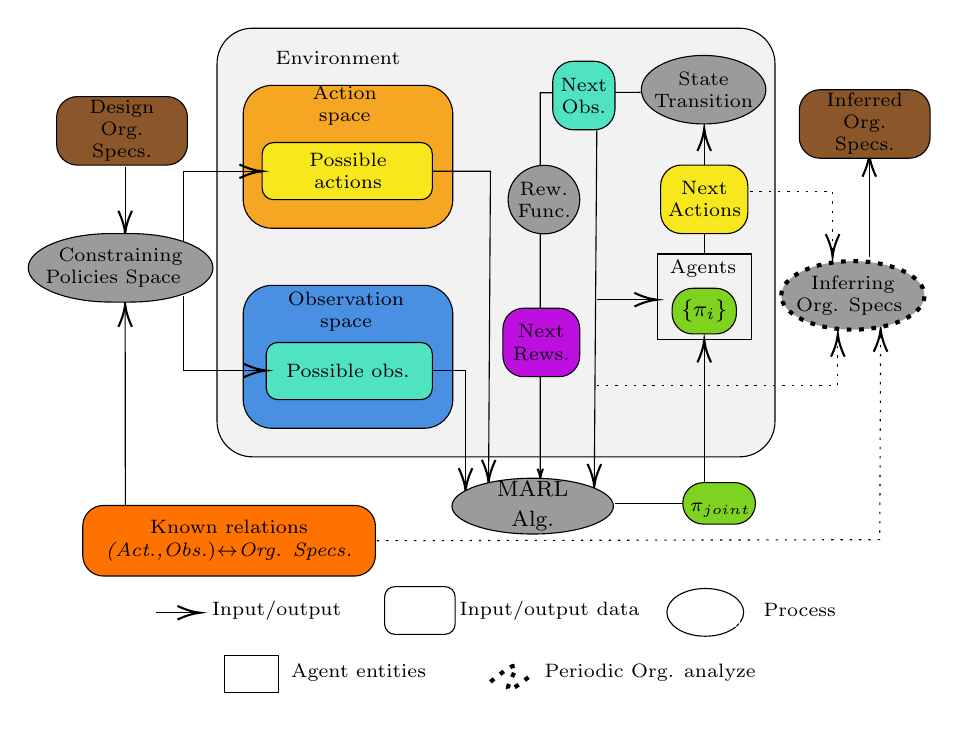
\begin{tikzpicture}[x=0.75pt,y=0.75pt,yscale=-1,xscale=1]
%uncomment if require: \path (0,1124); %set diagram left start at 0, and has height of 1124

%Shape: Rectangle [id:dp9937795244635512] 
\draw  [fill={rgb, 255:red, 242; green, 242; blue, 242 }  ,fill opacity=1 ] (108.97,721) .. controls (108.97,711.61) and (116.58,704) .. (125.97,704) -- (360.78,704) .. controls (370.17,704) and (377.78,711.61) .. (377.78,721) -- (377.78,893.49) .. controls (377.78,902.88) and (370.17,910.49) .. (360.78,910.49) -- (125.97,910.49) .. controls (116.58,910.49) and (108.97,902.88) .. (108.97,893.49) -- cycle ;
%Straight Lines [id:da6518751125509914] 
\draw    (335.62,932.92) -- (300.7,932.92) ;
%Straight Lines [id:da34207082497735786] 
\draw    (313,734.86) -- (264.7,735.09) -- (264.7,918.61) ;
\draw [shift={(264.7,920.61)}, rotate = 270] [color={rgb, 255:red, 0; green, 0; blue, 0 }  ][line width=0.75]    (4.37,-1.32) .. controls (2.78,-0.56) and (1.32,-0.12) .. (0,0) .. controls (1.32,0.12) and (2.78,0.56) .. (4.37,1.32)   ;
%Straight Lines [id:da9417034389402881] 
\draw    (343.7,754.18) -- (343.7,812.75) ;
\draw [shift={(343.7,752.18)}, rotate = 90] [color={rgb, 255:red, 0; green, 0; blue, 0 }  ][line width=0.75]    (10.93,-3.29) .. controls (6.95,-1.4) and (3.31,-0.3) .. (0,0) .. controls (3.31,0.3) and (6.95,1.4) .. (10.93,3.29)   ;
%Straight Lines [id:da4463435210078386] 
\draw    (343.7,922.88) -- (343.7,856.05) ;
\draw [shift={(343.7,854.05)}, rotate = 90] [color={rgb, 255:red, 0; green, 0; blue, 0 }  ][line width=0.75]    (10.93,-3.29) .. controls (6.95,-1.4) and (3.31,-0.3) .. (0,0) .. controls (3.31,0.3) and (6.95,1.4) .. (10.93,3.29)   ;
%Straight Lines [id:da8247669117759437] 
\draw    (291.96,834.78) -- (300.52,834.78) -- (318.99,834.78) ;
\draw [shift={(320.99,834.78)}, rotate = 180] [color={rgb, 255:red, 0; green, 0; blue, 0 }  ][line width=0.75]    (10.93,-3.29) .. controls (6.95,-1.4) and (3.31,-0.3) .. (0,0) .. controls (3.31,0.3) and (6.95,1.4) .. (10.93,3.29)   ;
%Rounded Rect [id:dp13052707912371297] 
\draw  [fill={rgb, 255:red, 245; green, 166; blue, 35 }  ,fill opacity=1 ] (121.59,745.3) .. controls (121.59,737.7) and (127.75,731.53) .. (135.35,731.53) -- (208.78,731.53) .. controls (216.39,731.53) and (222.55,737.7) .. (222.55,745.3) -- (222.55,786.6) .. controls (222.55,794.2) and (216.39,800.36) .. (208.78,800.36) -- (135.35,800.36) .. controls (127.75,800.36) and (121.59,794.2) .. (121.59,786.6) -- cycle ;
%Rounded Rect [id:dp7026077814365836] 
\draw  [fill={rgb, 255:red, 74; green, 144; blue, 226 }  ,fill opacity=1 ] (121.59,841.66) .. controls (121.59,834.06) and (127.75,827.89) .. (135.35,827.89) -- (208.78,827.89) .. controls (216.39,827.89) and (222.55,834.06) .. (222.55,841.66) -- (222.55,882.96) .. controls (222.55,890.56) and (216.39,896.72) .. (208.78,896.72) -- (135.35,896.72) .. controls (127.75,896.72) and (121.59,890.56) .. (121.59,882.96) -- cycle ;
%Rounded Rect [id:dp7429651229296941] 
\draw  [fill={rgb, 255:red, 248; green, 231; blue, 28 }  ,fill opacity=1 ] (130.7,764.57) .. controls (130.7,761.53) and (133.17,759.06) .. (136.21,759.06) -- (207.2,759.06) .. controls (210.24,759.06) and (212.7,761.53) .. (212.7,764.57) -- (212.7,781.09) .. controls (212.7,784.13) and (210.24,786.6) .. (207.2,786.6) -- (136.21,786.6) .. controls (133.17,786.6) and (130.7,784.13) .. (130.7,781.09) -- cycle ;
%Rounded Rect [id:dp2626666197665244] 
\draw  [fill={rgb, 255:red, 80; green, 227; blue, 194 }  ,fill opacity=1 ] (132.7,860.9) .. controls (132.7,857.86) and (135.17,855.39) .. (138.21,855.39) -- (207.2,855.39) .. controls (210.24,855.39) and (212.7,857.86) .. (212.7,860.9) -- (212.7,877.42) .. controls (212.7,880.46) and (210.24,882.92) .. (207.2,882.92) -- (138.21,882.92) .. controls (135.17,882.92) and (132.7,880.46) .. (132.7,877.42) -- cycle ;
%Straight Lines [id:da37906510942957117] 
\draw    (291.96,750.8) -- (290.72,922.92) ;
\draw [shift={(290.7,924.92)}, rotate = 270.41] [color={rgb, 255:red, 0; green, 0; blue, 0 }  ][line width=0.75]    (10.93,-3.29) .. controls (6.95,-1.4) and (3.31,-0.3) .. (0,0) .. controls (3.31,0.3) and (6.95,1.4) .. (10.93,3.29)   ;
%Straight Lines [id:da8878827995944159] 
\draw  [dash pattern={on 0.84pt off 2.51pt}]  (361.37,782.47) -- (405.54,782.47) -- (405.54,812.13) ;
\draw [shift={(405.54,814.13)}, rotate = 270] [color={rgb, 255:red, 0; green, 0; blue, 0 }  ][line width=0.75]    (10.93,-3.29) .. controls (6.95,-1.4) and (3.31,-0.3) .. (0,0) .. controls (3.31,0.3) and (6.95,1.4) .. (10.93,3.29)   ;
%Straight Lines [id:da8073435187842593] 
\draw  [dash pattern={on 0.84pt off 2.51pt}]  (291.96,876.08) -- (408.07,876.08) -- (408.07,853.3) ;
\draw [shift={(408.07,851.3)}, rotate = 90] [color={rgb, 255:red, 0; green, 0; blue, 0 }  ][line width=0.75]    (10.93,-3.29) .. controls (6.95,-1.4) and (3.31,-0.3) .. (0,0) .. controls (3.31,0.3) and (6.95,1.4) .. (10.93,3.29)   ;
%Straight Lines [id:da9521506867066192] 
\draw    (137.99,947.66) -- (64.8,947.66) -- (64.7,838.92) ;
\draw [shift={(64.7,836.92)}, rotate = 89.95] [color={rgb, 255:red, 0; green, 0; blue, 0 }  ][line width=0.75]    (10.93,-3.29) .. controls (6.95,-1.4) and (3.31,-0.3) .. (0,0) .. controls (3.31,0.3) and (6.95,1.4) .. (10.93,3.29)   ;
%Straight Lines [id:da8173351196218479] 
\draw  [dash pattern={on 0.84pt off 2.51pt}]  (177.06,950.92) -- (428.26,950.41) -- (428.69,850.92) ;
\draw [shift={(428.7,848.92)}, rotate = 90.25] [color={rgb, 255:red, 0; green, 0; blue, 0 }  ][line width=0.75]    (10.93,-3.29) .. controls (6.95,-1.4) and (3.31,-0.3) .. (0,0) .. controls (3.31,0.3) and (6.95,1.4) .. (10.93,3.29)   ;
%Straight Lines [id:da6053298376683525] 
\draw    (64.7,770.92) -- (64.7,800.92) ;
\draw [shift={(64.7,802.92)}, rotate = 270] [color={rgb, 255:red, 0; green, 0; blue, 0 }  ][line width=0.75]    (10.93,-3.29) .. controls (6.95,-1.4) and (3.31,-0.3) .. (0,0) .. controls (3.31,0.3) and (6.95,1.4) .. (10.93,3.29)   ;
%Straight Lines [id:da8641416537329594] 
\draw    (423.21,814.13) -- (423.21,766.57) ;
\draw [shift={(423.21,764.57)}, rotate = 90] [color={rgb, 255:red, 0; green, 0; blue, 0 }  ][line width=0.75]    (10.93,-3.29) .. controls (6.95,-1.4) and (3.31,-0.3) .. (0,0) .. controls (3.31,0.3) and (6.95,1.4) .. (10.93,3.29)   ;
%Shape: Rectangle [id:dp009612592743657444] 
\draw   (320.99,812.75) -- (366.42,812.75) -- (366.42,854.05) -- (320.99,854.05) -- cycle ;
%Shape: Boxed Line [id:dp9105440631185389] 
\draw    (79.7,985.61) -- (98.84,985.61) ;
\draw [shift={(100.84,985.61)}, rotate = 180] [color={rgb, 255:red, 0; green, 0; blue, 0 }  ][line width=0.75]    (10.93,-3.29) .. controls (6.95,-1.4) and (3.31,-0.3) .. (0,0) .. controls (3.31,0.3) and (6.95,1.4) .. (10.93,3.29)   ;
%Shape: Rectangle [id:dp18940852352890292] 
\draw   (112.7,1006.17) -- (138.7,1006.17) -- (138.7,1023.94) -- (112.7,1023.94) -- cycle ;
%Curve Lines [id:da6070406744312455] 
\draw [line width=1.5]  [dash pattern={on 1.69pt off 2.76pt}]  (240.7,1018.92) .. controls (271.17,993.71) and (230.78,1040.06) .. (261.24,1014.84) ;
%Straight Lines [id:da04181106466856366] 
\draw    (92.7,806.92) -- (92.7,772.92) -- (128.7,772.92) ;
\draw [shift={(130.7,772.92)}, rotate = 180] [color={rgb, 255:red, 0; green, 0; blue, 0 }  ][line width=0.75]    (10.93,-3.29) .. controls (6.95,-1.4) and (3.31,-0.3) .. (0,0) .. controls (3.31,0.3) and (6.95,1.4) .. (10.93,3.29)   ;
%Straight Lines [id:da5269327271789521] 
\draw    (92.7,832.92) -- (92.7,868.92) -- (130.7,868.92) ;
\draw [shift={(132.7,868.92)}, rotate = 180] [color={rgb, 255:red, 0; green, 0; blue, 0 }  ][line width=0.75]    (10.93,-3.29) .. controls (6.95,-1.4) and (3.31,-0.3) .. (0,0) .. controls (3.31,0.3) and (6.95,1.4) .. (10.93,3.29)   ;
%Straight Lines [id:da8384029096649059] 
\draw    (228.7,924.92) -- (228.7,868.92) -- (212.7,868.92) ;
\draw [shift={(228.7,926.92)}, rotate = 270] [color={rgb, 255:red, 0; green, 0; blue, 0 }  ][line width=0.75]    (10.93,-3.29) .. controls (6.95,-1.4) and (3.31,-0.3) .. (0,0) .. controls (3.31,0.3) and (6.95,1.4) .. (10.93,3.29)   ;
%Straight Lines [id:da8549749304566603] 
\draw    (212.7,772.92) -- (240.7,772.92) -- (239.8,920.92) ;
\draw [shift={(239.79,922.92)}, rotate = 270.35] [color={rgb, 255:red, 0; green, 0; blue, 0 }  ][line width=0.75]    (10.93,-3.29) .. controls (6.95,-1.4) and (3.31,-0.3) .. (0,0) .. controls (3.31,0.3) and (6.95,1.4) .. (10.93,3.29)   ;

% Text Node
\draw (177.2,1014.42) node  [font=\small] [align=left] {{\scriptsize Agent entities}};
% Text Node
\draw (317.7,1014.42) node  [font=\small] [align=left] {{\scriptsize Periodic Org. analyze}};
% Text Node
\draw    (189.7,978.02) .. controls (189.7,975.26) and (191.94,973.02) .. (194.7,973.02) -- (218.7,973.02) .. controls (221.46,973.02) and (223.7,975.26) .. (223.7,978.02) -- (223.7,991.02) .. controls (223.7,993.78) and (221.46,996.02) .. (218.7,996.02) -- (194.7,996.02) .. controls (191.94,996.02) and (189.7,993.78) .. (189.7,991.02) -- cycle  ;
\draw (206.7,984.52) node  [font=\small] [align=left] {\begin{minipage}[lt]{20.08pt}\setlength\topsep{0pt}
\begin{center}
\textcolor[rgb]{1,1,1}{{\tiny assaaaa}}
\end{center}

\end{minipage}};
% Text Node
\draw (269.2,984.42) node  [font=\small] [align=left] {{\scriptsize Input/output data}};
% Text Node
\draw (137.7,984.42) node  [font=\small] [align=left] {{\scriptsize Input/output}};
% Text Node
\draw    (325.7,985.42) .. controls (325.7,979.07) and (333.98,973.92) .. (344.2,973.92) .. controls (354.42,973.92) and (362.7,979.07) .. (362.7,985.42) .. controls (362.7,991.77) and (354.42,996.92) .. (344.2,996.92) .. controls (333.98,996.92) and (325.7,991.77) .. (325.7,985.42) -- cycle  ;
\draw (344.2,985.42) node  [font=\small] [align=left] {\begin{minipage}[lt]{22.12pt}\setlength\topsep{0pt}
\begin{center}
\textcolor[rgb]{1,1,1}{{\tiny aassssaa}}
\end{center}

\end{minipage}};
% Text Node
\draw (389.7,984.42) node  [font=\small] [align=left] {{\scriptsize Process}};
% Text Node
\draw  [fill={rgb, 255:red, 139; green, 87; blue, 42 }  ,fill opacity=1 ]  (31.7,746.92) .. controls (31.7,741.4) and (36.18,736.92) .. (41.7,736.92) -- (84.7,736.92) .. controls (90.22,736.92) and (94.7,741.4) .. (94.7,746.92) -- (94.7,759.92) .. controls (94.7,765.45) and (90.22,769.92) .. (84.7,769.92) -- (41.7,769.92) .. controls (36.18,769.92) and (31.7,765.45) .. (31.7,759.92) -- cycle  ;
\draw (63.2,753.42) node  [font=\scriptsize] [align=left] {\begin{minipage}[lt]{40.43pt}\setlength\topsep{0pt}
\begin{center}
Design\\Org. Specs.
\end{center}

\end{minipage}};
% Text Node
\draw  [fill={rgb, 255:red, 155; green, 155; blue, 155 }  ,fill opacity=1 ]  (249.21,786.55) .. controls (249.21,777.43) and (256.94,770.05) .. (266.46,770.05) .. controls (275.99,770.05) and (283.72,777.43) .. (283.72,786.55) .. controls (283.72,795.66) and (275.99,803.05) .. (266.46,803.05) .. controls (256.94,803.05) and (249.21,795.66) .. (249.21,786.55) -- cycle  ;
\draw (266.46,786.55) node  [font=\scriptsize,xslant=-0.02] [align=left] {\begin{minipage}[lt]{20.58pt}\setlength\topsep{0pt}
\begin{center}
Rew.\\Func.
\end{center}

\end{minipage}};
% Text Node
\draw (165.76,716.05) node  [font=\scriptsize] [align=left] {\begin{minipage}[lt]{42.81pt}\setlength\topsep{0pt}
\begin{center}
Environment
\end{center}

\end{minipage}};
% Text Node
\draw (170.49,741.51) node  [font=\scriptsize] [align=left] {\begin{minipage}[lt]{43.61pt}\setlength\topsep{0pt}
\begin{center}
Action space
\end{center}

\end{minipage}};
% Text Node
\draw (171.12,840.63) node  [font=\scriptsize] [align=left] {\begin{minipage}[lt]{62.26pt}\setlength\topsep{0pt}
\begin{center}
Observation space
\end{center}

\end{minipage}};
% Text Node
\draw (172.07,772.83) node  [font=\scriptsize] [align=left] {\begin{minipage}[lt]{54.32pt}\setlength\topsep{0pt}
\begin{center}
Possible actions
\end{center}

\end{minipage}};
% Text Node
\draw (172.07,869.19) node  [font=\scriptsize] [align=left] {\begin{minipage}[lt]{45.19pt}\setlength\topsep{0pt}
\begin{center}
Possible obs.
\end{center}

\end{minipage}};
% Text Node
\draw  [fill={rgb, 255:red, 155; green, 155; blue, 155 }  ,fill opacity=1 ]  (261.04, 934.24) circle [x radius= 38.89, y radius= 13.44]   ;
\draw (261.04,934.24) node  [font=\small] [align=left] {\begin{minipage}[lt]{37.13pt}\setlength\topsep{0pt}
\begin{center}
{\footnotesize MARL Alg.}
\end{center}

\end{minipage}};
% Text Node
\draw  [fill={rgb, 255:red, 126; green, 211; blue, 33 }  ,fill opacity=1 ]  (333.36,932.92) .. controls (333.36,927.4) and (337.84,922.92) .. (343.36,922.92) -- (358.36,922.92) .. controls (363.88,922.92) and (368.36,927.4) .. (368.36,932.92) .. controls (368.36,938.45) and (363.88,942.92) .. (358.36,942.92) -- (343.36,942.92) .. controls (337.84,942.92) and (333.36,938.45) .. (333.36,932.92) -- cycle  ;
\draw (350.86,932.92) node  [font=\scriptsize] [align=left] {\begin{minipage}[lt]{20.95pt}\setlength\topsep{0pt}
\begin{center}
$\displaystyle \pi _{joint}$
\end{center}

\end{minipage}};
% Text Node
\draw  [fill={rgb, 255:red, 155; green, 155; blue, 155 }  ,fill opacity=1 ]  (313.39,733.6) .. controls (313.39,724.48) and (326.82,717.1) .. (343.39,717.1) .. controls (359.96,717.1) and (373.39,724.48) .. (373.39,733.6) .. controls (373.39,742.71) and (359.96,750.1) .. (343.39,750.1) .. controls (326.82,750.1) and (313.39,742.71) .. (313.39,733.6) -- cycle  ;
\draw (343.39,733.6) node  [font=\scriptsize] [align=left] {\begin{minipage}[lt]{37.77pt}\setlength\topsep{0pt}
\begin{center}
State\\Transition \ 
\end{center}

\end{minipage}};
% Text Node
\draw  [fill={rgb, 255:red, 189; green, 16; blue, 224 }  ,fill opacity=1 ]  (246.7,848.88) .. controls (246.7,843.35) and (251.18,838.88) .. (256.7,838.88) -- (273.7,838.88) .. controls (279.22,838.88) and (283.7,843.35) .. (283.7,848.88) -- (283.7,861.88) .. controls (283.7,867.4) and (279.22,871.88) .. (273.7,871.88) -- (256.7,871.88) .. controls (251.18,871.88) and (246.7,867.4) .. (246.7,861.88) -- cycle  ;
\draw (265.2,855.38) node  [font=\scriptsize] [align=left] {\begin{minipage}[lt]{22.57pt}\setlength\topsep{0pt}
\begin{center}
Next\\Rews.
\end{center}

\end{minipage}};
% Text Node
\draw  [fill={rgb, 255:red, 255; green, 114; blue, 0 }  ,fill opacity=1 ]  (44.27,943.92) .. controls (44.27,938.4) and (48.75,933.92) .. (54.27,933.92) -- (175.27,933.92) .. controls (180.79,933.92) and (185.27,938.4) .. (185.27,943.92) -- (185.27,957.92) .. controls (185.27,963.45) and (180.79,967.92) .. (175.27,967.92) -- (54.27,967.92) .. controls (48.75,967.92) and (44.27,963.45) .. (44.27,957.92) -- cycle  ;
\draw (114.77,950.92) node  [font=\scriptsize] [align=left] {\begin{minipage}[lt]{93.15pt}\setlength\topsep{0pt}
\begin{center}
Known relations\\\textit{(Act.,Obs.})$\displaystyle \leftrightarrow $\textit{Org. Specs.}
\end{center}

\end{minipage}};
% Text Node
\draw  [fill={rgb, 255:red, 155; green, 155; blue, 155 }  ,fill opacity=1 ]  (18,819.42) .. controls (18,810.31) and (35.91,802.92) .. (58,802.92) -- (67,802.92) .. controls (89.09,802.92) and (107,810.31) .. (107,819.42) .. controls (107,828.54) and (89.09,835.92) .. (67,835.92) -- (58,835.92) .. controls (35.91,835.92) and (18,828.54) .. (18,819.42) -- cycle  ;
\draw (62.5,819.42) node  [font=\scriptsize] [align=left] {\begin{minipage}[lt]{57.49pt}\setlength\topsep{0pt}
\begin{center}
Constraining\\Policies Space \ \ \ 
\end{center}

\end{minipage}};
% Text Node
\draw  [fill={rgb, 255:red, 80; green, 227; blue, 194 }  ,fill opacity=1 ]  (270.7,729.92) .. controls (270.7,724.4) and (275.18,719.92) .. (280.7,719.92) -- (290.7,719.92) .. controls (296.22,719.92) and (300.7,724.4) .. (300.7,729.92) -- (300.7,742.92) .. controls (300.7,748.45) and (296.22,752.92) .. (290.7,752.92) -- (280.7,752.92) .. controls (275.18,752.92) and (270.7,748.45) .. (270.7,742.92) -- cycle  ;
\draw (285.7,736.42) node  [font=\scriptsize] [align=left] {\begin{minipage}[lt]{17.81pt}\setlength\topsep{0pt}
\begin{center}
Next\\Obs.
\end{center}

\end{minipage}};
% Text Node
\draw (343.14,819.98) node  [font=\scriptsize] [align=left] {\begin{minipage}[lt]{24.96pt}\setlength\topsep{0pt}
\begin{center}
Agents
\end{center}

\end{minipage}};
% Text Node
\draw  [fill={rgb, 255:red, 126; green, 211; blue, 33 }  ,fill opacity=1 ]  (328.2,839.28) .. controls (328.2,833.76) and (332.68,829.28) .. (338.2,829.28) -- (349.2,829.28) .. controls (354.73,829.28) and (359.2,833.76) .. (359.2,839.28) -- (359.2,841.28) .. controls (359.2,846.81) and (354.73,851.28) .. (349.2,851.28) -- (338.2,851.28) .. controls (332.68,851.28) and (328.2,846.81) .. (328.2,841.28) -- cycle  ;
\draw (343.7,840.28) node  [font=\footnotesize] [align=left] {\begin{minipage}[lt]{18.45pt}\setlength\topsep{0pt}
\begin{center}
$\displaystyle \{\pi _{i}\}$
\end{center}

\end{minipage}};
% Text Node
\draw  [fill={rgb, 255:red, 248; green, 231; blue, 28 }  ,fill opacity=1 ]  (322.7,779.92) .. controls (322.7,774.4) and (327.18,769.92) .. (332.7,769.92) -- (354.7,769.92) .. controls (360.22,769.92) and (364.7,774.4) .. (364.7,779.92) -- (364.7,792.92) .. controls (364.7,798.45) and (360.22,802.92) .. (354.7,802.92) -- (332.7,802.92) .. controls (327.18,802.92) and (322.7,798.45) .. (322.7,792.92) -- cycle  ;
\draw (343.7,786.42) node  [font=\scriptsize] [align=left] {\begin{minipage}[lt]{26.14pt}\setlength\topsep{0pt}
\begin{center}
Next\\Actions
\end{center}

\end{minipage}};
% Text Node
\draw  [color={rgb, 255:red, 0; green, 0; blue, 0 }  ,draw opacity=1 ][fill={rgb, 255:red, 155; green, 155; blue, 155 }  ,fill opacity=1 ][dash pattern={on 1.69pt off 2.76pt}][line width=1.5]   (380.82,832.71) .. controls (380.82,823.6) and (396.27,816.21) .. (415.32,816.21) .. controls (434.38,816.21) and (449.82,823.6) .. (449.82,832.71) .. controls (449.82,841.82) and (434.38,849.21) .. (415.32,849.21) .. controls (396.27,849.21) and (380.82,841.82) .. (380.82,832.71) -- cycle  ;
\draw (415.32,832.71) node  [font=\scriptsize] [align=left] {\begin{minipage}[lt]{44.39pt}\setlength\topsep{0pt}
\begin{center}
Inferring\\Org. Specs \ \ 
\end{center}

\end{minipage}};
% Text Node
\draw  [fill={rgb, 255:red, 139; green, 87; blue, 42 }  ,fill opacity=1 ]  (389.5,743.62) .. controls (389.5,738.09) and (393.98,733.62) .. (399.5,733.62) -- (442.5,733.62) .. controls (448.02,733.62) and (452.5,738.09) .. (452.5,743.62) -- (452.5,756.62) .. controls (452.5,762.14) and (448.02,766.62) .. (442.5,766.62) -- (399.5,766.62) .. controls (393.98,766.62) and (389.5,762.14) .. (389.5,756.62) -- cycle  ;
\draw (421,750.12) node  [font=\scriptsize] [align=left] {\begin{minipage}[lt]{40.43pt}\setlength\topsep{0pt}
\begin{center}
Inferred\\Org. Specs.
\end{center}

\end{minipage}};


\end{tikzpicture}
    \caption{A summary view of the PRAHOM process}
    \label{fig:prahom_process}
\end{figure}

% \RestyleAlgo{ruled}
% \SetKwComment{Comment}{// }{}

% \begin{algorithm}[hbt!]
%     \caption{Partial Relations with Agent History and Organization Model (PRAHOM)}\label{alg:prahom}

%     \KwData{$d$, the Dec-POMDP to solve}
%     \KwData{$ep_{max} \in \mathbb{N}$, the maximum number of episodes}
%     \KwData{$step_{max} \in \mathbb{N}$, the maximum number of steps per episodes}
%     \KwData{$s \in \mathbb{R}$, the cumulative reward expectancy}
%     \KwData{$\pi_{joint}$, the joint-policies to be trained}
%     \KwData{$os_{init}$, the design specifications to respect}
%     \KwData{$Solv$, a MARL algorithm updating policies to solve a Dec-POMDP}

%     \KwResult{$(s\pi_{joint,s,i} \in S\Pi_{joint,s,i}, os_{s,i} \in OS_{s,i})$, the sub-optimal policies associated organization specifications}

%     $s\pi_{joint,s,i} = PRAHOM-osh-training(s,i)$

%     $os_{s,i} = PRAHOM-hos(s\pi_{joint,s,i})$

% \end{algorithm}

\paragraph{\textbf{Inferring Organizational Specifications}}

Rather than using joint-policies directly, we use the joint-histories since they may be built with observed resulting actions when observations are received during a series of test episodes. Indeed, for a given policy $\pi \in \Pi$, the associated history is by definition $h \in h_{joint} = \langle(\omega_k,a_k) | k \in \mathbb{N}\rangle$ and the $(\omega_k,a_k) \in \pi$.
Then, due to the difficulty of inferring information related to organizational specifications, it is possible to associate each observation or action with organization specifications as a \textquote{many to many} relation. It sets up a first frame for identifying organizational specifications in histories. We address that problem in the remainder of this section.

One can define some relations between $\mathcal{M}OISE^+$ specifications and joint-histories. Their premises come from noticing some specifications in the $\mathcal{M}OISE^+$ organizational model can be mapped to subsets of actions from a single suboptimal joint-policy.
From these relations, it is possible to use empirical or statistical approaches to infer organizational specifications out of joint-histories. Below we informally describe key points for understanding that process.

As we have only one group, we do not consider the inter-links and inter-compatibilities. Additionally, as a simplification, we consider only one social scheme.
First, we look at the individual level by trying to figure out the roles, links, sub-groups, individual goals, missions, and plans played by agents by sampling history subsequences $h \in H$ and comparing with known history subsequences whose we know the associated role via the established relations.

After analyzing several joint-policies, we try to reinforce a global view of the goals, missions, plans, and the knowledge of the mission to the goal; with the partially inferred information at the individual level.
In the end, our process tries to synthesize the knowledge inferred until having a better view of the agent cardinality per sub-group, the agent cardinality for each mission, the role cardinality, the compatibilities between roles, the permissions, and obligations.

\paragraph{\textbf{Constraining Policies Space}}

We consider a given MARL algorithm that iteratively converges towards a joint-policy so that each agent's policy is updated at each step until a finite horizon.
We favored the Proximal Policy Optimization for its proven effectiveness in cooperative multi-agent environments without the need for domain-specific algorithmic modifications or architectures~\cite{Yu2022}.
To constrain the possible joint-policies to the ones satisfying the design organizational specifications $os_{init}$, we propose to constrain the action and observation sets for each agent according to $os_{init}$ at each step. Ultimately, it constrains an agent to a role by forbidding actions related to other roles.

First, we use the established relations between organizational specifications and action-observation couples, to determine the authorized or forbidden actions playable by agents at each step.
Then, it first computes the authorized actions set $A_{step}$ according to the current history $h_{joint,i}$. Then, an action is chosen among authorized actions. That action $a_{step} \in A_{step}$ is added in history to be used for updating the agent's policy in the next step. Then, the MARL algorithm updates the joint-policy hence the agents' policies with the current action and observation.
Finally, an analysis of the current suboptimal joint-policy $\pi_{joint}$ satisfying $os_{init}$ is triggered periodically. It enables iteratively improving the efficiency of joint-policies and the accuracy of the inferred organizational specifications.
We can note the restriction implied by $os_{init}$ in the possible joint-policies might prevent the MARL algorithm from finding a joint-policy that satisfies the minimal expected cumulative reward defined by the designer.

\subsection{Engineering tool}

PettingZoo is a library that offers a standardized API that simplifies the development of environments with agents and facilitates the application of MARL algorithms.
We developed \emph{PRAHOM PettingZoo Wrapper}\label{PettingZoo-wrapper}, a tool to help automate the setting up of \emph{PRAHOM} for a given PettingZoo environment.
It is a \emph{PoC} linking joint-histories with $\mathcal{M}OISE^+$ specifications to provide functions to infer raw organizational specifications or constrain the training. %During training, actions are masked/fostered to agents regarding the given organizational specifications as constraints.
%
\begin{lstlisting}[language=Python, caption=PRAHOM PettingZoo Wrapper basic use, label={lst:wrapper_basic_use}]
from omarl_experiments import prahom_wrapper
env=PettingZoo_env.parallel_env(render_mode="human")
specs_to_hist={"structural_specifications":{"roles":{"follower":{"23":41,"14":[74,0]}}...},"functional_specifications":{"links":{"(leader,follower,aut)":".*14.*?89"}...}...}
policy_specs_constr={"agent_0":{"structural_specifications":"roles":["follower"]}}
env=prahom_wrapper(env,action_to_specs,training_specs)
env.train("default_PPO")
trained_specs,agent_to_specs=env.prahom_specs()
\end{lstlisting}
%
In \autoref{lst:wrapper_basic_use}, we detailed a basic use of the wrapper to augment a PettingZoo environment (l. 5) with known relations between histories and organizational specifications (l. 3) and the design constraints agents are to satisfy (l. 4).
During training, \textquote{"agent\_0"} is constrained to role \textquote{follower} so all of its actions must be chosen regarding the relations between organizational specifications and expected histories (or shortened histories expressions).
After training, \emph{PRAHOM PettingZoo Wrapper} infers organizational specifications from joint-histories in 5 episodes, and the agents' instantiation for each one (l. 7).

This process first uses known relations between histories and organizational specifications (l. 3): an agent's history that contains the observation $14$ (\textquote{order received}) and the action $74$ (\textquote{apply order}) or $0$ (\textquote{do nothing}), is a \textquote{follower}. Similarly, history can be linked to organizational specifications with regular expressions such as for \emph{links} (l.3).
Then, it generalizes several joint-histories as new organizational specifications relying on their respective general definition.
%
For instance, a role is thought to be inferred by measuring similarity between histories in several ways: sequence clustering (with a dendrogram); K-nearest neighbors (with PCA of histories); statistical analysis (specially action frequency in various visualizations); etc.
%
Techniques are also used to infer goals: frequency analysis of common observations of agents with the same role; analysis of threshold states triggering an improvement of the reward (with a state transition graph).

From the roles and goals obtained, an empiric approach allows inferring the other organizational specifications such as compatibilities, permissions and obligations.
Due to that empiric approach and the specific scope of the techniques, results may be incomplete or noisy. Yet, since results are compliant with $\mathcal{M}OISE^+$, it is possible to use them in MAS design methods in light of the identified organizational specifications.

% We start defining actions with known specifications Focusing of the "lead adversary", we have:

% "observations": [self_vel, self_pos, landmark_rel_positions, other_agent_rel_positions, other_agent_velocities, leader_comm]
% "actions": [say_0, say_1, say_2, say_3] X [no_action, move_left, move_right, move_down, move_up]

% =============

% \subsection{Premises for AOMEA's theoretical core}

% - Organizational oriented MARL: a general research study focusing in integrating the organization in MARL at several aspects
% - DMO (Dec-POMDP MOISE+ OMARL): a class of algorithm falling into OMARL purposes that use MOISE+ as organizational model and Dec-POMDP as a MARL model
% - PRAHOM (Partial Relations with Agent History and Organization Model): a DMO algorithm that allows both getting the organizational specifications out of trained agents; and driving their training to satisfy extra design organizational specifications as constraints.

% \subsection{AOMEA for engineering}

% - We proposed PRAHOM (Partial Relations with Agent History and Organization Model): an algorithm that allows both getting the organizational specifications out of trained agents; and driving their training to satisfy extra design organizational specifications as constraints.
% - [Algo PRAHOM...]

% - We developped PRAHOM as a PettingZoo-wrapper to help in applying the proposed MAS design approach...
% - [Lien vers dépôt GitHub]
% - Description des fonctionalités

% - The general approach workflow follows:
% 1) Reproducing target environment in simulation
% 2) Defining the reward function so agents aim to achieve the goals
% 3) Adding agents to be trained to solve the previously defined problem
% 4) Launching the training in simulation with PRAHOM
% 5) Getting the raw organizational specifications with PRAHOM
% 6) Curating these to produce a safe MAS model
% 7) Using that model to implement a proper MAS
% 8) Check viability and requirements respect in simulation
% 9) Deploy that MAS in the target system

% \begin{itemize}
%     \item Questions at the Multi-Agent System level (system-centric approach)
%           \begin{itemize}
%               \item Number of agents, what heterogeneity?
%               \item What is the common medium (Environment) shared by the agents?
%               \item What communication mechanisms are available to agents?
%               \item What are the communication languages, ontologies, interaction protocols used by the agents?
%               \item What is the organization within which the agents operate? How is it established?
%               \item How do the agents coordinate their actions? How to ensure coherent operation?
%           \end{itemize}

%     \item Agent level questions (agent-centered approach)
%           \begin{itemize}
%               \item What does an agent represent? What actions should be encapsulated in an agent?
%               \item How do agents represent the environment and organization in which they operate?
%               \item How do agents handle interactions with other agents?
%               \item What is the internal structure of the agents?
%           \end{itemize}
% \end{itemize}

% ====================================================================================================






\section{Evaluation in cooperative game environments}

% Evaluation
%     In order to verify and demonstrate the approach, is applied on the following case study.
% 	Case study


In order to assess AOMEA, we considered using \emph{PRAHOM} in available simulated environments made up of agents that have to achieve a goal with the best performance through various collective strategies whose some can be easily understood (presented in \autoref{fig:simulated_environments}).
We selected three Atari-like environments for their visual rendering is a convenient way to assess the results with manual observations\footnotemark[1].
We also considered a Cyberdefense environment as a first attempt to apply \emph{PRAHOM} in a non-visual Cyberdefense environment:

\footnotetext[1]{Additional explanation and the examples discussed using \emph{PRAHOM PettingZoo wrapper} are available at \url{https://github.com/julien6/omarl_experiments?tab=readme-ov-file\#tutorial-predator-prey-with-communication}}


\begin{itemize}
    \item \textquote{Drone swarm - 3rd CAGE Challenge}~\cite{cage_challenge_3_announcement} (CYB) consists of cyberdender agents deployed on networked drones fighting against maliciously deployed malware programs. We may expect agents to \allowbreak isolate compromised drones;
    \item \textquote{Pistonball} (PBL)~\cite{Terry2021} consists of a series of pistons to bring a ball from right to left side hence requiring neighbors' representation;
    \item \textquote{Predator-prey with communication}~\cite{Lowe2017} (PPY) consists of predators monitored by a leader to catch faster prey hence requiring hunting strategies;
    \item \textquote{Knights Archers Zombies}~\cite{Terry2021} (KAZ) consists in knights and archers learning how to kill zombies hence requiring efficient agent spatial positioning.
\end{itemize}
%
\begin{figure}[H]
    \centering
    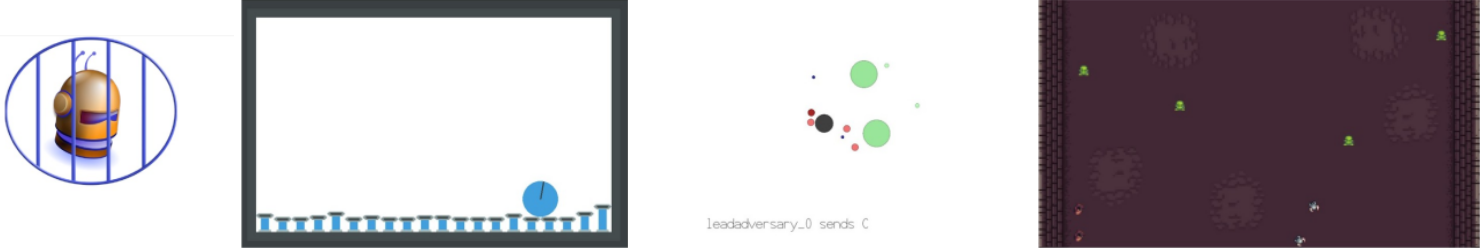
\includegraphics[width=0.8\linewidth]{figures/envs_4x1.png}
    \caption{Overview of the selected environments: CYB, PBL, PPY, and KAZ}
    \label{fig:simulated_environments}
\end{figure}
%
\noindent We applied AOMEA in three cases:
\begin{itemize}
    \item No organizational specifications (NTS): agents have to learn the most efficient collective strategies without any constraints or indications.
    \item Partially constraining organizational specifications (PTS): some constraints or indications are given to help converge faster or meet requirements.
    \item Fully constraining organizational specifications (FTS): manually crafted joint-policies are given for they are a reference regarding learned joint-policies.
\end{itemize}

\noindent Here, we do not present the details of the constraints that were given in NTS and FTS (available in Git repository\footnotemark[1]).
%
\begin{figure}[h!]
    \centering
    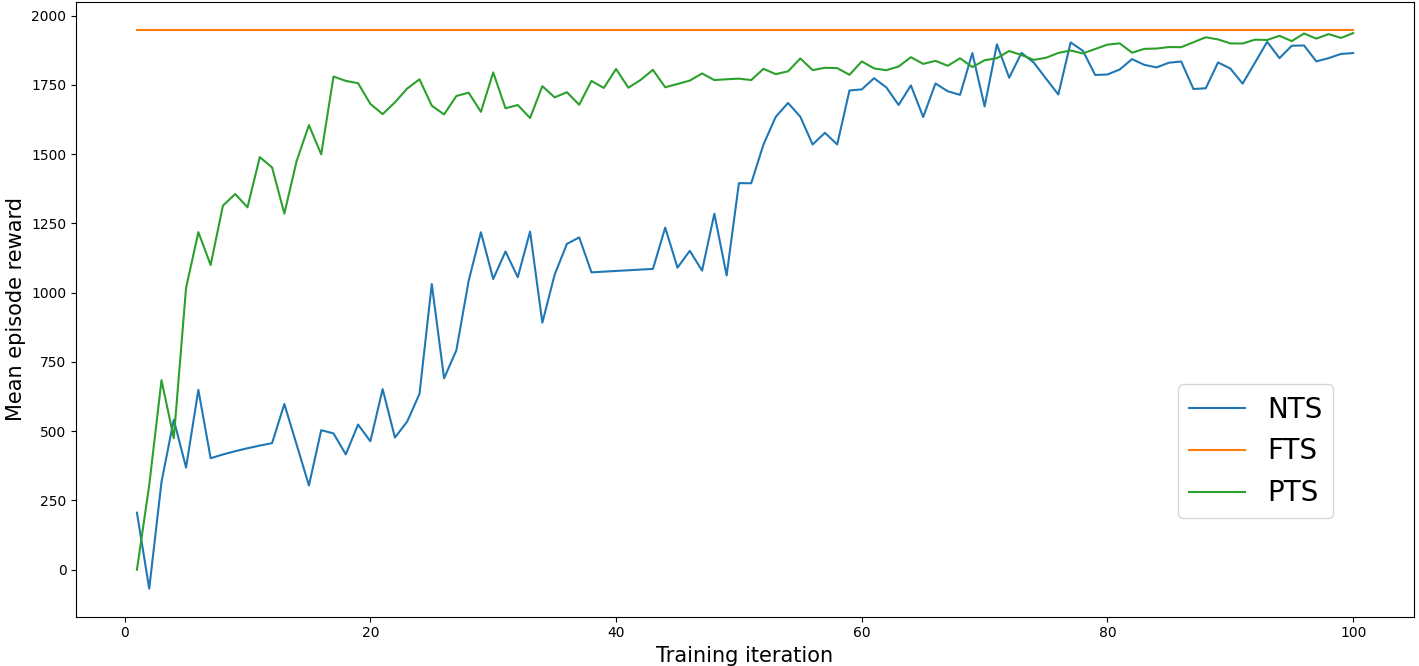
\includegraphics[width=0.8\textwidth]{figures/prahom_learning_curve.png}
    \caption{Average reward for each iteration in the PBL environment for the NTS, PTS, and FTS cases}
    \label{fig:prahom_learning_curve}
\end{figure}
%
\begin{figure}[h!]
    \centering
    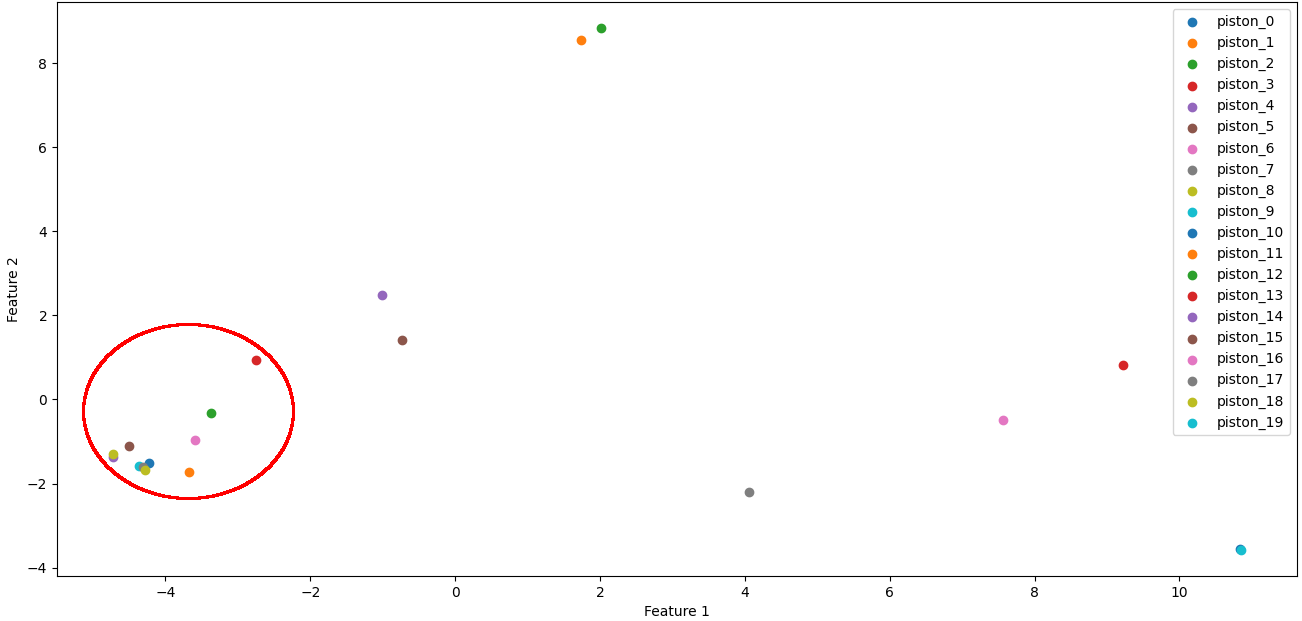
\includegraphics[width=0.8\textwidth]{figures/prahom_pca_analysis.png}
    \caption{PCA of the trained agents' histories in the PBL environment}
    \label{fig:prahom_pca_analysis}
\end{figure}
%
We evaluate the impact of \emph{PRAHOM} on the following criteria: convergence time ratios between PTS, NTS, and FTS for reaching a threshold cumulative reward. Performance stability shows how the trained agents can achieve the goal generally by assessing several environments generated with different parameters. Results are presented in Table~\ref{tab:training_AOMEA_results}.
%
\begin{table}[t!]

    \centering

    \begin{tblr}{colspec={llll},rows={m},measure=vbox,stretch=-1}

        \textbf{Environment} & \textbf{PTS/NTS} & \textbf{PTS/FTS} & \textbf{Perf. stability \\ (avg. / max)} \\

        \hline

        { PPL }
        & { 4.7 }
        & { 1.3 }
        & { 0.9 } \\

        \hline[dashed]

        { PPY }
        & { 6.3 }
        & { 2.2 }
        & { 0.78 } \\

        \hline[dashed]

        { KAZ }
        & { 4.0 }
        & { 1.1 }
        & { 0.42 } \\

        \hline[dashed]

        { CYB }
        & { 12 }
        & { 3.3 }
        & { 0.36 } \\


    \end{tblr}

    \caption{View of the AOMEA approach impact during training}

    \label{tab:training_AOMEA_results}

\end{table}

%
As a general observation, we can notice convergence time is longer for NTS than for PTS which is also longer than for FTS. As expected, the search space is decreasing, hence a shorter convergence time. For instance, we noticed a faster convergence to a sub-optimal solution in the PBL environment by providing organizational specifications as presented in \autoref{fig:prahom_learning_curve}. Although PTS converges faster than NTS to a comparable cumulative reward, NTS may outperform PTS because trained agents' policies are hand-tailored to solve the problem much more finely than the designer's organizational specifications can do. Low-performance stability in the more complex CYB environment indicates that the trained agents have difficulty finding general strategies compared to the agents in the other environments.

We also took into account the following criteria after training: roles, links, and global performance. A qualitative analysis is presented in Table~\ref{tab:trained_AOMEA_results}
%
\begin{table}[t!]

    \centering

    \begin{tblr}{colspec={llll},rows={m},measure=vbox,stretch=-1}

        \textbf{Environment} & \textbf{Roles} & \textbf{Links} & \textbf{Global performance} \\

        \hline

        { 1 }
        & {  }
        & {  } \\
        & {  } \\

        \hline[dashed]

        { 2 }
        & {  }
        & {  } \\
        & {  } \\

        \hline[dashed]

        { 3 }
        & {  }
        & {  } \\
        & {  } \\

        \hline[dashed]

        { 4 }
        & {  }
        & {  } \\
        & {  } \\

        \hline[dashed]

        { 5 }
        & {  }
        & {  } \\
        & {  } \\

    \end{tblr}

    \caption{View of the OOMARL approach impact after training}

    \label{tab:trained_OOMARL_results}

\end{table}

%
% //TODO: Moise+ schemes and comparison with expected ones
%
For the PBL environment, we can notice roles being equivalent for agents are expected to act the same. Indeed, trained agents' histories are close hence showing a common emerging role. We generate the PCA presented in \autoref{fig:prahom_pca_analysis} by expressing agents' histories as vectors containing the observation-action couples. We can notice most agents’ histories are in the left bottom zone (circled in red). It shows most pistons seem to act similarly as expected. We observe no organizational specifications except roles have been generated because agents cannot communicate. For the KAZ environment, we can notice two distinct roles: archers tend to move away from zombies, while knights tend to approach them. For the PPY environment, we can observe the output specifications indicate authority links between the leader predator and the simple predators to enable collective strategies for circling prey. Finally, the CYB environment shows communications between blue agents are indeed understood as communication links that enable isolating infiltrated drones or trying to fix and alert recently suspected drones.

For the CYB environment, we developed our custom MAS via a simple hand-crafted decision tree as preconized in AOMEA in light of the organizational specifications we curated by removing noisy results. Our approach did not suggest general roles but relevant strategy patterns have been identified. For instance, regarding links between agents' roles, we noticed that the agents sending messages frequently seem to be spotted as suspected by their neighbors. In addition, a cyber-defender agent in the communication radius of a suspected drone tends to switch off its communication and reactivate afterward. Even though these insights are few, the mean score we got with our curated MAS is about -2000 which is indeed close to the top 5 scores. This shows AOMEA to be indeed applicable to the Cyberdefense context additionally bringing safety guarantees.




\section{Conclusion}

MAS methodological works rely on the designer's knowledge to design a suited MAS organization but do not provide automatic or assisted ways to determine relevant organizational mechanisms.

MARL techniques have been successfully applied to train agents automatically to reach the given goal without explicit characterization of emergent collective strategies.
AOMEA's originality is to augment a MARL process with an explicit organizational model towards a methodological purpose to address these issues. We first exposed how AOMEA is intended to be used in MAS engineering as an additional tool to assist in the design process.
Then, we explained the AOMEA's theoretical core with links between Dec-POMDP and the $\mathcal{M}OISE^+$ through the \emph{PRAHOM} process.
Furthermore, we implemented the \emph{PRAHOM PettingZoo wrapper} as a Proof of Concept for practically applying AOMEA and we showed it enables getting some organizational specifications that satisfy the design constraints and allow achieving the given goal.
Finally, we applied our approach in four PettingZoo environments to assess the impact on and after training. The obtained performance results show to be comparable to known ones showing our approach to be viable.

Even though \emph{PRAHOM} is agnostic of the MARL algorithm because it uses agents' histories to infer organizational specifications, reconstructing agents' collective behaviors a posteriori may be difficult. Indeed, a major perspective for improving \emph{PRAHOM} is to go further with supervised and non-supervised learning techniques in addition to empirical statistical approaches for identifying valuable organizational specifications from joint-histories. Moreover, it is worth investigating recent works in MARL techniques such as hierarchical learning because they already seek to characterize emergent strategies throughout learning.
% % \usepackage{catoptions}
% \makeatletter
% \def\figureautorefname{figure}
% \def\tableautorefname{table}
% \def\Autoref#1{%
%   \begingroup
%   \edef\reserved@a{\cpttrimspaces{#1}}%
%   \ifcsndefTF{r@#1}{%
%     \xaftercsname{\expandafter\testreftype\@fourthoffive}
%       {r@\reserved@a}.\\{#1}%
%   }{%
%     \ref{#1}%
%   }%
%   \endgroup
% }
% \def\testreftype#1.#2\\#3{%
%   \ifcsndefTF{#1autorefname}{%
%     \def\reserved@a##1##2\@nil{%s
%       \uppercase{\def\ref@name{##1}}%
%       \csn@edef{#1autorefname}{\ref@name##2}%
%       \autoref{#3}%
%     }%
%     \reserved@a#1\@nil
%   }{%
%     \autoref{#3}%
%   }%
% }
% \makeatother

% % \usepackage[colorlinks]{hyperref}
% \usepackage[T1]{fontenc}
% \usepackage{graphicx}
% %\usepackage{color}
% %\renewcommand\UrlFont{\color{blue}\rmfamily}
% \usepackage{amsthm}
% \usepackage{amsmath,amssymb,amsfonts}
% \usepackage{tabularx}
% \usepackage{caption}
% \usepackage{listings}
% % \usepackage{titlesec}
% % \usepackage[english]{babel}  
% % \captionsetup{font=it}
% \usepackage{ragged2e}
% \usepackage{xurl}
% % \usepackage{hyperref}   
% % \renewcommand*{\chapterautorefname}{Chapitre}
% % \renewcommand*{\sectionautorefname}{Section}
% % \renewcommand*{\subsectionautorefname}{Sous-section}
% % \renewcommand*{\subsubsectionautorefname}{Sous-sous-section}
% % \renewcommand*{\paragraphautorefname}{Paragraphe}
% % \renewcommand*{\subparagraphautorefname}{Sous-paragraphe}
% % \renewcommand*{\appendixautorefname}{Annexe}
% % \renewcommand*{\Hfootnoteautorefname}{Note de bas de page}
% % \renewcommand*{\pageautorefname}{Page}
% % \renewcommand*{\Itemautorefname}{Élément}
% % \renewcommand*{\equationautorefname}{Équation}
% % \renewcommand*{\footnoteautorefname}{Note de bas de page}
% % \renewcommand*{\FancyVerbLineautorefname}{Ligne}
% % \renewcommand*{\theoremautorefname}{Théorème}
% % \renewcommand*{\figureautorefname}{Figure}
% % \renewcommand*{\tableautorefname}{Table}
% % \renewcommand*{\partautorefname}{Partie}
% \usepackage{pifont}
% \usepackage{footmisc}
% \usepackage{multirow}
% \usepackage{enumitem}
% \usepackage{algorithm2e}
% \usepackage{float}
% \usepackage{listings}
% \usepackage{xcolor}
% % \usepackage[inline, shortlabels]{enumitem}
% % \usepackage[hyphens]{url}

% \definecolor{codegreen}{rgb}{0,0.6,0}
% \definecolor{codegray}{rgb}{0.5,0.5,0.5}
% \definecolor{codepurple}{rgb}{0.58,0,0.82}
% \definecolor{backcolour}{rgb}{0.95,0.95,0.92}
 
% \lstdefinestyle{mystyle}{
%     backgroundcolor=\color{backcolour},   
%     commentstyle=\color{codegreen},
%     keywordstyle=\color{magenta},
%     numberstyle=\tiny\color{codegray},
%     stringstyle=\color{codepurple},
%     basicstyle=\footnotesize,
%     breakatwhitespace=false,         
%     breaklines=true,                 
%     captionpos=b,                    
%     keepspaces=true,                 
%     numbers=left,                    
%     numbersep=5pt,                  
%     showspaces=false,                
%     showstringspaces=false,
%     showtabs=false,                  
%     tabsize=2
% }
 
% \lstset{style=mystyle}

% % --- Tickz
% \usepackage{physics}
% \usepackage{amsmath}
% \usepackage{tikz}
% \usepackage{mathdots}
% \usepackage{yhmath}
% \usepackage{cancel}
% \usepackage{color}
% \usepackage{siunitx}
% \usepackage{array}
% \usepackage{multirow}
% \usepackage{amssymb}
% \usepackage{gensymb}
% \usepackage{tabularx}
% \usepackage{extarrows}
% \usepackage{booktabs}
% \usetikzlibrary{fadings}
% \usetikzlibrary{patterns}
% \usetikzlibrary{shadows.blur}
% \usetikzlibrary{shapes}

% % ---------
% % \usepackage{titlesec}
% \usepackage{pdfpages}
% \usepackage{booktabs}
% \usepackage{csquotes}
% \usepackage{lipsum}  
% \usepackage{arydshln}
% \usepackage{smartdiagram}
% % \usepackage[inkscapeformat=png]{svg}
% % \usepackage{textcomp}
% \usepackage{tabularray}\UseTblrLibrary{varwidth}
% \usepackage{xcolor}
% \def\BibTeX{{\rm B\kern-.05em{\sc i\kern-.025em b}\kern-.08em
%     T\kern-.1667em\lower.7ex\hbox{E}\kern-.125emX}}
% \usepackage{cite}
% \usepackage{amsmath}
% \newcommand{\probP}{\text{I\kern-0.15em P}}
% \usepackage{etoolbox}
% \patchcmd{\thebibliography}{\section*{\refname}}{}{}{}

% \setlength\tabcolsep{0.5pt}

% \newcommand{\before}[1]{\textcolor{red}{#1}}
% \newcommand{\after}[1]{\textcolor{green}{#1}}

% \newcommand{\old}[1]{\textcolor{orange}{#1}}
% \newcommand{\rem}[1]{\textcolor{red}{#1}}
% \newcommand{\todo}[1]{\textcolor{orange}{\newline \textit{\textbf{TODO:} #1}} \newline \newline }



% \newcounter{relation}
% \setcounter{relation}{0}
% \renewcommand{\therelation}{\arabic{relation}}
% \newcommand{\relationautorefname}{Relation}

% \newenvironment{relation}[1][]{%
%     \refstepcounter{relation}%
%     \noindent \raggedright \textit{\textbf{Relation. \therelation}} \hfill$}
% {%
% $ \hfill \phantom{x}

% }

% \newcounter{proof}
% \setcounter{proof}{0}
% \renewcommand{\theproof}{\arabic{proof}}
% \newcommand{\proofautorefname}{Proof}

% \renewenvironment{proof}[1][]{
%     \refstepcounter{proof}
%     \noindent \raggedright \textit{\textbf{Proof. \theproof}}

%     \setlength{\leftskip}{1em}

% }
% {

% \
% \setlength{\leftskip}{0pt}
% }


\section{Introduction}

% Contexte:

%% Introduire le concept de SMA de Cyberdefense en le supportant par l'AICA
Les SMAs de Cyberdéfense~\cite{Kott2023, Singh2015} doivent assurer la protection d'environnements cyber-pyhysiques complexes.  La détection et l'identification des attaques sont essentielles pour raisonner sur les menaces en cours, tandis que l'élaboration et l'exécution des contre-mesures permettent de répondre efficacement à ces menaces et de minimiser les dommages potentiels. Dans ce contexte, le groupe \emph{AICA International Work Group} a proposé l'\emph{Autonomous Intelligent Cyberdefense Agent} (AICA)
\footnote{La recherche sur les AICA a été initiée le cadre du groupe \emph{NATO IST-152} puis de l'\emph{AICA International Work Group} : \url{https://www.aica-iwg.org/}. }
qui peut être vu comme un SMA de Cyberdéfense. L'ingénierie du SMA de Cyberdéfense a été identifiée par ce groupe de travail comme un défi important, en particulier pour ce qui concerne les aspects organisationnels. % est mise en avant en raison notamment du manque de compréhension visuelle et intuitive des environnements en réseau et de leurs spécificités propres.
Un tel système doit être performant contre les attaques malgré les contraintes environnementales. Il peut notamment renforcer sa résilience en favorisant par exemple la redondance, la diversité, l'autonomie et l'adaptabilité de ses composants et de ses interactions.

% L'organisation d'un tel système doit en effet renforcer sa résilience en favorisant par exemple la redondance, la diversité, l'autonomie et l'adaptabilité de ses composants et de ses interactions.
% -> JS : Trop tôt pour parler d'organisation. On peut vouloir un SMA capable de s'adapter sans le voir au travers du prisme de l'organisation nécessairement, non ?

%% Elargir le sujet des SMAC/AICA au contexte des SMA en général
Au-delà du contexte de la cyberdéfense, la conception d'un SMA repose sur les démarches proposées dans des méthodes de conception telles que GAIA~\cite{Wooldridge2000,Cernuzzi2014}, ADELFE~\cite{Mefteh2015}, MaSE~\cite{Deloach2001}, DIAMOND~\cite{Jamont2015} ou KB-ORG~\cite{Sims2008}.
Ces méthodes reposent généralement sur un processus itératif procédant par essais et erreurs guidés par l'expérience du concepteur pour élaborer la logique interne des agents. Cependant, la complexité et le manque de connaissance des systèmes cibles peuvent rendre coûteuse l'application de ces méthodes et ne garantissent pas de converger vers un SMA répondant aux exigences de performance~\cite{Mefteh2013}.


% Problème en 2 temps : 
% - l'organisation comme moyen de poser la problématique de conception comme un problème d'optimisation sous contraintes
% - le constat qu'il n'existe pas de méthode pour générer une organisation de façon automatisée sans connaissance préalables

Le concept d'organisation se réfère à la fois aux agents à travers leurs logiques internes et aux supports explicitant comment les agents coordonnent leurs activités pour atteindre de manière collaborative un objectif commun~\cite{Picard2009}. L'organisation occupe une place fondamentale dans la conception du SMA.
%
% JS : "L'organisation, qui désigne la structure et les règles qui..."
% -> En fait je pense que cette phrase confond l'organisation et le support de l'organisation: On ne peut pas résumer l'organisation à des structures, fonctions... cela n'en est simplement que la représentation...
%
% De mon point de vue:
% - les seules choses qui existent véritablement sont les agents et leur comportements issus de leurs logiques internes (règles).
% - l'ensemble des agents forment l'entité de l'organisation (cf. Gauthier Picard) dans le sens où l'on est sûr que l'organisation est "contenue" dans les agents même si on ne cherche pas nécéssairement à rendre l'organisation explicite
% - cette entité de l'organisation (ou organisation) peut être explicitée au travers d'un support (modèle organisationel) qui met éventuellement en jeu des structures (roles...), fonctions...
%
% -> Même si tu prends des SMAs centrés organisation et conscients de l'organisation (cf. Gauthier Picard), cette vision reste valable:
% -> Si on prend des agents qui partageraient une représentation commune de l'organisation et qui pourraient la manipuler, on ne peut pas dire que l'ensemble des agents sont strictement égaux à leur représentation
%
%
Dans ce travail, nous abordons la conception d'un SMA comme un problème d'optimisation consistant à trouver l'organisation qui satisfait les contraintes de déploiement de l'environnement et qui favorise la meilleure performance dans l'atteinte d'un objectif.
En utilisant des connaissances prédéfinies, certaines méthodes pourraient automatiser des parties de la recherche d'une organisation de SMA appropriée, comme KB-ORG~\cite{Sims2008}.

Cependant, il n'y a aucun moyen agnostique de l'environnement cible permettant d'automatiser totalement la recherche des logiques internes des agents (que nous appelons également \textbf{politiques}) qui satisfait les exigences données tout en explicitant les mécanismes organisationnels. %émergents. -> JS : j'enlève "émergent" car les mecanismes organisationels ne sont pas tous émérgents. Certains sont intentionellement voulus.

% Contribution : On introduit AOMEA en résumant cela comme Résolution du pb en jouant sur les politiques des agents + interpretation en spec. org. pour la conception
Nous introduisons \emph{AOMEA} (Assisted Multi-Agent System Organization Engineering Approach), une approche de conception SMA dont l'idée sous-jacente est de lier un processus \emph{Multi-Agent Reinforcement Learning} donné à un modèle organisationnel qui relie les politiques des agents entrainés à des spécifications organisationnelles explicites. Ainsi, pour des agents entrainés répondant aux exigences données, les spécifications organisationnelles associées peuvent suggérer au concepteur des mécanismes organisationnels à mettre en place pour développer un SMA adéquat.% vis à vis de son objectif et les contraintes données.

% Résultats

% Nous avons appliqué AOMEA dans trois jeux Atari spatiaux avec différents degrés de coopération requis entre les agents afin qu'ils atteignent un objectif le plus efficacement possible ; et en outre en respectant les spécifications organisationnelles comme contraintes de conception. Les spécifications organisationnelles obtenues sont en effet exploitables, cohérentes avec les attentes et respectent les contraintes de conception.
%Nous avons également appliqué notre approche, dans un environnement d'essaim de drones de Cyberdéfense dont les spécifications organisationnelles résultantes ont conduit à développer un SMA avec des scores comparables aux principaux.

La section 2 commence par présenter les concepts fondamentaux d'AOMEA que nous utilisons pour lier le modèle organisationnel et Multi-Agent Reinforcement Learning (MARL).
% et la motivation pour intégrer un modèle organisationnel SMA dans un processus MARL afin d'améliorer le processus de conception SMA.
Dans la Section 3, nous présentons AOMEA depuis l'approche jusqu'à l'outil mis en œuvre. Nous avons évalué AOMEA dans quatre environnements simulés et nous discutons des résultats obtenus dans la Section 4. Enfin, la Section 5 conclut sur la viabilité d'AOMEA et met en évidence les limitations et les travaux futurs.

% ================================================== =================================================== =

\section{Cadre théorique}

% // Mettre en avant les briques du raisonnement en raison du titre pour préparer l'introduction de la contribution avec AOMEA sans les justifier (sans faire de comparaison avec l'existant, pas d'édt, dire juste les points forts)

% Organisation
% -> moise (justificateur parmi les existants)

% Méthodologies SMA (ALAADIN, GAIAI mais pas de moyens pour trouver une organisation automatiquemenet)

% MARL (basiques) // DECPOMDP (basiques)

Nous présentons les bases du modèle organisationnel $\mathcal{M}OISE^+$ et les bases MARL sur lesquelles est construite notre contribution.

\subsection{Le modèle organisationnel $\mathcal{M}OISE^+$}

% définition, modèle AEIO, focus Moise, Dec-POMDP

% Un agent est une entité immergée dans un environnement qui perçoit l'observation et prend la décision d'agir de manière autonome dans l'environnement pour atteindre les objectifs qui lui sont assignés.
% Les types d'agents incluent des agents réactifs pilotés par les événements pour gérer les incertitudes dans un environnement ou des agents cognitifs proactifs qui exploitent les interactions avec d'autres agents. Un SMA est un ensemble d'agents dans un environnement partagé où chaque agent n'a qu'une perception locale. Ces agents doivent être dotés de capacités d'auto/réorganisation qui leur permettent de modifier de manière adaptative leur structure organisationnelle en fonction de leur environnement.

Un SMA est fortement lié à l'entité de l'organisation (ou simplement \textbf{organisation}) que nous considérons toujours exister à travers les interactions des agents en cours d'exécution même si elle peut être implicite.
%
% Ces méthodes sont essentielles pour garantir que SMA puisse coordonner, communiquer et exécuter efficacement des tâches dans un environnement distribué et souvent dynamique.
% Les méthodes les plus remarquables incluent
% \emph{Tropos} qui est une méthodologie de développement logiciel orientée agent qui met l'accent sur l'analyse précoce des exigences et l'affinement continu de ces exigences tout au long des phases de conception et de mise en œuvre~\cite{Bresciani2004} ;
% \emph{Gaia}, une méthodologie pour l'analyse et la conception de SMA, axée sur la structure organisationnelle du système~\cite{Zambonelli2003} ; \emph{DIAMOND} qui s'appuie sur une approche itérative en quatre phases pour améliorer le développement de systèmes physiques multi-agents ; et {ADELFE} qui utilisent les compétences et les attitudes lors de la conception pour créer des systèmes auto-organisés et répondre aux exigences finales.
% Dans le cadre des travaux méthodologiques, il convient également de noter le modèle AEIO (Voyelles) qui met l'accent sur la structuration des entités au sein des systèmes multi-agents en incorporant les agents, l'environnement, les interactions et l'organisation comme composants clés.
%
Un \textbf{modèle organisationnel} spécifie (au moins partiellement) l'organisation : si l'organisation est connue explicitement, le modèle organisationnel sert de support à son implémentation ; si l'organisation est émergente, le modèle organisationnel sert de support à sa description. Nous faisons référence aux \textbf{spécifications organisationnelles} comme les composants utilisés dans un modèle organisationnel pour caractériser l'organisation.
En particulier, les notions de rôles, de groupes/équipes, et de normes sont fréquemment utilisées dans les modèles organisationnels.
% tels que AGRE, $\mathcal{M}OISE^+$, OMNI, OperA, and TÆMS~\cite{Lacomme2011}.

% \begin{table}[t!]

    \centering

    \begin{tblr}{colspec={llll},width=\linewidth,row{1}={rowsep=1mm,m},row{2-Z}={rowsep=-1mm,m},measure=vbox,stretch=-10}

        \textbf{ \small Org. Model} & \textbf{ \small Advantages} & \textbf{ \small Limitations} \\

        \hline

        { \small AGRE }
        & { \small Simplici }
        & { \small 4.7 } \\

        \hline[dashed]

        { \small ISLANDER }
        & { \small PPY }
        & { \small 6.3 } \\

        \hline[dashed]

        { \small MOISE+ }
        & { \small KAZ }
        & { \small 4.0 } \\

        \hline[dashed]

        { \small OperA }
        & { \small CYB }
        & { \small 12.0 } \\

        \hline[dashed]

        { \small STEAM }
        & { \small CYB }
        & { \small 12.0 } \\

        \hline[dashed]

        { \small TÆMS }
        & { \small CYB }
        & { \small 12.0 } \\

    \end{tblr}

    \caption{Aperçu des modèles organisationnels}

    \label{tab:organizational_models}

\end{table}


% Les modèles ISLANDER, OMNI ou OperA proposent une approche normative du SMA où les agents sont associés à des rôles de façon dynamique ce qui n'est pas couvert par $\mathcal{M}OISE^+$. Néanmoins, 

$\mathcal{M}OISE^+$~\cite{Hubner2007} permet de lier les politiques des agents à des spécifications organisationnelles. % JS : 
Le cadre complet et formel permet une description détaillée sur les aspects structurels, fonctionnels et normatifs là où \emph{AGRE}~\cite{Ferber2004}, ISLANDER~\cite{Esteva2002}, OMNI~\cite{Dignum2005} ou STEAM~\cite{Tambe1999} peuvent présenter des capacités limitées de description ou sont moins avancées.
% ODML est conçu pour la dynamique organisationnelle des SMA et peut manquer de généricité pour comparer plusieurs SMAs entre eux.
Les modèles STEAM et TÆMS~\cite{Vincent2000} se basent respectivement sur les notions d'équipe et de tâche pour décrire la réponse fonctionnelle du SMA tandis que les aspects normatifs et structurels sont peu couverts.
$\mathcal{M}OISE^+$ considère trois types de spécifications :

Les \textbf{spécifications structurelles} décrivent les moyens que les agents peuvent exploiter pour atteindre un objectif. Elles comprennent l'ensemble des \emph{rôles}, des sous-groupes, des \emph{liens} intra-groupe et inter-groupe, des \emph{compatibilités} intra-groupe et inter-groupe, ainsi que le rôle et le sous-groupe \emph {cardinalités}.
Un \emph{link} indique si deux rôles sont liés en raison de liens de connaissance, de communication ou d'autorité. Une \emph{compatibilité} indique si deux rôles peuvent être adoptés par le même agent. Les \emph{cardinalités} de rôle et de sous-groupe font respectivement référence au nombre minimal et maximal de rôles et de sous-groupes.

Les \textbf{spécifications fonctionnelles} décrivent la manière d'atteindre un objectif. Elles comprennent des \emph{schémas sociaux} et des \emph{ordres de préférence}. Un \emph{schéma social} est décrit par des objectifs globaux, des étiquettes de mission avec des plans et le cardinal des agents engagés dans une mission. Un \emph{ordre de préférence} signifie qu'un agent a une préférence sociale pour s'engager dans une mission spécifique parmi plusieurs possibles.

Les \textbf{spécifications déontiques} permettent de relier les spécifications fonctionnelles et structurelles à travers un ensemble de \emph{permissions} et d'\emph{obligations}. Une \emph{permission} signifie qu'un agent jouant le rôle $\rho_a$ est autorisé à s'engager dans la mission $m$ pour une contrainte de temps donné $tc$. De même, une \emph{obligation} signifie qu'un agent jouant le rôle $\rho_a$ doit s'engager dans la mission $m$ pour une contrainte de temps donné $tc$. Une contrainte de temps $tc $ spécifie un ensemble de périodes déterminant si une autorisation ou une obligation est valide.

% Pourtant, ces travaux méthodologiques s'appuient largement sur l'expérience des concepteurs humains alors qu'aucun d'entre eux ne permet d'automatiser l'assistance au processus de conception SMA en garantissant une efficacité suffisante tout en prenant en compte les aspects organisationnels dans un contexte multi-agents.

\subsection{L'apprentissage par renforcement multi-agent}

L'apprentissage par renforcement est un paradigme d'apprentissage automatique dans lequel les agents apprennent à prendre des décisions en interagissant avec un environnement. L'objectif est que l'agent maximise la récompense cumulée au fil du temps grâce à un processus d'essais et d'erreurs.
MARL étend ce concept à plusieurs agents qui apprennent simultanément à adapter leurs stratégies tout en considérant les actions et les influences des autres agents. Cela pousse les agents à s'appuyer sur des mécanismes de coopération, de compétition et de coordination.
% JS: c'est pas un trop lourd ? on peut virer manuelle je pense et on garde classique ?
% JS : "classique" ça me parait flou 
MARL permet de converger automatiquement vers les politiques des agents qui permettent d'atteindre l'objectif donné. Pourtant, contrairement à une conception classique, la logique des agents entrainés n'est pas explicitement spécifiée d'un point de vue collectif. Peu de travaux tentent d'aborder cette question et peu sont orientés à des fins méthodologiques.
Kazhdan et. al.~\cite{Kazhdan2020} a proposé des moyens pour extraire des modèles symboliques des systèmes MARL qui améliorent l'interprétabilité des systèmes MARL.
Wang et. al.~\cite{Wang2020} a introduit une approche MARL orientée rôles dans laquelle les rôles sont émergents et les agents ayant des rôles similaires ont tendance à partager leur apprentissage et à se spécialiser dans certaines sous-tâches.
Tosic et. al~\cite{Tosic2010} ont proposé un cadre pour aborder la coordination dans les SMA collaboratifs en s'appuyant sur les capacités de communication des systèmes multi-agents.
Zheng et. al.~\cite{Zheng2018} a présenté une plateforme pour MARL qui vise à faciliter la recherche sur l'intelligence collective artificielle en fournissant un ensemble complet de mesures d'évaluation pour comparer les performances d'algorithmes MARL.

Des modèles Markoviens sont nécessaires pour modéliser l'environnement et appliquer les techniques MARL. En tant qu'outil couramment utilisé, le Dec-POMDP~\cite{Oliehoek2016} considère plusieurs agents de façon analogue à un ensemble. Il s'appuie sur des processus stochastiques pour modéliser l'incertitude de l'environnement pour les changements induits par les actions, les observations reçues, mais aussi les communications. Sa fonction de récompense est commune aux agents ce qui favorise la formation d'actions orientées pour la collaboration~\cite{Beynier2013}. Formellement, un Dec-POMDP est un 7-tuple $(S,\{A_i\},T,R,\{\Omega_i\},O,\gamma)$ , où : $S = \{s_1, .. s_{|S|}\}$ est l''ensemble des états possibles ; $A_{i} = \{a_{1}^{i},..,a_{|A_{i}|}^{i}\}$ l'ensemble des actions possibles pour l'agent $i$ ; $T$ pour que $T(s,a,s') = \probP{(s'|s,a)}$ l'ensemble des probabilités de transition conditionnelles entre les états ; $R : S \times A \times S \rightarrow \mathbb{R}$ la fonction de récompense ; $\Omega_{i} = \{o_{1}^{i},..,o_{|\Omega_{i}|}^{i}\}$  l'ensemble d'observations pour l'agent $ag_i$ ; $O$ pour que $O(s',a,o) = \probP{(o|s',a)}$  l'ensemble des probabilités d'observation conditionnelles ; $\gamma \in [0,1]$, l'horizon.

Nous appelons \textbf{résoudre} le Dec-POMDP pour l'équipe $t$ la recherche d'une politique conjointe $\pi_{joint,i} \in \Pi_{joint}$ qui maximise la récompense cumulée attendue sur un horizon fini.
Nous faisons référence à la \textbf{résolution sous-optimale} du Dec-POMDP à une espérance de $s$ comme étant la recherche des politiques conjointes $\pi_{joint,i} \in \Pi_{joint}$ qui obtiennent la récompense cumulative attendue sur un épisode à une espérance minimale ou égale à $s \in \mathbb{R}$.


% ================================================== =================================================== =

\section{Approche AOMEA}

% Mettre d'abord en avant le shcéma général de l'approche
% Donner la philosophie de l'approche

% 	Aperçu global (Fig. 1)
% 	noyau théorique
% 	Ingénierie
% Implémentation (vers une implémentation de type PoC)

\subsection{Vue d'ensemble}

\begin{figure}[h!]
  \centering
  


\tikzset{every picture/.style={line width=0.75pt}} %set default line width to 0.75pt        

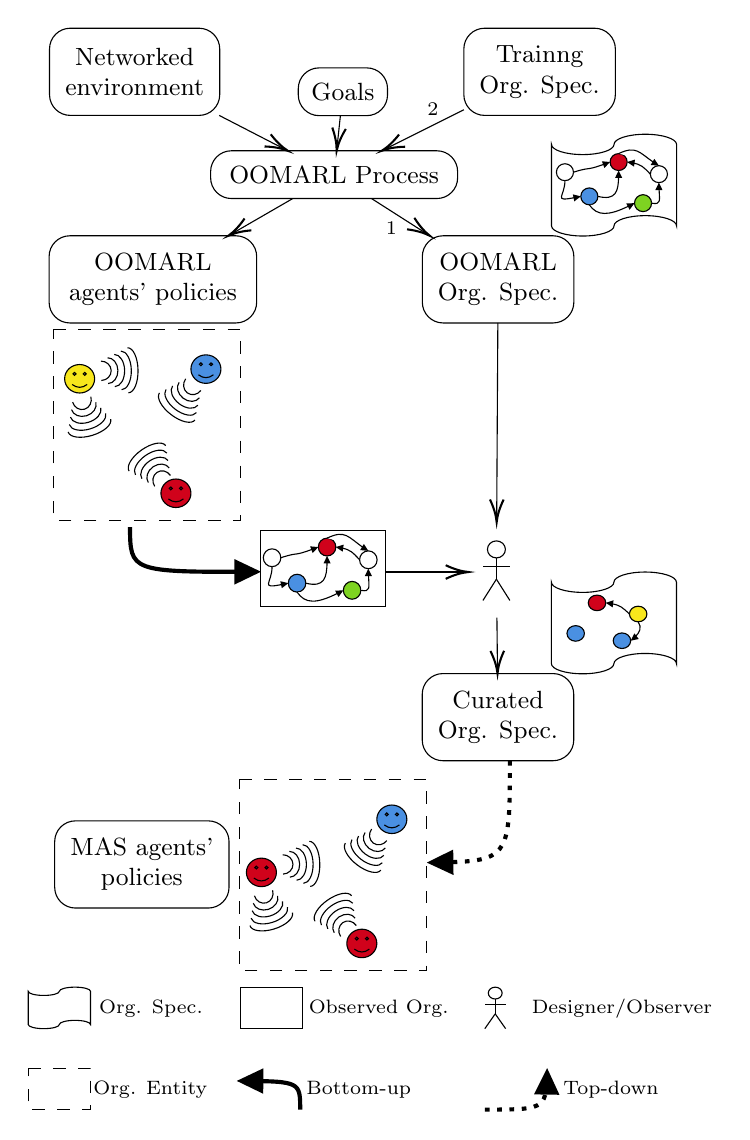
\begin{tikzpicture}[x=0.75pt,y=0.75pt,yscale=-1,xscale=1]
%uncomment if require: \path (0,567); %set diagram left start at 0, and has height of 567

%Flowchart: Punched Tape [id:dp09352793636343182] 
\draw  [fill={rgb, 255:red, 255; green, 255; blue, 255 }  ,fill opacity=1 ] (260,284.9) .. controls (260,287.61) and (266.74,289.81) .. (275.06,289.81) .. controls (283.38,289.81) and (290.12,287.61) .. (290.12,284.9) .. controls (290.12,282.2) and (296.87,280) .. (305.18,280) .. controls (313.5,280) and (320.25,282.2) .. (320.25,284.9) -- (320.25,324.13) .. controls (320.25,321.42) and (313.5,319.23) .. (305.18,319.23) .. controls (296.87,319.23) and (290.12,321.42) .. (290.12,324.13) .. controls (290.12,326.84) and (283.38,329.03) .. (275.06,329.03) .. controls (266.74,329.03) and (260,326.84) .. (260,324.13) -- cycle ;
%Shape: Ellipse [id:dp8537944349912123] 
\draw  [fill={rgb, 255:red, 208; green, 2; blue, 27 }  ,fill opacity=1 ] (277.77,294.86) .. controls (277.77,292.79) and (279.66,291.11) .. (281.98,291.11) .. controls (284.3,291.11) and (286.19,292.79) .. (286.19,294.86) .. controls (286.19,296.94) and (284.3,298.62) .. (281.98,298.62) .. controls (279.66,298.62) and (277.77,296.94) .. (277.77,294.86) -- cycle ;
%Shape: Ellipse [id:dp6897748103188357] 
\draw  [fill={rgb, 255:red, 248; green, 231; blue, 28 }  ,fill opacity=1 ] (297.6,300.23) .. controls (297.6,298.15) and (299.49,296.47) .. (301.81,296.47) .. controls (304.13,296.47) and (306.02,298.15) .. (306.02,300.23) .. controls (306.02,302.3) and (304.13,303.98) .. (301.81,303.98) .. controls (299.49,303.98) and (297.6,302.3) .. (297.6,300.23) -- cycle ;
%Shape: Ellipse [id:dp4802320082509959] 
\draw  [fill={rgb, 255:red, 74; green, 144; blue, 226 }  ,fill opacity=1 ] (289.79,313.09) .. controls (289.79,311.02) and (291.67,309.34) .. (294,309.34) .. controls (296.32,309.34) and (298.2,311.02) .. (298.2,313.09) .. controls (298.2,315.17) and (296.32,316.85) .. (294,316.85) .. controls (291.67,316.85) and (289.79,315.17) .. (289.79,313.09) -- cycle ;
%Curve Lines [id:da7546101861138359] 
\draw [fill={rgb, 255:red, 255; green, 255; blue, 255 }  ,fill opacity=1 ]   (297.6,300.23) .. controls (294.11,296.93) and (293.1,296) .. (289.08,295.29) ;
\draw [shift={(286.19,294.86)}, rotate = 7.39] [fill={rgb, 255:red, 0; green, 0; blue, 0 }  ][line width=0.08]  [draw opacity=0] (3.57,-1.72) -- (0,0) -- (3.57,1.72) -- cycle    ;
%Shape: Ellipse [id:dp693668966316707] 
\draw  [fill={rgb, 255:red, 74; green, 144; blue, 226 }  ,fill opacity=1 ] (267.5,309.58) .. controls (267.5,307.51) and (269.38,305.83) .. (271.71,305.83) .. controls (274.03,305.83) and (275.91,307.51) .. (275.91,309.58) .. controls (275.91,311.65) and (274.03,313.33) .. (271.71,313.33) .. controls (269.38,313.33) and (267.5,311.65) .. (267.5,309.58) -- cycle ;
%Curve Lines [id:da5612242217579502] 
\draw [fill={rgb, 255:red, 255; green, 255; blue, 255 }  ,fill opacity=1 ]   (301.81,303.98) .. controls (303.69,306.69) and (302.57,309.05) .. (300.45,311.16) ;
\draw [shift={(298.2,313.09)}, rotate = 322.38] [fill={rgb, 255:red, 0; green, 0; blue, 0 }  ][line width=0.08]  [draw opacity=0] (3.57,-1.72) -- (0,0) -- (3.57,1.72) -- cycle    ;

%Shape: Rectangle [id:dp7949048767988509] 
\draw  [dash pattern={on 4.5pt off 4.5pt}] (20.05,163.11) -- (110.42,163.11) -- (110.42,255.04) -- (20.05,255.04) -- cycle ;
%Shape: Smiley Face [id:dp8425156316307105] 
\draw  [fill={rgb, 255:red, 248; green, 231; blue, 28 }  ,fill opacity=1 ] (25.48,186.89) .. controls (25.48,183.1) and (28.71,180.03) .. (32.71,180.03) .. controls (36.7,180.03) and (39.94,183.1) .. (39.94,186.89) .. controls (39.94,190.68) and (36.7,193.75) .. (32.71,193.75) .. controls (28.71,193.75) and (25.48,190.68) .. (25.48,186.89) -- cycle ; \draw  [fill={rgb, 255:red, 248; green, 231; blue, 28 }  ,fill opacity=1 ] (29.53,184.56) .. controls (29.53,184.18) and (29.85,183.87) .. (30.25,183.87) .. controls (30.65,183.87) and (30.97,184.18) .. (30.97,184.56) .. controls (30.97,184.94) and (30.65,185.24) .. (30.25,185.24) .. controls (29.85,185.24) and (29.53,184.94) .. (29.53,184.56) -- cycle ; \draw  [fill={rgb, 255:red, 248; green, 231; blue, 28 }  ,fill opacity=1 ] (34.44,184.56) .. controls (34.44,184.18) and (34.77,183.87) .. (35.16,183.87) .. controls (35.56,183.87) and (35.89,184.18) .. (35.89,184.56) .. controls (35.89,184.94) and (35.56,185.24) .. (35.16,185.24) .. controls (34.77,185.24) and (34.44,184.94) .. (34.44,184.56) -- cycle ; \draw   (29.09,189.64) .. controls (31.5,191.47) and (33.91,191.47) .. (36.32,189.64) ;
%Shape: Arc [id:dp7103754459108031] 
\draw  [draw opacity=0] (47.66,206.32) .. controls (47.66,206.32) and (47.66,206.32) .. (47.66,206.32) .. controls (48.43,208.93) and (44.47,212.43) .. (38.81,214.15) .. controls (33.16,215.87) and (27.96,215.15) .. (27.19,212.54) -- (37.43,209.43) -- cycle ; \draw   (47.66,206.32) .. controls (47.66,206.32) and (47.66,206.32) .. (47.66,206.32) .. controls (48.43,208.93) and (44.47,212.43) .. (38.81,214.15) .. controls (33.16,215.87) and (27.96,215.15) .. (27.19,212.54) ;  
%Shape: Arc [id:dp9993647702991559] 
\draw  [draw opacity=0] (45.27,203.61) .. controls (46.04,206.22) and (42.73,209.53) .. (37.89,211) .. controls (33.04,212.48) and (28.49,211.55) .. (27.73,208.94) -- (36.5,206.28) -- cycle ; \draw   (45.27,203.61) .. controls (46.04,206.22) and (42.73,209.53) .. (37.89,211) .. controls (33.04,212.48) and (28.49,211.55) .. (27.73,208.94) ;  
%Shape: Arc [id:dp33021260729129986] 
\draw  [draw opacity=0] (42.88,200.9) .. controls (42.88,200.9) and (42.88,200.9) .. (42.88,200.9) .. controls (43.65,203.51) and (41,206.62) .. (36.96,207.85) .. controls (32.92,209.08) and (29.03,207.96) .. (28.26,205.35) -- (35.57,203.12) -- cycle ; \draw   (42.88,200.9) .. controls (42.88,200.9) and (42.88,200.9) .. (42.88,200.9) .. controls (43.65,203.51) and (41,206.62) .. (36.96,207.85) .. controls (32.92,209.08) and (29.03,207.96) .. (28.26,205.35) ;  
%Shape: Arc [id:dp7515950702187679] 
\draw  [draw opacity=0] (40.5,198.2) .. controls (40.5,198.2) and (40.5,198.2) .. (40.5,198.2) .. controls (40.5,198.2) and (40.5,198.2) .. (40.5,198.2) .. controls (41.26,200.81) and (39.27,203.72) .. (36.04,204.7) .. controls (32.81,205.68) and (29.57,204.36) .. (28.8,201.75) .. controls (28.8,201.75) and (28.8,201.75) .. (28.8,201.75) -- (34.65,199.97) -- cycle ; \draw   (40.5,198.2) .. controls (40.5,198.2) and (40.5,198.2) .. (40.5,198.2) .. controls (40.5,198.2) and (40.5,198.2) .. (40.5,198.2) .. controls (41.26,200.81) and (39.27,203.72) .. (36.04,204.7) .. controls (32.81,205.68) and (29.57,204.36) .. (28.8,201.75) .. controls (28.8,201.75) and (28.8,201.75) .. (28.8,201.75) ;  
%Shape: Arc [id:dp17995425823285305] 
\draw  [draw opacity=0] (38.11,195.49) .. controls (38.11,195.49) and (38.11,195.49) .. (38.11,195.49) .. controls (38.11,195.49) and (38.11,195.49) .. (38.11,195.49) .. controls (38.88,198.1) and (37.53,200.81) .. (35.11,201.55) .. controls (32.69,202.29) and (30.1,200.77) .. (29.34,198.16) -- (33.72,196.82) -- cycle ; \draw   (38.11,195.49) .. controls (38.11,195.49) and (38.11,195.49) .. (38.11,195.49) .. controls (38.11,195.49) and (38.11,195.49) .. (38.11,195.49) .. controls (38.88,198.1) and (37.53,200.81) .. (35.11,201.55) .. controls (32.69,202.29) and (30.1,200.77) .. (29.34,198.16) ;  

%Shape: Arc [id:dp8934563741256025] 
\draw  [draw opacity=0] (55.78,171.93) .. controls (58.46,171.87) and (60.73,176.69) .. (60.84,182.69) .. controls (60.96,188.7) and (58.88,193.6) .. (56.21,193.66) -- (55.99,182.79) -- cycle ; \draw   (55.78,171.93) .. controls (58.46,171.87) and (60.73,176.69) .. (60.84,182.69) .. controls (60.96,188.7) and (58.88,193.6) .. (56.21,193.66) ;  
%Shape: Arc [id:dp5963815446588989] 
\draw  [draw opacity=0] (52.58,173.54) .. controls (55.26,173.49) and (57.51,177.62) .. (57.61,182.76) .. controls (57.71,187.9) and (55.62,192.12) .. (52.94,192.17) -- (52.76,182.86) -- cycle ; \draw   (52.58,173.54) .. controls (55.26,173.49) and (57.51,177.62) .. (57.61,182.76) .. controls (57.71,187.9) and (55.62,192.12) .. (52.94,192.17) ;  
%Shape: Arc [id:dp3378668028957823] 
\draw  [draw opacity=0] (49.38,175.16) .. controls (49.38,175.16) and (49.38,175.16) .. (49.38,175.16) .. controls (49.38,175.16) and (49.38,175.16) .. (49.38,175.16) .. controls (52.06,175.11) and (54.3,178.54) .. (54.38,182.82) .. controls (54.46,187.11) and (52.36,190.63) .. (49.68,190.68) -- (49.53,182.92) -- cycle ; \draw   (49.38,175.16) .. controls (49.38,175.16) and (49.38,175.16) .. (49.38,175.16) .. controls (49.38,175.16) and (49.38,175.16) .. (49.38,175.16) .. controls (52.06,175.11) and (54.3,178.54) .. (54.38,182.82) .. controls (54.46,187.11) and (52.36,190.63) .. (49.68,190.68) ;  
%Shape: Arc [id:dp7870035207223711] 
\draw  [draw opacity=0] (46.18,176.78) .. controls (48.86,176.72) and (51.08,179.46) .. (51.15,182.89) .. controls (51.21,186.32) and (49.1,189.14) .. (46.42,189.2) -- (46.3,182.99) -- cycle ; \draw   (46.18,176.78) .. controls (48.86,176.72) and (51.08,179.46) .. (51.15,182.89) .. controls (51.21,186.32) and (49.1,189.14) .. (46.42,189.2) ;  
%Shape: Arc [id:dp7731275981870975] 
\draw  [draw opacity=0] (42.98,178.39) .. controls (42.98,178.39) and (42.98,178.39) .. (42.98,178.39) .. controls (45.65,178.34) and (47.86,180.38) .. (47.91,182.95) .. controls (47.96,185.53) and (45.83,187.65) .. (43.16,187.71) -- (43.07,183.05) -- cycle ; \draw   (42.98,178.39) .. controls (42.98,178.39) and (42.98,178.39) .. (42.98,178.39) .. controls (45.65,178.34) and (47.86,180.38) .. (47.91,182.95) .. controls (47.96,185.53) and (45.83,187.65) .. (43.16,187.71) ;  

%Shape: Smiley Face [id:dp9460068866596214] 
\draw  [fill={rgb, 255:red, 208; green, 2; blue, 27 }  ,fill opacity=1 ] (71.87,242.05) .. controls (71.87,238.26) and (75.1,235.19) .. (79.1,235.19) .. controls (83.09,235.19) and (86.33,238.26) .. (86.33,242.05) .. controls (86.33,245.84) and (83.09,248.92) .. (79.1,248.92) .. controls (75.1,248.92) and (71.87,245.84) .. (71.87,242.05) -- cycle ; \draw  [fill={rgb, 255:red, 208; green, 2; blue, 27 }  ,fill opacity=1 ] (75.91,239.72) .. controls (75.91,239.34) and (76.24,239.03) .. (76.64,239.03) .. controls (77.04,239.03) and (77.36,239.34) .. (77.36,239.72) .. controls (77.36,240.1) and (77.04,240.4) .. (76.64,240.4) .. controls (76.24,240.4) and (75.91,240.1) .. (75.91,239.72) -- cycle ; \draw  [fill={rgb, 255:red, 208; green, 2; blue, 27 }  ,fill opacity=1 ] (80.83,239.72) .. controls (80.83,239.34) and (81.15,239.03) .. (81.55,239.03) .. controls (81.95,239.03) and (82.28,239.34) .. (82.28,239.72) .. controls (82.28,240.1) and (81.95,240.4) .. (81.55,240.4) .. controls (81.15,240.4) and (80.83,240.1) .. (80.83,239.72) -- cycle ; \draw   (75.48,244.8) .. controls (77.89,246.63) and (80.3,246.63) .. (82.71,244.8) ;
%Shape: Arc [id:dp2662505393390908] 
\draw  [draw opacity=0] (56.53,231.38) .. controls (56.53,231.38) and (56.53,231.38) .. (56.53,231.38) .. controls (56.53,231.38) and (56.53,231.38) .. (56.53,231.38) .. controls (55.02,229.13) and (57.74,224.56) .. (62.6,221.17) .. controls (67.47,217.77) and (72.64,216.84) .. (74.15,219.09) -- (65.34,225.24) -- cycle ; \draw   (56.53,231.38) .. controls (56.53,231.38) and (56.53,231.38) .. (56.53,231.38) .. controls (56.53,231.38) and (56.53,231.38) .. (56.53,231.38) .. controls (55.02,229.13) and (57.74,224.56) .. (62.6,221.17) .. controls (67.47,217.77) and (72.64,216.84) .. (74.15,219.09) ;  
%Shape: Arc [id:dp5533657200850002] 
\draw  [draw opacity=0] (59.62,233.22) .. controls (59.62,233.22) and (59.62,233.22) .. (59.62,233.22) .. controls (58.11,230.97) and (60.26,226.79) .. (64.43,223.88) .. controls (68.6,220.97) and (73.21,220.43) .. (74.72,222.68) -- (67.17,227.95) -- cycle ; \draw   (59.62,233.22) .. controls (59.62,233.22) and (59.62,233.22) .. (59.62,233.22) .. controls (58.11,230.97) and (60.26,226.79) .. (64.43,223.88) .. controls (68.6,220.97) and (73.21,220.43) .. (74.72,222.68) ;  
%Shape: Arc [id:dp130720604660594] 
\draw  [draw opacity=0] (62.71,235.05) .. controls (61.19,232.8) and (62.78,229.02) .. (66.26,226.59) .. controls (69.73,224.17) and (73.78,224.02) .. (75.29,226.27) -- (69,230.66) -- cycle ; \draw   (62.71,235.05) .. controls (61.19,232.8) and (62.78,229.02) .. (66.26,226.59) .. controls (69.73,224.17) and (73.78,224.02) .. (75.29,226.27) ;  
%Shape: Arc [id:dp7777326608896638] 
\draw  [draw opacity=0] (65.79,236.88) .. controls (65.79,236.88) and (65.79,236.88) .. (65.79,236.88) .. controls (64.28,234.64) and (65.31,231.24) .. (68.09,229.3) .. controls (70.87,227.36) and (74.35,227.61) .. (75.86,229.86) -- (70.83,233.37) -- cycle ; \draw   (65.79,236.88) .. controls (65.79,236.88) and (65.79,236.88) .. (65.79,236.88) .. controls (64.28,234.64) and (65.31,231.24) .. (68.09,229.3) .. controls (70.87,227.36) and (74.35,227.61) .. (75.86,229.86) ;  
%Shape: Arc [id:dp4348101062357661] 
\draw  [draw opacity=0] (68.88,238.72) .. controls (67.37,236.47) and (67.83,233.47) .. (69.92,232.02) .. controls (72,230.56) and (74.92,231.2) .. (76.43,233.45) -- (72.66,236.08) -- cycle ; \draw   (68.88,238.72) .. controls (67.37,236.47) and (67.83,233.47) .. (69.92,232.02) .. controls (72,230.56) and (74.92,231.2) .. (76.43,233.45) ;  

%Shape: Smiley Face [id:dp40321958667865143] 
\draw  [fill={rgb, 255:red, 74; green, 144; blue, 226 }  ,fill opacity=1 ] (86.33,182.23) .. controls (86.33,178.44) and (89.56,175.37) .. (93.55,175.37) .. controls (97.55,175.37) and (100.78,178.44) .. (100.78,182.23) .. controls (100.78,186.02) and (97.55,189.1) .. (93.55,189.1) .. controls (89.56,189.1) and (86.33,186.02) .. (86.33,182.23) -- cycle ; \draw  [fill={rgb, 255:red, 74; green, 144; blue, 226 }  ,fill opacity=1 ] (90.37,179.9) .. controls (90.37,179.52) and (90.7,179.21) .. (91.1,179.21) .. controls (91.5,179.21) and (91.82,179.52) .. (91.82,179.9) .. controls (91.82,180.28) and (91.5,180.58) .. (91.1,180.58) .. controls (90.7,180.58) and (90.37,180.28) .. (90.37,179.9) -- cycle ; \draw  [fill={rgb, 255:red, 74; green, 144; blue, 226 }  ,fill opacity=1 ] (95.29,179.9) .. controls (95.29,179.52) and (95.61,179.21) .. (96.01,179.21) .. controls (96.41,179.21) and (96.74,179.52) .. (96.74,179.9) .. controls (96.74,180.28) and (96.41,180.58) .. (96.01,180.58) .. controls (95.61,180.58) and (95.29,180.28) .. (95.29,179.9) -- cycle ; \draw   (89.94,184.98) .. controls (92.35,186.81) and (94.76,186.81) .. (97.17,184.98) ;
%Shape: Arc [id:dp6344973920370733] 
\draw  [draw opacity=0] (88.26,206.75) .. controls (88.26,206.75) and (88.26,206.75) .. (88.26,206.75) .. controls (86.65,208.93) and (81.52,207.78) .. (76.8,204.18) .. controls (72.08,200.58) and (69.55,195.9) .. (71.16,193.72) -- (79.71,200.23) -- cycle ; \draw   (88.26,206.75) .. controls (88.26,206.75) and (88.26,206.75) .. (88.26,206.75) .. controls (86.65,208.93) and (81.52,207.78) .. (76.8,204.18) .. controls (72.08,200.58) and (69.55,195.9) .. (71.16,193.72) ;  
%Shape: Arc [id:dp2502725185770005] 
\draw  [draw opacity=0] (88.97,203.19) .. controls (88.97,203.19) and (88.97,203.19) .. (88.97,203.19) .. controls (88.97,203.19) and (88.97,203.19) .. (88.97,203.19) .. controls (87.37,205.37) and (82.78,204.63) .. (78.74,201.55) .. controls (74.69,198.46) and (72.71,194.2) .. (74.32,192.02) -- (81.65,197.6) -- cycle ; \draw   (88.97,203.19) .. controls (88.97,203.19) and (88.97,203.19) .. (88.97,203.19) .. controls (88.97,203.19) and (88.97,203.19) .. (88.97,203.19) .. controls (87.37,205.37) and (82.78,204.63) .. (78.74,201.55) .. controls (74.69,198.46) and (72.71,194.2) .. (74.32,192.02) ;  
%Shape: Arc [id:dp23421846029392612] 
\draw  [draw opacity=0] (89.69,199.63) .. controls (89.69,199.63) and (89.69,199.63) .. (89.69,199.63) .. controls (89.69,199.63) and (89.69,199.63) .. (89.69,199.63) .. controls (88.08,201.81) and (84.05,201.49) .. (80.68,198.92) .. controls (77.3,196.35) and (75.87,192.5) .. (77.48,190.32) -- (83.58,194.97) -- cycle ; \draw   (89.69,199.63) .. controls (89.69,199.63) and (89.69,199.63) .. (89.69,199.63) .. controls (89.69,199.63) and (89.69,199.63) .. (89.69,199.63) .. controls (88.08,201.81) and (84.05,201.49) .. (80.68,198.92) .. controls (77.3,196.35) and (75.87,192.5) .. (77.48,190.32) ;  
%Shape: Arc [id:dp02946644855410807] 
\draw  [draw opacity=0] (90.41,196.06) .. controls (88.8,198.24) and (85.31,198.34) .. (82.62,196.29) .. controls (79.92,194.23) and (79.03,190.8) .. (80.64,188.62) -- (85.52,192.34) -- cycle ; \draw   (90.41,196.06) .. controls (88.8,198.24) and (85.31,198.34) .. (82.62,196.29) .. controls (79.92,194.23) and (79.03,190.8) .. (80.64,188.62) ;  
%Shape: Arc [id:dp07919277634076938] 
\draw  [draw opacity=0] (91.13,192.5) .. controls (91.13,192.5) and (91.13,192.5) .. (91.13,192.5) .. controls (89.52,194.68) and (86.58,195.2) .. (84.55,193.66) .. controls (82.53,192.11) and (82.19,189.1) .. (83.8,186.92) -- (87.46,189.71) -- cycle ; \draw   (91.13,192.5) .. controls (91.13,192.5) and (91.13,192.5) .. (91.13,192.5) .. controls (89.52,194.68) and (86.58,195.2) .. (84.55,193.66) .. controls (82.53,192.11) and (82.19,189.1) .. (83.8,186.92) ;  

%Shape: Ellipse [id:dp5665300419613197] 
\draw   (229.18,269.1) .. controls (229.18,266.84) and (231.12,265) .. (233.51,265) .. controls (235.9,265) and (237.84,266.84) .. (237.84,269.1) .. controls (237.84,271.36) and (235.9,273.2) .. (233.51,273.2) .. controls (231.12,273.2) and (229.18,271.36) .. (229.18,269.1) -- cycle ;
%Straight Lines [id:da868287133321088] 
\draw    (233.51,273.2) -- (233.51,283.45) ;
%Straight Lines [id:da7338999456859931] 
\draw    (233.51,283.45) -- (227.02,293.7) ;
%Straight Lines [id:da7618645013452761] 
\draw    (233.51,283.45) -- (240,293.7) ;
%Straight Lines [id:da7029210082761028] 
\draw    (240,277.3) -- (227.02,277.3) ;

%Shape: Rectangle [id:dp36259598060414655] 
\draw  [fill={rgb, 255:red, 255; green, 255; blue, 255 }  ,fill opacity=1 ] (120,260) -- (180.25,260) -- (180.25,296.77) -- (120,296.77) -- cycle ;
%Shape: Ellipse [id:dp34598635042601256] 
\draw  [fill={rgb, 255:red, 255; green, 255; blue, 255 }  ,fill opacity=1 ] (121.2,273.12) .. controls (121.2,270.75) and (123.09,268.83) .. (125.42,268.83) .. controls (127.75,268.83) and (129.64,270.75) .. (129.64,273.12) .. controls (129.64,275.49) and (127.75,277.41) .. (125.42,277.41) .. controls (123.09,277.41) and (121.2,275.49) .. (121.2,273.12) -- cycle ;
%Shape: Ellipse [id:dp0011247415244253212] 
\draw  [fill={rgb, 255:red, 74; green, 144; blue, 226 }  ,fill opacity=1 ] (133.25,285.37) .. controls (133.25,283) and (135.14,281.08) .. (137.47,281.08) .. controls (139.8,281.08) and (141.69,283) .. (141.69,285.37) .. controls (141.69,287.74) and (139.8,289.66) .. (137.47,289.66) .. controls (135.14,289.66) and (133.25,287.74) .. (133.25,285.37) -- cycle ;
%Shape: Ellipse [id:dp8822927144483022] 
\draw  [fill={rgb, 255:red, 208; green, 2; blue, 27 }  ,fill opacity=1 ] (147.71,267.97) .. controls (147.71,265.6) and (149.6,263.68) .. (151.93,263.68) .. controls (154.26,263.68) and (156.15,265.6) .. (156.15,267.97) .. controls (156.15,270.34) and (154.26,272.26) .. (151.93,272.26) .. controls (149.6,272.26) and (147.71,270.34) .. (147.71,267.97) -- cycle ;
%Shape: Ellipse [id:dp7611446545020739] 
\draw  [fill={rgb, 255:red, 255; green, 255; blue, 255 }  ,fill opacity=1 ] (167.59,274.1) .. controls (167.59,271.73) and (169.48,269.81) .. (171.81,269.81) .. controls (174.14,269.81) and (176.03,271.73) .. (176.03,274.1) .. controls (176.03,276.47) and (174.14,278.39) .. (171.81,278.39) .. controls (169.48,278.39) and (167.59,276.47) .. (167.59,274.1) -- cycle ;
%Shape: Ellipse [id:dp1592826898001829] 
\draw  [fill={rgb, 255:red, 126; green, 211; blue, 33 }  ,fill opacity=1 ] (159.76,288.81) .. controls (159.76,286.44) and (161.65,284.52) .. (163.98,284.52) .. controls (166.31,284.52) and (168.2,286.44) .. (168.2,288.81) .. controls (168.2,291.18) and (166.31,293.1) .. (163.98,293.1) .. controls (161.65,293.1) and (159.76,291.18) .. (159.76,288.81) -- cycle ;
%Curve Lines [id:da27399536046205264] 
\draw [fill={rgb, 255:red, 255; green, 255; blue, 255 }  ,fill opacity=1 ]   (129.64,273.12) .. controls (139.11,270.05) and (134.67,272.76) .. (144.92,269.01) ;
\draw [shift={(147.71,267.97)}, rotate = 159.17] [fill={rgb, 255:red, 0; green, 0; blue, 0 }  ][line width=0.08]  [draw opacity=0] (3.57,-1.72) -- (0,0) -- (3.57,1.72) -- cycle    ;
%Curve Lines [id:da16623917428090795] 
\draw [fill={rgb, 255:red, 255; green, 255; blue, 255 }  ,fill opacity=1 ]   (141.69,285.37) .. controls (150.75,287.65) and (151.79,282.63) .. (151.91,275.25) ;
\draw [shift={(151.93,272.26)}, rotate = 90] [fill={rgb, 255:red, 0; green, 0; blue, 0 }  ][line width=0.08]  [draw opacity=0] (3.57,-1.72) -- (0,0) -- (3.57,1.72) -- cycle    ;
%Curve Lines [id:da46234775845087284] 
\draw [fill={rgb, 255:red, 255; green, 255; blue, 255 }  ,fill opacity=1 ]   (167.59,274.1) .. controls (164.09,270.33) and (163.08,269.27) .. (159.05,268.46) ;
\draw [shift={(156.15,267.97)}, rotate = 8.42] [fill={rgb, 255:red, 0; green, 0; blue, 0 }  ][line width=0.08]  [draw opacity=0] (3.57,-1.72) -- (0,0) -- (3.57,1.72) -- cycle    ;
%Curve Lines [id:da3119386523209393] 
\draw [fill={rgb, 255:red, 255; green, 255; blue, 255 }  ,fill opacity=1 ]   (168.2,288.81) .. controls (172.97,289.67) and (172.14,287.87) .. (171.87,281.33) ;
\draw [shift={(171.81,278.39)}, rotate = 90] [fill={rgb, 255:red, 0; green, 0; blue, 0 }  ][line width=0.08]  [draw opacity=0] (3.57,-1.72) -- (0,0) -- (3.57,1.72) -- cycle    ;
%Curve Lines [id:da8983756138417751] 
\draw [fill={rgb, 255:red, 255; green, 255; blue, 255 }  ,fill opacity=1 ]   (125.42,277.41) .. controls (125.42,285.5) and (119.17,288.19) .. (130.41,285.96) ;
\draw [shift={(133.25,285.37)}, rotate = 168.05] [fill={rgb, 255:red, 0; green, 0; blue, 0 }  ][line width=0.08]  [draw opacity=0] (3.57,-1.72) -- (0,0) -- (3.57,1.72) -- cycle    ;
%Curve Lines [id:da8579733900345894] 
\draw [fill={rgb, 255:red, 255; green, 255; blue, 255 }  ,fill opacity=1 ]   (137.47,289.66) .. controls (141.37,295.45) and (146.82,295.36) .. (157.15,290.17) ;
\draw [shift={(159.76,288.81)}, rotate = 151.67] [fill={rgb, 255:red, 0; green, 0; blue, 0 }  ][line width=0.08]  [draw opacity=0] (3.57,-1.72) -- (0,0) -- (3.57,1.72) -- cycle    ;
%Curve Lines [id:da598997074659714] 
\draw [fill={rgb, 255:red, 255; green, 255; blue, 255 }  ,fill opacity=1 ]   (151.93,263.68) .. controls (160.7,259.44) and (161.99,263.12) .. (169.42,268.25) ;
\draw [shift={(171.81,269.81)}, rotate = 211.4] [fill={rgb, 255:red, 0; green, 0; blue, 0 }  ][line width=0.08]  [draw opacity=0] (3.57,-1.72) -- (0,0) -- (3.57,1.72) -- cycle    ;

%Shape: Boxed Bezier Curve [id:dp04329100663395624] 
\draw [line width=1.5]    (56.97,258.4) .. controls (57.12,279.64) and (57.12,280.06) .. (116.36,279.88) ;
\draw [shift={(120.07,279.86)}, rotate = 179.81] [fill={rgb, 255:red, 0; green, 0; blue, 0 }  ][line width=0.08]  [draw opacity=0] (12.77,-6.13) -- (0,0) -- (12.77,6.13) -- cycle    ;
%Shape: Boxed Bezier Curve [id:dp3249540323733473] 
\draw [line width=1.5]  [dash pattern={on 1.69pt off 2.76pt}]  (240,371) .. controls (240,377.31) and (240,382.8) .. (239.91,387.58) .. controls (239.34,418.4) and (235.11,419.53) .. (203.54,419.96) ;
\draw [shift={(200,420)}, rotate = 359.3] [fill={rgb, 255:red, 0; green, 0; blue, 0 }  ][line width=0.08]  [draw opacity=0] (12.77,-6.13) -- (0,0) -- (12.77,6.13) -- cycle    ;
%Shape: Rectangle [id:dp3591393250200341] 
\draw  [dash pattern={on 4.5pt off 4.5pt}] (109.63,380) -- (200,380) -- (200,471.94) -- (109.63,471.94) -- cycle ;
%Shape: Smiley Face [id:dp3801591887945033] 
\draw  [fill={rgb, 255:red, 208; green, 2; blue, 27 }  ,fill opacity=1 ] (113.05,424.72) .. controls (113.05,420.92) and (116.29,417.85) .. (120.28,417.85) .. controls (124.28,417.85) and (127.51,420.92) .. (127.51,424.72) .. controls (127.51,428.51) and (124.28,431.58) .. (120.28,431.58) .. controls (116.29,431.58) and (113.05,428.51) .. (113.05,424.72) -- cycle ; \draw  [fill={rgb, 255:red, 208; green, 2; blue, 27 }  ,fill opacity=1 ] (117.1,422.38) .. controls (117.1,422) and (117.43,421.7) .. (117.82,421.7) .. controls (118.22,421.7) and (118.55,422) .. (118.55,422.38) .. controls (118.55,422.76) and (118.22,423.07) .. (117.82,423.07) .. controls (117.43,423.07) and (117.1,422.76) .. (117.1,422.38) -- cycle ; \draw  [fill={rgb, 255:red, 208; green, 2; blue, 27 }  ,fill opacity=1 ] (122.02,422.38) .. controls (122.02,422) and (122.34,421.7) .. (122.74,421.7) .. controls (123.14,421.7) and (123.46,422) .. (123.46,422.38) .. controls (123.46,422.76) and (123.14,423.07) .. (122.74,423.07) .. controls (122.34,423.07) and (122.02,422.76) .. (122.02,422.38) -- cycle ; \draw   (116.67,427.46) .. controls (119.08,429.29) and (121.49,429.29) .. (123.9,427.46) ;
%Shape: Arc [id:dp40222913228483237] 
\draw  [draw opacity=0] (135.24,444.14) .. controls (135.24,444.14) and (135.24,444.14) .. (135.24,444.14) .. controls (136,446.75) and (132.04,450.26) .. (126.39,451.98) .. controls (120.74,453.7) and (115.53,452.97) .. (114.77,450.36) -- (125,447.25) -- cycle ; \draw   (135.24,444.14) .. controls (135.24,444.14) and (135.24,444.14) .. (135.24,444.14) .. controls (136,446.75) and (132.04,450.26) .. (126.39,451.98) .. controls (120.74,453.7) and (115.53,452.97) .. (114.77,450.36) ;  
%Shape: Arc [id:dp6185790641450695] 
\draw  [draw opacity=0] (132.85,441.43) .. controls (133.62,444.05) and (130.31,447.36) .. (125.46,448.83) .. controls (120.62,450.3) and (116.07,449.38) .. (115.3,446.77) -- (124.08,444.1) -- cycle ; \draw   (132.85,441.43) .. controls (133.62,444.05) and (130.31,447.36) .. (125.46,448.83) .. controls (120.62,450.3) and (116.07,449.38) .. (115.3,446.77) ;  
%Shape: Arc [id:dp6749114191148724] 
\draw  [draw opacity=0] (130.46,438.73) .. controls (130.46,438.73) and (130.46,438.73) .. (130.46,438.73) .. controls (131.23,441.34) and (128.58,444.45) .. (124.54,445.68) .. controls (120.5,446.9) and (116.61,445.78) .. (115.84,443.17) -- (123.15,440.95) -- cycle ; \draw   (130.46,438.73) .. controls (130.46,438.73) and (130.46,438.73) .. (130.46,438.73) .. controls (131.23,441.34) and (128.58,444.45) .. (124.54,445.68) .. controls (120.5,446.9) and (116.61,445.78) .. (115.84,443.17) ;  
%Shape: Arc [id:dp056403546095020296] 
\draw  [draw opacity=0] (128.07,436.02) .. controls (128.07,436.02) and (128.07,436.02) .. (128.07,436.02) .. controls (128.07,436.02) and (128.07,436.02) .. (128.07,436.02) .. controls (128.84,438.63) and (126.84,441.54) .. (123.61,442.53) .. controls (120.38,443.51) and (117.14,442.19) .. (116.38,439.58) -- (122.22,437.8) -- cycle ; \draw   (128.07,436.02) .. controls (128.07,436.02) and (128.07,436.02) .. (128.07,436.02) .. controls (128.07,436.02) and (128.07,436.02) .. (128.07,436.02) .. controls (128.84,438.63) and (126.84,441.54) .. (123.61,442.53) .. controls (120.38,443.51) and (117.14,442.19) .. (116.38,439.58) ;  
%Shape: Arc [id:dp048963270262922354] 
\draw  [draw opacity=0] (125.69,433.32) .. controls (125.69,433.32) and (125.69,433.32) .. (125.69,433.32) .. controls (126.45,435.93) and (125.11,438.64) .. (122.69,439.38) .. controls (120.27,440.11) and (117.68,438.59) .. (116.91,435.98) -- (121.3,434.65) -- cycle ; \draw   (125.69,433.32) .. controls (125.69,433.32) and (125.69,433.32) .. (125.69,433.32) .. controls (126.45,435.93) and (125.11,438.64) .. (122.69,439.38) .. controls (120.27,440.11) and (117.68,438.59) .. (116.91,435.98) ;  

%Shape: Arc [id:dp11791815378481285] 
\draw  [draw opacity=0] (143.36,409.75) .. controls (143.36,409.75) and (143.36,409.75) .. (143.36,409.75) .. controls (146.04,409.7) and (148.3,414.52) .. (148.42,420.52) .. controls (148.54,426.52) and (146.46,431.43) .. (143.78,431.48) -- (143.57,420.62) -- cycle ; \draw   (143.36,409.75) .. controls (143.36,409.75) and (143.36,409.75) .. (143.36,409.75) .. controls (146.04,409.7) and (148.3,414.52) .. (148.42,420.52) .. controls (148.54,426.52) and (146.46,431.43) .. (143.78,431.48) ;  
%Shape: Arc [id:dp6186444432706435] 
\draw  [draw opacity=0] (140.16,411.37) .. controls (142.84,411.32) and (145.09,415.44) .. (145.19,420.59) .. controls (145.29,425.73) and (143.2,429.94) .. (140.52,430) -- (140.34,420.68) -- cycle ; \draw   (140.16,411.37) .. controls (142.84,411.32) and (145.09,415.44) .. (145.19,420.59) .. controls (145.29,425.73) and (143.2,429.94) .. (140.52,430) ;  
%Shape: Arc [id:dp3524256769019909] 
\draw  [draw opacity=0] (136.96,412.99) .. controls (136.96,412.99) and (136.96,412.99) .. (136.96,412.99) .. controls (139.63,412.93) and (141.87,416.36) .. (141.96,420.65) .. controls (142.04,424.94) and (139.94,428.45) .. (137.26,428.51) .. controls (137.26,428.51) and (137.26,428.51) .. (137.26,428.51) -- (137.11,420.75) -- cycle ; \draw   (136.96,412.99) .. controls (136.96,412.99) and (136.96,412.99) .. (136.96,412.99) .. controls (139.63,412.93) and (141.87,416.36) .. (141.96,420.65) .. controls (142.04,424.94) and (139.94,428.45) .. (137.26,428.51) .. controls (137.26,428.51) and (137.26,428.51) .. (137.26,428.51) ;  
%Shape: Arc [id:dp9364872182962407] 
\draw  [draw opacity=0] (133.76,414.6) .. controls (136.43,414.55) and (138.66,417.29) .. (138.72,420.72) .. controls (138.79,424.14) and (136.67,426.97) .. (134,427.02) -- (133.88,420.81) -- cycle ; \draw   (133.76,414.6) .. controls (136.43,414.55) and (138.66,417.29) .. (138.72,420.72) .. controls (138.79,424.14) and (136.67,426.97) .. (134,427.02) ;  
%Shape: Arc [id:dp43568764349824574] 
\draw  [draw opacity=0] (130.55,416.22) .. controls (130.55,416.22) and (130.55,416.22) .. (130.55,416.22) .. controls (133.23,416.17) and (135.44,418.21) .. (135.49,420.78) .. controls (135.54,423.35) and (133.41,425.48) .. (130.73,425.53) .. controls (130.73,425.53) and (130.73,425.53) .. (130.73,425.53) -- (130.64,420.88) -- cycle ; \draw   (130.55,416.22) .. controls (130.55,416.22) and (130.55,416.22) .. (130.55,416.22) .. controls (133.23,416.17) and (135.44,418.21) .. (135.49,420.78) .. controls (135.54,423.35) and (133.41,425.48) .. (130.73,425.53) .. controls (130.73,425.53) and (130.73,425.53) .. (130.73,425.53) ;  

%Shape: Smiley Face [id:dp7641236455099758] 
\draw  [fill={rgb, 255:red, 208; green, 2; blue, 27 }  ,fill opacity=1 ] (161.44,458.94) .. controls (161.44,455.15) and (164.68,452.08) .. (168.67,452.08) .. controls (172.66,452.08) and (175.9,455.15) .. (175.9,458.94) .. controls (175.9,462.73) and (172.66,465.81) .. (168.67,465.81) .. controls (164.68,465.81) and (161.44,462.73) .. (161.44,458.94) -- cycle ; \draw  [fill={rgb, 255:red, 208; green, 2; blue, 27 }  ,fill opacity=1 ] (165.49,456.61) .. controls (165.49,456.23) and (165.81,455.92) .. (166.21,455.92) .. controls (166.61,455.92) and (166.94,456.23) .. (166.94,456.61) .. controls (166.94,456.99) and (166.61,457.29) .. (166.21,457.29) .. controls (165.81,457.29) and (165.49,456.99) .. (165.49,456.61) -- cycle ; \draw  [fill={rgb, 255:red, 208; green, 2; blue, 27 }  ,fill opacity=1 ] (170.41,456.61) .. controls (170.41,456.23) and (170.73,455.92) .. (171.13,455.92) .. controls (171.53,455.92) and (171.85,456.23) .. (171.85,456.61) .. controls (171.85,456.99) and (171.53,457.29) .. (171.13,457.29) .. controls (170.73,457.29) and (170.41,456.99) .. (170.41,456.61) -- cycle ; \draw   (165.06,461.69) .. controls (167.47,463.52) and (169.88,463.52) .. (172.29,461.69) ;
%Shape: Arc [id:dp12338485660705834] 
\draw  [draw opacity=0] (146.11,448.27) .. controls (146.11,448.27) and (146.11,448.27) .. (146.11,448.27) .. controls (144.6,446.02) and (147.31,441.45) .. (152.18,438.06) .. controls (157.04,434.66) and (162.22,433.73) .. (163.73,435.98) -- (154.92,442.13) -- cycle ; \draw   (146.11,448.27) .. controls (146.11,448.27) and (146.11,448.27) .. (146.11,448.27) .. controls (144.6,446.02) and (147.31,441.45) .. (152.18,438.06) .. controls (157.04,434.66) and (162.22,433.73) .. (163.73,435.98) ;  
%Shape: Arc [id:dp047340824310728946] 
\draw  [draw opacity=0] (149.2,450.11) .. controls (149.2,450.11) and (149.2,450.11) .. (149.2,450.11) .. controls (147.68,447.86) and (149.84,443.68) .. (154.01,440.77) .. controls (158.18,437.86) and (162.79,437.32) .. (164.3,439.57) -- (156.75,444.84) -- cycle ; \draw   (149.2,450.11) .. controls (149.2,450.11) and (149.2,450.11) .. (149.2,450.11) .. controls (147.68,447.86) and (149.84,443.68) .. (154.01,440.77) .. controls (158.18,437.86) and (162.79,437.32) .. (164.3,439.57) ;  
%Shape: Arc [id:dp5460583680593605] 
\draw  [draw opacity=0] (152.28,451.94) .. controls (150.77,449.69) and (152.36,445.91) .. (155.84,443.48) .. controls (159.31,441.06) and (163.36,440.91) .. (164.87,443.16) -- (158.58,447.55) -- cycle ; \draw   (152.28,451.94) .. controls (150.77,449.69) and (152.36,445.91) .. (155.84,443.48) .. controls (159.31,441.06) and (163.36,440.91) .. (164.87,443.16) ;  
%Shape: Arc [id:dp9281425971103023] 
\draw  [draw opacity=0] (155.37,453.77) .. controls (155.37,453.77) and (155.37,453.77) .. (155.37,453.77) .. controls (153.86,451.53) and (154.88,448.13) .. (157.66,446.19) .. controls (160.44,444.25) and (163.93,444.5) .. (165.44,446.75) -- (160.41,450.26) -- cycle ; \draw   (155.37,453.77) .. controls (155.37,453.77) and (155.37,453.77) .. (155.37,453.77) .. controls (153.86,451.53) and (154.88,448.13) .. (157.66,446.19) .. controls (160.44,444.25) and (163.93,444.5) .. (165.44,446.75) ;  
%Shape: Arc [id:dp6708756452099565] 
\draw  [draw opacity=0] (158.46,455.61) .. controls (158.46,455.61) and (158.46,455.61) .. (158.46,455.61) .. controls (156.94,453.36) and (157.41,450.36) .. (159.49,448.91) .. controls (161.58,447.45) and (164.49,448.09) .. (166.01,450.34) -- (162.23,452.98) -- cycle ; \draw   (158.46,455.61) .. controls (158.46,455.61) and (158.46,455.61) .. (158.46,455.61) .. controls (156.94,453.36) and (157.41,450.36) .. (159.49,448.91) .. controls (161.58,447.45) and (164.49,448.09) .. (166.01,450.34) ;  

%Shape: Smiley Face [id:dp8284136369467816] 
\draw  [fill={rgb, 255:red, 74; green, 144; blue, 226 }  ,fill opacity=1 ] (175.9,399.12) .. controls (175.9,395.33) and (179.14,392.26) .. (183.13,392.26) .. controls (187.12,392.26) and (190.36,395.33) .. (190.36,399.12) .. controls (190.36,402.91) and (187.12,405.99) .. (183.13,405.99) .. controls (179.14,405.99) and (175.9,402.91) .. (175.9,399.12) -- cycle ; \draw  [fill={rgb, 255:red, 74; green, 144; blue, 226 }  ,fill opacity=1 ] (179.95,396.79) .. controls (179.95,396.41) and (180.27,396.1) .. (180.67,396.1) .. controls (181.07,396.1) and (181.4,396.41) .. (181.4,396.79) .. controls (181.4,397.17) and (181.07,397.48) .. (180.67,397.48) .. controls (180.27,397.48) and (179.95,397.17) .. (179.95,396.79) -- cycle ; \draw  [fill={rgb, 255:red, 74; green, 144; blue, 226 }  ,fill opacity=1 ] (184.87,396.79) .. controls (184.87,396.41) and (185.19,396.1) .. (185.59,396.1) .. controls (185.99,396.1) and (186.31,396.41) .. (186.31,396.79) .. controls (186.31,397.17) and (185.99,397.48) .. (185.59,397.48) .. controls (185.19,397.48) and (184.87,397.17) .. (184.87,396.79) -- cycle ; \draw   (179.52,401.87) .. controls (181.93,403.7) and (184.34,403.7) .. (186.75,401.87) ;
%Shape: Arc [id:dp8977395703020796] 
\draw  [draw opacity=0] (177.83,423.64) .. controls (177.83,423.64) and (177.83,423.64) .. (177.83,423.64) .. controls (176.23,425.82) and (171.1,424.67) .. (166.38,421.07) .. controls (161.66,417.47) and (159.13,412.79) .. (160.74,410.61) -- (169.28,417.13) -- cycle ; \draw   (177.83,423.64) .. controls (177.83,423.64) and (177.83,423.64) .. (177.83,423.64) .. controls (176.23,425.82) and (171.1,424.67) .. (166.38,421.07) .. controls (161.66,417.47) and (159.13,412.79) .. (160.74,410.61) ;  
%Shape: Arc [id:dp38070292756653834] 
\draw  [draw opacity=0] (178.55,420.08) .. controls (178.55,420.08) and (178.55,420.08) .. (178.55,420.08) .. controls (178.55,420.08) and (178.55,420.08) .. (178.55,420.08) .. controls (176.94,422.26) and (172.36,421.53) .. (168.31,418.44) .. controls (164.27,415.36) and (162.29,411.09) .. (163.9,408.91) -- (171.22,414.49) -- cycle ; \draw   (178.55,420.08) .. controls (178.55,420.08) and (178.55,420.08) .. (178.55,420.08) .. controls (178.55,420.08) and (178.55,420.08) .. (178.55,420.08) .. controls (176.94,422.26) and (172.36,421.53) .. (168.31,418.44) .. controls (164.27,415.36) and (162.29,411.09) .. (163.9,408.91) ;  
%Shape: Arc [id:dp6719893406275441] 
\draw  [draw opacity=0] (179.27,416.52) .. controls (177.66,418.7) and (173.63,418.38) .. (170.25,415.81) .. controls (166.88,413.24) and (165.45,409.39) .. (167.06,407.21) -- (173.16,411.86) -- cycle ; \draw   (179.27,416.52) .. controls (177.66,418.7) and (173.63,418.38) .. (170.25,415.81) .. controls (166.88,413.24) and (165.45,409.39) .. (167.06,407.21) ;  
%Shape: Arc [id:dp8811123580129818] 
\draw  [draw opacity=0] (179.98,412.95) .. controls (178.38,415.13) and (174.89,415.23) .. (172.19,413.18) .. controls (169.49,411.12) and (168.61,407.69) .. (170.22,405.51) -- (175.1,409.23) -- cycle ; \draw   (179.98,412.95) .. controls (178.38,415.13) and (174.89,415.23) .. (172.19,413.18) .. controls (169.49,411.12) and (168.61,407.69) .. (170.22,405.51) ;  
%Shape: Arc [id:dp008168376750506745] 
\draw  [draw opacity=0] (180.7,409.39) .. controls (179.1,411.57) and (176.15,412.09) .. (174.13,410.55) .. controls (172.11,409) and (171.77,405.99) .. (173.38,403.81) -- (177.04,406.6) -- cycle ; \draw   (180.7,409.39) .. controls (179.1,411.57) and (176.15,412.09) .. (174.13,410.55) .. controls (172.11,409) and (171.77,405.99) .. (173.38,403.81) ;  

%Flowchart: Punched Tape [id:dp3402123777548822] 
\draw  [fill={rgb, 255:red, 255; green, 255; blue, 255 }  ,fill opacity=1 ] (7.94,482) .. controls (7.94,483.1) and (11.3,484) .. (15.44,484) .. controls (19.58,484) and (22.94,483.1) .. (22.94,482) .. controls (22.94,480.9) and (26.3,480) .. (30.44,480) .. controls (34.58,480) and (37.94,480.9) .. (37.94,482) -- (37.94,498) .. controls (37.94,496.9) and (34.58,496) .. (30.44,496) .. controls (26.3,496) and (22.94,496.9) .. (22.94,498) .. controls (22.94,499.1) and (19.58,500) .. (15.44,500) .. controls (11.3,500) and (7.94,499.1) .. (7.94,498) -- cycle ;
%Shape: Rectangle [id:dp5542564540555983] 
\draw  [dash pattern={on 4.5pt off 4.5pt}] (7.94,519) -- (37.94,519) -- (37.94,539) -- (7.94,539) -- cycle ;
%Shape: Ellipse [id:dp5593235195310067] 
\draw   (229.6,482.86) .. controls (229.6,481.28) and (231.1,480) .. (232.94,480) .. controls (234.78,480) and (236.27,481.28) .. (236.27,482.86) .. controls (236.27,484.44) and (234.78,485.71) .. (232.94,485.71) .. controls (231.1,485.71) and (229.6,484.44) .. (229.6,482.86) -- cycle ;
%Straight Lines [id:da12195011989321491] 
\draw    (232.94,485.71) -- (232.94,492.86) ;
%Straight Lines [id:da9713687192344966] 
\draw    (232.94,492.86) -- (227.94,500) ;
%Straight Lines [id:da9227495247808029] 
\draw    (232.94,492.86) -- (237.94,500) ;
%Straight Lines [id:da9436032646867678] 
\draw    (237.94,488.57) -- (227.94,488.57) ;

%Shape: Boxed Bezier Curve [id:dp6746038394007414] 
\draw [line width=1.5]  [dash pattern={on 1.69pt off 2.76pt}]  (227.94,539) .. controls (255.56,539) and (257.49,539) .. (257.87,522.91) ;
\draw [shift={(257.94,519)}, rotate = 90.86] [fill={rgb, 255:red, 0; green, 0; blue, 0 }  ][line width=0.08]  [draw opacity=0] (12.77,-6.13) -- (0,0) -- (12.77,6.13) -- cycle    ;
%Shape: Boxed Bezier Curve [id:dp8252767880244336] 
\draw [line width=1.5]    (138.97,539) .. controls (138.97,525.94) and (138.97,525.35) .. (112.36,525.2) ;
\draw [shift={(108.42,525.18)}, rotate = 0.26] [fill={rgb, 255:red, 0; green, 0; blue, 0 }  ][line width=0.08]  [draw opacity=0] (12.77,-6.13) -- (0,0) -- (12.77,6.13) -- cycle    ;
%Flowchart: Punched Tape [id:dp1596519476860545] 
\draw  [fill={rgb, 255:red, 255; green, 255; blue, 255 }  ,fill opacity=1 ] (260.05,73.98) .. controls (260.05,76.69) and (266.8,78.88) .. (275.12,78.88) .. controls (283.43,78.88) and (290.18,76.69) .. (290.18,73.98) .. controls (290.18,71.27) and (296.92,69.08) .. (305.24,69.08) .. controls (313.56,69.08) and (320.3,71.27) .. (320.3,73.98) -- (320.3,113.21) .. controls (320.3,110.5) and (313.56,108.3) .. (305.24,108.3) .. controls (296.92,108.3) and (290.18,110.5) .. (290.18,113.21) .. controls (290.18,115.91) and (283.43,118.11) .. (275.12,118.11) .. controls (266.8,118.11) and (260.05,115.91) .. (260.05,113.21) -- cycle ;
%Shape: Ellipse [id:dp002685494295735058] 
\draw  [fill={rgb, 255:red, 255; green, 255; blue, 255 }  ,fill opacity=1 ] (262.41,87.37) .. controls (262.41,85.11) and (264.25,83.29) .. (266.52,83.29) .. controls (268.8,83.29) and (270.64,85.11) .. (270.64,87.37) .. controls (270.64,89.62) and (268.8,91.44) .. (266.52,91.44) .. controls (264.25,91.44) and (262.41,89.62) .. (262.41,87.37) -- cycle ;
%Shape: Ellipse [id:dp18321883985201803] 
\draw  [fill={rgb, 255:red, 74; green, 144; blue, 226 }  ,fill opacity=1 ] (274.17,99.02) .. controls (274.17,96.76) and (276.01,94.94) .. (278.28,94.94) .. controls (280.56,94.94) and (282.4,96.76) .. (282.4,99.02) .. controls (282.4,101.27) and (280.56,103.09) .. (278.28,103.09) .. controls (276.01,103.09) and (274.17,101.27) .. (274.17,99.02) -- cycle ;
%Shape: Ellipse [id:dp4076602785297232] 
\draw  [fill={rgb, 255:red, 208; green, 2; blue, 27 }  ,fill opacity=1 ] (288.28,82.47) .. controls (288.28,80.22) and (290.12,78.4) .. (292.4,78.4) .. controls (294.67,78.4) and (296.51,80.22) .. (296.51,82.47) .. controls (296.51,84.73) and (294.67,86.55) .. (292.4,86.55) .. controls (290.12,86.55) and (288.28,84.73) .. (288.28,82.47) -- cycle ;
%Shape: Ellipse [id:dp9213295790384606] 
\draw  [fill={rgb, 255:red, 255; green, 255; blue, 255 }  ,fill opacity=1 ] (307.68,88.3) .. controls (307.68,86.05) and (309.53,84.22) .. (311.8,84.22) .. controls (314.07,84.22) and (315.92,86.05) .. (315.92,88.3) .. controls (315.92,90.55) and (314.07,92.38) .. (311.8,92.38) .. controls (309.53,92.38) and (307.68,90.55) .. (307.68,88.3) -- cycle ;
%Shape: Ellipse [id:dp07303077783269196] 
\draw  [fill={rgb, 255:red, 126; green, 211; blue, 33 }  ,fill opacity=1 ] (300.04,102.28) .. controls (300.04,100.03) and (301.88,98.2) .. (304.16,98.2) .. controls (306.43,98.2) and (308.27,100.03) .. (308.27,102.28) .. controls (308.27,104.53) and (306.43,106.35) .. (304.16,106.35) .. controls (301.88,106.35) and (300.04,104.53) .. (300.04,102.28) -- cycle ;
%Curve Lines [id:da40084119138850793] 
\draw [fill={rgb, 255:red, 255; green, 255; blue, 255 }  ,fill opacity=1 ]   (270.64,87.37) .. controls (279.89,84.46) and (275.55,87.03) .. (285.55,83.47) ;
\draw [shift={(288.28,82.47)}, rotate = 159.68] [fill={rgb, 255:red, 0; green, 0; blue, 0 }  ][line width=0.08]  [draw opacity=0] (3.57,-1.72) -- (0,0) -- (3.57,1.72) -- cycle    ;
%Curve Lines [id:da056316075040988345] 
\draw [fill={rgb, 255:red, 255; green, 255; blue, 255 }  ,fill opacity=1 ]   (282.4,99.02) .. controls (291.2,101.17) and (292.25,96.46) .. (292.38,89.51) ;
\draw [shift={(292.4,86.55)}, rotate = 90] [fill={rgb, 255:red, 0; green, 0; blue, 0 }  ][line width=0.08]  [draw opacity=0] (3.57,-1.72) -- (0,0) -- (3.57,1.72) -- cycle    ;
%Curve Lines [id:da9750985583942122] 
\draw [fill={rgb, 255:red, 255; green, 255; blue, 255 }  ,fill opacity=1 ]   (307.68,88.3) .. controls (304.29,84.74) and (303.29,83.72) .. (299.42,82.95) ;
\draw [shift={(296.51,82.47)}, rotate = 8.2] [fill={rgb, 255:red, 0; green, 0; blue, 0 }  ][line width=0.08]  [draw opacity=0] (3.57,-1.72) -- (0,0) -- (3.57,1.72) -- cycle    ;
%Curve Lines [id:da6143174667543494] 
\draw [fill={rgb, 255:red, 255; green, 255; blue, 255 }  ,fill opacity=1 ]   (308.27,102.28) .. controls (312.9,103.09) and (312.13,101.41) .. (311.87,95.28) ;
\draw [shift={(311.8,92.38)}, rotate = 90] [fill={rgb, 255:red, 0; green, 0; blue, 0 }  ][line width=0.08]  [draw opacity=0] (3.57,-1.72) -- (0,0) -- (3.57,1.72) -- cycle    ;
%Curve Lines [id:da2385044516658259] 
\draw [fill={rgb, 255:red, 255; green, 255; blue, 255 }  ,fill opacity=1 ]   (266.52,91.44) .. controls (266.52,99.14) and (260.42,101.69) .. (271.39,99.57) ;
\draw [shift={(274.17,99.02)}, rotate = 168.36] [fill={rgb, 255:red, 0; green, 0; blue, 0 }  ][line width=0.08]  [draw opacity=0] (3.57,-1.72) -- (0,0) -- (3.57,1.72) -- cycle    ;
%Curve Lines [id:da43759757255400467] 
\draw [fill={rgb, 255:red, 255; green, 255; blue, 255 }  ,fill opacity=1 ]   (278.28,103.09) .. controls (282.09,108.59) and (287.41,108.5) .. (297.49,103.57) ;
\draw [shift={(300.04,102.28)}, rotate = 152.3] [fill={rgb, 255:red, 0; green, 0; blue, 0 }  ][line width=0.08]  [draw opacity=0] (3.57,-1.72) -- (0,0) -- (3.57,1.72) -- cycle    ;
%Curve Lines [id:da6953413668483659] 
\draw [fill={rgb, 255:red, 255; green, 255; blue, 255 }  ,fill opacity=1 ]   (292.4,78.4) .. controls (300.91,74.39) and (302.2,77.83) .. (309.34,82.66) ;
\draw [shift={(311.8,84.22)}, rotate = 210.72] [fill={rgb, 255:red, 0; green, 0; blue, 0 }  ][line width=0.08]  [draw opacity=0] (3.57,-1.72) -- (0,0) -- (3.57,1.72) -- cycle    ;

%Shape: Rectangle [id:dp9331446837705206] 
\draw   (110.07,480) -- (140.07,480) -- (140.07,500) -- (110.07,500) -- cycle ;
%Straight Lines [id:da26229660491858264] 
\draw    (180,280) -- (218,280) ;
\draw [shift={(220,280)}, rotate = 180] [color={rgb, 255:red, 0; green, 0; blue, 0 }  ][line width=0.75]    (10.93,-3.29) .. controls (6.95,-1.4) and (3.31,-0.3) .. (0,0) .. controls (3.31,0.3) and (6.95,1.4) .. (10.93,3.29)   ;


% Text Node
\draw (176.81,490.5) node   [align=left] {{\scriptsize Observed Org.}};
% Text Node
\draw    (197.77,338.92) .. controls (197.77,333.4) and (202.24,328.92) .. (207.77,328.92) -- (260.77,328.92) .. controls (266.29,328.92) and (270.77,333.4) .. (270.77,338.92) -- (270.77,360.92) .. controls (270.77,366.45) and (266.29,370.92) .. (260.77,370.92) -- (207.77,370.92) .. controls (202.24,370.92) and (197.77,366.45) .. (197.77,360.92) -- cycle  ;
\draw (234.27,349.92) node  [font=\small] [align=left] {\begin{minipage}[lt]{46.6pt}\setlength\topsep{0pt}
\begin{center}
Curated\\Org. Spec.
\end{center}

\end{minipage}};
% Text Node
\draw (288.7,529.5) node   [align=left] {{\scriptsize Top-down}};
% Text Node
\draw (167.19,529.5) node   [align=left] {{\scriptsize Bottom-up}};
% Text Node
\draw (294,490.5) node   [align=left] {{\scriptsize Designer/Observer}};
% Text Node
\draw (66.74,529.5) node   [align=left] {{\scriptsize Org. Entity}};
% Text Node
\draw (67.04,490.5) node   [align=left] {{\scriptsize Org. Spec.}};
% Text Node
\draw (199,53) node [anchor=north west][inner sep=0.75pt]   [align=left] {$\displaystyle ^{2}$};
% Text Node
% \draw (179,97) node [anchor=north west][inner sep=0.75pt]   [align=left] {$\displaystyle ^{1}$};
\draw (179,110) node [anchor=north west][inner sep=0.75pt]   [align=left] {$\displaystyle ^{1}$};
% Text Node
\draw    (20.69,409.89) .. controls (20.69,404.37) and (25.17,399.89) .. (30.69,399.89) -- (94.69,399.89) .. controls (100.22,399.89) and (104.69,404.37) .. (104.69,409.89) -- (104.69,431.89) .. controls (104.69,437.41) and (100.22,441.89) .. (94.69,441.89) -- (30.69,441.89) .. controls (25.17,441.89) and (20.69,437.41) .. (20.69,431.89) -- cycle  ;
\draw (62.69,420.89) node  [font=\small] [align=left] {\begin{minipage}[lt]{54.49pt}\setlength\topsep{0pt}
\begin{center}
MAS agents'\\policies
\end{center}

\end{minipage}};
% Text Node
\draw (226,257) node [anchor=north west][inner sep=0.75pt]   [align=left] {\begin{minipage}[lt]{8.67pt}\setlength\topsep{0pt}
\begin{center}
\
\end{center}

\end{minipage}};
% Text Node
\draw    (197.82,128) .. controls (197.82,122.48) and (202.3,118) .. (207.82,118) -- (260.82,118) .. controls (266.34,118) and (270.82,122.48) .. (270.82,128) -- (270.82,150) .. controls (270.82,155.52) and (266.34,160) .. (260.82,160) -- (207.82,160) .. controls (202.3,160) and (197.82,155.52) .. (197.82,150) -- cycle  ;
\draw (234.32,139) node  [font=\small] [align=left] {\begin{minipage}[lt]{46.6pt}\setlength\topsep{0pt}
\begin{center}
OOMARL\\Org. Spec.
\end{center}

\end{minipage}};
% Text Node
\draw    (18,128) .. controls (18,122.48) and (22.48,118) .. (28,118) -- (108,118) .. controls (113.52,118) and (118,122.48) .. (118,128) -- (118,150) .. controls (118,155.52) and (113.52,160) .. (108,160) -- (28,160) .. controls (22.48,160) and (18,155.52) .. (18,150) -- cycle  ;
\draw (68,139) node  [font=\small] [align=left] {\begin{minipage}[lt]{65.21pt}\setlength\topsep{0pt}
\begin{center}
OOMARL\\agents' policies
\end{center}

\end{minipage}};
% Text Node
\draw    (95.82,87.05) .. controls (95.82,81.53) and (100.3,77.05) .. (105.82,77.05) -- (204.82,77.05) .. controls (210.34,77.05) and (214.82,81.53) .. (214.82,87.05) -- (214.82,90.05) .. controls (214.82,95.58) and (210.34,100.05) .. (204.82,100.05) -- (105.82,100.05) .. controls (100.3,100.05) and (95.82,95.58) .. (95.82,90.05) -- cycle  ;
\draw (155.32,88.55) node  [font=\small] [align=left] {\begin{minipage}[lt]{77.88pt}\setlength\topsep{0pt}
\begin{center}
OOMARL Process
\end{center}

\end{minipage}};
% Text Node
\draw    (217.82,28) .. controls (217.82,22.48) and (222.3,18) .. (227.82,18) -- (280.82,18) .. controls (286.34,18) and (290.82,22.48) .. (290.82,28) -- (290.82,50) .. controls (290.82,55.52) and (286.34,60) .. (280.82,60) -- (227.82,60) .. controls (222.3,60) and (217.82,55.52) .. (217.82,50) -- cycle  ;
\draw (254.32,39) node  [font=\small] [align=left] {\begin{minipage}[lt]{46.6pt}\setlength\topsep{0pt}
\begin{center}
Trainng\\Org. Spec.
\end{center}

\end{minipage}};
% Text Node
\draw    (138.05,47.11) .. controls (138.05,41.59) and (142.53,37.11) .. (148.05,37.11) -- (171.05,37.11) .. controls (176.58,37.11) and (181.05,41.59) .. (181.05,47.11) -- (181.05,50.11) .. controls (181.05,55.63) and (176.58,60.11) .. (171.05,60.11) -- (148.05,60.11) .. controls (142.53,60.11) and (138.05,55.63) .. (138.05,50.11) -- cycle  ;
\draw (159.55,48.61) node  [font=\small] [align=left] {\begin{minipage}[lt]{26.71pt}\setlength\topsep{0pt}
\begin{center}
Goals
\end{center}

\end{minipage}};
% Text Node
\draw    (18.2,28) .. controls (18.2,22.48) and (22.68,18) .. (28.2,18) -- (90.2,18) .. controls (95.73,18) and (100.2,22.48) .. (100.2,28) -- (100.2,50) .. controls (100.2,55.52) and (95.73,60) .. (90.2,60) -- (28.2,60) .. controls (22.68,60) and (18.2,55.52) .. (18.2,50) -- cycle  ;
\draw (59.2,39) node  [font=\small] [align=left] {\begin{minipage}[lt]{53.24pt}\setlength\topsep{0pt}
\begin{center}
Networked\\environment
\end{center}

\end{minipage}};
% Connection
\draw    (233.75,302) -- (234.02,326.92) ;
\draw [shift={(234.04,328.92)}, rotate = 269.38] [color={rgb, 255:red, 0; green, 0; blue, 0 }  ][line width=0.75]    (10.93,-3.29) .. controls (6.95,-1.4) and (3.31,-0.3) .. (0,0) .. controls (3.31,0.3) and (6.95,1.4) .. (10.93,3.29)   ;
% Connection
\draw    (234.2,160) -- (233.65,254) ;
\draw [shift={(233.63,256)}, rotate = 270.34] [color={rgb, 255:red, 0; green, 0; blue, 0 }  ][line width=0.75]    (10.93,-3.29) .. controls (6.95,-1.4) and (3.31,-0.3) .. (0,0) .. controls (3.31,0.3) and (6.95,1.4) .. (10.93,3.29)   ;
% Connection
\draw    (173.33,100.05) -- (199.75,116.92) ;
\draw [shift={(201.43,118)}, rotate = 212.56] [color={rgb, 255:red, 0; green, 0; blue, 0 }  ][line width=0.75]    (10.93,-3.29) .. controls (6.95,-1.4) and (3.31,-0.3) .. (0,0) .. controls (3.31,0.3) and (6.95,1.4) .. (10.93,3.29)   ;
% Connection
\draw    (135.41,100.05) -- (106.08,117) ;
\draw [shift={(104.35,118)}, rotate = 329.98] [color={rgb, 255:red, 0; green, 0; blue, 0 }  ][line width=0.75]    (10.93,-3.29) .. controls (6.95,-1.4) and (3.31,-0.3) .. (0,0) .. controls (3.31,0.3) and (6.95,1.4) .. (10.93,3.29)   ;
% Connection
\draw    (217.82,57.27) -- (180.08,76.16) ;
\draw [shift={(178.29,77.05)}, rotate = 333.41] [color={rgb, 255:red, 0; green, 0; blue, 0 }  ][line width=0.75]    (10.93,-3.29) .. controls (6.95,-1.4) and (3.31,-0.3) .. (0,0) .. controls (3.31,0.3) and (6.95,1.4) .. (10.93,3.29)   ;
% Connection
\draw    (158.34,60.11) -- (156.75,75.07) ;
\draw [shift={(156.54,77.05)}, rotate = 276.05] [color={rgb, 255:red, 0; green, 0; blue, 0 }  ][line width=0.75]    (10.93,-3.29) .. controls (6.95,-1.4) and (3.31,-0.3) .. (0,0) .. controls (3.31,0.3) and (6.95,1.4) .. (10.93,3.29)   ;
% Connection
\draw    (99.94,60) -- (131.24,76.14) ;
\draw [shift={(133.01,77.05)}, rotate = 207.27] [color={rgb, 255:red, 0; green, 0; blue, 0 }  ][line width=0.75]    (10.93,-3.29) .. controls (6.95,-1.4) and (3.31,-0.3) .. (0,0) .. controls (3.31,0.3) and (6.95,1.4) .. (10.93,3.29)   ;

\end{tikzpicture}
  \caption{Une vue récapitulative de notre approche de la conception SMA}
  \label{fig:design_approach}
\end{figure}

Nous présentons AOMEA comme une approche de conception de SMA qui automatise la conception préliminaire d'un SMA en fonction de certaines contraintes de conception. Les spécifications organisationnelles obtenues après l'entrainement permettent l'élaboration d'un SMA raffiné.
L'idée sous-jacente de notre approche est de considérer qu'une politique conjointe ou un historique conjoint peuvent être décrits en termes de spécifications organisationnelles, au moins partiellement.
Nous appelons cette approche large \textquote{Organization oriented MARL} (OMARL).
%
% En tant que description de haut niveau, AOMEA considère l'environnement avec des agents qui doivent atteindre certains objectifs. Il permet de trouver automatiquement des informations pertinentes sous la forme de spécifications organisationnelles. Ils doivent exprimer de manière transparente comment les agents pourraient agir et collaborer individuellement pour atteindre les objectifs. Le processus de conception du SMA peut alors être assisté à la lumière de ces indications. Une représentation illustrative de notre approche est présentée dans la \autoref{fig:design_approach}.
%
AOMEA se compose de 4 phases séquentielles : modélisation, résolution, analyse et développement (respectivement $1.x$, $2.x$, $3.x$, $4.x$ dans les étiquettes de flèche dans la \autoref{fig:design_approach}).

\textbf{Phase 1 : Modélisation} \quad Dans cette phase, le concepteur doit développer manuellement une simulation de l'environnement cible ($1.1$ dans la \autoref{fig:design_approach}) où les agents doivent coopérer pour atteindre efficacement l'objectif du concepteur ($1.2 $ dans la \autoref{fig:design_approach}) à l'aide de retours quantitatifs. Lors du développement de l'environnement simulé, le concepteur peut relier des parties de la politique d'un agent (sous forme de couples observation-action) avec les spécifications organisationnelles connues de tout modèle organisationnel choisi.
Par exemple, dans les organisations \textquote{leader-follower}, les actions qui envoient des ordres à d'autres agents suiveurs sont des caractéristiques des agents leaders.
Facultativement, le concepteur peut restreindre l'ensemble des politiques possibles que les agents peuvent explorer par rapport aux spécifications organisationnelles données en tant que contraintes pour répondre aux exigences de conception ou pour aider les agents à converger ($1.3$ dans la \autoref{fig:design_approach}).

\textbf{Phase 2 : Résolution} \quad Dans cette phase, en s'appuyant sur les relations établies entre les couples observation-action et les spécifications organisationnelles, un algorithme MARL est utilisé conjointement avec le modèle organisationnel SMA choisi à travers un processus OMARL. Il permet automatiquement de trouver des politiques optimales satisfaisant les spécifications organisationnelles de conception données ($2.1$ dans la \autoref{fig:design_approach}) qui conduisent à la meilleure récompense cumulée attendue ; et obtenir les spécifications organisationnelles associées ($2.2$ dans la \autoref{fig:design_approach}). Par exemple, lors de l'entrainement des agents concernant l'organisation \textquote{leader-follower}, certains agents peuvent se voir interdire d'envoyer des ordres tandis que d'autres peuvent y être forcés. Après l'entrainement, le processus OMARL caractérise les rôles émergents, les liens entre les rôles ou les sous-objectifs organisés en plans de mission.

\textbf{Phase 3 : Analyse} \quad Dans cette phase, le concepteur observe les politiques des agents entrainés ($3.2$ dans la \autoref{fig:design_approach}) et prend en compte les spécifications organisationnelles associées déduites ($3.1$ dans la \autoref{fig:design_approach}) pour comprendre comment ces agents peuvent atteindre l'objectif. À la lumière de ces résultats bruts, le concepteur peut extraire des modèles de conception pertinents en excluant les actions relevant du bruit ou inutiles des agents. L'intérêt est de fournir au moins quelques indications sur les spécifications organisationnelles capables d'atteindre l'objectif et de satisfaire les contraintes de conception. Nous appelons ces indications pertinentes des spécifications organisationnelles raffinées ($3.3$ dans la \autoref{fig:design_approach}). Par exemple, après avoir entrainé plusieurs agents dans un environnement \textquote{prédateur-proie}, il est possible d'analyser qu'un prédateur \textquote{leader} avec des prédateurs \textquote{follower}, semble être plus efficace pour attraper des proies.

\textbf{Phase 4 : Développement} \quad Dans cette phase, le concepteur prend en compte les spécifications organisationnelles raffinées comme modèle pour la mise en œuvre d'un SMA. À partir de là, un développement du SMA avec l'une des méthodes disponibles utilisées conjointement avec le modèle organisationnel choisi peut être appliqué. Contrairement aux agents entrainés qui peuvent provoquer des comportements inattendus, les agents implémentés manuellement permettent de donner les garanties de sécurité requises pour les environnements sensibles. Enfin, les agents implémentés sont lancés dans des simulations pour évaluer si le SMA implémenté peut effectivement atteindre l'objectif.

\subsection{Cœur de l'approche}

Pour implémenter un processus OMARL, nous proposons l'algorithme \emph{Partial Relations with Agent History and Organization Model} (PRAHOM) pour lier les politiques des agents et leur entrainement à un modèle organisationnel.
Il s'agit d'une synthèse de deux processus qui entrent dans le cadre des objectifs de l'OMARL. Le premier processus détermine les spécifications organisationnelles des politiques des agents, le second processus entraine les politiques conjointes en satisfaisant les spécifications organisationnelles données. Une vue illustrative de PRAHOM est donnée dans la \autoref{fig:prahom_process}.
Ici, nous présentons une description de haut niveau de ces deux processus. Plus d'informations sur l'utilisation et l'implémentation de PRAHOM peuvent être trouvées dans \autoref{PettingZoo-wrapper}.
% Puisque PRAHOM s'appuie sur des historiques conjointes plutôt que sur des politiques conjointes, il est indépendant de la fonction d'approximation utilisée pour mettre en œuvre les politiques des agents telles que celles basées sur les réseaux de neurones

\begin{figure}[h!]
  \centering
  


\tikzset{every picture/.style={line width=0.75pt}} %set default line width to 0.75pt        

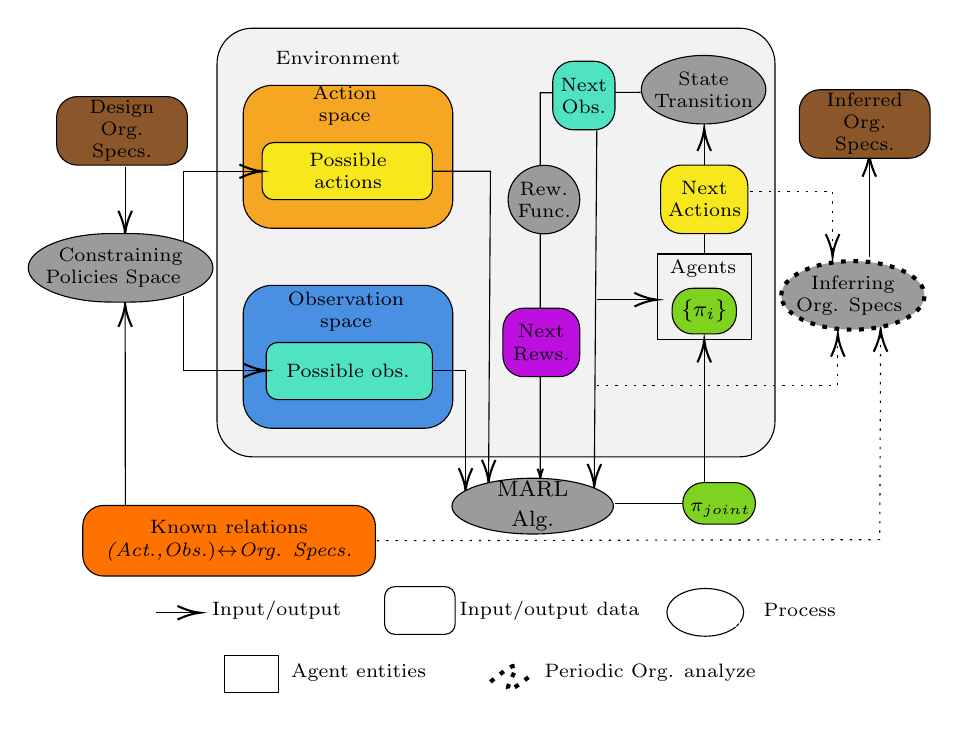
\begin{tikzpicture}[x=0.75pt,y=0.75pt,yscale=-1,xscale=1]
%uncomment if require: \path (0,1124); %set diagram left start at 0, and has height of 1124

%Shape: Rectangle [id:dp9937795244635512] 
\draw  [fill={rgb, 255:red, 242; green, 242; blue, 242 }  ,fill opacity=1 ] (108.97,721) .. controls (108.97,711.61) and (116.58,704) .. (125.97,704) -- (360.78,704) .. controls (370.17,704) and (377.78,711.61) .. (377.78,721) -- (377.78,893.49) .. controls (377.78,902.88) and (370.17,910.49) .. (360.78,910.49) -- (125.97,910.49) .. controls (116.58,910.49) and (108.97,902.88) .. (108.97,893.49) -- cycle ;
%Straight Lines [id:da6518751125509914] 
\draw    (335.62,932.92) -- (300.7,932.92) ;
%Straight Lines [id:da34207082497735786] 
\draw    (313,734.86) -- (264.7,735.09) -- (264.7,918.61) ;
\draw [shift={(264.7,920.61)}, rotate = 270] [color={rgb, 255:red, 0; green, 0; blue, 0 }  ][line width=0.75]    (4.37,-1.32) .. controls (2.78,-0.56) and (1.32,-0.12) .. (0,0) .. controls (1.32,0.12) and (2.78,0.56) .. (4.37,1.32)   ;
%Straight Lines [id:da9417034389402881] 
\draw    (343.7,754.18) -- (343.7,812.75) ;
\draw [shift={(343.7,752.18)}, rotate = 90] [color={rgb, 255:red, 0; green, 0; blue, 0 }  ][line width=0.75]    (10.93,-3.29) .. controls (6.95,-1.4) and (3.31,-0.3) .. (0,0) .. controls (3.31,0.3) and (6.95,1.4) .. (10.93,3.29)   ;
%Straight Lines [id:da4463435210078386] 
\draw    (343.7,922.88) -- (343.7,856.05) ;
\draw [shift={(343.7,854.05)}, rotate = 90] [color={rgb, 255:red, 0; green, 0; blue, 0 }  ][line width=0.75]    (10.93,-3.29) .. controls (6.95,-1.4) and (3.31,-0.3) .. (0,0) .. controls (3.31,0.3) and (6.95,1.4) .. (10.93,3.29)   ;
%Straight Lines [id:da8247669117759437] 
\draw    (291.96,834.78) -- (300.52,834.78) -- (318.99,834.78) ;
\draw [shift={(320.99,834.78)}, rotate = 180] [color={rgb, 255:red, 0; green, 0; blue, 0 }  ][line width=0.75]    (10.93,-3.29) .. controls (6.95,-1.4) and (3.31,-0.3) .. (0,0) .. controls (3.31,0.3) and (6.95,1.4) .. (10.93,3.29)   ;
%Rounded Rect [id:dp13052707912371297] 
\draw  [fill={rgb, 255:red, 245; green, 166; blue, 35 }  ,fill opacity=1 ] (121.59,745.3) .. controls (121.59,737.7) and (127.75,731.53) .. (135.35,731.53) -- (208.78,731.53) .. controls (216.39,731.53) and (222.55,737.7) .. (222.55,745.3) -- (222.55,786.6) .. controls (222.55,794.2) and (216.39,800.36) .. (208.78,800.36) -- (135.35,800.36) .. controls (127.75,800.36) and (121.59,794.2) .. (121.59,786.6) -- cycle ;
%Rounded Rect [id:dp7026077814365836] 
\draw  [fill={rgb, 255:red, 74; green, 144; blue, 226 }  ,fill opacity=1 ] (121.59,841.66) .. controls (121.59,834.06) and (127.75,827.89) .. (135.35,827.89) -- (208.78,827.89) .. controls (216.39,827.89) and (222.55,834.06) .. (222.55,841.66) -- (222.55,882.96) .. controls (222.55,890.56) and (216.39,896.72) .. (208.78,896.72) -- (135.35,896.72) .. controls (127.75,896.72) and (121.59,890.56) .. (121.59,882.96) -- cycle ;
%Rounded Rect [id:dp7429651229296941] 
\draw  [fill={rgb, 255:red, 248; green, 231; blue, 28 }  ,fill opacity=1 ] (130.7,764.57) .. controls (130.7,761.53) and (133.17,759.06) .. (136.21,759.06) -- (207.2,759.06) .. controls (210.24,759.06) and (212.7,761.53) .. (212.7,764.57) -- (212.7,781.09) .. controls (212.7,784.13) and (210.24,786.6) .. (207.2,786.6) -- (136.21,786.6) .. controls (133.17,786.6) and (130.7,784.13) .. (130.7,781.09) -- cycle ;
%Rounded Rect [id:dp2626666197665244] 
\draw  [fill={rgb, 255:red, 80; green, 227; blue, 194 }  ,fill opacity=1 ] (132.7,860.9) .. controls (132.7,857.86) and (135.17,855.39) .. (138.21,855.39) -- (207.2,855.39) .. controls (210.24,855.39) and (212.7,857.86) .. (212.7,860.9) -- (212.7,877.42) .. controls (212.7,880.46) and (210.24,882.92) .. (207.2,882.92) -- (138.21,882.92) .. controls (135.17,882.92) and (132.7,880.46) .. (132.7,877.42) -- cycle ;
%Straight Lines [id:da37906510942957117] 
\draw    (291.96,750.8) -- (290.72,922.92) ;
\draw [shift={(290.7,924.92)}, rotate = 270.41] [color={rgb, 255:red, 0; green, 0; blue, 0 }  ][line width=0.75]    (10.93,-3.29) .. controls (6.95,-1.4) and (3.31,-0.3) .. (0,0) .. controls (3.31,0.3) and (6.95,1.4) .. (10.93,3.29)   ;
%Straight Lines [id:da8878827995944159] 
\draw  [dash pattern={on 0.84pt off 2.51pt}]  (361.37,782.47) -- (405.54,782.47) -- (405.54,812.13) ;
\draw [shift={(405.54,814.13)}, rotate = 270] [color={rgb, 255:red, 0; green, 0; blue, 0 }  ][line width=0.75]    (10.93,-3.29) .. controls (6.95,-1.4) and (3.31,-0.3) .. (0,0) .. controls (3.31,0.3) and (6.95,1.4) .. (10.93,3.29)   ;
%Straight Lines [id:da8073435187842593] 
\draw  [dash pattern={on 0.84pt off 2.51pt}]  (291.96,876.08) -- (408.07,876.08) -- (408.07,853.3) ;
\draw [shift={(408.07,851.3)}, rotate = 90] [color={rgb, 255:red, 0; green, 0; blue, 0 }  ][line width=0.75]    (10.93,-3.29) .. controls (6.95,-1.4) and (3.31,-0.3) .. (0,0) .. controls (3.31,0.3) and (6.95,1.4) .. (10.93,3.29)   ;
%Straight Lines [id:da9521506867066192] 
\draw    (137.99,947.66) -- (64.8,947.66) -- (64.7,838.92) ;
\draw [shift={(64.7,836.92)}, rotate = 89.95] [color={rgb, 255:red, 0; green, 0; blue, 0 }  ][line width=0.75]    (10.93,-3.29) .. controls (6.95,-1.4) and (3.31,-0.3) .. (0,0) .. controls (3.31,0.3) and (6.95,1.4) .. (10.93,3.29)   ;
%Straight Lines [id:da8173351196218479] 
\draw  [dash pattern={on 0.84pt off 2.51pt}]  (177.06,950.92) -- (428.26,950.41) -- (428.69,850.92) ;
\draw [shift={(428.7,848.92)}, rotate = 90.25] [color={rgb, 255:red, 0; green, 0; blue, 0 }  ][line width=0.75]    (10.93,-3.29) .. controls (6.95,-1.4) and (3.31,-0.3) .. (0,0) .. controls (3.31,0.3) and (6.95,1.4) .. (10.93,3.29)   ;
%Straight Lines [id:da6053298376683525] 
\draw    (64.7,770.92) -- (64.7,800.92) ;
\draw [shift={(64.7,802.92)}, rotate = 270] [color={rgb, 255:red, 0; green, 0; blue, 0 }  ][line width=0.75]    (10.93,-3.29) .. controls (6.95,-1.4) and (3.31,-0.3) .. (0,0) .. controls (3.31,0.3) and (6.95,1.4) .. (10.93,3.29)   ;
%Straight Lines [id:da8641416537329594] 
\draw    (423.21,814.13) -- (423.21,766.57) ;
\draw [shift={(423.21,764.57)}, rotate = 90] [color={rgb, 255:red, 0; green, 0; blue, 0 }  ][line width=0.75]    (10.93,-3.29) .. controls (6.95,-1.4) and (3.31,-0.3) .. (0,0) .. controls (3.31,0.3) and (6.95,1.4) .. (10.93,3.29)   ;
%Shape: Rectangle [id:dp009612592743657444] 
\draw   (320.99,812.75) -- (366.42,812.75) -- (366.42,854.05) -- (320.99,854.05) -- cycle ;
%Shape: Boxed Line [id:dp9105440631185389] 
\draw    (79.7,985.61) -- (98.84,985.61) ;
\draw [shift={(100.84,985.61)}, rotate = 180] [color={rgb, 255:red, 0; green, 0; blue, 0 }  ][line width=0.75]    (10.93,-3.29) .. controls (6.95,-1.4) and (3.31,-0.3) .. (0,0) .. controls (3.31,0.3) and (6.95,1.4) .. (10.93,3.29)   ;
%Shape: Rectangle [id:dp18940852352890292] 
\draw   (112.7,1006.17) -- (138.7,1006.17) -- (138.7,1023.94) -- (112.7,1023.94) -- cycle ;
%Curve Lines [id:da6070406744312455] 
\draw [line width=1.5]  [dash pattern={on 1.69pt off 2.76pt}]  (240.7,1018.92) .. controls (271.17,993.71) and (230.78,1040.06) .. (261.24,1014.84) ;
%Straight Lines [id:da04181106466856366] 
\draw    (92.7,806.92) -- (92.7,772.92) -- (128.7,772.92) ;
\draw [shift={(130.7,772.92)}, rotate = 180] [color={rgb, 255:red, 0; green, 0; blue, 0 }  ][line width=0.75]    (10.93,-3.29) .. controls (6.95,-1.4) and (3.31,-0.3) .. (0,0) .. controls (3.31,0.3) and (6.95,1.4) .. (10.93,3.29)   ;
%Straight Lines [id:da5269327271789521] 
\draw    (92.7,832.92) -- (92.7,868.92) -- (130.7,868.92) ;
\draw [shift={(132.7,868.92)}, rotate = 180] [color={rgb, 255:red, 0; green, 0; blue, 0 }  ][line width=0.75]    (10.93,-3.29) .. controls (6.95,-1.4) and (3.31,-0.3) .. (0,0) .. controls (3.31,0.3) and (6.95,1.4) .. (10.93,3.29)   ;
%Straight Lines [id:da8384029096649059] 
\draw    (228.7,924.92) -- (228.7,868.92) -- (212.7,868.92) ;
\draw [shift={(228.7,926.92)}, rotate = 270] [color={rgb, 255:red, 0; green, 0; blue, 0 }  ][line width=0.75]    (10.93,-3.29) .. controls (6.95,-1.4) and (3.31,-0.3) .. (0,0) .. controls (3.31,0.3) and (6.95,1.4) .. (10.93,3.29)   ;
%Straight Lines [id:da8549749304566603] 
\draw    (212.7,772.92) -- (240.7,772.92) -- (239.8,920.92) ;
\draw [shift={(239.79,922.92)}, rotate = 270.35] [color={rgb, 255:red, 0; green, 0; blue, 0 }  ][line width=0.75]    (10.93,-3.29) .. controls (6.95,-1.4) and (3.31,-0.3) .. (0,0) .. controls (3.31,0.3) and (6.95,1.4) .. (10.93,3.29)   ;

% Text Node
\draw (177.2,1014.42) node  [font=\small] [align=left] {{\scriptsize Agent entities}};
% Text Node
\draw (317.7,1014.42) node  [font=\small] [align=left] {{\scriptsize Periodic Org. analyze}};
% Text Node
\draw    (189.7,978.02) .. controls (189.7,975.26) and (191.94,973.02) .. (194.7,973.02) -- (218.7,973.02) .. controls (221.46,973.02) and (223.7,975.26) .. (223.7,978.02) -- (223.7,991.02) .. controls (223.7,993.78) and (221.46,996.02) .. (218.7,996.02) -- (194.7,996.02) .. controls (191.94,996.02) and (189.7,993.78) .. (189.7,991.02) -- cycle  ;
\draw (206.7,984.52) node  [font=\small] [align=left] {\begin{minipage}[lt]{20.08pt}\setlength\topsep{0pt}
\begin{center}
\textcolor[rgb]{1,1,1}{{\tiny assaaaa}}
\end{center}

\end{minipage}};
% Text Node
\draw (269.2,984.42) node  [font=\small] [align=left] {{\scriptsize Input/output data}};
% Text Node
\draw (137.7,984.42) node  [font=\small] [align=left] {{\scriptsize Input/output}};
% Text Node
\draw    (325.7,985.42) .. controls (325.7,979.07) and (333.98,973.92) .. (344.2,973.92) .. controls (354.42,973.92) and (362.7,979.07) .. (362.7,985.42) .. controls (362.7,991.77) and (354.42,996.92) .. (344.2,996.92) .. controls (333.98,996.92) and (325.7,991.77) .. (325.7,985.42) -- cycle  ;
\draw (344.2,985.42) node  [font=\small] [align=left] {\begin{minipage}[lt]{22.12pt}\setlength\topsep{0pt}
\begin{center}
\textcolor[rgb]{1,1,1}{{\tiny aassssaa}}
\end{center}

\end{minipage}};
% Text Node
\draw (389.7,984.42) node  [font=\small] [align=left] {{\scriptsize Process}};
% Text Node
\draw  [fill={rgb, 255:red, 139; green, 87; blue, 42 }  ,fill opacity=1 ]  (31.7,746.92) .. controls (31.7,741.4) and (36.18,736.92) .. (41.7,736.92) -- (84.7,736.92) .. controls (90.22,736.92) and (94.7,741.4) .. (94.7,746.92) -- (94.7,759.92) .. controls (94.7,765.45) and (90.22,769.92) .. (84.7,769.92) -- (41.7,769.92) .. controls (36.18,769.92) and (31.7,765.45) .. (31.7,759.92) -- cycle  ;
\draw (63.2,753.42) node  [font=\scriptsize] [align=left] {\begin{minipage}[lt]{40.43pt}\setlength\topsep{0pt}
\begin{center}
Design\\Org. Specs.
\end{center}

\end{minipage}};
% Text Node
\draw  [fill={rgb, 255:red, 155; green, 155; blue, 155 }  ,fill opacity=1 ]  (249.21,786.55) .. controls (249.21,777.43) and (256.94,770.05) .. (266.46,770.05) .. controls (275.99,770.05) and (283.72,777.43) .. (283.72,786.55) .. controls (283.72,795.66) and (275.99,803.05) .. (266.46,803.05) .. controls (256.94,803.05) and (249.21,795.66) .. (249.21,786.55) -- cycle  ;
\draw (266.46,786.55) node  [font=\scriptsize,xslant=-0.02] [align=left] {\begin{minipage}[lt]{20.58pt}\setlength\topsep{0pt}
\begin{center}
Rew.\\Func.
\end{center}

\end{minipage}};
% Text Node
\draw (165.76,716.05) node  [font=\scriptsize] [align=left] {\begin{minipage}[lt]{42.81pt}\setlength\topsep{0pt}
\begin{center}
Environment
\end{center}

\end{minipage}};
% Text Node
\draw (170.49,741.51) node  [font=\scriptsize] [align=left] {\begin{minipage}[lt]{43.61pt}\setlength\topsep{0pt}
\begin{center}
Action space
\end{center}

\end{minipage}};
% Text Node
\draw (171.12,840.63) node  [font=\scriptsize] [align=left] {\begin{minipage}[lt]{62.26pt}\setlength\topsep{0pt}
\begin{center}
Observation space
\end{center}

\end{minipage}};
% Text Node
\draw (172.07,772.83) node  [font=\scriptsize] [align=left] {\begin{minipage}[lt]{54.32pt}\setlength\topsep{0pt}
\begin{center}
Possible actions
\end{center}

\end{minipage}};
% Text Node
\draw (172.07,869.19) node  [font=\scriptsize] [align=left] {\begin{minipage}[lt]{45.19pt}\setlength\topsep{0pt}
\begin{center}
Possible obs.
\end{center}

\end{minipage}};
% Text Node
\draw  [fill={rgb, 255:red, 155; green, 155; blue, 155 }  ,fill opacity=1 ]  (261.04, 934.24) circle [x radius= 38.89, y radius= 13.44]   ;
\draw (261.04,934.24) node  [font=\small] [align=left] {\begin{minipage}[lt]{37.13pt}\setlength\topsep{0pt}
\begin{center}
{\footnotesize MARL Alg.}
\end{center}

\end{minipage}};
% Text Node
\draw  [fill={rgb, 255:red, 126; green, 211; blue, 33 }  ,fill opacity=1 ]  (333.36,932.92) .. controls (333.36,927.4) and (337.84,922.92) .. (343.36,922.92) -- (358.36,922.92) .. controls (363.88,922.92) and (368.36,927.4) .. (368.36,932.92) .. controls (368.36,938.45) and (363.88,942.92) .. (358.36,942.92) -- (343.36,942.92) .. controls (337.84,942.92) and (333.36,938.45) .. (333.36,932.92) -- cycle  ;
\draw (350.86,932.92) node  [font=\scriptsize] [align=left] {\begin{minipage}[lt]{20.95pt}\setlength\topsep{0pt}
\begin{center}
$\displaystyle \pi _{joint}$
\end{center}

\end{minipage}};
% Text Node
\draw  [fill={rgb, 255:red, 155; green, 155; blue, 155 }  ,fill opacity=1 ]  (313.39,733.6) .. controls (313.39,724.48) and (326.82,717.1) .. (343.39,717.1) .. controls (359.96,717.1) and (373.39,724.48) .. (373.39,733.6) .. controls (373.39,742.71) and (359.96,750.1) .. (343.39,750.1) .. controls (326.82,750.1) and (313.39,742.71) .. (313.39,733.6) -- cycle  ;
\draw (343.39,733.6) node  [font=\scriptsize] [align=left] {\begin{minipage}[lt]{37.77pt}\setlength\topsep{0pt}
\begin{center}
State\\Transition \ 
\end{center}

\end{minipage}};
% Text Node
\draw  [fill={rgb, 255:red, 189; green, 16; blue, 224 }  ,fill opacity=1 ]  (246.7,848.88) .. controls (246.7,843.35) and (251.18,838.88) .. (256.7,838.88) -- (273.7,838.88) .. controls (279.22,838.88) and (283.7,843.35) .. (283.7,848.88) -- (283.7,861.88) .. controls (283.7,867.4) and (279.22,871.88) .. (273.7,871.88) -- (256.7,871.88) .. controls (251.18,871.88) and (246.7,867.4) .. (246.7,861.88) -- cycle  ;
\draw (265.2,855.38) node  [font=\scriptsize] [align=left] {\begin{minipage}[lt]{22.57pt}\setlength\topsep{0pt}
\begin{center}
Next\\Rews.
\end{center}

\end{minipage}};
% Text Node
\draw  [fill={rgb, 255:red, 255; green, 114; blue, 0 }  ,fill opacity=1 ]  (44.27,943.92) .. controls (44.27,938.4) and (48.75,933.92) .. (54.27,933.92) -- (175.27,933.92) .. controls (180.79,933.92) and (185.27,938.4) .. (185.27,943.92) -- (185.27,957.92) .. controls (185.27,963.45) and (180.79,967.92) .. (175.27,967.92) -- (54.27,967.92) .. controls (48.75,967.92) and (44.27,963.45) .. (44.27,957.92) -- cycle  ;
\draw (114.77,950.92) node  [font=\scriptsize] [align=left] {\begin{minipage}[lt]{93.15pt}\setlength\topsep{0pt}
\begin{center}
Known relations\\\textit{(Act.,Obs.})$\displaystyle \leftrightarrow $\textit{Org. Specs.}
\end{center}

\end{minipage}};
% Text Node
\draw  [fill={rgb, 255:red, 155; green, 155; blue, 155 }  ,fill opacity=1 ]  (18,819.42) .. controls (18,810.31) and (35.91,802.92) .. (58,802.92) -- (67,802.92) .. controls (89.09,802.92) and (107,810.31) .. (107,819.42) .. controls (107,828.54) and (89.09,835.92) .. (67,835.92) -- (58,835.92) .. controls (35.91,835.92) and (18,828.54) .. (18,819.42) -- cycle  ;
\draw (62.5,819.42) node  [font=\scriptsize] [align=left] {\begin{minipage}[lt]{57.49pt}\setlength\topsep{0pt}
\begin{center}
Constraining\\Policies Space \ \ \ 
\end{center}

\end{minipage}};
% Text Node
\draw  [fill={rgb, 255:red, 80; green, 227; blue, 194 }  ,fill opacity=1 ]  (270.7,729.92) .. controls (270.7,724.4) and (275.18,719.92) .. (280.7,719.92) -- (290.7,719.92) .. controls (296.22,719.92) and (300.7,724.4) .. (300.7,729.92) -- (300.7,742.92) .. controls (300.7,748.45) and (296.22,752.92) .. (290.7,752.92) -- (280.7,752.92) .. controls (275.18,752.92) and (270.7,748.45) .. (270.7,742.92) -- cycle  ;
\draw (285.7,736.42) node  [font=\scriptsize] [align=left] {\begin{minipage}[lt]{17.81pt}\setlength\topsep{0pt}
\begin{center}
Next\\Obs.
\end{center}

\end{minipage}};
% Text Node
\draw (343.14,819.98) node  [font=\scriptsize] [align=left] {\begin{minipage}[lt]{24.96pt}\setlength\topsep{0pt}
\begin{center}
Agents
\end{center}

\end{minipage}};
% Text Node
\draw  [fill={rgb, 255:red, 126; green, 211; blue, 33 }  ,fill opacity=1 ]  (328.2,839.28) .. controls (328.2,833.76) and (332.68,829.28) .. (338.2,829.28) -- (349.2,829.28) .. controls (354.73,829.28) and (359.2,833.76) .. (359.2,839.28) -- (359.2,841.28) .. controls (359.2,846.81) and (354.73,851.28) .. (349.2,851.28) -- (338.2,851.28) .. controls (332.68,851.28) and (328.2,846.81) .. (328.2,841.28) -- cycle  ;
\draw (343.7,840.28) node  [font=\footnotesize] [align=left] {\begin{minipage}[lt]{18.45pt}\setlength\topsep{0pt}
\begin{center}
$\displaystyle \{\pi _{i}\}$
\end{center}

\end{minipage}};
% Text Node
\draw  [fill={rgb, 255:red, 248; green, 231; blue, 28 }  ,fill opacity=1 ]  (322.7,779.92) .. controls (322.7,774.4) and (327.18,769.92) .. (332.7,769.92) -- (354.7,769.92) .. controls (360.22,769.92) and (364.7,774.4) .. (364.7,779.92) -- (364.7,792.92) .. controls (364.7,798.45) and (360.22,802.92) .. (354.7,802.92) -- (332.7,802.92) .. controls (327.18,802.92) and (322.7,798.45) .. (322.7,792.92) -- cycle  ;
\draw (343.7,786.42) node  [font=\scriptsize] [align=left] {\begin{minipage}[lt]{26.14pt}\setlength\topsep{0pt}
\begin{center}
Next\\Actions
\end{center}

\end{minipage}};
% Text Node
\draw  [color={rgb, 255:red, 0; green, 0; blue, 0 }  ,draw opacity=1 ][fill={rgb, 255:red, 155; green, 155; blue, 155 }  ,fill opacity=1 ][dash pattern={on 1.69pt off 2.76pt}][line width=1.5]   (380.82,832.71) .. controls (380.82,823.6) and (396.27,816.21) .. (415.32,816.21) .. controls (434.38,816.21) and (449.82,823.6) .. (449.82,832.71) .. controls (449.82,841.82) and (434.38,849.21) .. (415.32,849.21) .. controls (396.27,849.21) and (380.82,841.82) .. (380.82,832.71) -- cycle  ;
\draw (415.32,832.71) node  [font=\scriptsize] [align=left] {\begin{minipage}[lt]{44.39pt}\setlength\topsep{0pt}
\begin{center}
Inferring\\Org. Specs \ \ 
\end{center}

\end{minipage}};
% Text Node
\draw  [fill={rgb, 255:red, 139; green, 87; blue, 42 }  ,fill opacity=1 ]  (389.5,743.62) .. controls (389.5,738.09) and (393.98,733.62) .. (399.5,733.62) -- (442.5,733.62) .. controls (448.02,733.62) and (452.5,738.09) .. (452.5,743.62) -- (452.5,756.62) .. controls (452.5,762.14) and (448.02,766.62) .. (442.5,766.62) -- (399.5,766.62) .. controls (393.98,766.62) and (389.5,762.14) .. (389.5,756.62) -- cycle  ;
\draw (421,750.12) node  [font=\scriptsize] [align=left] {\begin{minipage}[lt]{40.43pt}\setlength\topsep{0pt}
\begin{center}
Inferred\\Org. Specs.
\end{center}

\end{minipage}};


\end{tikzpicture}
  \caption{Une vue récapitulative du processus PRAHOM}
  \label{fig:prahom_process}
\end{figure}

\subsubsection{Processus 1 : Déduire des spécifications organisationnelles}

Plutôt que d'utiliser directement les politiques conjointes, nous utilisons les historiques conjoints, car ils peuvent être construits avec les actions résultantes observées lorsque les observations sont reçues au cours d'une série d'épisodes de test. En effet, pour une politique donnée $\pi \in \Pi$, l'historique associé est par définition $h \in h_{joint} = \langle(\omega_k,a_k) | k \in \mathbb{N}\rangle$ et le $(\omega_k,a_k) \in \pi$.
Ensuite, en raison de la difficulté de déduire des informations liées aux spécifications organisationnelles, il est possible d'associer des séquences de couples observation-action aux spécifications de l'organisation sous la forme d'une relation \textquote{plusieurs à plusieurs}. Cela met en place un premier cadre d'identification des spécifications organisationnelles dans les historiques. Le reste de cette section aborde cette difficulté.

Le concepteur peut définir certaines relations entre les spécifications $\mathcal{M}OISE^+$ et les historiques conjoints. Leurs prémisses viennent du fait que certaines spécifications du modèle organisationnel $\mathcal{M}OISE^+$ peuvent être mappées à des sous-ensembles d'actions d'une seule politique commune sous-optimale.
À partir de ces relations, il est possible d'utiliser des approches empiriques ou statistiques pour déduire des spécifications organisationnelles à partir d'historiques communs.
%JS
%JPJ je te laisse reprendre au besoin. Penser a dire (si ce n'est pas fait) dans les perspective qu'il faudra lever cette hypothese -> Ça me va
Pour simplifier l'étude, nous ne considérons dans un premier temps qu'un seul groupe d'agents et nous ne prenons donc pas en compte les inter-liens et les inter-compatibilités. De même, nous ne considérons qu'un seul schéma social.
Premièrement, nous examinons le niveau individuel en essayant de comprendre les rôles, les liens, les sous-groupes, les objectifs individuels, les missions et les plans joués par les agents en échantillonnant les sous-séquences historiques $h \in H$ et en les comparant avec les sous-séquences historiques connues afin de déterminer des rôles.

Après avoir analysé plusieurs politiques conjointes, le processus tente de renforcer une vision globale des objectifs, des missions, des plans et de la connaissance de la mission par rapport à l'objectif ; avec les informations partiellement déduites au niveau individuel.
Au final, notre processus tente de synthétiser les connaissances inférées jusqu'à avoir une meilleure vision de la cardinalité des agents par sous-groupe, de la cardinalité des agents pour chaque mission, de la cardinalité des rôles, des compatibilités entre rôles, des autorisations et des obligations.

\subsubsection{Processus 2 : Contraindre l'espace des politiques}

Nous considérons un algorithme MARL donné qui converge itérativement vers une politique commune de sorte que la politique de chaque agent soit mise à jour à chaque étape jusqu'à un horizon fini.
Nous privilégions l'algorithme \emph{Proximal Policy Optimization} (PPO) pour son efficacité prouvée dans des environnements multi-agents coopératifs sans nécessiter de modifications algorithmiques ou d'architectures spécifiques au domaine~\cite{Yu2022}.
Pour contraindre les politiques conjointes possibles à celles satisfaisant les spécifications organisationnelles de conception $os_{init}$, nous proposons de contraindre les ensembles d'actions et d'observations pour chaque agent en fonction de $os_{init}$ à chaque étape. Par exemple, nous pouvons contraindre un agent à converger vers un rôle donné en interdisant les actions liées à d'autres rôles. Nous utilisons cette idée pour mettre en place notre processus visant à guider l'entrainement en fonction des contraintes organisationnelles de conception.

Dans un premier temps, nous utilisons les relations précédemment établies entre spécifications organisationnelles et couples action-observation, pour déterminer les actions autorisées ou interdites jouables par les agents à chaque étape.
Ensuite, le procesus calcule l'ensemble d'actions autorisées $A_{step}$ en fonction de l'historique actuel $h_{joint,i}$. Ensuite, une action est choisie parmi les actions autorisées. Cette action $a_{step} \in A_{step}$ est ajoutée à l'historique pour être utilisée pour mettre à jour la politique de l'agent à l'étape suivante. Ensuite, l'algorithme MARL met à jour la politique commune, donc les politiques des agents, avec l'action et l'observation en cours.
Enfin, une analyse de la politique conjointe sous-optimale actuelle $\pi_{joint}$ satisfaisant $os_{init}$ est déclenchée périodiquement. Le processus améliore de manière itérative l'efficacité des politiques conjointes et l'exactitude des spécifications organisationnelles qui en découlent.
Nous pouvons noter que la restriction impliquée par $os_{init}$ dans les éventuelles politiques conjointes pourrait empêcher l'algorithme MARL de trouver une politique commune qui satisfasse la récompense cumulative minimale attendue définie par le concepteur.

\subsection{Outil d'ingénierie}

%%%%%%%% DEBUT DES MODIFICATIONS %%%%%%%%%%%%%%
Dans le cadre de CybMASDE\footnotemark[1]
%
\footnotetext[1]{\emph{Cyberdefense Multi Agent System Developpment Environment} est un simulateur pour SMA de Cyberdéfense et disponible à \url{https://github.com/julien6/CybMASDE}}
%
, nous proposons \emph{PRAHOM Wrapper}\label{PettingZoo-wrapper} comme outil augmentant la bibliothèque \emph{PettingZoo} qui fournit une API standardisée pour le développement d'environnements et l'application d'algorithmes MARL.
%
\emph{PRAHOM Wrapper} fournit des moyens d'inférer des spécifications organisationnelles à partir d'agents entraînés ou contraindre leur entraînement.
% Lors de l'entraînement, des actions/observations sont masquées ou mis en avant pour contraindre l'apprentissage d'un agent selon les spécifications organisationnelles données.
%
\autoref{lst:wrapper_basic_use} présente une utilisation simple du wrapper pour augmenter un environnement \emph{PettingZoo} (ligne 5) avec des relations connues entre les spécifications organisationnelles et les historiques attendus (ligne 3) ainsi que les spécifications organisationnelles qui contraignent les politiques possibles des agents (ligne 4).

Ici, l'entrainement est effectué avec une fonctionnalité de \emph{PRAHOM Wrapper} qui utilise PPO et la configuration par défaut (ligne 6).
Pendant l'entrainement, \textquote{agent\_0} est contraint au rôle \textquote{follower}. Ainsi ses actions doivent être choisies d'après les historiques attendus (exprimables de diverses façons en plus de listes). Ces contraintes peuvent être satisfaites selon trois modes disponibles : i) masquer/corriger de façon externe aux politiques les observations reçues et actions choisies  ; ii) enseigner les contraintes aux politiques courantes ; iii) modifier en interne les politiques pour respecter les contraintes.

Après entrainement, \emph{PRAHOM Wrapper} infère les spécifications organisationnelles à partir de plusieurs historiques conjoints (lié chacun à un épisode) ; ainsi que l'instanciation de l'organisation généralisée pour chaque historique conjoint (ligne 7).
Ce processus d'inférence utilise d'abord les relations connues entre les historiques et les spécifications organisationnelles (ligne 3) : l'historique d'un agent qui contient l'observation $14$ (\textquote{commande reçue}) et l'action $74$ (\textquote{appliquer l'ordre}), est un \textquote{follower}. De même, pour les liens entre les rôles en utilisant des expressions régulières pour les historiques (ligne 3).
%
Ensuite, en s'appuyant sur la définition donnée de chaque spécification organisationnelle vis-à-vis des historiques, \emph{PRAHOM Wrapper} généralise plusieurs historiques conjoints.
% pour obtenir de nouvelles spécifications organisationnelles.
%
Par exemple, un rôle est obtenu en mesurant la similarité entre des historiques. Cela peut être fait de plusieurs manières : clustering de séquences (avec un dendrogramme) ; K-voisins les plus proches (avec ACP des historiques) ; analyse statistique (en particulier, fréquence d'action dans diverses visualisations) ; etc.

À partir des premières spécifications organisationnelles obtenues, un algorithme proposé déduit empiriquement d'autres spécifications organisationnelles telles que les compatibilités.
Ces résultats peuvent être incomplets ou bruités en raison des limites des techniques et de l'algorithme d'inférence des spécifications organisationnelles. Cependant, les résultats étant conformes à $\mathcal{M}OISE^+$, ils peuvent aider à la conception SMA à la lumière des spécifications organisationnelles proposées.
%%%%%%%% FIN DES MODIFICATIONS %%%%%%%%%%%%%%

\begin{lstlisting}[language=Python, caption={Utilisation basique de \emph{PRAHOM Wrapper}}, label={lst:wrapper_basic_use}]
from omarl_experiments import prahom_wrapper
env=PettingZoo_env.parallel_env(render_mode="human")
specs_to_hist={"structural_specifications":{"roles":{"follower":{"23":41,"14":[74,0]}}...},"functional_specifications":{"links":{"(leader,follower,aut)":".*14.*?89"}...}...}
policy_specs_constr={"agent_0":{"structural_specifications":"roles":["follower"]}}
env=prahom_wrapper(env,action_to_specs,training_specs)
env.train("default_PPO")
trained_specs,agent_to_specs=env.prahom_specs()
\end{lstlisting}

% =============

% \begin{itemize}
% \item Questions au niveau du système multi-agents (approche centrée sur le système)
% \begin{itemize}
% \item Nombre d'agents, quelle hétérogénéité ?
% \item Quel est le support commun (Environnement) partagé par les agents ?
% \item Quels mécanismes de communication sont disponibles pour les agents ?
% \item Quels sont les langages de communication, les ontologies, les protocoles d'interaction utilisés par les agents ?
% \item Quelle est l'organisation au sein de laquelle les agents opèrent ? Comment est-il établi ?
% \item Comment les agents coordonnent-ils leurs actions ? Comment assurer un fonctionnement cohérent ?
% \end{itemize}

% \item Questions au niveau de l'agent (approche centrée sur l'agent)
% \begin{itemize}
% \item Que représente un agent ? Quelles actions doivent être encapsulées dans un agent ?
% \item Comment les agents représentent-ils l'environnement et l'organisation dans lesquels ils opèrent ?
% \item Comment les agents gèrent-ils les interactions avec d'autres agents ?
% \item Quelle est la structure interne des agents ?
% \end{itemize}
% \end{itemize}

% ================================================== =================================================== =

\section{Évaluation dans des environnements de jeu coopératif}

% Évaluation
% Afin de vérifier et démontrer l'approche, est appliquée sur l'étude de cas suivante.
% 	Étude de cas

\subsection{Protocole expérimental}

Afin d'évaluer AOMEA, nous utilisons PRAHOM dans des environnements simulés disponibles composés d'agents devant atteindre un objectif avec les meilleures performances à travers diverses stratégies collectives. Ces exemples présentent aussi l'avantage d'être facilement compréhensibles.
Nous avons sélectionné trois environnements de type Atari pour leur rendu visuel qui constitue un moyen pratique d'évaluer les résultats avec des observations manuelles\footnotemark[2].
Considérant la recherche sur les AICA, nous avons également considéré un environnement de Cyberdéfense comme une première tentative d'application de PRAHOM dans un environnement de Cyberdéfense non "visuel" :

\footnotetext[2]{Des explications supplémentaires et les exemples discutés utilisant le \emph{PRAHOM Wrapper} sont disponibles sur \url{https://github.com/julien6/omarl_experiments?tab=readme-ov-file\#predator-prey-with-communication}}

\begin{itemize}
  \item \textquote{Drone swarm - 3rd CAGE Challenge}~\cite{cage_challenge_3_announcement} (CYB) se compose d'agents cyber-défenseurs déployés sur des drones en réseau essayant de lutter contre les programmes malware déployés de manière malveillante. Nous pouvons nous attendre à ce que les agents \allowbreak isolent collectivement les drones compromis ;
  \item \textquote{Pistonball} (PBL)~\cite{Terry2021} se compose d'une série de pistons pour amener une balle de droite à gauche, nécessitant ainsi la représentation des voisins ;
  \item \textquote{Predator-prey with communication}~\cite{Lowe2017} (PPY) se compose de prédateurs surveillés par un leader pour mieux attraper des proies plus rapides, nécessitant ainsi des stratégies de chasse collectives ;
  \item \textquote{Knights Archers Zombies}~\cite{Terry2021} (KAZ) consiste en trois chevaliers et deux archers apprenant à tuer le plus de zombies, ce qui nécessite ainsi un positionnement spatial efficace des agents.
\end{itemize}

Nous avons appliqué AOMEA dans trois cas :
\begin{itemize}
  \item Pas de spécifications organisationnelles (NTS) : les agents doivent apprendre les stratégies collectives les plus efficaces sans aucune contrainte ni indication.
  \item Spécifications organisationnelles partiellement contraignantes (PTS) : certaines contraintes ou indications sont données pour aider à converger plus rapidement ou à répondre à des exigences.
  \item Spécifications organisationnelles entièrement contraignantes (FTS) : des politiques conjointes élaborées manuellement sont données, car elles constituent une référence concernant les politiques conjointes apprises.
\end{itemize}

\

\noindent Ici, nous ne présentons pas le détail des contraintes données dans NTS et FTS (disponibles dans le référentiel Git\footnotemark[2]).
%
\begin{figure*}[h!]
  \centering
  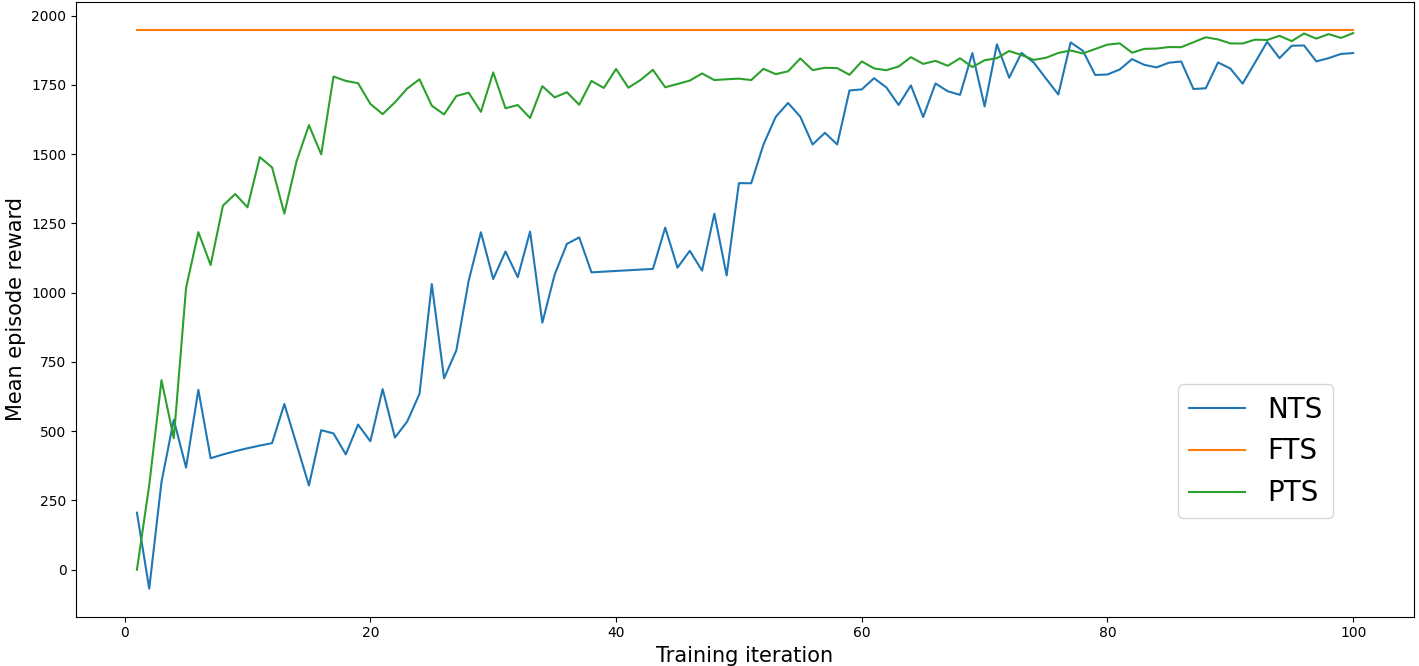
\includegraphics[width=0.76\linewidth]{figures/prahom_learning_curve.png}
  \caption{Récompense moyenne pour chaque itération dans l'environnement PBL pour les cas NTS, PTS et FTS}
  \label{fig:prahom_learning_curve}
\end{figure*}
%
\begin{figure*}[h!]
  \centering
  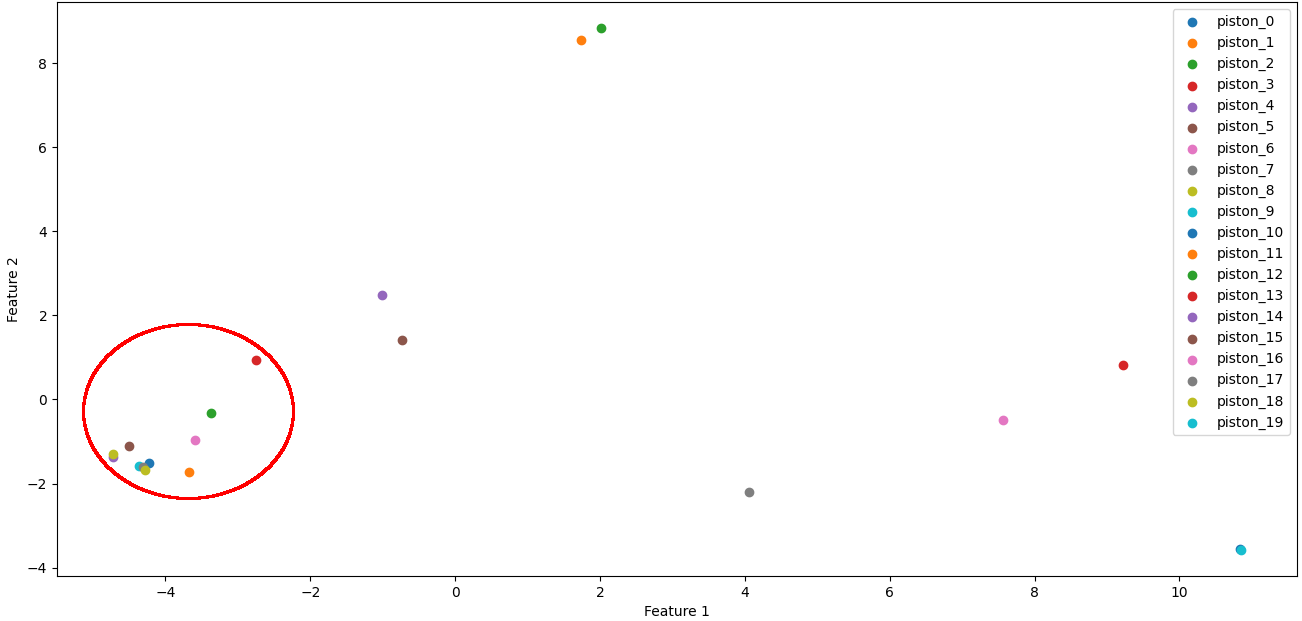
\includegraphics[width=0.75\linewidth]{figures/prahom_pca_analysis.png}
  \caption{ACP des historiques des agents entrainés dans l'environnement PBL}
  \label{fig:prahom_pca_analysis}
\end{figure*}
%
Nous évaluons dans le \autoref{tab:training_AOMEA_results}, l'impact de PRAHOM sur les critères suivants : les ratios de temps de convergence entre PTS, NTS et FTS pour atteindre un seuil de récompense cumulée. La stabilité est le rapport entre la moyenne des récompenses cumulées sur la récompense maximale après plusieurs épisodes. La stabilité des performances montre si les agents atteignent l'objectif de façon générale en évaluant plusieurs environnements générés avec différents paramètres.

\begin{table}[t!]

    \centering

    \begin{tblr}{colspec={llll},rows={m},measure=vbox,stretch=-1}

        \textbf{Environment} & \textbf{PTS/NTS} & \textbf{PTS/FTS} & \textbf{Perf. stability \\ (avg. / max)} \\

        \hline

        { PPL }
        & { 4.7 }
        & { 1.3 }
        & { 0.9 } \\

        \hline[dashed]

        { PPY }
        & { 6.3 }
        & { 2.2 }
        & { 0.78 } \\

        \hline[dashed]

        { KAZ }
        & { 4.0 }
        & { 1.1 }
        & { 0.42 } \\

        \hline[dashed]

        { CYB }
        & { 12 }
        & { 3.3 }
        & { 0.36 } \\


    \end{tblr}

    \caption{View of the AOMEA approach impact during training}

    \label{tab:training_AOMEA_results}

\end{table}


\subsection{Analyse}

La la \autoref{fig:prahom_learning_curve} montre l'évolution de la récompense dans les cas NTS, FTS et PTS pour l'environnement PBL. De manière générale, on peut remarquer que le temps de convergence est plus long pour NTS que pour PTS qui est également plus long que pour FTS. On constate, comme attendu, que l'espace de recherche diminuant, le temps de convergence est raccourci. Par exemple, nous remarquons une convergence plus rapide vers une solution sous-optimale dans l'environnement PBL en fournissant des spécifications organisationnelles. Bien que le PTS converge plus rapidement que le NTS vers une récompense cumulée comparable, le NTS peut surpasser le PTS parce que les politiques des agents entrainés sont conçues sur mesure pour résoudre le problème de manière beaucoup plus fine que ne peuvent les spécifications organisationnelles du concepteur. La faible stabilité des performances de l'environnement CYB indique que les agents ont des difficultés à trouver des stratégies générales à la différence des agents des autres environnements.

Nous prenons également en compte les critères suivants après l'entrainement : rôles, liens et performance globale. Une analyse qualitative est présentée dans le \autoref{tab:trained_AOMEA_results}
%
\begin{table}[t!]

    \centering

    \begin{tblr}{colspec={llll},rows={m},measure=vbox,stretch=-1}

        \textbf{Environment} & \textbf{Roles} & \textbf{Links} & \textbf{Global performance} \\

        \hline

        { 1 }
        & {  }
        & {  } \\
        & {  } \\

        \hline[dashed]

        { 2 }
        & {  }
        & {  } \\
        & {  } \\

        \hline[dashed]

        { 3 }
        & {  }
        & {  } \\
        & {  } \\

        \hline[dashed]

        { 4 }
        & {  }
        & {  } \\
        & {  } \\

        \hline[dashed]

        { 5 }
        & {  }
        & {  } \\
        & {  } \\

    \end{tblr}

    \caption{View of the OOMARL approach impact after training}

    \label{tab:trained_OOMARL_results}

\end{table}

%
% //TODO : schémas Moise+ et comparaison avec ceux attendus
%
Pour l'environnement PBL, les historiques des agents entrainés sont proches. Cela est visible dans l'ACP présentée à la \autoref{fig:prahom_pca_analysis} générée en exprimant les historiques des agents sous forme de vecteurs contenant les couples observation-action. Nous pouvons remarquer que l'historique de la plupart des agents se trouve dans la zone inférieure gauche (encerclée en rouge). Cela montre que la plupart des pistons semblent agir d'une façon similaire qu'on peut associer à un rôle. Nous ne pouvons déterminer aucune autre spécification organisationnelle en raison de l'absence de communication entre agents. Pour l'environnement KAZ, on peut remarquer deux rôles distincts : les archers ont tendance à s'éloigner des zombies, tandis que les chevaliers ont tendance à s'en approcher. Pour l'environnement PPY, nous pouvons observer que les spécifications de sortie indiquent des liens d'autorité entre le prédateur leader et les prédateurs simples pour permettre des stratégies collectives pour encercler les proies. Enfin, l'environnement CYB montre que les communications entre agents bleus permettent essentiellement d'isoler les drones suspectés ou de tenter de les réparer.

Pour l'environnement CYB, nous avons développé notre SMA raffiné via un simple arbre de décision élaboré à la main tel que préconisé dans AOMEA à la lumière des spécifications organisationnelles que nous obtenons en supprimant le bruit. Notre approche ne suggère pas de rôles généraux, mais des modèles stratégiques pertinents ont été identifiés. Par exemple, concernant les liens entre les rôles des agents, nous remarquons que les agents qui envoient des messages semblent fréquemment repérés comme suspects par leurs voisins. De plus, un agent cyber-défenseur se trouvant dans le rayon de communication d'un drone suspecté a tendance à couper sa communication et à la réactiver par la suite. Même si ces informations sont peu nombreuses, le score moyen que nous obtenons avec notre SMA raffiné est d'environ -2000, ce qui est en effet proche des 5 meilleurs scores sur les 20 participants. Cela montre l'applicabilité d'AOMEA au contexte de la Cyberdéfense.

\section{Conclusion}

% Dans cet article, nous avons présenté AOMEA, une nouvelle approche générale de conception SMA qui vise à faciliter la conception SMA lorsqu'elle ne peut pas être facilement réalisée par les concepteurs dans des environnements de déploiement très complexes.
Les méthodes multi-agents s'appuient sur les connaissances du concepteur pour concevoir une organisation SMA adaptée, mais ne fournissent pas de moyens automatiques pour déterminer les mécanismes organisationnels pertinents.
% uniquement à partir des exigences de conception et de l'objectif global.
Les techniques MARL ont été appliquées avec succès pour entrainer automatiquement des agents à atteindre un objectif donné sans caractérisation explicite des stratégies collectives émergentes.
L'originalité d'AOMEA est d'enrichir un processus MARL d'un modèle organisationnel explicite vers un objectif méthodologique pour aborder ces problématiques. Nous avons d'abord exposé comment AOMEA est destiné à être utilisé dans l'ingénierie SMA en tant qu'outil supplémentaire pour aider au processus de conception.
Ensuite, nous avons proposé de lier les politiques des agents (modélisées dans un Dec-POMDP) avec $\mathcal{M}OISE^+$ à travers le processus PRAHOM qui est au cœur d'AOMEA. Sous les conditions simplificatrices d'un groupe et d'un schéma social unique, PRAHOM permet de déterminer partiellement les spécifications organisationnelles à partir des historiques conjoints et de contraindre l'entrainement des politiques par rapport à des spécifications organisationnelles.
De plus, nous avons implémenté le wrapper \emph{PRAHOM PettingZoo} comme preuve de concept pour appliquer AOMEA.
Enfin, nous avons appliqué notre approche dans quatre environnements \emph{PettingZoo} pour évaluer l'impact pendant et après l'entrainement. Les performances obtenues se révèlent comparables à celles connues.

Même si PRAHOM est agnostique à l'égard de l'algorithme MARL, car il utilise l'historique des agents pour déduire des spécifications organisationnelles, reconstruire a posteriori les comportements collectifs des agents peut s'avérer difficile. En effet, une perspective pour PRAHOM est approfondir l'utilisation de techniques d'apprentissage non supervisé en plus des approches statistiques empiriques pour identifier des spécifications organisationnelles pertinentes à partir d'historiques conjoints. De plus, les travaux issus de l'apprentissage hiérarchique peuvent contribuer à mieux caractériser les stratégies émergentes durant l'apprentissage.
%À terme, nous visons également à améliorer l'applicabilité d'AOMEA en développant des interfaces dédiées construites autour de PRAHOM le rendant plus accessible aux contextes industriels et de recherche.

% % \usepackage{physics}
% \usepackage{tikz}
% \usepackage{amsmath}
% \usepackage{mathdots}
% % \usepackage{yhmath}
% \usepackage{cancel}
% \usepackage{color}
% \usepackage{siunitx}
% \usepackage{array}
% \usepackage{multirow}
% % \usepackage{amssymb}
% \usepackage{gensymb}
% \usepackage{tabularx}
% \usepackage{extarrows}
% \usepackage{booktabs}
% \usetikzlibrary{fadings}
% \usetikzlibrary{patterns}
% \usetikzlibrary{shadows.blur}
% \usetikzlibrary{shapes}
% % ---------

% \usepackage{amssymb}
% \usepackage{csquotes}
% \usepackage[export]{adjustbox}

% \usepackage{tabularray}\UseTblrLibrary{varwidth}
% \usepackage{xcolor}
% \def\BibTeX{{\rm B\kern-.05em{\sc i\kern-.025em b}\kern-.08em
%     T\kern-.1667em\lower.7ex\hbox{E}\kern-.125emX}}
% \usepackage{amsmath}
% \newcommand{\probP}{\text{I\kern-0.15em P}}

% \newcommand{\myCustomSize}[1]{%
%   \fontsize{9}{10.8}\selectfont
%   #1
% }


\section{Introduction}

\footnotetext[1]{Cet article est traduit d'un papier long acceptée à AAMAS~\cite{soule2025moisemarl}.}

% Contexte  
L'apprentissage par renforcement multi-agent~\cite{maisonhaute2024} (\textit{Multi-Agent Reinforcement Learning - MARL}) permet de trouver une politique conjointe qui régit les actions individuelles des agents et leurs interactions pour atteindre un objectif sans gérer explicitement leur coordination. Dans des environnements nécéssitant des interactions sociales, les agents peuvent aboutir à des comportements semblables à des rôles et objectifs implicites, qui les rapprochent en partie d'une \textbf{organisation} (structurelle et fonctionnelle) telle que décrite dans $\mathcal{M}OISE^+$~\cite{Hubner2007}.

% Problématique
Toutefois, l’identification de ces rôles et objectifs émergents reste complexe en raison de comportements souvent bruités ou irréguliers. Afin d’interpréter des comportements comme des rôles et objectifs d'une organisation implicite, nous introduisons l’\textbf{adéquation organisationnelle}.
Ce concept propose une vision organisationnelle pour envisager deux problèmes encore peu explorés que sont le controle et l'explicabilité dans le MARL au travers de:
i) \textbf{L'évaluation de l'adéquation organisationnelle} consiste à mesurer l'alignement d'une politique conjointe avec une organisation explicite où les comportements sont réguliers. La littérature, souvent centrée sur les rôles~\cite{Isakov2024, Wen2024, Xie2024}, manque d'approches systématiques dotées de moyens quantitatifs
 ; \quad
ii) \textbf{Le contrôle de l'adéquation organisationnelle} consiste à orienter les agents vers des politiques conformes à une organisation via des contraintes ou incitations définies. Ce contrôle induit la réduction de l'espace de recherche, l'amélioration de la convergence et le respect des contraintes de sécurité, sans recourir au \textit{Hierarchical Reinforcement Learning} (HRL).

% Contribution  
\noindent Cet article présente le cadre \textbf{MOISE+MARL} que nous avons introduit dans \cite{soule2025moisemarl}. MOISE+MARL apporte une contribution synthétique en simplifiant la complexité de nos premiers travaux sur l'intégration d'un modèle organisationnel en MARL~\cite{soule2024paper-jfsma, soule2024aomea} en se recentrant sur les notions de rôles et objectifs, permettant une meilleure utilisabilité et scalabilité. Il combine un formalisme Markovien et le modèle organisationel $\mathcal{M}OISE^+$~\cite{Hubner2007} pour permettre de spécifier la logique des rôles et objectifs. Une fois configuré, ce cadre permet d'attribuer des rôles et objectifs aux agents en ajustant dynamiquement les actions et la récompense. Dans MOISE+MARL, nous proposons également la méthode \textit{Trajectory-based Evaluation in MOISE+MARL} (TEMM) pour inférer des rôles et objectifs implicites à partir de trajectoires collectées via des techniques d'apprentissage non supervisé, évaluant ainsi quantitativement l'adéquation organisationnelle. Contrairement au HRL, qui décompose les tâches en interne~\cite{Qi2024, Matsuyama2025, SaoMai2024}, MOISE+MARL guide les agents vers des rôles et objectifs de façon externe.

% Évaluation et résultats  
Nous avons évalué MOISE+MARL avec :
i) Quatre environnements différents, chacun entraînant des politiques nécéssitant des organisations implicites variées, afin d'évaluer la généralisabilité du cadre
 ; \quad
ii) Quatre algorithmes MARL de familles distinctes, pour mesurer leur adéquation avec MOISE+MARL lors de l'entraînement et de l'analyse post-entraînement
 ; \quad
iii) Un ensemble de spécifications organisationnelles par environment, permettant une évaluation manuelle et quantitative de leurs impacts.
%
Une observation manuelle montre qu'un agent adoptant un rôle et engagé dans une mission, s'aligne effectivement sur le comportement attendu, confirmant la mesure de l'adéquation organisationnelle obtenue via TEMM. Les rôles et missions inférés s'alignent sur les spécifications prédéfinies, démontrant la cohérence interne du cadre. Par ailleurs, les algorithmes basés sur la politique et les actor-critic produisent des politiques stables, tandis que ceux basés sur la valeur présentent une variabilité plus importante.


% Structure de l'article  
\noindent La \autoref{sec:related_works} présente les travaux sur l'adéquation organisationnelle, la \autoref{sec:moise_marl_framework} introduit MOISE+MARL, la \autoref{sec:TEMM_algorithm} décrit TEMM, la \autoref{sec:experimental_setup} expose le protocole expérimental et la \autoref{sec:results} les résultats, puis la \autoref{sec:discussion_conclusion_future_work} conclut.

\section{Travaux connexes}
\label{sec:related_works}

Cette section explore des travaux qui lient des aspects de l'organisation dans le MARL.

\subsection{Évaluation de l'adéquation organisationnelle}

Certains travaux se sont intéressés à l'inférence de rôles ou d'objectifs pour mesurer l'adéquation organisationnelle ou des concepts similaires.  
%
Wilson et al.~\cite{wilson2008learning} proposent un transfert de rôles dans les environments multi-agent pour faciliter l'adaptation entre environnements, mais leur modèle se limite à des rôles spécifiques liés aux tâches.  
%
Berenji et Vengerov~\cite{berenji2000learning} étudient la coordination et l'inférence de rôles dans des missions \textit{Unmanned Aerial Vehicles} pour renforcer la coopération, sans permettre d'inférer les rôles implicites requis.  
%
Yusuf et Baber~\cite{yusuf2020inferential} utilisent des méthodes bayésiennes pour coordonner des agents diversifiés, mais leur approche manque d'abstraction des rôles et n'évalue pas l'alignement avec une structure organisationnelle globale.
%
Serrino et al.~\cite{serrino2019finding} explorent l'inférence dynamique des rôles dans des environnements sociaux, se concentrant sur des rôles opérationnels immédiats plutôt que sur des rôles implicites.

Les travaux identifiés intègrent des mécanismes internes impliquant une inférence \textquote{faite-main} implicite des rôles pour servir une coordination globale. Néanmoins, aucun ne se focalise sur l'inférence générale des rôles et objectifs ni sur la mesure de l'adéquation organisationelle.

\subsection{Contrôle de l'adéquation organisationnelle}

Le contrôle de l'adéquation organisationnelle consiste à aligner les politiques des agents sur une organisation prédéfinie via des contraintes ou incitations. Par exemple, Achiam et al.~\cite{achiam2017cpo} présentent le \textit{Constrained Policy Optimization} (CPO), qui ajuste les politiques avec des contraintes de sécurité tandis que nous souhaitons aller plus loin en appliquant des contraintes externes qui modifient dynamiquement l'espace d'action pour orienter les agents vers des comportements organisationnels.

Ray et al.~\cite{ray2019benchmarking} intègrent des contraintes dans la récompense via des multiplicateurs de Lagrange mais ne les exploite pas pour structurer les comportements de plusieurs agents. De même, alors que Garcia et al.~\cite{garcia2015comprehensive} et Alshiekh et al.~\cite{alshiekh2018safe} se concentrent sur l'exploration sécurisée (\textit{shielding}), nous cherchons à guider les agents vers des comportements alignés avec des rôles.

Plutôt que de décomposer les tâches en sous-tâches comme le HRL~\cite{ghavamzadeh2006hrl}, nous voulons contraindre le MARL de manière externe, assurant une granularité modulaire et des comportements affinés. Enfin, la coordination décentralisée par partage des connaissances~\cite{foerster2018communication} illustre l'importance d'une communication maîtrisée pour garantir l'adéquation organisationnelle dans les systèmes complexes.

Poursuivant les approches comme le shielding ou le CPO, nous souhaitons intégrer des contraintes organisationnelles externes en MARL standard, modifiant actions et récompenses pour s'aligner sur des rôles et objectifs.


\section{Le cadre MOISE+MARL}
\label{sec:moise_marl_framework}

Cette section présente le formalisme utilisé pour décrire le cadre MOISE+MARL.

\subsection{Cadre de Markov pour le MARL}

Pour appliquer les techniques de MARL, nous nous appuyons sur le \textit{Decentralized Partially Observable Markov Decision Process} (Dec-POMDP)~\cite{Oliehoek2016}. Les Dec-POMDP modélisent naturellement la coordination décentralisée multi-agent en situation d'observabilité partielle, ce qui les rend particulièrement adaptés à l'intégration de contraintes organisationnelles. Contrairement aux \textit{Partially Observable Stochastic Games} (POSG), le Dec-POMDP comprend une fonction de récompense commune, favorisant ainsi la collaboration~\cite{Beynier2013}.

Un Dec-POMDP $d \in D$ (où $D$ est l'ensemble des Dec-POMDP) est défini comme un 7-uplet 
$d = \langle S, \{A_i\}, T, R, \{\Omega_i\}, O, \gamma \rangle$,
où 
\(S = \{s_1,\dots,s_{|S|}\}\) est l'ensemble des états possibles ; \quad
\(A_i = \{a_{1}^{i},\dots,a_{|A_i|}^{i}\}\) est l'ensemble des actions possibles pour l'agent \(i\) ; \quad
\(T\) représente l'ensemble des probabilités de transition, avec \(T(s,a,s') = \probP(s'|s,a)\) qui correspond à la probabilité de passer de l'état \(s\) à l'état \(s'\) suite à l'action \(a\) ; \quad
\(R : S \times A \times S \rightarrow \mathbb{R}\) est la fonction de récompense, attribuant une récompense en fonction de l'état initial, de l'action effectuée et de l'état résultant ; \quad
\(\Omega_i = \{o_{1}^{i},\dots,o_{|\Omega_i|}^{i}\}\) est l'ensemble des observations possibles pour l'agent \(i\) ; \quad
\(O\) représente l'ensemble des probabilités d'observation, où \(O(s',a,o) = \probP(o|s',a)\) est la probabilité d'obtenir l'observation \(o\) après avoir effectué l'action \(a\) et atteint l'état \(s'\) ; \quad et enfin, \(\gamma \in [0,1]\) est le facteur d'actualisation.

Le formalisme suivant est utilisé avec MOISE+MARL pour résoudre le Dec-POMDP~\cite{Beynier2013,Albrecht2024} :  
%
i) \(\mathcal{A}\) représente l'ensemble des \(n\) \textbf{agents}
 ; \quad
ii) \(\Pi\) désigne l'ensemble des \textbf{politiques}, où une politique \(\pi \in \Pi\), \(\pi: \Omega \rightarrow A\), associe de manière déterministe une observation à une action, représentant ainsi la stratégie interne de l'agent
 ; \quad
iii) \(\Pi_{joint}\) représente l'ensemble des \textbf{politiques conjointes}, avec une politique conjointe \(\pi_{joint} \in \Pi_{joint}\), \(\pi_{joint}: \Omega^n \rightarrow A^n = \Pi^n\), qui sélectionne une action pour chaque agent en fonction de leurs observations respectives, constituant ainsi une collection de politiques utilisée par les agents d'une même équipe
 ; \quad
iv) \(H\) est l'ensemble des \textbf{historiques}, où un historique (ou trajectoire) sur \(z \in \mathbb{N}\) étapes (typiquement le nombre maximal d'étapes dans un épisode) est représenté par le \(z\)-uplet $h = \langle \langle \omega_{k}, a_{k}\rangle \mid k \leq z,\, \omega \in \Omega,\, a \in A\rangle$, capturant les observations et actions successives
 ; \quad
v) \(H_{joint}\) désigne l'ensemble des \textbf{historiques conjointes}, avec un historique conjoint \(h_{joint} \in H_{joint}\) sur \(z\) étapes défini comme l'ensemble des historiques individuels : $h_{joint} = \{h_1, h_2, \dots, h_n\}$
; \quad
vi) \(V_{joint}(\pi_{joint}) : \Pi_{joint} \rightarrow \mathbb{R}\) désigne la \textbf{récompense cumulative attendue} sur un horizon fini (en supposant \(\gamma < 1\) ou si le nombre d'étapes dans un épisode est fini), où \(\pi_{joint}\) représente la politique conjointe pour l'équipe \(i\), les politiques conjointes des autres équipes, \(\pi_{joint,-i}\), étant considérées comme fixes.

Nous définissons la \textbf{résolution du Dec-POMDP} comme la recherche d'une politique conjointe \(\pi_{joint} \in \Pi_{joint}\) qui atteint au moins une récompense cumulative attendue de \(s\), où \(s \in \mathbb{R}\).

\subsection{Le modèle organisationnel \(\mathcal{M}OISE^+\)}

\begin{figure}[h!]
    


\tikzset{every picture/.style={line width=0.75pt}} %set default line width to 0.75pt        

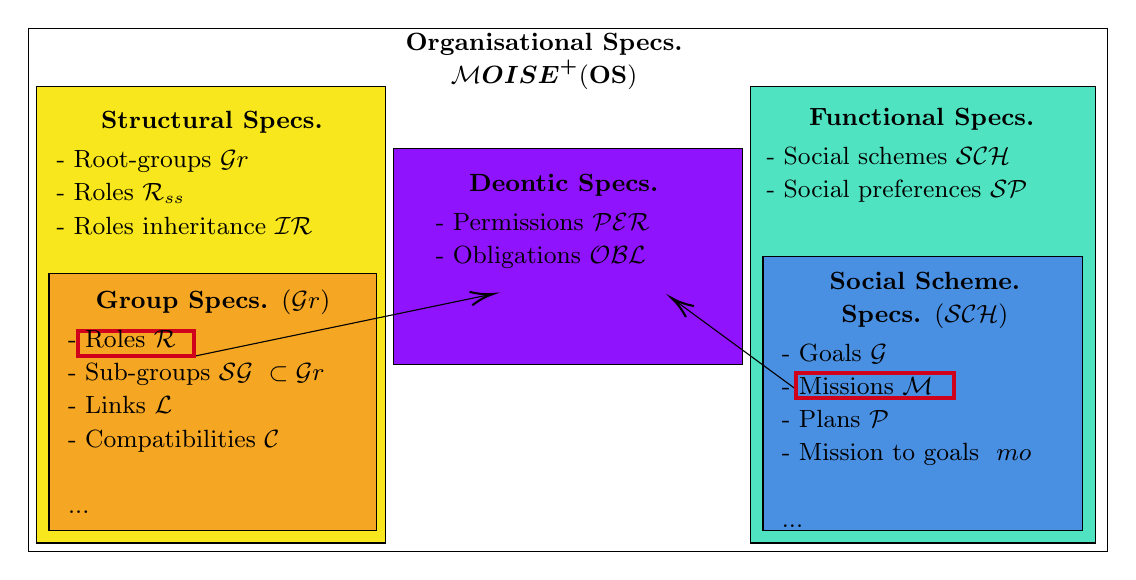
\begin{tikzpicture}[x=0.75pt,y=0.75pt,yscale=-1,xscale=1]
%uncomment if require: \path (0,1656); %set diagram left start at 0, and has height of 1656

%Shape: Rectangle [id:dp6756844921493015] 
\draw  [fill={rgb, 255:red, 248; green, 231; blue, 28 }  ,fill opacity=1 ] (46,1204) -- (214,1204) -- (214,1424) -- (46,1424) -- cycle ;
%Shape: Rectangle [id:dp3759944257810566] 
\draw  [fill={rgb, 255:red, 80; green, 227; blue, 194 }  ,fill opacity=1 ] (390,1204) -- (556,1204) -- (556,1424) -- (390,1424) -- cycle ;
%Shape: Rectangle [id:dp28244406216006945] 
\draw  [fill={rgb, 255:red, 144; green, 19; blue, 254 }  ,fill opacity=1 ] (218,1234) -- (386,1234) -- (386,1338) -- (218,1338) -- cycle ;
%Shape: Rectangle [id:dp32232123359581766] 
\draw   (42,1176) -- (562,1176) -- (562,1428) -- (42,1428) -- cycle ;
%Shape: Rectangle [id:dp7605706269262755] 
\draw  [fill={rgb, 255:red, 74; green, 144; blue, 226 }  ,fill opacity=1 ] (396,1286) -- (550,1286) -- (550,1418) -- (396,1418) -- cycle ;
%Shape: Rectangle [id:dp33110985390647496] 
\draw   (52,1294) -- (210,1294) -- (210,1418) -- (52,1418) -- cycle ;
%Shape: Rectangle [id:dp8653560038381976] 
\draw  [fill={rgb, 255:red, 245; green, 166; blue, 35 }  ,fill opacity=1 ] (52,1294) -- (210,1294) -- (210,1418) -- (52,1418) -- cycle ;
%Straight Lines [id:da09781093164567278] 
\draw    (412,1350) -- (353.61,1307.18) ;
\draw [shift={(352,1306)}, rotate = 36.25] [color={rgb, 255:red, 0; green, 0; blue, 0 }  ][line width=0.75]    (10.93,-3.29) .. controls (6.95,-1.4) and (3.31,-0.3) .. (0,0) .. controls (3.31,0.3) and (6.95,1.4) .. (10.93,3.29)   ;
%Straight Lines [id:da3938396723807833] 
\draw    (122,1334) -- (264.04,1304.41) ;
\draw [shift={(266,1304)}, rotate = 168.23] [color={rgb, 255:red, 0; green, 0; blue, 0 }  ][line width=0.75]    (10.93,-3.29) .. controls (6.95,-1.4) and (3.31,-0.3) .. (0,0) .. controls (3.31,0.3) and (6.95,1.4) .. (10.93,3.29)   ;
%Shape: Rectangle [id:dp269311335478327] 
\draw  [color={rgb, 255:red, 208; green, 2; blue, 27 }  ,draw opacity=1 ][line width=1.5]  (66,1322) -- (122,1322) -- (122,1334) -- (66,1334) -- cycle ;
%Shape: Rectangle [id:dp7449860119164387] 
\draw  [color={rgb, 255:red, 208; green, 2; blue, 27 }  ,draw opacity=1 ][line width=1.5]  (412,1342) -- (488,1342) -- (488,1354) -- (412,1354) -- cycle ;


% Text Node
\draw (472.5,1237.41) node   [align=left] {\begin{minipage}[lt]{112.2pt}\setlength\topsep{0pt}
\begin{center}
\textbf{{\small Functional Specs.}}
\end{center}
{\small  - Social schemes $\displaystyle \mathcal{SCH}$}\\{\small  - Social preferences $\displaystyle \mathcal{SP}$}
\end{minipage}};
% Text Node
\draw (474,1355) node   [align=left] {\begin{minipage}[lt]{103.36pt}\setlength\topsep{0pt}
\begin{center}
\textbf{{\small Social Scheme.}}\\{\small \textbf{Specs. }$\displaystyle (\mathcal{SCH})$}
\end{center}
{\small  - Goals $\displaystyle \mathcal{G}$}\\{\small  - Missions $\displaystyle \mathcal{M}$}\\{\small  - Plans $\displaystyle \mathcal{P}$}\\{\small  - Mission to goals \ $\displaystyle mo$}\\\\{\small  ...}
\end{minipage}};
% Text Node
\draw (131,1356) node   [align=left] {\begin{minipage}[lt]{104.72pt}\setlength\topsep{0pt}
\begin{center}
{\small \textbf{Group Specs. }$\displaystyle (\mathcal{G} r)$}
\end{center}
{\small  - Roles $\displaystyle \mathcal{R}$}\\{\small  - Sub-groups $\displaystyle \mathcal{SG} \ \subset \mathcal{G} r$}\\{\small  - Links $\displaystyle \mathcal{L}$}\\{\small  - Compatibilities $\displaystyle \mathcal{C}$}\\\\{\small  ...}
\end{minipage}};
% Text Node
\draw (181,1177) node [anchor=north west][inner sep=0.75pt]   [align=left] {\begin{minipage}[lt]{162.41pt}\setlength\topsep{0pt}
\begin{center}
{\small \textbf{Organisational Specs. }$\displaystyle \mathcal{M}\boldsymbol{OISE^{+}}$($\displaystyle \mathbf{OS}$)}
\end{center}

\end{minipage}};
% Text Node
\draw (300,1269.09) node   [align=left] {\begin{minipage}[lt]{92.48pt}\setlength\topsep{0pt}
\begin{center}
\textbf{{\small Deontic Specs.}}
\end{center}
{\small  - Permissions $\displaystyle \mathcal{PER}$}\\{\small  - Obligations $\displaystyle \mathcal{OBL}$}
\end{minipage}};
% Text Node
\draw (130.5,1245.69) node   [align=left] {\begin{minipage}[lt]{112.2pt}\setlength\topsep{0pt}
\begin{center}
\textbf{{\small Structural Specs.}}
\end{center}
{\small  - Root-groups $\displaystyle \mathcal{G} r$}\\{\small  - Roles $\displaystyle \mathcal{R}_{ss}$}\\{\small  - Roles inheritance $\displaystyle \mathcal{IR}$}
\end{minipage}};


\end{tikzpicture}
    \caption{\textbf{Une vue synthétique de} $\mathbfcal{M}\mathbf{OISE^+}$}
    \label{fig:moise_model}
\end{figure}

\noindent \textbf{Spécifications structurelles (SS):}
Elles définissent la structure des agents, notées
$
\mathcal{SS} = \langle \mathcal{R}, \mathcal{IR}, \mathcal{G} \rangle,
$
où \(\mathcal{R}\) est l'ensemble des rôles, avec une relation d'héritage \(\mathcal{IR}\) (c'est-à-dire, \(\rho_1 \sqsubset \rho_2\) si \(\rho_1\) hérite de \(\rho_2\)). De plus, \(\mathcal{GR}\) spécifie des groupes sous la forme 
$
\langle \mathcal{R}, \mathcal{SG}, \mathcal{L}^{intra}, \mathcal{L}^{inter}, \mathcal{C}^{intra}, \mathcal{C}^{inter}, np, ng \rangle,
$
où \(\mathcal{L}\) désigne les liens (connaissance, communication, autorité) et \(\mathcal{C}\) les compatibilités entre rôles, avec \(np\) et \(ng\) indiquant respectivement le nombre de rôles et de sous-groupes.

\vspace{0.5em}
\noindent \textbf{Spécifications fonctionnelles (FS):}
Elles décrivent les objectifs des agents et sont notées
$
\mathcal{FS} = \langle \mathcal{SCH}, \mathcal{PO} \rangle.
$
Le schéma social \(\mathcal{SCH}\) comprend les objectifs globaux \(\mathcal{G}\), les missions \(\mathcal{M}\) et les plans \(\mathcal{P}\) organisant ces objectifs (via l'opérateur \(op\) pour séquence, choix ou parallèle). Les missions regroupent des ensembles d'objectifs (\(mo\)) et le nombre d'agents par mission est donné par \(nm\), tandis que \(\mathcal{PO}\) représente les préférences (ex. \(m_1 \prec m_2\)).

\vspace{0.5em}
\noindent \textbf{Spécifications déontiques (DS):}
Elles précisent la relation entre rôles et objectifs, notées
$
\mathcal{DS} = \langle \mathcal{OBL}, \mathcal{PER} \rangle.
$
Les contraintes temporelles \(\mathcal{TC}\) fixent les périodes pour les permissions/obligations (ex. \(Any\) pour tout moment). Les obligations \(\mathcal{OBL}\) imposent aux agents en rôle \(\rho_a\) d'exécuter la mission \(m\) aux moments \(tc\), tandis que les permissions \(\mathcal{PER}\) les autorisent. La fonction \(rds\) associe à chaque rôle une spécification sous la forme 
$
\langle tc, y, m \rangle,
$
avec \(y=0\) pour permission et \(y=1\) pour obligation.


Les autres spécifications structurelles (compatibilités, liens) sont inhérentes aux rôles. De même, les objectifs (incluant missions et \(mo\)) sont inhérents aux autres spécifications fonctionnelles (plans, cardinalités, ordres de préférence). Considérer les rôles, les missions et les permissions/obligations est suffisant pour lier \(\mathcal{M}OISE^+\) au Dec-POMDP.

\begin{figure*}[t]

    \label{eq:single_value_function}
    \raggedright
    \textbf{\textit{Définition 1} \quad Fonction de valeur d'état adaptée aux \textbf{Guide de Contrainte} en mode AEC :}

    \begin{scriptsize}
      \vspace{-0.3cm}
      \begin{gather*}
      V^{\pi^j}(s_t) = \hspace{-0.75cm} \sum_{\textcolor{red}{ \substack{a_{t} \in A \text{ si } rn() < ch_{t}, \\ 
      a_{t} \in A_{t} \text{ sinon}}
      }}{\hspace{-0.7cm} \pi_i(a_{t} | \omega_t)} \sum_{s_{t+1} \in S}{\hspace{-0.1cm} T(s_{t+1} | s_t, a_{t})\Bigl[R(s_t,a_{t},s_{t+1}) + \hspace{-0.1cm} \textcolor{blue}{ \sum_{m \in \mathcal{M}_i}{ \hspace{-0.1cm} v_m(t) \frac{grg_m(h_{t+1})}{1 - p + \epsilon} } } + \textcolor{red}{(1-ch_t) \times rrg(\omega_t,a_{t+1})} + V^{\pi^j_{i+1 \ mod \ n}}(s_{t+1})\Bigr]}
    \end{gather*}  
    %
    \vspace{-0.3cm}
    %
    \textcolor{red}{$\hspace{0cm}\text{Avec } rag(h_t, \omega_t) = A_{t} \times \mathbb{R} \text{, } \langle a_t, ch_{t} \rangle \in A_{t} \times \mathbb{R} \text{ ; et } rn: \emptyset \to [0,1[ \text{, une fonction aléatoire uniforme}$}
    %
    \vspace{-0cm}
    \textcolor{blue}{
    \begin{gather*}
    \hspace{-4.1cm}\text{Avec } \omega_t = O(\omega_t | s_t, a_t) \text{ ; } h_t = \{h_0 = \langle \rangle, h_{t+1} = \langle h_t, \langle \omega_{t+1}, a_{t+1} \rangle \rangle \} \text{ ; } grg_m(h) = \hspace{-0.8cm} \sum_{(grg_i,w_i) \in mo(m)}{\hspace{-0.8cm} w_i \times grg_i(h)} \text{ ; } \epsilon \in \mathbb{R}_{>0} \text{ ; }
    \end{gather*}
    }
    \vspace{-1.05cm}
    \textcolor{blue}{
    \begin{gather*}
    \hspace{-8.5cm}
    v_m(t) = \{ 1 \text{ si } t \in t_c \text{ ; sinon } 0 \} \text{ ; et } \mathcal{M}_i = \{m_j \mid \langle ar(i),m_j,t_c,p \rangle \in \mathcal{M}\}
    \end{gather*}
    }
    \vspace{-0.6cm}

    \end{scriptsize}

\end{figure*}

\subsection{Liaison de \(\mathcal{M}OISE^+\) avec le MARL}

\begin{figure}[h!]

    \adjustbox{lap=-0.38cm}{\tikzset{every picture/.style={line width=0.75pt}} %set default line width to 0.75pt        

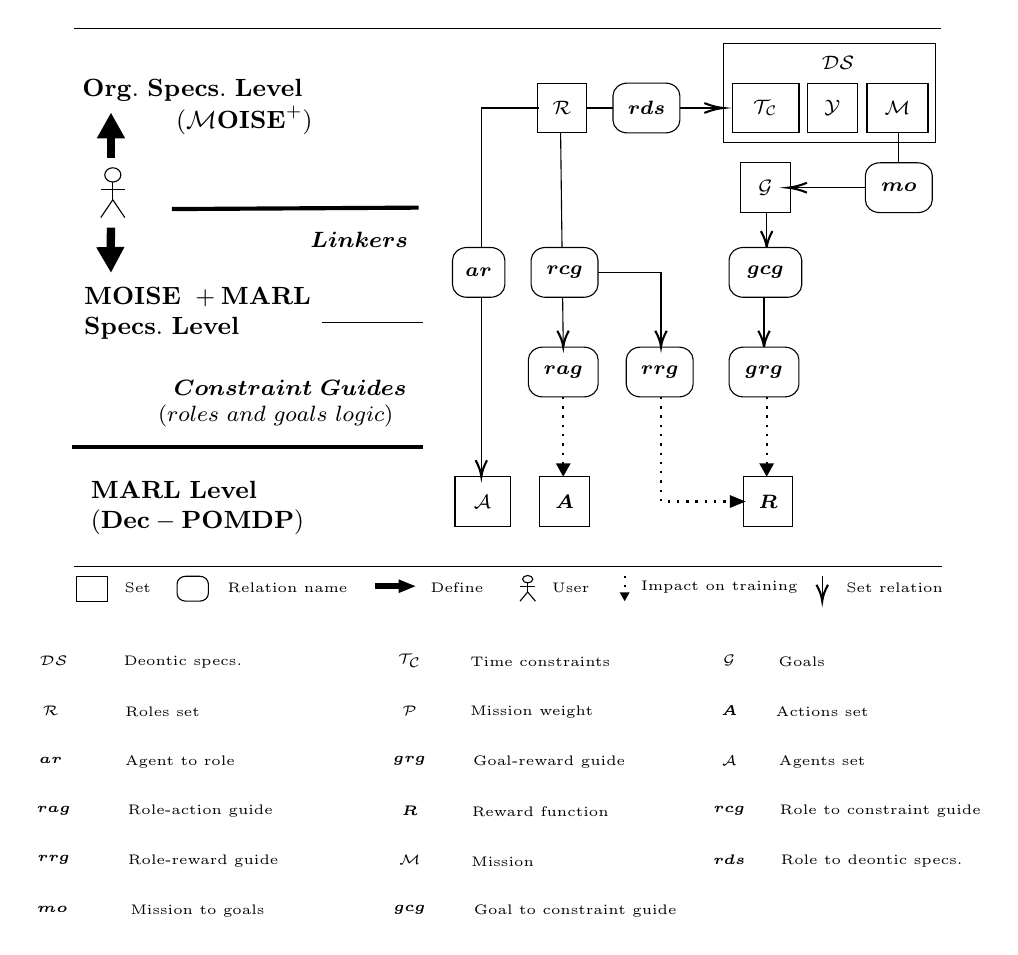
\begin{tikzpicture}[x=0.75pt,y=0.75pt,yscale=-1.2,xscale=1.4]
    %uncomment if require: \path (0,2584); %set diagram left start at 0, and has height of 2584

    %Straight Lines [id:da4973066741986565] 
    \draw [line width=1.5]    (118.21,2302.58) -- (203.1,2302) ;
    %Straight Lines [id:da14807114776731778] 
    \draw    (368.35,2272) -- (368.35,2294) -- (332.16,2294) ;
    \draw [shift={(330.16,2294)}, rotate = 360] [color={rgb, 255:red, 0; green, 0; blue, 0 }  ][line width=0.75]    (6.56,-1.97) .. controls (4.17,-0.84) and (1.99,-0.18) .. (0,0) .. controls (1.99,0.18) and (4.17,0.84) .. (6.56,1.97)   ;
    %Straight Lines [id:da16285043353898754] 
    \draw [line width=1.5]    (83.88,2398) -- (204.61,2398) ;
    %Straight Lines [id:da6299512000169913] 
    \draw    (169.94,2348) -- (204.61,2348) ;
    %Straight Lines [id:da64750232417664] 
    \draw    (84.65,2446) -- (383.15,2446) ;
    %Straight Lines [id:da35895220906699743] 
    \draw    (84.65,2230) -- (383,2230) ;
    %Straight Lines [id:da715014372569708] 
    \draw    (244.68,2262) -- (224.68,2262) -- (224.68,2408) ;
    \draw [shift={(224.68,2410)}, rotate = 270] [color={rgb, 255:red, 0; green, 0; blue, 0 }  ][line width=0.75]    (6.56,-1.97) .. controls (4.17,-0.84) and (1.99,-0.18) .. (0,0) .. controls (1.99,0.18) and (4.17,0.84) .. (6.56,1.97)   ;
    %Straight Lines [id:da71870438525014] 
    \draw    (251.96,2328) -- (286.51,2328) -- (286.51,2356) ;
    \draw [shift={(286.51,2358)}, rotate = 270] [color={rgb, 255:red, 0; green, 0; blue, 0 }  ][line width=0.75]    (6.56,-1.97) .. controls (4.17,-0.84) and (1.99,-0.18) .. (0,0) .. controls (1.99,0.18) and (4.17,0.84) .. (6.56,1.97)   ;
    %Straight Lines [id:da6006267784187092] 
    \draw [line width=0.75]  [dash pattern={on 0.84pt off 2.51pt}]  (252.87,2378) -- (252.87,2407) ;
    \draw [shift={(252.87,2410)}, rotate = 270] [fill={rgb, 255:red, 0; green, 0; blue, 0 }  ][line width=0.08]  [draw opacity=0] (5.36,-2.57) -- (0,0) -- (5.36,2.57) -- cycle    ;
    %Straight Lines [id:da8743336135156266] 
    \draw    (322.88,2304) -- (322.88,2316) ;
    \draw [shift={(322.88,2318)}, rotate = 270] [color={rgb, 255:red, 0; green, 0; blue, 0 }  ][line width=0.75]    (6.56,-1.97) .. controls (4.17,-0.84) and (1.99,-0.18) .. (0,0) .. controls (1.99,0.18) and (4.17,0.84) .. (6.56,1.97)   ;
    %Straight Lines [id:da14641229967966152] 
    \draw [line width=0.75]  [dash pattern={on 0.84pt off 2.51pt}]  (322.88,2378) -- (322.88,2407) ;
    \draw [shift={(322.88,2410)}, rotate = 270] [fill={rgb, 255:red, 0; green, 0; blue, 0 }  ][line width=0.08]  [draw opacity=0] (5.36,-2.57) -- (0,0) -- (5.36,2.57) -- cycle    ;
    %Straight Lines [id:da9260929933425808] 
    \draw [line width=0.75]  [dash pattern={on 0.84pt off 2.51pt}]  (286.51,2378) -- (286.51,2420) -- (312.61,2420) ;
    \draw [shift={(315.61,2420)}, rotate = 180] [fill={rgb, 255:red, 0; green, 0; blue, 0 }  ][line width=0.08]  [draw opacity=0] (5.36,-2.57) -- (0,0) -- (5.36,2.57) -- cycle    ;
    %Straight Lines [id:da3057006030233673] 
    \draw [line width=0.75]  [dash pattern={on 0.84pt off 2.51pt}]  (274,2449.7) -- (274,2457) ;
    \draw [shift={(274,2460)}, rotate = 270] [fill={rgb, 255:red, 0; green, 0; blue, 0 }  ][line width=0.08]  [draw opacity=0] (3.57,-1.72) -- (0,0) -- (3.57,1.72) -- cycle    ;
    %Straight Lines [id:da07288166228322246] 
    \draw    (342,2449.98) -- (342,2458) ;
    \draw [shift={(342,2460)}, rotate = 270] [color={rgb, 255:red, 0; green, 0; blue, 0 }  ][line width=0.75]    (6.56,-1.97) .. controls (4.17,-0.84) and (1.99,-0.18) .. (0,0) .. controls (1.99,0.18) and (4.17,0.84) .. (6.56,1.97)   ;
    %Shape: Ellipse [id:dp8508274348425935] 
    \draw   (95.09,2288.86) .. controls (95.09,2287.28) and (96.33,2286) .. (97.85,2286) .. controls (99.38,2286) and (100.62,2287.28) .. (100.62,2288.86) .. controls (100.62,2290.44) and (99.38,2291.71) .. (97.85,2291.71) .. controls (96.33,2291.71) and (95.09,2290.44) .. (95.09,2288.86) -- cycle ;
    %Straight Lines [id:da3825450168053828] 
    \draw    (97.85,2291.71) -- (97.85,2298.86) ;
    %Straight Lines [id:da521321206042058] 
    \draw    (97.85,2298.86) -- (93.71,2306) ;
    %Straight Lines [id:da055514206493922025] 
    \draw    (97.85,2298.86) -- (102,2306) ;
    %Straight Lines [id:da8996496708356774] 
    \draw    (102,2294.57) -- (93.71,2294.57) ;

    %Straight Lines [id:da31678488015771755] 
    \draw [line width=2.25]    (188,2454) -- (196.97,2454) ;
    \draw [shift={(201.97,2454)}, rotate = 180] [fill={rgb, 255:red, 0; green, 0; blue, 0 }  ][line width=0.08]  [draw opacity=0] (5.72,-2.75) -- (0,0) -- (5.72,2.75) -- cycle    ;
    %Shape: Ellipse [id:dp3927356466672782] 
    \draw   (238.88,2451.17) .. controls (238.88,2450.36) and (239.67,2449.7) .. (240.64,2449.7) .. controls (241.61,2449.7) and (242.4,2450.36) .. (242.4,2451.17) .. controls (242.4,2451.99) and (241.61,2452.65) .. (240.64,2452.65) .. controls (239.67,2452.65) and (238.88,2451.99) .. (238.88,2451.17) -- cycle ;
    %Straight Lines [id:da3365602555559104] 
    \draw    (240.64,2452.65) -- (240.64,2456.32) ;
    %Straight Lines [id:da7990875235744026] 
    \draw    (240.64,2456.32) -- (238,2460) ;
    %Straight Lines [id:da23945649338821617] 
    \draw    (240.64,2456.32) -- (243.28,2460) ;
    %Straight Lines [id:da11927353559661591] 
    \draw    (243.28,2454.12) -- (238,2454.12) ;

    %Straight Lines [id:da5816423191130675] 
    \draw    (251.96,2272) -- (252.85,2356) ;
    \draw [shift={(252.87,2358)}, rotate = 269.39] [color={rgb, 255:red, 0; green, 0; blue, 0 }  ][line width=0.75]    (6.56,-1.97) .. controls (4.17,-0.84) and (1.99,-0.18) .. (0,0) .. controls (1.99,0.18) and (4.17,0.84) .. (6.56,1.97)   ;
    %Straight Lines [id:da9310455126832857] 
    \draw    (321.97,2338) -- (321.97,2356) ;
    \draw [shift={(321.97,2358)}, rotate = 270] [color={rgb, 255:red, 0; green, 0; blue, 0 }  ][line width=0.75]    (6.56,-1.97) .. controls (4.17,-0.84) and (1.99,-0.18) .. (0,0) .. controls (1.99,0.18) and (4.17,0.84) .. (6.56,1.97)   ;
    %Shape: Rectangle [id:dp293492578719597] 
    \draw   (120,2453) .. controls (120,2451.34) and (121.34,2450) .. (123,2450) -- (127.72,2450) .. controls (129.37,2450) and (130.72,2451.34) .. (130.72,2453) -- (130.72,2457) .. controls (130.72,2458.66) and (129.37,2460) .. (127.72,2460) -- (123,2460) .. controls (121.34,2460) and (120,2458.66) .. (120,2457) -- cycle ;
    %Straight Lines [id:da33566712615128225] 
    \draw    (261.05,2262) -- (306,2262) ;
    \draw [shift={(308,2262)}, rotate = 180] [color={rgb, 255:red, 0; green, 0; blue, 0 }  ][line width=0.75]    (6.56,-1.97) .. controls (4.17,-0.84) and (1.99,-0.18) .. (0,0) .. controls (1.99,0.18) and (4.17,0.84) .. (6.56,1.97)   ;
    %Shape: Rectangle [id:dp28383270948937667] 
    \draw   (308,2236) -- (381.08,2236) -- (381.08,2276) -- (308,2276) -- cycle ;
    %Straight Lines [id:da18020989903965012] 
    \draw [line width=3]    (97.22,2282) -- (97.22,2270) ;
    \draw [shift={(97.22,2264)}, rotate = 90] [fill={rgb, 255:red, 0; green, 0; blue, 0 }  ][line width=0.08]  [draw opacity=0] (10.18,-4.89) -- (0,0) -- (10.18,4.89) -- cycle    ;
    %Straight Lines [id:da018421338049046554] 
    \draw [line width=3]    (97.22,2310) -- (97.11,2322.37) ;
    \draw [shift={(97.22,2328)}, rotate = 268.86] [fill={rgb, 255:red, 0; green, 0; blue, 0 }  ][line width=0.08]  [draw opacity=0] (10.18,-4.89) -- (0,0) -- (10.18,4.89) -- cycle    ;
    %Shape: Rectangle [id:dp7281037051878541] 
    \draw   (85.42,2450) -- (96.13,2450) -- (96.13,2460) -- (85.42,2460) -- cycle ;

    % Text Node
    \draw (362,2544.5) node  [font=\tiny] [align=left] {Role to constraint guide};
    % Text Node
    \draw (342,2524.5) node  [font=\tiny] [align=left] {Agents set};
    % Text Node
    \draw (342,2504.5) node  [font=\tiny] [align=left] {Actions set};
    % Text Node
    \draw (257,2584.5) node  [font=\tiny] [align=left] {Goal to constraint guide};
    % Text Node
    \draw (335,2484.5) node  [font=\tiny] [align=left] {Goals};
    % Text Node
    \draw (359,2564.5) node  [font=\tiny] [align=left] {Role to deontic specs.};
    % Text Node
    \draw (232,2564.5) node  [font=\tiny] [align=left] {Mission};
    % Text Node
    \draw (245,2544.5) node  [font=\tiny] [align=left] {Reward function};
    % Text Node
    \draw (248,2524.5) node  [font=\tiny] [align=left] {Goal-reward guide};
    % Text Node
    \draw (242,2504.5) node  [font=\tiny] [align=left] {Mission weight};
    % Text Node
    \draw (245,2484.5) node  [font=\tiny] [align=left] {Time constraints};
    % Text Node
    \draw (127,2584.5) node  [font=\tiny] [align=left] {Mission to goals};
    % Text Node
    \draw (129,2564.5) node  [font=\tiny] [align=left] {Role-reward guide};
    % Text Node
    \draw (128,2544.5) node  [font=\tiny] [align=left] {Role-action guide};
    % Text Node
    \draw (121,2524.5) node  [font=\tiny] [align=left] {Agent to role};
    % Text Node
    \draw (115,2504.5) node  [font=\tiny] [align=left] {Roles set};
    % Text Node
    \draw (122,2484.5) node  [font=\tiny] [align=left] {Deontic specs.};
    % Text Node
    \draw (310,2544) node  [font=\tiny] [align=left] {$\displaystyle \boldsymbol{rcg}$};
    % Text Node
    \draw (200,2504) node  [font=\tiny] [align=left] {$\displaystyle \mathcal{P}$};
    % Text Node
    \draw (200,2484) node  [font=\tiny] [align=left] {$\displaystyle \mathcal{T_{C}}$};
    % Text Node
    \draw (200,2564) node  [font=\tiny] [align=left] {$\displaystyle \mathcal{M}$};
    % Text Node
    \draw (77.5,2484) node  [font=\tiny] [align=left] {$\displaystyle \mathcal{DS}$};
    % Text Node
    \draw (310,2564) node  [font=\tiny] [align=left] {$\displaystyle \boldsymbol{rds}$};
    % Text Node
    \draw (310,2504) node  [font=\tiny] [align=left] {$\displaystyle \boldsymbol{A}$};
    % Text Node
    \draw (200,2544) node  [font=\tiny] [align=left] {$\displaystyle \boldsymbol{R}$};
    % Text Node
    \draw (310,2524) node  [font=\tiny] [align=left] {$\displaystyle \mathcal{A}$};
    % Text Node
    \draw (200,2524) node  [font=\tiny] [align=left] {$\displaystyle \boldsymbol{grg}$};
    % Text Node
    \draw (77.5,2564) node  [font=\tiny] [align=left] {$\displaystyle \boldsymbol{rrg}$};
    % Text Node
    \draw (77.5,2544) node  [font=\tiny] [align=left] {$\displaystyle \boldsymbol{rag}$};
    % Text Node
    \draw (200,2584) node  [font=\tiny] [align=left] {$\displaystyle \boldsymbol{gcg}$};
    % Text Node
    \draw (76.5,2524) node  [font=\tiny] [align=left] {$\displaystyle \boldsymbol{ar}$};
    % Text Node
    \draw (77,2584) node  [font=\tiny] [align=left] {$\displaystyle \boldsymbol{mo}$};
    % Text Node
    \draw (76.5,2504) node  [font=\tiny] [align=left] {$\displaystyle \mathcal{R}$};
    % Text Node
    \draw (310,2484) node  [font=\tiny] [align=left] {$\displaystyle \mathcal{G}$};


    % Text Node
    \draw  [fill={rgb, 255:red, 255; green, 255; blue, 255 }  ,fill opacity=1 ]  (241.82,2323) .. controls (241.82,2320.24) and (244.06,2318) .. (246.82,2318) -- (259.82,2318) .. controls (262.58,2318) and (264.82,2320.24) .. (264.82,2323) -- (264.82,2333) .. controls (264.82,2335.76) and (262.58,2338) .. (259.82,2338) -- (246.82,2338) .. controls (244.06,2338) and (241.82,2335.76) .. (241.82,2333) -- cycle  ;
    \draw (253.32,2328) node  [font=\scriptsize] [align=left] {$\displaystyle \boldsymbol{rcg}$};
    % Text Node
    \draw    (337,2252) -- (354,2252) -- (354,2272) -- (337,2272) -- cycle  ;
    \draw (345.5,2262) node  [font=\scriptsize] [align=left] {$\displaystyle \mathcal{Y}$};
    % Text Node
    \draw    (311,2252) -- (334,2252) -- (334,2272) -- (311,2272) -- cycle  ;
    \draw (322.5,2262) node  [font=\scriptsize] [align=left] {$\displaystyle \mathcal{T_{C}}$};
    % Text Node
    \draw    (357.39,2252) -- (378.39,2252) -- (378.39,2272) -- (357.39,2272) -- cycle  ;
    \draw (367.89,2262) node  [font=\scriptsize] [align=left] {$\displaystyle \mathcal{M}$};
    % Text Node
    \draw (347.43,2244) node  [font=\scriptsize] [align=left] {$\displaystyle \mathcal{DS}$};
    % Text Node
    \draw  [fill={rgb, 255:red, 255; green, 255; blue, 255 }  ,fill opacity=1 ]  (270,2257) .. controls (270,2254.24) and (272.24,2252) .. (275,2252) -- (288,2252) .. controls (290.76,2252) and (293,2254.24) .. (293,2257) -- (293,2267) .. controls (293,2269.76) and (290.76,2272) .. (288,2272) -- (275,2272) .. controls (272.24,2272) and (270,2269.76) .. (270,2267) -- cycle  ;
    \draw (281.5,2262) node  [font=\scriptsize] [align=left] {$\displaystyle \boldsymbol{rds}$};
    % Text Node
    \draw (158,2454.5) node  [font=\tiny] [align=left] {Relation name};
    % Text Node
    \draw (106.46,2454.5) node  [font=\tiny] [align=left] {Set};
    % Text Node
    \draw (255.47,2454.5) node  [font=\tiny] [align=left] {User};
    % Text Node
    \draw (216.32,2454.5) node  [font=\tiny] [align=left] {Define};
    % Text Node
    \draw (366.91,2454.5) node  [font=\tiny] [align=left] {Set relation};
    % Text Node
    \draw (306.61,2454.5) node  [font=\tiny] [align=left] {Impact on training};
    % Text Node
    \draw    (244.82,2410) -- (261.82,2410) -- (261.82,2430) -- (244.82,2430) -- cycle  ;
    \draw (253.32,2420) node  [font=\scriptsize] [align=left] {$\displaystyle \boldsymbol{A}$};
    % Text Node
    \draw    (314.84,2410) -- (331.84,2410) -- (331.84,2430) -- (314.84,2430) -- cycle  ;
    \draw (323.34,2420) node  [font=\scriptsize] [align=left] {$\displaystyle \boldsymbol{R}$};
    % Text Node
    \draw    (215.63,2410) -- (234.63,2410) -- (234.63,2430) -- (215.63,2430) -- cycle  ;
    \draw (225.13,2420) node  [font=\scriptsize] [align=left] {$\displaystyle \mathcal{A}$};
    % Text Node
    \draw  [fill={rgb, 255:red, 255; green, 255; blue, 255 }  ,fill opacity=1 ]  (309.97,2363) .. controls (309.97,2360.24) and (312.21,2358) .. (314.97,2358) -- (328.97,2358) .. controls (331.73,2358) and (333.97,2360.24) .. (333.97,2363) -- (333.97,2373) .. controls (333.97,2375.76) and (331.73,2378) .. (328.97,2378) -- (314.97,2378) .. controls (312.21,2378) and (309.97,2375.76) .. (309.97,2373) -- cycle  ;
    \draw (321.97,2368) node  [font=\scriptsize] [align=left] {$\displaystyle \boldsymbol{grg}$};
    % Text Node
    \draw    (274.56,2363) .. controls (274.56,2360.24) and (276.8,2358) .. (279.56,2358) -- (292.56,2358) .. controls (295.32,2358) and (297.56,2360.24) .. (297.56,2363) -- (297.56,2373) .. controls (297.56,2375.76) and (295.32,2378) .. (292.56,2378) -- (279.56,2378) .. controls (276.8,2378) and (274.56,2375.76) .. (274.56,2373) -- cycle  ;
    \draw (286.06,2368) node  [font=\scriptsize] [align=left] {$\displaystyle \boldsymbol{rrg}$};
    % Text Node
    \draw    (240.87,2363) .. controls (240.87,2360.24) and (243.11,2358) .. (245.87,2358) -- (259.87,2358) .. controls (262.63,2358) and (264.87,2360.24) .. (264.87,2363) -- (264.87,2373) .. controls (264.87,2375.76) and (262.63,2378) .. (259.87,2378) -- (245.87,2378) .. controls (243.11,2378) and (240.87,2375.76) .. (240.87,2373) -- cycle  ;
    \draw (252.87,2368) node  [font=\scriptsize] [align=left] {$\displaystyle \boldsymbol{rag}$};
    % Text Node
    \draw (156.15,2380.5) node  [font=\footnotesize] [align=left] {$\displaystyle  \begin{array}{{>{\displaystyle}l}}
                \ \ \boldsymbol{Constraint\ Guides} \\
                ( roles\ and\ goals\ logic)
            \end{array}$};
    % Text Node
    \draw  [fill={rgb, 255:red, 255; green, 255; blue, 255 }  ,fill opacity=1 ]  (309.93,2323) .. controls (309.93,2320.24) and (312.17,2318) .. (314.93,2318) -- (329.93,2318) .. controls (332.69,2318) and (334.93,2320.24) .. (334.93,2323) -- (334.93,2333) .. controls (334.93,2335.76) and (332.69,2338) .. (329.93,2338) -- (314.93,2338) .. controls (312.17,2338) and (309.93,2335.76) .. (309.93,2333) -- cycle  ;
    \draw (322.43,2328) node  [font=\scriptsize] [align=left] {$\displaystyle \boldsymbol{gcg}$};
    % Text Node
    \draw  [fill={rgb, 255:red, 255; green, 255; blue, 255 }  ,fill opacity=1 ]  (214.77,2323) .. controls (214.77,2320.24) and (217.01,2318) .. (219.77,2318) -- (227.77,2318) .. controls (230.53,2318) and (232.77,2320.24) .. (232.77,2323) -- (232.77,2333) .. controls (232.77,2335.76) and (230.53,2338) .. (227.77,2338) -- (219.77,2338) .. controls (217.01,2338) and (214.77,2335.76) .. (214.77,2333) -- cycle  ;
    \draw (223.77,2328) node  [font=\scriptsize] [align=left] {$\displaystyle \boldsymbol{ar}$};
    % Text Node
    \draw  [fill={rgb, 255:red, 255; green, 255; blue, 255 }  ,fill opacity=1 ]  (356.85,2289) .. controls (356.85,2286.24) and (359.08,2284) .. (361.85,2284) -- (374.85,2284) .. controls (377.61,2284) and (379.85,2286.24) .. (379.85,2289) -- (379.85,2299) .. controls (379.85,2301.76) and (377.61,2304) .. (374.85,2304) -- (361.85,2304) .. controls (359.08,2304) and (356.85,2301.76) .. (356.85,2299) -- cycle  ;
    \draw (368.35,2294) node  [font=\scriptsize] [align=left] {$\displaystyle \boldsymbol{mo}$};
    % Text Node
    \draw (127,2344.5) node  [font=\small] [align=left] {$\displaystyle  \begin{array}{{>{\displaystyle}l}}
                \mathbf{MOISE\ +MARL} \\
                \mathbf{Specs.\ Level}
            \end{array}$};
    % Text Node
    \draw (127,2422.5) node  [font=\small] [align=left] {$\displaystyle  \begin{array}{{>{\displaystyle}l}}
                \mathbf{MARL\ Level} \\
                \mathbf{(Dec-POMDP)}
            \end{array}$};
    % Text Node
    \draw    (243.91,2252) -- (260.91,2252) -- (260.91,2272) -- (243.91,2272) -- cycle  ;
    \draw (252.41,2262) node  [font=\scriptsize] [align=left] {$\displaystyle \mathcal{R}$};
    % Text Node
    \draw (182.64,2315) node  [font=\footnotesize] [align=left] {$\displaystyle \boldsymbol{Linkers}$};
    % Text Node
    \draw    (313.93,2284) -- (330.93,2284) -- (330.93,2304) -- (313.93,2304) -- cycle  ;
    \draw (322.43,2294) node  [font=\scriptsize] [align=left] {$\displaystyle \mathcal{G}$};
    % Text Node
    \draw (127,2261.5) node  [font=\small] [align=left] {$\displaystyle  \begin{array}{{>{\displaystyle}l}}
                \mathbf{{\displaystyle Org.\ Specs.\ Level}} \\
                {\displaystyle \ \ \ \ \ \ \ \ \ \ \ (\mathcal{M}\mathbf{OISE^+})}
            \end{array}$};


\end{tikzpicture}}
    \caption{\textbf{Une vue minimale du cadre MOISE+MARL} :
    Les utilisateurs définissent d'abord les spécifications de \(\mathcal{M}OISE^+\), qui incluent des rôles (\(\mathcal{R}\)) et des missions (\(\mathcal{M}\)) associées via \(rds\). Ensuite, ils créent des spécifications MOISE+MARL en définissant d'abord des \textbf{Guide de Contraintes} tels que \(rag\) et \(rrg\) pour spécifier la logique des rôles, et \(grg\) pour la logique des objectifs.
    Ensuite, des \textbf{Lieurs} sont utilisés pour connecter les agents aux rôles via \(ar\) et pour relier la logique des \textbf{Guide de Contrainte} aux spécifications définies de \(\mathcal{M}OISE^+\). Une fois cette configuration réalisée, des rôles peuvent être attribués aux agents, et le cadre MARL s'adapte en conséquence pendant l'entraînement.
    }
    \label{fig:mm_synthesis}
\end{figure}

Alors qu'\textit{AGR}~\cite{ferber2003} (Agent Group Role) est un cadre informel qui introduit des rôles par groupes, \(\mathcal{M}OISE^+\) offre une description plus détaillée et flexible des structures et fonctions d'un système multi-agent (MAS), facilitant ainsi la formalisation des politiques en MARL.

\medskip
\noindent \textbf{Guides de Contraintes} : Trois relations décrivent la logique des rôles et objectifs dans le cadre Dec-POMDP :
i) \textbf{Guide d'action de rôle} \(rag: H \times \Omega \to \mathcal{P}(A \times \mathbb{R})\) : Pour chaque couple \((h,\omega)\) (\(h\in H\), \(\omega\in \Omega\)), il associe un ensemble d'actions \(A_\omega \subseteq A\) avec une rigidité \(ch \in [0,1]\) (par défaut \(ch=1\)), restreignant ainsi le choix de la prochaine action ; \quad
ii) \textbf{Guide de récompense de rôle} \(rrg: H \times \Omega \times A \to \mathbb{R}\) : Défini par \(rrg(h,\omega,a)=r_m\) si \(a \notin A_\omega\) (avec \(rag(h,\omega)=A_\omega \times \mathbb{R}\)), et 0 sinon, afin d'encourager le respect du rôle ; \quad
iii) \textbf{Guide de récompense d'objectif} \(grg: H \to \mathbb{R}\) : Attribue un bonus \(r_b\) à la récompense globale si \(h\) contient une sous-séquence caractéristique \(h_g \in H_g\) correspondant à un objectif.

\medskip
\noindent \textbf{Lieurs} : Relient les spécifications de \(\mathcal{M}OISE^+\) aux Guides de Contraintes et aux agents :
i) \textbf{Agent vers Rôle} \(ar: \mathcal{A} \to \mathcal{R}\) (relation bijective) ; \quad
ii) \textbf{Rôle vers Guide de Contrainte} \(rcg: \mathcal{R} \to rag \cup rrg\) : Associe à chaque rôle une relation \(rag\) ou \(rrg\) ; \quad
iii) \textbf{Objectif vers Guide de Contrainte} \(gcg: \mathcal{G} \to grg\) : Relie chaque objectif à son guide \(grg\).

\textbf{La résolution du problème MOISE+MARL} consiste à trouver une politique conjointe 
$
\pi^j = \{\pi^j_0, \pi^j_1, \dots, \pi^j_n\}
$
maximisant la fonction de valeur d'état \(V^{\pi^j}\) (ou atteignant un seuil minimal), qui représente la récompense cumulative attendue à partir d'un état initial \(s \in S\) en suivant les actions conjointes \(a^j \in A^n\) sous l'effet de \textbf{Guides de Contraintes}. Cette fonction est définie pour des agents agissant de manière séquentielle et cyclique (mode AEC) (voir la \hyperref[eq:single_value_function]{Définition 1}). La \autoref{fig:mm_synthesis} illustre les liens entre \(\mathcal{M}OISE^+\) et le Dec-POMDP via MOISE+MARL.

À chaque instant \(t \in \mathbb{N}\) (initialement \(t=0\)), l'agent \(i = t \mod n\) doit assumer le rôle \(\rho_i = ar(i)\). Pour chaque spécification déontique valide 
$
d_i = rds(\rho_i) = \langle tc_i, y_i, m_i \rangle,
$
l'agent est autorisé (si \(y_i=0\)) ou obligé (si \(y_i=1\)) d'exécuter la mission \(m_i \in \mathcal{M}\) (avec \(\mathcal{G}_{m_i} = mo(m_i)\)). L'agent choisit d'abord une action parmi celles attendues \(A_t\) si une valeur aléatoire est inférieure à la rigidité \(ch_t\), sinon parmi l'ensemble \(A\); ainsi, un \(ch_t = 1\) impose une contrainte forte.

L'action appliquée à \(s_t\) conduit à l'état suivant \(s_{t+1}\), génère la prochaine observation \(\omega_{t+1}\) et une récompense. Celle-ci est la somme de la récompense globale et des ajustements organisationnels : 
i) un bonus (via les Guides de Récompense d'Objectif), pondéré par \(\frac{1}{1-p+\epsilon}\) pour ajuster son impact, et
ii) une pénalité (via les Guides de Récompense de Rôle), pondérée par la rigidité \(ch_t\) pour ajuster son impact.
Le calcul de la récompense cumulative se poursuit dans \(s_{t+1}\) avec l'agent suivant \((i+1) \mod n\).

\subsection{Faciliter l'implémentation des \textbf{Guide de Contrainte}}

Puisque les rôles, objectifs et missions sont de simples étiquettes, leur définition est implicite. Cependant, implémenter une relation \(rag\), \(rrg\) ou \(grg\) nécessite de définir de nombreux historiques, souvent redondants, rendant une définition extensionnelle fastidieuse. De plus, la logique de chaque \textbf{Guide de Contrainte} analyse la trajectoire de l'agent pour vérifier son appartenance à un ensemble prédéfini. Par exemple, \(rag\) détermine les actions attendues selon l'appartenance de la trajectoire à un ensemble donné et la nouvelle observation.

Une approche consiste à laisser l'utilisateur définir ses \textbf{Guides de Contrainte} via une logique personnalisée (par script, par exemple). Dans ce cas, la relation \(b_g: H \to \{0,1\}\) formalise la décision d'appartenance d'un historique à un ensemble \(H_g\).
Pour simplifier l'implémentation, nous proposons un \textit{Trajectory-based Pattern} (TP), inspiré du Traitement Automatique du Langage, noté \(p \in P\), permettant de définir intentionnellement un ensemble d'historiques.

Un TP implique que toute observation ou action réelle considérée est connue et associée à une étiquette \(l \in L\) (via \(l: \Omega \cup A \to L\)) afin d'être gérée de manière pratique. Un TP \(p \in P\) est défini comme suit : \(p\) est soit une « séquence feuille » notée comme un couple historique-cardinalité \(s_l = \langle h, \{c_{min}, c_{max}\} \rangle\) (où \(h \in H\), \(c_{min} \in \mathbb{N}\), \(c_{max} \in \mathbb{N} \cup \{``*"\}\)) ; soit une « séquence nœud » notée comme un couple composé d'un tuple de séquences et d'une cardinalité \(s_n = \langle \langle s_{l_1}, s_{l_2}, \dots \rangle, \{c_{min}, c_{max}\} \rangle\). Par exemple, le pattern 
$
p = ``[o_1,a_1,[o_2,a_2]\langle0,2\rangle]\langle1,*\rangle"
$
peut être formalisé comme la séquence nœud
$
\langle \langle \langle o_1,a_1\rangle,\langle 1,1 \rangle \rangle, \langle \langle o_2,a_2\rangle,\langle 0,2 \rangle \rangle \rangle \langle 1,``*"\rangle,
$
indiquant l'ensemble des historiques \(H_p\) contenant au moins une fois la sous-séquence constituée d'une première paire \(\langle o_1,a_1\rangle\) suivie d'au maximum deux répétitions de la paire \(\langle o_2,a_2\rangle\).

% La relation \(b_g\) devient alors 
% $
% b_g(h) = m(p_g,h), \quad \text{avec } m: P \times H \to \{0,1\},
% $
% indiquant si un historique \(h \in H\) correspond à un pattern d'historique \(p \in P\) décrivant un ensemble d'historiques \(H_g\).

\section{La méthode TEMM}
\label{sec:TEMM_algorithm}

Comme indiqué en \autoref{sec:related_works}, aucun travaux ne répond pleinement à nos exigences pour déterminer les rôles et objectifs implicites ainsi que l'adéquation organisationnelle. Nous proposons donc la méthode \textit{Trajectory-based Evaluation in MOISE+MARL} (TEMM) pour inférer des spécifications comme des rôles ou des missions.

TEMM repose sur l'apprentissage non supervisé pour généraliser ces spécifications à partir des trajectoires collectées lors de multiples épisodes. En quantifiant l'écart entre les spécifications implicites inférées et les comportements observés, TEMM mesure l'adéquation organisationnelle, c'est-à-dire la conformité d'une politique aux spécifications inférées. TEMM repose sur des définitions propres à chaque spécification organisationnelle de \(\mathcal{M}OISE^+\) (historiques conjoints, etc.), inférées progressivement via des techniques non supervisées. Une description informelle est disponible~\hyperref[fn:github]{\footnotemark[2]}.

\footnotetext[1]{L'implémentation \textquote{MOISE+MARL API} (MMA), les hyperparamètres et spécifications utillisés sont disponibles à \url{https://github.com/julien6/MOISE-MARL}.}

\noindent\textbf{1) Inférence des rôles et héritage} \\
Un rôle \(\rho\) est défini comme une politique dont l'historique contient une Séquence Commune la Plus Longue (SCL). Un rôle \(\rho_2\) hérite de \(\rho_1\) si sa SCL est incluse dans celle de \(\rho_1\). TEMM emploie le clustering hiérarchique pour extraire ces SCL, représentées sous forme de dendrogramme, et mesure l'écart entre les séquences actuelles et inférées, définissant ainsi l'adéquation organisationnelle structurelle.

\noindent\textbf{2) Inférence des objectifs, plans et missions} \\
Un objectif correspond à un ensemble d'observations conjointes communes, atteint via les historiques d'agents performants. TEMM construit pour chaque historique conjoint un graphe de transition, fusionne ces graphes et, à l'aide de K-means, identifie des groupes de trajectoires. Les ensembles d'observations restreints extraits pour chaque groupe sont considérés comme des objectifs implicites, permettant d'inférer les plans sur la base des choix et séquences. Une mission est définie comme l'ensemble des objectifs réalisés par un ou plusieurs agents, et la distance entre les objectifs inférés et l'observation conjointe actuelle permet de calculer l'adéquation organisationnelle structurelle.

\noindent\textbf{3) Inférence des obligations et permissions} \\
Une obligation se produit lorsqu'un agent, jouant le rôle \(\rho\), réalise exclusivement les objectifs d'une mission dans un intervalle donné, tandis qu'une permission permet d'atteindre d'autres objectifs sous conditions. TEMM identifie l'association agent-mission et détermine si l'agent est contraint (obligation) ou bénéficie de flexibilité (permission). L'adéquation organisationnelle globale est la somme de l'adéquation structurelle et fonctionnelle.

Globalement, bien que le K-means et le clustering hiérarchique requièrent une configuration manuelle pour éviter les erreurs, TEMM recommande de vérifier et d'ajuster manuellement les rôles et objectifs obtenus pour éliminer les perturbations éventuelles.


\section{Cadre expérimental}
\label{sec:experimental_setup}

Cette section détaille le cadre expérimental utilisé pour évaluer le cadre MOISE+MARL.

\subsection{Implémentation de MOISE+MARL}

Nous avons développé une API Python~\hyperref[fn:github]{\footnotemark[2]}, pour implémenter MOISE+MARL. Cette API structure le modèle \(\mathcal{M}OISE^+\) en classes de données imbriquées afin de définir les spécifications organisationnelles (rôles, objectifs, permissions\dots).

Nous utilisons la bibliothèque \textit{PettingZoo}~\cite{terry2020pettingzoo} (similaire à Gymnasium~\cite{kwiatkowski2024}) pour la gestion des environnements en y intégrant un dictionnaire personnalisable pour le mappage des étiquettes d'observation/action (\(l\)), ainsi que le support des TPs pour définir et faire correspondre les motifs.

Chaque \textbf{Guide de Contrainte} (\(rag\), \(rrg\) et \(grg\)) est implémenté comme une classe distincte. Les utilisateurs peuvent les définir via des fonctions personnalisées ou des règles JSON (par exemple, \(rag\) associe un couple \(\langle\)TP, dernière observation\(\rangle\) à des actions attendues, et \(grg\) applique des bonus selon des TP spécifiques). La classe globale MMA intègre ces guides et relie les agents aux rôles via des relations telles que \(ar\), intégrant ainsi les spécifications de \(\mathcal{M}OISE^+\).

Une fois configuré, MMA encapsule l'environnement avec un wrapper \textit{PettingZoo} qui applique des masques d'actions et ajuste les récompenses pour garantir le respect des spécifications durant l'entraînement. Il intègre également \textit{MARLlib}~\cite{hu2021marlib} pour accéder aux algorithmes MARL de pointe sur un cluster haute performance.

Enfin, la méthode TEMM, avec des hyperparamètres optimisés manuellement, est utilisée après l'entraînement pour inférer les rôles et objectifs implicites via clustering hiérarchique et K-means. Cette analyse génère des sorties visuelles (dendrogrammes, graphes de transition) et permet d'exporter les trajectoires JSON des comportements organisationnels inférés.

\subsection{Environnements utilisés}

Nous testons MOISE+MARL dans quatre environnements MARL, modélisés comme des scénarios Dec-POMDP et chacune présentant des défis distincts en termes d'organisations requises pour atteindre au mieux l'objectif global :

i) \textbf{Predator-Prey} : Plusieurs prédateurs coopèrent pour capturer une proie, testant la coordination pour atteindre un objectif collectif~\cite{lowe2017multi}
 ; \quad
ii) \textbf{Overcooked-AI} : Jeu de cuisine en équipe où les agents préparent et servent des plats dans des cuisines de complexité croissante~\cite{overcookedai}. Cet environnement évalue la coordination et l'allocation des tâches avec des rôles clairs (chef, assistant, serveur)
; \quad
iii) \textbf{Warehouse Management} : Les agents gèrent un entrepôt en coordonnant les livraisons vers des points de demande, influençant leur spécialisation (transport, gestion des stocks)
; \quad
iv) \textbf{Cyber-Defense Simulation} : Simulation de défense d'un réseau contre des cyberattaques. Les agents identifient et contrent les menaces tout en respectant des règles de sécurité strictes, testant ainsi leur sûreté~\cite{Maxwell2021}.

Ces environnements, encapsulables via l'API PettingZoo, s'intègrent avec notre implémentation de MOISE+MARL et facilitent l'application des spécifications organisationnelles.

\subsection{Algorithmes MARL utilisés}

Nous avons évalué notre cadre avec plusieurs algorithmes MARL :
i) \textbf{MADDPG (Multi-Agent Deep Deterministic Policy Gradient)}~\cite{lowe2017multi} : Un algorithme d'apprentissage centralisé avec exécution décentralisée, permettant à chaque agent d'avoir une politique déterministe tout en utilisant l'information globale lors de l'entraînement
 ; \quad
ii) \textbf{MAPPO (Multi-Agent Proximal Policy Optimization)}~\cite{yu2021mappo} : Une version adaptée de PPO pour les systèmes multi-agent, optimisée pour une convergence stable de la politique conjointe dans des scénarios complexes
; \quad
iii) \textbf{Q-Mix}~\cite{rashid2018qmix} : Un algorithme basé sur les valeurs Q qui apprend à combiner les Q-valeurs individuelles des agents en une valeur conjointe afin d'optimiser la coopération
; \quad
iv) \textbf{COMA (Counterfactual Multi-Agent)}~\cite{foerster2018counterfactual} : Un algorithme actor-critic capable d'estimer l'impact des actions d'un agent individuel sur la récompense globale de l'équipe.

\subsection{Spécifications organisationnelles}

Pour chaque environnement, nous avons défini un ensemble de spécifications organisationnelles. Ces spécifications comprennent les rôles, les missions, ainsi que les permissions et obligations. Voici une description informelle de ces spécifications~\hyperref[fn:github]{\footnotemark[2]} :
%
i) \textbf{Predator-Prey} : Des rôles de prédateur et de proie sont définis, chaque prédateur ayant des objectifs spécifiques tels que « capturer la proie » ou « bloquer les voies d'évasion »
; \quad
ii) \textbf{Overcooked-AI} : Les agents adoptent trois rôles principaux : chef, assistant et serveur. Le chef est responsable de la cuisson et de l'assemblage des plats, l'assistant s'occupe de la découpe et de l'approvisionnement en ingrédients, et le serveur se charge de la livraison des plats aux clients. Les missions consistent principalement à préparer et à servir un nombre déterminé de plats dans un délai imparti
; \quad
iii) \textbf{Warehouse Management} : Les agents adoptent des rôles tels que « transporteur » et « gestionnaire d'inventaire », avec des missions liées à la gestion des flux logistiques et à l'optimisation des livraisons
; \quad
iv) \textbf{Cyber-Defense Simulation} : Les agents occupent des rôles de défenseurs de réseau, avec des obligations telles que la détection d'intrusions, la levée d'alertes aux autres agents pour proteger l'essaim de drones.

\subsection{Configuration matérielle}

Toutes les expériences ont été menées sur un cluster académique haute performance, avec des nœuds GPU (NVIDIA A100, V100 et AMD MI210). Chaque configuration algorithme-environnement a été exécutée 5 fois en parallèle pour assurer des résultats fiables.
Les hyperparamètres~\hyperref[fn:github]{\footnotemark[2]} (taux d'apprentissage, facteurs d'actualisation, taux d'exploration) proviennent soit des banques de MARLlib, soit d’une recherche sur grille réalisée via \textit{Optuna}~\cite{akiba2019optuna}.

\subsection{Métriques d'évaluation et protocole}

L'évaluation prend en compte l'efficacité des politiques et l'impact des spécifications organisationnelles en reposant sur les métriques suivantes :
%
i) \textbf{Récompense Cumulative} : Mesure l'efficacité de la politique dans l'atteinte des objectifs de l'environnement
 ; \quad
ii) \textbf{Écart-type de la Récompense} : Reflète la stabilité des politiques apprises au cours des épisodes
; \quad
iii) \textbf{Taux de Convergence} : Indique la rapidité avec laquelle les politiques atteignent une performance stable
; \quad
iv) \textbf{Taux de Violation des Contraintes} : Évalue le respect des contraintes organisationnelles par la politique, ce qui est crucial pour la sécurité
; \quad
v) \textbf{Score de Cohérence} : Mesure l'alignement entre les comportements appris et les spécifications organisationnelles
; \quad
vi) \textbf{Score de Robustesse} : Évalue la capacité des agents à maintenir leur performance face à une série de scénarios difficiles
; \quad
vii) \textbf{Niveau d'Adéquation Organisationnelle} : Quantifie l'adéquation organisationnelle avec TEMM.

Notre protocole compare le \textit{Baseline de Référence} (RB) sans contraintes organisationnelles au \textit{Baseline Organisé} (OB) utilisant MOISE+MARL.
Pour le RB, nous utilisons MMA pour entraîner les agents dans chaque environnement (jusqu'à convergence ou limite d'épisodes) sans appliquer de spécifications organisationnelles, puis nous sélectionnons l'algorithme obtenant la Récompense Cumulative maximale.
Pour l'OB, nous réinitialisons environnements et agents, appliquons via MMA des spécifications prédéfinies (chaque agent se voit attribuer un rôle) et ré-entraînons ces agents avec l'algorithme le plus performant du RB. Les métriques permettent alors des comparaisons.
%
Nous évaluons l'impact de MOISE+MARL en vérifiant si les comportements des agents s'alignent avec les rôles définis (à l'aide de l'Écart-type de Récompense, du Taux de Convergence et du Score de Robustesse). Une différence significative du Niveau d'Adéquation Organisationnelle entre RB et OB, et une corrélation entre les rôles et ce niveau, confirmera l'efficacité du cadre.
Enfin, nous comparons MOISE+MARL à AGR+MARL (qui ne considère que les rôles) pour évaluer l'importance des missions.

\section{Résultats}
\label{sec:results}

Cette section discute des résultats obtenus sur les quatre environnements.

\begin{table*}[h!]
    \centering
    \caption{Résultats détaillés pour chaque environnement et algorithme favorisé, pour le RB et l'OB.}
    \label{tab:detailed_results}
    \footnotesize
    \renewcommand{\arraystretch}{1.2}
    \begin{tabular}{p{2.2cm}p{1.6cm}p{.8cm}p{1.3cm}p{1cm}p{1.3cm}p{1.3cm}p{1.2cm}p{1.cm}p{0.8cm}}
        \hline
        \textbf{Env.} & \textbf{Alg.} & \textbf{Spec. Org.} & \textbf{Récom. Cum.} & \textbf{Écart-Type} & \textbf{Taux Conv.} & \textbf{Taux Viol.} & \textbf{Score Cohé.} & \textbf{Score Rob.} & \textbf{Niv. Adéq.} \\ \hline
        Predator-Prey & MADDPG &  & 200.1 & 21.5 & 0.65 & 12.3\% & - & 0.65 & 0.43 \\
        Predator-Prey & MADDPG & Oui & 245.8 & 15.2 & 0.85 & 0.0\% & 0.81 & 0.83 & 0.87 \\
        Overcooked-AI & MAPPO &  & 348.2 & 15.6 & 0.75 & 7.1\% & - & 0.71 & 0.48 \\
        Overcooked-AI & MAPPO & Oui & 391.2 & 10.4 & 0.92 & 0.0\% & 0.89 & 0.89 & 0.91 \\
        Warehouse M. & Q-Mix &  & 257.4 & 18.9 & 0.74 & 7.8\% & - & 0.68 & 0.50 \\
        Warehouse M. & Q-Mix & Oui & 307.1 & 13.8 & 0.88 & 0.0\% & 0.88 & 0.86 & 0.90 \\
        Cyber-Defense & COMA &  & 162.4 & 17.3 & 0.70 & 12.2\% & - & 0.67 & 0.45 \\
        Cyber-Defense & COMA & Oui & 188.9 & 11.2 & 0.86 & 0.0\% & 0.76 & 0.80 & 0.83 \\ \hline
    \end{tabular}
\end{table*}

\subsection{Adéquation organisationnelle quantitative et cohérence}

\noindent
Comme l'illustre la \autoref{tab:detailed_results}, l'adéquation organisationnelle est systématiquement plus élevée dans l'OB, confirmant que MOISE+MARL aligne efficacement le comportement des agents sur les spécifications organisationnelles. 
Par exemple, dans \textbf{Predator-Prey} avec \textbf{MADDPG}, l'OB atteint un niveau d'adéquation de 0.87 (soit +44\% par rapport aux 0.43 du RB), tandis que dans \textbf{Overcooked-AI} avec \textbf{MAPPO}, on observe 0.91 (+89\%). Même constat pour \textbf{Warehouse Management} avec \textbf{Q-Mix}, où l'adéquation passe de 0.50 (RB) à 0.90 (OB).

\medskip
\noindent
De façon générale, contraindre les agents par des spécifications organisationnelles diminue la déviation de récompense et accélère la convergence, indiquant un impact notable sur leur comportement. Nous avons observé manuellement, notamment dans \textbf{Predator-Prey}, que les politiques entraînées correspondent bien à une organisation structurelle et fonctionnelle implicite. 

\medskip
\noindent
Le \textbf{score de cohérence} demeure également élevé (jusqu’à 0.76 dans le contexte bruyant de \textbf{Cyber-Defense}), montrant que, malgré les perturbations, les spécifications organisationnelles inférées sont proches de celles appliquées.

\subsection{Performance et stabilité selon les algorithmes}

Les résultats indiquent que les algorithmes basés sur la politique et les algorithmes actor-critic, tels que \textbf{MADDPG} et \textbf{MAPPO}, bénéficient considérablement du cadre MOISE+MARL, notamment en termes de cohérence et de stabilité. Par exemple, dans l'environnement \textbf{Overcooked-AI}, \textbf{MAPPO} a vu son écart-type de récompense passer de 15.6 (RB) à 10.4 (OB), reflétant une politique plus stable avec moins de fluctuations comportementales. De même, \textbf{MADDPG} dans \textbf{Predator-Prey} a montré une diminution similaire, passant de 21.5 en RB à 15.2 en OB, indiquant une fiabilité accrue.

En revanche, les algorithmes basés sur la valeur, comme \textbf{Q-Mix}, ont maintenu une haute performance en récompense cumulative, mais ont affiché une variabilité plus importante en termes de cohérence. Par exemple, dans l'environnement \textbf{Warehouse Management}, \textbf{Q-Mix} a atteint un écart-type de récompense de 13.8 en OB, soit une amélioration notable par rapport aux 18.9 en RB, mais toujours supérieur à la stabilité observée dans les algorithmes basés sur la politique. Cela suggère que, bien que \textbf{Q-Mix} soit efficace pour atteindre les objectifs de la tâche, il pourrait nécessiter un ajustement supplémentaire pour les rôles avec MOISE+MARL afin d'améliorer la cohérence.

\subsection{Impact des contraintes organisationnelles sur la convergence, la robustesse et le taux de violation des politiques}

L'application des contraintes organisationnelles a permis d'accélérer les taux de convergence dans tous les environnements. Dans l'environnement \textbf{Cyber-Defense}, \textbf{COMA} avec MOISE+MARL a convergé à un taux de 0.86, contre 0.70 en RB. Des tendances similaires ont été observées dans l'environnement \textbf{Warehouse Management} avec \textbf{Q-Mix}, qui est passé de 0.74 en RB à 0.88 en OB. Cette convergence accélérée peut être attribuée aux rôles et des missions, qui réduit l'espace de recherche des politiques.

En outre, nous avons observé que les taux de violation des contraintes étaient systématiquement plus élevés lorsque les contraintes organisationnelles étaient définies avec une rigidité de contrainte plus faible. Dans l'environnement \textbf{Overcooked-AI}, \textbf{MAPPO} a enregistré un taux de violation nul avec une rigidité de contrainte de 1, contre 7.1\% avec une rigidité de 0. De même, dans \textbf{Warehouse Management}, \textbf{Q-Mix} a vu le taux de violation passer de 7.8\% à zéro lorsque la rigidité augmentait. Cela vient renforcer l'efficacité du cadre dans l'amélioration du respect des comportements souhaités.

De plus, nous avons observé une amélioration constante de la robustesse lorsque les spécifications organisationnelles étaient appliquées aux agents. Par exemple, \textbf{MADDPG} dans \textbf{Predator-Prey} et \textbf{MAPPO} dans \textbf{Overcooked-AI} ont obtenu des scores de cohérence élevés, respectivement 0.81 et 0.89, indiquant que les agents suivaient de près les rôles inférés. La robustesse s'est également améliorée, avec \textbf{MAPPO} dans \textbf{Overcooked-AI} atteignant un score de robustesse de 0.89, contre 0.71 en RB, soulignant une meilleure résilience face aux perturbations.

Cependant, un biais potentiel peut être souligné : les spécifications organisationnelles ont été conçues pour englober toutes les observations, évitant ainsi les situations nouvelles non gérées.

\subsection{Comparaison entre MOISE+MARL et AGR+MARL}

\begin{table}[h!]
    \centering
    \caption{Comparaison de la performance entre MOISE+MARL et AGR+MARL.}
    \label{tab:ablation_study}
    \footnotesize
    \renewcommand{\arraystretch}{1.1}
    \begin{tabular}{p{2.1cm}p{0.5cm}p{0.7cm}p{0.7cm}p{0.6cm}p{0.9cm}}
        \hline
        \textbf{Framework} & \textbf{Env.} & \textbf{Taux Conv.} & \textbf{Score Rob.} & \textbf{Niv. Adéq.} & \textbf{Récom. Cum.} \\ \hline
        MOISE+MARL & PP & 0.85 & 0.83 & 0.87 & 245.8 \\
        AGR+MARL & PP & 0.75 & 0.69 & 0.56 & 208.4 \\
        MOISE+MARL & OA & 0.92 & 0.89 & 0.91 & 391.2 \\
        AGR+MARL & OA & 0.82 & 0.75 & 0.58 & 348.9 \\
        MOISE+MARL & WM & 0.88 & 0.86 & 0.90 & 307.1 \\
        AGR+MARL & WM & 0.76 & 0.72 & 0.61 & 278.6 \\ \hline
    \end{tabular}
\end{table}

\paragraph{Impact des objectifs intermédiaires}
La \autoref{tab:ablation_study} met en lumière l’effet de ces objectifs dans MOISE+MARL. Dans \textbf{Overcooked-AI}, \textbf{MAPPO} obtient une récompense cumulative de 391.2 et une adéquation organisationnelle de 0.91, soit 33\% de plus qu’AGR+MARL (0.58). Dans \textbf{Warehouse Management}, \textbf{Q-Mix} sous MOISE+MARL atteint 307.1 de récompense (contre 278.6 pour AGR+MARL) et un score de robustesse supérieur (0.86 vs 0.72).

Ces résultats soulignent l’importance des objectifs intermédiaires pour des comportements plus stables et mieux orientés vers l’objectif. MOISE+MARL surpasse ainsi AGR+MARL en récompense, robustesse et adéquation organisationnelle dans \textbf{Predator-Prey}, \textbf{Warehouse Management} et \textbf{Overcooked-AI}.
%
Enfin, l’augmentation du nombre de contraintes organisationnelles accroît quasi linéairement la durée d’entraînement, d’après nos premières résultats\footnotemark[2].

\section{Conclusion et travaux futurs}
\label{sec:discussion_conclusion_future_work}

Nous proposons le cadre MOISE+MARL pour améliorer le contrôle et l'explicabilité des agents en MARL par l'intégration d'un modèle organisationnel explicite. Nos résultats montrent une meilleure convergence et stabilitié des politiques, ainsi qu'un alignement des comportements observés avec les spécifications attendues et inférées de façon agnostique.

Cependant, reposant sur des spécifications prédéfinies, MOISE+MARL peut peiner à prendre en compte le surcoût computationnel.
%
Trois axes de recherche émergent donc :
i) Développer des mécanismes adaptatifs pour faire évoluer dynamiquement rôles et missions
; \quad
ii) Explorer des méthodes automatisées (\textit{Large Language Models}) pour générer des spécifications organisationnelles
 ; \quad
iii) Améliorer la scalabilité de TEMM et proposer d'autres approches.
%
Ces perspectives ouvriront la voie à une meilleure intégration de l'organisation dans le MARL, renforçant notamment la robustesse, sûreté et l'explicabilité des agents pour des sytèmes réels.


La méthode \acn{MAMAD}~\footnotemark[1] repose sur quatre grandes activités : (1) la modélisation de l'environnement, de l'objectif global et des contraintes organisationnelles, (2) l'apprentissage des politiques à l'aide de divers algorithmes \acn{MARL}, (3) l'analyse des comportements et l'inférence des spécifications organisationnelles à l'aide d'une méthode proposée, et (4) le maintien de la cohérence entre l'environnement simulé et l'environnement réel en déployant les politiques entraînées et en mettant à jour la simulation. Cette approche guide le processus d'apprentissage des agents tout en imposant des contraintes organisationnelles strictes, garantissant ainsi l'efficacité des politiques apprises. Le cycle de vie d'un \acn{SMA} conçu avec \acn{MAMAD} est illustré en \autoref{fig:cycle}.

\begin{figure}[h!]
    \centering
    


\tikzset{every picture/.style={line width=0.75pt}} %set default line width to 0.75pt        

\begin{tikzpicture}[x=0.75pt,y=0.75pt,yscale=-1,xscale=1]
%uncomment if require: \path (0,3307); %set diagram left start at 0, and has height of 3307

%Shape: Smiley Face [id:dp29065495216725257] 
\draw  [line width=1.5]  (85.38,2800.11) .. controls (85.38,2797.7) and (87.16,2795.75) .. (89.36,2795.75) .. controls (91.55,2795.75) and (93.34,2797.7) .. (93.34,2800.11) .. controls (93.34,2802.52) and (91.55,2804.48) .. (89.36,2804.48) .. controls (87.16,2804.48) and (85.38,2802.52) .. (85.38,2800.11) -- cycle ; \draw  [line width=1.5]  (87.61,2798.63) .. controls (87.61,2798.39) and (87.78,2798.19) .. (88,2798.19) .. controls (88.22,2798.19) and (88.4,2798.39) .. (88.4,2798.63) .. controls (88.4,2798.87) and (88.22,2799.07) .. (88,2799.07) .. controls (87.78,2799.07) and (87.61,2798.87) .. (87.61,2798.63) -- cycle ; \draw  [line width=1.5]  (90.31,2798.63) .. controls (90.31,2798.39) and (90.49,2798.19) .. (90.71,2798.19) .. controls (90.93,2798.19) and (91.11,2798.39) .. (91.11,2798.63) .. controls (91.11,2798.87) and (90.93,2799.07) .. (90.71,2799.07) .. controls (90.49,2799.07) and (90.31,2798.87) .. (90.31,2798.63) -- cycle ; \draw  [line width=1.5]  (87.37,2801.86) .. controls (88.69,2803.02) and (90.02,2803.02) .. (91.35,2801.86) ;
%Shape: Rectangle [id:dp42672371521059915] 
\draw  [dash pattern={on 5.63pt off 4.5pt}][line width=1.5]  (74.03,2763.75) -- (192,2763.75) -- (192,2813.93) -- (74.03,2813.93) -- cycle ;
%Shape: Smiley Face [id:dp9817389082285293] 
\draw  [line width=1.5]  (144.45,2803.6) .. controls (144.45,2801.19) and (146.24,2799.24) .. (148.43,2799.24) .. controls (150.63,2799.24) and (152.41,2801.19) .. (152.41,2803.6) .. controls (152.41,2806.01) and (150.63,2807.97) .. (148.43,2807.97) .. controls (146.24,2807.97) and (144.45,2806.01) .. (144.45,2803.6) -- cycle ; \draw  [line width=1.5]  (146.68,2802.12) .. controls (146.68,2801.88) and (146.86,2801.68) .. (147.08,2801.68) .. controls (147.3,2801.68) and (147.48,2801.88) .. (147.48,2802.12) .. controls (147.48,2802.36) and (147.3,2802.56) .. (147.08,2802.56) .. controls (146.86,2802.56) and (146.68,2802.36) .. (146.68,2802.12) -- cycle ; \draw  [line width=1.5]  (149.39,2802.12) .. controls (149.39,2801.88) and (149.57,2801.68) .. (149.79,2801.68) .. controls (150.01,2801.68) and (150.18,2801.88) .. (150.18,2802.12) .. controls (150.18,2802.36) and (150.01,2802.56) .. (149.79,2802.56) .. controls (149.57,2802.56) and (149.39,2802.36) .. (149.39,2802.12) -- cycle ; \draw  [line width=1.5]  (146.44,2805.35) .. controls (147.77,2806.51) and (149.1,2806.51) .. (150.42,2805.35) ;
%Shape: Smiley Face [id:dp49419175504212776] 
\draw  [line width=1.5]  (179.09,2781.5) .. controls (179.09,2779.09) and (180.87,2777.13) .. (183.06,2777.13) .. controls (185.26,2777.13) and (187.04,2779.09) .. (187.04,2781.5) .. controls (187.04,2783.91) and (185.26,2785.86) .. (183.06,2785.86) .. controls (180.87,2785.86) and (179.09,2783.91) .. (179.09,2781.5) -- cycle ; \draw  [line width=1.5]  (181.31,2780.01) .. controls (181.31,2779.77) and (181.49,2779.58) .. (181.71,2779.58) .. controls (181.93,2779.58) and (182.11,2779.77) .. (182.11,2780.01) .. controls (182.11,2780.25) and (181.93,2780.45) .. (181.71,2780.45) .. controls (181.49,2780.45) and (181.31,2780.25) .. (181.31,2780.01) -- cycle ; \draw  [line width=1.5]  (184.02,2780.01) .. controls (184.02,2779.77) and (184.2,2779.58) .. (184.42,2779.58) .. controls (184.64,2779.58) and (184.81,2779.77) .. (184.81,2780.01) .. controls (184.81,2780.25) and (184.64,2780.45) .. (184.42,2780.45) .. controls (184.2,2780.45) and (184.02,2780.25) .. (184.02,2780.01) -- cycle ; \draw  [line width=1.5]  (181.07,2783.24) .. controls (182.4,2784.4) and (183.73,2784.4) .. (185.05,2783.24) ;
%Flowchart: Punched Tape [id:dp3565745198144521] 
\draw  [fill={rgb, 255:red, 255; green, 255; blue, 255 }  ,fill opacity=1 ] (291.67,2877.34) .. controls (291.67,2880.23) and (301.36,2882.58) .. (313.31,2882.58) .. controls (325.26,2882.58) and (334.95,2880.23) .. (334.95,2877.34) .. controls (334.95,2874.45) and (344.64,2872.11) .. (356.6,2872.11) .. controls (368.55,2872.11) and (378.24,2874.45) .. (378.24,2877.34) -- (378.24,2919.23) .. controls (378.24,2916.34) and (368.55,2913.99) .. (356.6,2913.99) .. controls (344.64,2913.99) and (334.95,2916.34) .. (334.95,2919.23) .. controls (334.95,2922.12) and (325.26,2924.46) .. (313.31,2924.46) .. controls (301.36,2924.46) and (291.67,2922.12) .. (291.67,2919.23) -- cycle ;
%Straight Lines [id:da23451091058783402] 
\draw [line width=1.5]    (320.63,2891.89) -- (349.47,2889.91) ;
\draw [shift={(352.46,2889.7)}, rotate = 176.08] [color={rgb, 255:red, 0; green, 0; blue, 0 }  ][line width=1.5]    (8.53,-2.57) .. controls (5.42,-1.09) and (2.58,-0.23) .. (0,0) .. controls (2.58,0.23) and (5.42,1.09) .. (8.53,2.57)   ;
%Straight Lines [id:da05993633349010663] 
\draw [line width=1.5]    (320.63,2894.07) -- (335.84,2901.48) ;
\draw [shift={(338.53,2902.79)}, rotate = 205.98] [color={rgb, 255:red, 0; green, 0; blue, 0 }  ][line width=1.5]    (8.53,-2.57) .. controls (5.42,-1.09) and (2.58,-0.23) .. (0,0) .. controls (2.58,0.23) and (5.42,1.09) .. (8.53,2.57)   ;
%Shape: Smiley Face [id:dp5316832937595011] 
\draw  [line width=1.5]  (312.91,2893.34) .. controls (312.91,2890.93) and (314.69,2888.98) .. (316.89,2888.98) .. controls (319.09,2888.98) and (320.87,2890.93) .. (320.87,2893.34) .. controls (320.87,2895.75) and (319.09,2897.7) .. (316.89,2897.7) .. controls (314.69,2897.7) and (312.91,2895.75) .. (312.91,2893.34) -- cycle ; \draw  [line width=1.5]  (315.14,2891.86) .. controls (315.14,2891.61) and (315.32,2891.42) .. (315.54,2891.42) .. controls (315.76,2891.42) and (315.94,2891.61) .. (315.94,2891.86) .. controls (315.94,2892.1) and (315.76,2892.29) .. (315.54,2892.29) .. controls (315.32,2892.29) and (315.14,2892.1) .. (315.14,2891.86) -- cycle ; \draw  [line width=1.5]  (317.85,2891.86) .. controls (317.85,2891.61) and (318.02,2891.42) .. (318.24,2891.42) .. controls (318.46,2891.42) and (318.64,2891.61) .. (318.64,2891.86) .. controls (318.64,2892.1) and (318.46,2892.29) .. (318.24,2892.29) .. controls (318.02,2892.29) and (317.85,2892.1) .. (317.85,2891.86) -- cycle ; \draw  [line width=1.5]  (314.9,2895.08) .. controls (316.23,2896.25) and (317.55,2896.25) .. (318.88,2895.08) ;
%Shape: Smiley Face [id:dp5491508300746957] 
\draw  [line width=1.5]  (338.38,2904.97) .. controls (338.38,2902.56) and (340.16,2900.61) .. (342.35,2900.61) .. controls (344.55,2900.61) and (346.33,2902.56) .. (346.33,2904.97) .. controls (346.33,2907.38) and (344.55,2909.34) .. (342.35,2909.34) .. controls (340.16,2909.34) and (338.38,2907.38) .. (338.38,2904.97) -- cycle ; \draw  [line width=1.5]  (340.6,2903.49) .. controls (340.6,2903.25) and (340.78,2903.05) .. (341,2903.05) .. controls (341.22,2903.05) and (341.4,2903.25) .. (341.4,2903.49) .. controls (341.4,2903.73) and (341.22,2903.93) .. (341,2903.93) .. controls (340.78,2903.93) and (340.6,2903.73) .. (340.6,2903.49) -- cycle ; \draw  [line width=1.5]  (343.31,2903.49) .. controls (343.31,2903.25) and (343.49,2903.05) .. (343.71,2903.05) .. controls (343.93,2903.05) and (344.1,2903.25) .. (344.1,2903.49) .. controls (344.1,2903.73) and (343.93,2903.93) .. (343.71,2903.93) .. controls (343.49,2903.93) and (343.31,2903.73) .. (343.31,2903.49) -- cycle ; \draw  [line width=1.5]  (340.36,2906.72) .. controls (341.69,2907.88) and (343.02,2907.88) .. (344.34,2906.72) ;
%Shape: Smiley Face [id:dp21362593128550156] 
\draw  [line width=1.5]  (352.64,2888.69) .. controls (352.64,2886.28) and (354.42,2884.32) .. (356.61,2884.32) .. controls (358.81,2884.32) and (360.59,2886.28) .. (360.59,2888.69) .. controls (360.59,2891.1) and (358.81,2893.05) .. (356.61,2893.05) .. controls (354.42,2893.05) and (352.64,2891.1) .. (352.64,2888.69) -- cycle ; \draw  [line width=1.5]  (354.86,2887.2) .. controls (354.86,2886.96) and (355.04,2886.77) .. (355.26,2886.77) .. controls (355.48,2886.77) and (355.66,2886.96) .. (355.66,2887.2) .. controls (355.66,2887.44) and (355.48,2887.64) .. (355.26,2887.64) .. controls (355.04,2887.64) and (354.86,2887.44) .. (354.86,2887.2) -- cycle ; \draw  [line width=1.5]  (357.57,2887.2) .. controls (357.57,2886.96) and (357.75,2886.77) .. (357.97,2886.77) .. controls (358.19,2886.77) and (358.36,2886.96) .. (358.36,2887.2) .. controls (358.36,2887.44) and (358.19,2887.64) .. (357.97,2887.64) .. controls (357.75,2887.64) and (357.57,2887.44) .. (357.57,2887.2) -- cycle ; \draw  [line width=1.5]  (354.62,2890.43) .. controls (355.95,2891.59) and (357.28,2891.59) .. (358.6,2890.43) ;
%Left Arrow [id:dp22187584774212898] 
\draw   (215,2804.55) -- (220.28,2802) -- (220.28,2803.27) -- (263.54,2803.27) -- (263.54,2805.82) -- (220.28,2805.82) -- (220.28,2807.09) -- cycle ;
%Left Arrow [id:dp1861077704673879] 
\draw   (315.35,2834) -- (317.89,2837.8) -- (316.62,2837.8) -- (316.62,2868.91) -- (314.07,2868.91) -- (314.07,2837.8) -- (312.8,2837.8) -- cycle ;
%Left Arrow [id:dp2590948740182193] 
\draw   (130.55,2868.91) -- (128,2865.11) -- (129.27,2865.11) -- (129.27,2834) -- (131.82,2834) -- (131.82,2865.11) -- (133.09,2865.11) -- cycle ;
%Left Arrow [id:dp7631269314674067] 
\draw   (262.54,2900.55) -- (257.26,2903.09) -- (257.26,2901.82) -- (214,2901.82) -- (214,2899.27) -- (257.26,2899.27) -- (257.26,2898) -- cycle ;
%Shape: Arc [id:dp8010751146858193] 
\draw  [draw opacity=0] (78.55,2898.86) .. controls (77.97,2897.43) and (79.7,2895.07) .. (82.41,2893.59) .. controls (85.13,2892.11) and (87.81,2892.08) .. (88.39,2893.51) -- (83.47,2896.19) -- cycle ; \draw   (78.55,2898.86) .. controls (77.97,2897.43) and (79.7,2895.07) .. (82.41,2893.59) .. controls (85.13,2892.11) and (87.81,2892.08) .. (88.39,2893.51) ;  
%Shape: Arc [id:dp2168479262754166] 
\draw  [draw opacity=0] (79.96,2900.21) .. controls (79.37,2898.78) and (80.79,2896.59) .. (83.12,2895.32) .. controls (85.45,2894.06) and (87.81,2894.19) .. (88.39,2895.63) -- (84.17,2897.92) -- cycle ; \draw   (79.96,2900.21) .. controls (79.37,2898.78) and (80.79,2896.59) .. (83.12,2895.32) .. controls (85.45,2894.06) and (87.81,2894.19) .. (88.39,2895.63) ;  
%Shape: Arc [id:dp1657064934185728] 
\draw  [draw opacity=0] (81.36,2901.56) .. controls (81.36,2901.56) and (81.36,2901.56) .. (81.36,2901.56) .. controls (80.78,2900.13) and (81.88,2898.11) .. (83.82,2897.06) .. controls (85.76,2896) and (87.81,2896.31) .. (88.39,2897.74) -- (84.88,2899.65) -- cycle ; \draw   (81.36,2901.56) .. controls (81.36,2901.56) and (81.36,2901.56) .. (81.36,2901.56) .. controls (80.78,2900.13) and (81.88,2898.11) .. (83.82,2897.06) .. controls (85.76,2896) and (87.81,2896.31) .. (88.39,2897.74) ;  
%Shape: Arc [id:dp6696163073703636] 
\draw  [draw opacity=0] (82.77,2902.92) .. controls (82.77,2902.92) and (82.77,2902.92) .. (82.77,2902.92) .. controls (82.77,2902.92) and (82.77,2902.92) .. (82.77,2902.92) .. controls (82.19,2901.48) and (82.97,2899.63) .. (84.53,2898.79) .. controls (86.08,2897.94) and (87.81,2898.42) .. (88.39,2899.86) -- (85.58,2901.39) -- cycle ; \draw   (82.77,2902.92) .. controls (82.77,2902.92) and (82.77,2902.92) .. (82.77,2902.92) .. controls (82.77,2902.92) and (82.77,2902.92) .. (82.77,2902.92) .. controls (82.19,2901.48) and (82.97,2899.63) .. (84.53,2898.79) .. controls (86.08,2897.94) and (87.81,2898.42) .. (88.39,2899.86) ;  
%Shape: Arc [id:dp5914598807756752] 
\draw  [draw opacity=0] (84.18,2904.27) .. controls (83.6,2902.83) and (84.07,2901.15) .. (85.23,2900.52) .. controls (86.4,2899.89) and (87.81,2900.54) .. (88.4,2901.97) -- (86.29,2903.12) -- cycle ; \draw   (84.18,2904.27) .. controls (83.6,2902.83) and (84.07,2901.15) .. (85.23,2900.52) .. controls (86.4,2899.89) and (87.81,2900.54) .. (88.4,2901.97) ;  

%Image [id:dp3722282424817167] 
\draw (291.67,2795.75) node  {
\includegraphics[width=7.64pt,height=13.09pt]{figures/robot.png}};
%Shape: Rectangle [id:dp9197785817800539] 
\draw  [line width=1.5]  (275.37,2763.75) -- (390.8,2763.75) -- (390.8,2813.93) -- (275.37,2813.93) -- cycle ;
%Image [id:dp9715658782589778] 
\draw (382.32,2779.46) node  {
\includegraphics[width=7.64pt,height=13.09pt]{figures/robot.png}};
%Image [id:dp635616861971029] 
\draw (352.78,2801.57) node  {
\includegraphics[width=7.64pt,height=13.09pt]{figures/robot.png}};
%Shape: Rectangle [id:dp647928357040308] 
\draw  [fill={rgb, 255:red, 0; green, 0; blue, 0 }  ,fill opacity=1 ] (291.67,2769.57) -- (301.85,2769.57) -- (301.85,2781.21) -- (291.67,2781.21) -- cycle ;
%Shape: Rectangle [id:dp9626828362725837] 
\draw  [fill={rgb, 255:red, 0; green, 0; blue, 0 }  ,fill opacity=1 ] (373.15,2792.84) -- (383.33,2792.84) -- (383.33,2804.48) -- (373.15,2804.48) -- cycle ;
%Shape: Ellipse [id:dp6171740062199291] 
\draw  [fill={rgb, 255:red, 0; green, 0; blue, 0 }  ,fill opacity=1 ] (347.69,2775.39) .. controls (347.69,2772.17) and (349.97,2769.57) .. (352.78,2769.57) .. controls (355.59,2769.57) and (357.87,2772.17) .. (357.87,2775.39) .. controls (357.87,2778.6) and (355.59,2781.21) .. (352.78,2781.21) .. controls (349.97,2781.21) and (347.69,2778.6) .. (347.69,2775.39) -- cycle ;
%Shape: Triangle [id:dp8145134127966778] 
\draw  [fill={rgb, 255:red, 0; green, 0; blue, 0 }  ,fill opacity=1 ] (322.22,2792.84) -- (327.31,2804.48) -- (317.13,2804.48) -- cycle ;
%Shape: Rectangle [id:dp07981685971419106] 
\draw  [fill={rgb, 255:red, 0; green, 0; blue, 0 }  ,fill opacity=1 ] (89.45,2769.57) -- (99.64,2769.57) -- (99.64,2781.21) -- (89.45,2781.21) -- cycle ;
%Shape: Rectangle [id:dp9786998324005067] 
\draw  [fill={rgb, 255:red, 0; green, 0; blue, 0 }  ,fill opacity=1 ] (170.94,2792.84) -- (181.12,2792.84) -- (181.12,2804.48) -- (170.94,2804.48) -- cycle ;
%Shape: Ellipse [id:dp6465785854464419] 
\draw  [fill={rgb, 255:red, 0; green, 0; blue, 0 }  ,fill opacity=1 ] (145.47,2775.39) .. controls (145.47,2772.17) and (147.75,2769.57) .. (150.57,2769.57) .. controls (153.38,2769.57) and (155.66,2772.17) .. (155.66,2775.39) .. controls (155.66,2778.6) and (153.38,2781.21) .. (150.57,2781.21) .. controls (147.75,2781.21) and (145.47,2778.6) .. (145.47,2775.39) -- cycle ;
%Shape: Triangle [id:dp5909890868954251] 
\draw  [fill={rgb, 255:red, 0; green, 0; blue, 0 }  ,fill opacity=1 ] (120.01,2792.84) -- (125.1,2804.48) -- (114.92,2804.48) -- cycle ;
%Shape: Smiley Face [id:dp661163164093121] 
\draw  [line width=1.5]  (85.52,2909.38) .. controls (85.52,2906.98) and (87.3,2905.03) .. (89.5,2905.03) .. controls (91.7,2905.03) and (93.48,2906.98) .. (93.48,2909.38) .. controls (93.48,2911.78) and (91.7,2913.73) .. (89.5,2913.73) .. controls (87.3,2913.73) and (85.52,2911.78) .. (85.52,2909.38) -- cycle ; \draw  [line width=1.5]  (87.75,2907.9) .. controls (87.75,2907.66) and (87.93,2907.46) .. (88.15,2907.46) .. controls (88.37,2907.46) and (88.55,2907.66) .. (88.55,2907.9) .. controls (88.55,2908.14) and (88.37,2908.33) .. (88.15,2908.33) .. controls (87.93,2908.33) and (87.75,2908.14) .. (87.75,2907.9) -- cycle ; \draw  [line width=1.5]  (90.46,2907.9) .. controls (90.46,2907.66) and (90.63,2907.46) .. (90.85,2907.46) .. controls (91.07,2907.46) and (91.25,2907.66) .. (91.25,2907.9) .. controls (91.25,2908.14) and (91.07,2908.33) .. (90.85,2908.33) .. controls (90.63,2908.33) and (90.46,2908.14) .. (90.46,2907.9) -- cycle ; \draw  [line width=1.5]  (87.51,2911.12) .. controls (88.84,2912.28) and (90.16,2912.28) .. (91.49,2911.12) ;
%Shape: Rectangle [id:dp9256921796782376] 
\draw  [dash pattern={on 5.63pt off 4.5pt}][line width=1.5]  (74.17,2873.12) -- (192,2873.12) -- (192,2923.15) -- (74.17,2923.15) -- cycle ;
%Shape: Smiley Face [id:dp12230401154700177] 
\draw  [line width=1.5]  (144.6,2912.86) .. controls (144.6,2910.46) and (146.38,2908.51) .. (148.58,2908.51) .. controls (150.77,2908.51) and (152.56,2910.46) .. (152.56,2912.86) .. controls (152.56,2915.26) and (150.77,2917.21) .. (148.58,2917.21) .. controls (146.38,2917.21) and (144.6,2915.26) .. (144.6,2912.86) -- cycle ; \draw  [line width=1.5]  (146.83,2911.38) .. controls (146.83,2911.14) and (147,2910.94) .. (147.22,2910.94) .. controls (147.44,2910.94) and (147.62,2911.14) .. (147.62,2911.38) .. controls (147.62,2911.62) and (147.44,2911.81) .. (147.22,2911.81) .. controls (147,2911.81) and (146.83,2911.62) .. (146.83,2911.38) -- cycle ; \draw  [line width=1.5]  (149.53,2911.38) .. controls (149.53,2911.14) and (149.71,2910.94) .. (149.93,2910.94) .. controls (150.15,2910.94) and (150.33,2911.14) .. (150.33,2911.38) .. controls (150.33,2911.62) and (150.15,2911.81) .. (149.93,2911.81) .. controls (149.71,2911.81) and (149.53,2911.62) .. (149.53,2911.38) -- cycle ; \draw  [line width=1.5]  (146.59,2914.6) .. controls (147.91,2915.76) and (149.24,2915.76) .. (150.57,2914.6) ;
%Shape: Smiley Face [id:dp8847243900502049] 
\draw  [line width=1.5]  (179.23,2890.23) .. controls (179.23,2887.83) and (181.01,2885.88) .. (183.21,2885.88) .. controls (185.4,2885.88) and (187.19,2887.83) .. (187.19,2890.23) .. controls (187.19,2892.63) and (185.4,2894.58) .. (183.21,2894.58) .. controls (181.01,2894.58) and (179.23,2892.63) .. (179.23,2890.23) -- cycle ; \draw  [line width=1.5]  (181.46,2888.75) .. controls (181.46,2888.51) and (181.63,2888.32) .. (181.85,2888.32) .. controls (182.07,2888.32) and (182.25,2888.51) .. (182.25,2888.75) .. controls (182.25,2888.99) and (182.07,2889.19) .. (181.85,2889.19) .. controls (181.63,2889.19) and (181.46,2888.99) .. (181.46,2888.75) -- cycle ; \draw  [line width=1.5]  (184.16,2888.75) .. controls (184.16,2888.51) and (184.34,2888.32) .. (184.56,2888.32) .. controls (184.78,2888.32) and (184.96,2888.51) .. (184.96,2888.75) .. controls (184.96,2888.99) and (184.78,2889.19) .. (184.56,2889.19) .. controls (184.34,2889.19) and (184.16,2888.99) .. (184.16,2888.75) -- cycle ; \draw  [line width=1.5]  (181.22,2891.97) .. controls (182.54,2893.13) and (183.87,2893.13) .. (185.2,2891.97) ;
%Shape: Rectangle [id:dp5525291488755686] 
\draw  [fill={rgb, 255:red, 0; green, 0; blue, 0 }  ,fill opacity=1 ] (89.6,2878.92) -- (99.78,2878.92) -- (99.78,2890.53) -- (89.6,2890.53) -- cycle ;
%Shape: Rectangle [id:dp35042622253694655] 
\draw  [fill={rgb, 255:red, 0; green, 0; blue, 0 }  ,fill opacity=1 ] (171.08,2902.13) -- (181.27,2902.13) -- (181.27,2913.73) -- (171.08,2913.73) -- cycle ;
%Shape: Ellipse [id:dp9658079314838142] 
\draw  [fill={rgb, 255:red, 0; green, 0; blue, 0 }  ,fill opacity=1 ] (145.62,2884.72) .. controls (145.62,2881.52) and (147.9,2878.92) .. (150.71,2878.92) .. controls (153.52,2878.92) and (155.8,2881.52) .. (155.8,2884.72) .. controls (155.8,2887.93) and (153.52,2890.53) .. (150.71,2890.53) .. controls (147.9,2890.53) and (145.62,2887.93) .. (145.62,2884.72) -- cycle ;
%Shape: Triangle [id:dp5926435260290868] 
\draw  [fill={rgb, 255:red, 0; green, 0; blue, 0 }  ,fill opacity=1 ] (120.15,2902.13) -- (125.25,2913.73) -- (115.06,2913.73) -- cycle ;
%Shape: Arc [id:dp2058241396036773] 
\draw  [draw opacity=0] (133.56,2911.66) .. controls (132.26,2911.1) and (132.06,2908.03) .. (133.1,2904.81) .. controls (134.15,2901.58) and (136.04,2899.43) .. (137.34,2899.99) -- (135.45,2905.83) -- cycle ; \draw   (133.56,2911.66) .. controls (132.26,2911.1) and (132.06,2908.03) .. (133.1,2904.81) .. controls (134.15,2901.58) and (136.04,2899.43) .. (137.34,2899.99) ;  
%Shape: Arc [id:dp9303770446429336] 
\draw  [draw opacity=0] (135.39,2911.51) .. controls (135.39,2911.51) and (135.39,2911.51) .. (135.39,2911.51) .. controls (135.39,2911.51) and (135.39,2911.51) .. (135.39,2911.51) .. controls (134.1,2910.95) and (133.77,2908.25) .. (134.67,2905.49) .. controls (135.56,2902.72) and (137.34,2900.94) .. (138.63,2901.5) -- (137.01,2906.51) -- cycle ; \draw   (135.39,2911.51) .. controls (135.39,2911.51) and (135.39,2911.51) .. (135.39,2911.51) .. controls (135.39,2911.51) and (135.39,2911.51) .. (135.39,2911.51) .. controls (134.1,2910.95) and (133.77,2908.25) .. (134.67,2905.49) .. controls (135.56,2902.72) and (137.34,2900.94) .. (138.63,2901.5) ;  
%Shape: Arc [id:dp23450230368676772] 
\draw  [draw opacity=0] (137.22,2911.35) .. controls (137.22,2911.35) and (137.22,2911.35) .. (137.22,2911.35) .. controls (137.22,2911.35) and (137.22,2911.35) .. (137.22,2911.35) .. controls (135.93,2910.79) and (135.48,2908.47) .. (136.23,2906.17) .. controls (136.98,2903.86) and (138.63,2902.45) .. (139.93,2903.02) -- (138.58,2907.19) -- cycle ; \draw   (137.22,2911.35) .. controls (137.22,2911.35) and (137.22,2911.35) .. (137.22,2911.35) .. controls (137.22,2911.35) and (137.22,2911.35) .. (137.22,2911.35) .. controls (135.93,2910.79) and (135.48,2908.47) .. (136.23,2906.17) .. controls (136.98,2903.86) and (138.63,2902.45) .. (139.93,2903.02) ;  
%Shape: Arc [id:dp32480365085094887] 
\draw  [draw opacity=0] (139.06,2911.2) .. controls (139.06,2911.2) and (139.06,2911.2) .. (139.06,2911.2) .. controls (137.76,2910.64) and (137.2,2908.69) .. (137.79,2906.85) .. controls (138.39,2905) and (139.92,2903.97) .. (141.22,2904.53) -- (140.14,2907.87) -- cycle ; \draw   (139.06,2911.2) .. controls (139.06,2911.2) and (139.06,2911.2) .. (139.06,2911.2) .. controls (137.76,2910.64) and (137.2,2908.69) .. (137.79,2906.85) .. controls (138.39,2905) and (139.92,2903.97) .. (141.22,2904.53) ;  
%Shape: Arc [id:dp7108436649867611] 
\draw  [draw opacity=0] (140.89,2911.05) .. controls (139.6,2910.48) and (138.91,2908.91) .. (139.36,2907.53) .. controls (139.8,2906.14) and (141.22,2905.48) .. (142.51,2906.05) -- (141.7,2908.55) -- cycle ; \draw   (140.89,2911.05) .. controls (139.6,2910.48) and (138.91,2908.91) .. (139.36,2907.53) .. controls (139.8,2906.14) and (141.22,2905.48) .. (142.51,2906.05) ;  

%Shape: Arc [id:dp7234198948762418] 
\draw  [draw opacity=0] (171.31,2898) .. controls (171.31,2898) and (171.31,2898) .. (171.31,2898) .. controls (169.93,2898.17) and (168.53,2895.53) .. (168.19,2892.12) .. controls (167.85,2888.7) and (168.7,2885.8) .. (170.08,2885.64) .. controls (170.08,2885.64) and (170.08,2885.64) .. (170.08,2885.64) -- (170.69,2891.82) -- cycle ; \draw   (171.31,2898) .. controls (171.31,2898) and (171.31,2898) .. (171.31,2898) .. controls (169.93,2898.17) and (168.53,2895.53) .. (168.19,2892.12) .. controls (167.85,2888.7) and (168.7,2885.8) .. (170.08,2885.64) .. controls (170.08,2885.64) and (170.08,2885.64) .. (170.08,2885.64) ;  
%Shape: Arc [id:dp05399242918401237] 
\draw  [draw opacity=0] (172.88,2896.92) .. controls (172.88,2896.92) and (172.88,2896.92) .. (172.88,2896.92) .. controls (171.5,2897.09) and (170.15,2894.85) .. (169.86,2891.92) .. controls (169.57,2888.99) and (170.45,2886.49) .. (171.83,2886.32) -- (172.35,2891.62) -- cycle ; \draw   (172.88,2896.92) .. controls (172.88,2896.92) and (172.88,2896.92) .. (172.88,2896.92) .. controls (171.5,2897.09) and (170.15,2894.85) .. (169.86,2891.92) .. controls (169.57,2888.99) and (170.45,2886.49) .. (171.83,2886.32) ;  
%Shape: Arc [id:dp7827225311205266] 
\draw  [draw opacity=0] (174.46,2895.84) .. controls (174.46,2895.84) and (174.46,2895.84) .. (174.46,2895.84) .. controls (173.08,2896) and (171.76,2894.16) .. (171.52,2891.72) .. controls (171.28,2889.28) and (172.2,2887.17) .. (173.58,2887.01) -- (174.02,2891.42) -- cycle ; \draw   (174.46,2895.84) .. controls (174.46,2895.84) and (174.46,2895.84) .. (174.46,2895.84) .. controls (173.08,2896) and (171.76,2894.16) .. (171.52,2891.72) .. controls (171.28,2889.28) and (172.2,2887.17) .. (173.58,2887.01) ;  
%Shape: Arc [id:dp9906438850599013] 
\draw  [draw opacity=0] (176.03,2894.76) .. controls (174.65,2894.92) and (173.38,2893.47) .. (173.19,2891.52) .. controls (172.99,2889.57) and (173.95,2887.86) .. (175.33,2887.69) -- (175.68,2891.23) -- cycle ; \draw   (176.03,2894.76) .. controls (174.65,2894.92) and (173.38,2893.47) .. (173.19,2891.52) .. controls (172.99,2889.57) and (173.95,2887.86) .. (175.33,2887.69) ;  
%Shape: Arc [id:dp545106976508444] 
\draw  [draw opacity=0] (177.61,2893.68) .. controls (177.61,2893.68) and (177.61,2893.68) .. (177.61,2893.68) .. controls (176.23,2893.84) and (174.99,2892.79) .. (174.85,2891.33) .. controls (174.7,2889.86) and (175.7,2888.54) .. (177.08,2888.38) -- (177.34,2891.03) -- cycle ; \draw   (177.61,2893.68) .. controls (177.61,2893.68) and (177.61,2893.68) .. (177.61,2893.68) .. controls (176.23,2893.84) and (174.99,2892.79) .. (174.85,2891.33) .. controls (174.7,2889.86) and (175.7,2888.54) .. (177.08,2888.38) ;  

%Down Arrow [id:dp8971518008111754] 
\draw   (230,2776) -- (232.5,2776) -- (232.5,2764) -- (237.5,2764) -- (237.5,2776) -- (240,2776) -- (235,2784) -- cycle ;


% Text Node
\draw (187.23,2773.35) node  [font=\scriptsize] [align=left] {\begin{minipage}[lt]{8.67pt}\setlength\topsep{0pt}
\begin{center}
{\footnotesize \textbf{\textcolor[rgb]{0.82,0.01,0.11}{?}}}
\end{center}

\end{minipage}};
% Text Node
\draw (152.6,2795.46) node  [font=\scriptsize] [align=left] {\begin{minipage}[lt]{8.67pt}\setlength\topsep{0pt}
\begin{center}
{\footnotesize \textbf{\textcolor[rgb]{0.82,0.01,0.11}{?}}}
\end{center}

\end{minipage}};
% Text Node
\draw (93.53,2791.97) node  [font=\scriptsize] [align=left] {\begin{minipage}[lt]{8.67pt}\setlength\topsep{0pt}
\begin{center}
{\footnotesize \textbf{\textcolor[rgb]{0.82,0.01,0.11}{?}}}
\end{center}

\end{minipage}};
% Text Node
\draw (182.5,2877.5) node  [font=\scriptsize] [align=left] {\begin{minipage}[lt]{8.67pt}\setlength\topsep{0pt}
\begin{center}
{\footnotesize $\displaystyle \mathbf{\textcolor[rgb]{0.82,0.01,0.11}{\pi }\textcolor[rgb]{0.82,0.01,0.11}{_{3}}}$}
\end{center}

\end{minipage}};
% Text Node
\draw (97.6,2901.34) node  [font=\scriptsize] [align=left] {\begin{minipage}[lt]{8.67pt}\setlength\topsep{0pt}
\begin{center}
{\footnotesize $\displaystyle \mathbf{\textcolor[rgb]{0.82,0.01,0.11}{\pi }\textcolor[rgb]{0.82,0.01,0.11}{_{1}}}$}
\end{center}

\end{minipage}};
% Text Node
\draw (358.3,2787.5) node  [font=\scriptsize] [align=left] {\begin{minipage}[lt]{8.67pt}\setlength\topsep{0pt}
\begin{center}
{\footnotesize $\displaystyle \textcolor[rgb]{0.82,0.01,0.11}{(}\mathbf{\textcolor[rgb]{0.82,0.01,0.11}{\pi }\textcolor[rgb]{0.82,0.01,0.11}{_{2}}}\textcolor[rgb]{0.82,0.01,0.11}{)}$}
\end{center}

\end{minipage}};
% Text Node
\draw (368.3,2770.5) node  [font=\scriptsize] [align=left] {\begin{minipage}[lt]{8.67pt}\setlength\topsep{0pt}
\begin{center}
{\footnotesize $\displaystyle \textcolor[rgb]{0.82,0.01,0.11}{(}\mathbf{\textcolor[rgb]{0.82,0.01,0.11}{\pi }\textcolor[rgb]{0.82,0.01,0.11}{_{3}}}\textcolor[rgb]{0.82,0.01,0.11}{)}$}
\end{center}

\end{minipage}};
% Text Node
\draw (299.81,2787.31) node  [font=\scriptsize] [align=left] {\begin{minipage}[lt]{8.67pt}\setlength\topsep{0pt}
\begin{center}
{\footnotesize $\displaystyle \textcolor[rgb]{0.82,0.01,0.11}{(}\mathbf{\textcolor[rgb]{0.82,0.01,0.11}{\pi }\textcolor[rgb]{0.82,0.01,0.11}{_{1}}}\textcolor[rgb]{0.82,0.01,0.11}{)}$}
\end{center}

\end{minipage}};
% Text Node
\draw (154.64,2902.5) node  [font=\scriptsize] [align=left] {\begin{minipage}[lt]{8.67pt}\setlength\topsep{0pt}
\begin{center}
{\footnotesize $\displaystyle \mathbf{\textcolor[rgb]{0.82,0.01,0.11}{\pi }\textcolor[rgb]{0.82,0.01,0.11}{_{2}}}$}
\end{center}

\end{minipage}};
% Text Node
\draw (336.27,2821.93) node  [font=\footnotesize] [align=left] {\begin{minipage}[lt]{83.6pt}\setlength\topsep{0pt}
\begin{center}
\textit{Target environment}
\end{center}

\end{minipage}};
% Text Node
\draw (336,2940) node   [align=left] {\begin{minipage}[lt]{62.53pt}\setlength\topsep{0pt}
\begin{center}
\textit{{\footnotesize "blueprints" of}\\{\footnotesize suggested MAS}}
\end{center}

\end{minipage}};
% Text Node
\draw (139.36,2940.19) node   [align=left] {\begin{minipage}[lt]{96.97pt}\setlength\topsep{0pt}
\begin{center}
\textit{{\footnotesize Simulated environment + Trained agents}}
\end{center}

\end{minipage}};
% Text Node
\draw (138.5,2824.5) node  [font=\footnotesize] [align=left] {\begin{minipage}[lt]{93.02pt}\setlength\topsep{0pt}
\begin{center}
\textit{Simulated environment}
\end{center}

\end{minipage}};
% Text Node
\draw (171.5,2848.5) node  [font=\footnotesize] [align=left] {\textbf{2) Training}};
% Text Node
\draw (357.3,2848.5) node  [font=\footnotesize] [align=left] {\textbf{4) Transfer}};
% Text Node
\draw (348.3,2877.5) node  [font=\scriptsize] [align=left] {\begin{minipage}[lt]{8.67pt}\setlength\topsep{0pt}
\begin{center}
{\footnotesize $\displaystyle \mathbf{\textcolor[rgb]{0.82,0.01,0.11}{\pi }\textcolor[rgb]{0.82,0.01,0.11}{_{3}}}$}
\end{center}

\end{minipage}};
% Text Node
\draw (354.3,2900.5) node  [font=\scriptsize] [align=left] {\begin{minipage}[lt]{8.67pt}\setlength\topsep{0pt}
\begin{center}
{\footnotesize $\displaystyle \mathbf{\textcolor[rgb]{0.82,0.01,0.11}{\pi }\textcolor[rgb]{0.82,0.01,0.11}{_{2}}}$}
\end{center}

\end{minipage}};
% Text Node
\draw (305.3,2886.5) node  [font=\scriptsize] [align=left] {\begin{minipage}[lt]{8.67pt}\setlength\topsep{0pt}
\begin{center}
{\footnotesize $\displaystyle \mathbf{\textcolor[rgb]{0.82,0.01,0.11}{\pi }\textcolor[rgb]{0.82,0.01,0.11}{_{1}}}$}
\end{center}

\end{minipage}};
% Text Node
\draw (236.43,2889.27) node  [font=\footnotesize] [align=left] {\textbf{3) Analyze}};
% Text Node
\draw (233.5,2792.5) node  [font=\footnotesize] [align=left] {\textbf{1) Modeling}};


\end{tikzpicture}
    \caption[Cycle de vie d'un SMA conçu avec MAMAD]{Cycle de vie d'un SMA conçu avec MAMAD : i) L'utilisateur commence par modéliser l'environnement à partir d'un ensemble suffisant de trajectoires réelles (obtenues à l'aide d'agents initialement transférés) ou de toute autre source disponible, ainsi que l'objectif global et les contraintes de conception sous forme de rôles et d'objectifs ; \quad ii) Ensuite, il lance l'entraînement des agents via des techniques MARL ; \quad iii) Une analyse post-entraînement est réalisée pour extraire les rôles et objectifs émergents des agents, ce qui permet d'améliorer les spécifications organisationnelles appliquées ; \quad v) Une fois validées, les politiques apprises sont déployées pour contrôler les actionneurs de l'environnement, générant de nouvelles traces utiles pour une meilleure modélisation.}
    \label{fig:cycle}
\end{figure}

La méthode \acn{MAMAD} conçoit la conception d'un \acn{SMA} comme un processus itératif d'optimisation sous contraintes. On suppose donnés :
\begin{itemize}
    \item $\mathcal{E}_0$ : l'environnement initial dans lequel les agents peuvent agir ;
    \item $\mathcal{G}_{\text{inf}}$ : une description informelle de l'objectif global recherché ;
    \item $\mathcal{C}_{\text{inf}}$ : une spécification informelle des contraintes de conception ;
    \item $\gamma \in [0,1]$ : le facteur d'actualisation définissant une solution à court ou long terme, généralement fixé empiriquement (par défaut à 1) ;
    \item $A, \Omega$ : respectivement les espaces d'actions et d'observations ;
    \item $\texttt{org\_fit}_{min}$, $\overline{r}_{min}$, $\sigma_{min}$ : les valeurs minimales exigées pour le score d'adéquation organisationnelle, la récompense moyenne, et l'écart-type, servant à valider une politique conjointe. Ces seuils sont en général fixés empiriquement.
\end{itemize}

\noindent Comme décrit dans \autoref{alg:mamad}, le cadre méthodologique permet une conception continue du \acn{SMA} via la coordination itérative et asynchrone de deux processus distincts : le \textit{processus de Transfert}, qui est connecté à l'environnement réel et gère l'exécution en temps réel et la collecte d'historiques conjoints ; et le \textit{processus \acn{MTA}}, qui consomme les données stockées pour améliorer itérativement le modèle simulé, la politique conjointe et les spécifications organisationnelles du \acn{SMA}.

\paragraph{Processus de Transfert : déploiement des politiques et collecte de données}

Ce processus est actif en continu tant que le \acn{SMA} est en fonctionnement dans l'environnement réel. Il a deux rôles : déployer la politique conjointe la plus récente $\pi^j_{\text{latest}}$ auprès des agents réels, garantissant un comportement à jour sans interruption ; et collecter en continu les trajectoires des agents sous forme d'historiques conjoints $H^j$, stockés par lots. Une fois qu'un nombre suffisant de trajectoires est collecté, le lot est ajouté au dépôt global $\mathcal{D}_{H^j}$. Si le processus de mise à jour n'est pas en cours, il déclenche le lancement du processus \textit{\acn{MTA}}.

\paragraph{Processus MTA : optimisation des politiques et raffinement organisationnel}

Ce processus modélise le problème de conception actuel et améliore la politique du \acn{SMA} ainsi que ses spécifications organisationnelles. Il commence par construire un modèle de prédiction d'observations conjointes (\acparen{JOPM}) $T^j$ à l'aide de World Models étendus, à partir des trajectoires collectées. Les exigences de conception sont formalisées sous forme de spécifications organisationnelles MOISE+MARL $\mathcal{MM}$ et l'objectif est formalisé par une fonction de récompense basée sur l'historique $R^j_H$.

Un modèle markovien est ensuite construit à partir des éléments modélisés afin d'entraîner les agents en tenant compte des spécifications organisationnelles, via le framework MOISE+MARL. Une fois l'entraînement terminé, la politique conjointe $\pi^j$ est analysée à l'aide de \acn{TEMM} afin d'inférer les spécifications organisationnelles implicites $\mathcal{MM}_{\text{imp}}$ et de calculer un score d'adéquation organisationnelle.

\paragraph{Boucle de raffinement via les spécifications organisationnelles}

Si la politique apprise montre une faible adéquation organisationnelle, des performances insuffisantes ou une grande variabilité (par rapport aux seuils définis), les spécifications organisationnelles implicites inférées sont utilisées pour raffiner les spécifications initiales. Ce processus de raffinement peut impliquer une inspection manuelle des structures inférées pour identifier les facteurs clés de succès des comportements émergents. Guidé par ces observations, le concepteur peut réviser les spécifications afin d'orienter les prochaines itérations d'apprentissage.

Cette boucle est répétée jusqu'à un maximum de $n_{refine}$ fois, orientant progressivement l'espace des politiques vers des comportements plus structurés et plus performants. La dernière politique validée est alors enregistrée comme $\pi^j_{\text{latest}}$, prête à être déployée dans l'environnement réel.

La boucle de raffinement est particulièrement utile dans les environnements complexes où la connaissance préalable est limitée ou où la conception manuelle serait trop coûteuse. À chaque itération, elle permet de restreindre l'espace de recherche des politiques en le concentrant sur les régions associées à des régularités organisationnelles émergentes. Remarquablement, ce processus peut commencer sans aucune spécification organisationnelle initiale, et produire par raffinement successif des contraintes organisationnelles pertinentes, objectives, et indépendantes de toute expertise humaine ou connaissance préalable de l'environnement.

\noindent L'interaction entre ces deux processus asynchrones constitue un cycle de conception de \acn{SMA} complet et fermé. Le système apprend continuellement à partir de l'exécution réelle, met à jour son modèle simulé, réentraîne sous des spécifications évolutives, et déploie des politiques améliorées sans nécessiter d'intervention constante du concepteur. Cette architecture établit un pont entre les principes symboliques de l'ingénierie orientée agents et l'automatisation par apprentissage, assurant conformité, adaptabilité et explicabilité au niveau organisationnel.

\begin{algorithm}[H]
    \caption{Conception de SMA assistée par MOISE+MARL (MAMAD)}
    \label{alg:mamad}
    \DontPrintSemicolon

    \KwIn{Environnement initial $\mathcal{E}$, objectif $\mathcal{G}_{\text{inf}}$, contraintes de conception $\mathcal{C}_{\text{inf}}$, $n_{refine}$ nombre maximal de cycles de raffinement}
    \KwOut{Un SMA déployé satisfaisant aux exigences de conception, de performance et d'explicabilité ; ainsi que ses spécifications organisationnelles associées}

    Initialiser : $\mathcal{D}_{H^j} \gets \emptyset$, $\pi^j_{\text{latest}} \gets \pi^j_{\text{init}}$, $running\_MTA \gets False$ \;

    \vspace{0.3em}

    \While{le SMA est actif dans l'environnement $\mathcal{E}$}{
        \tcp*[l]{Transfert : récupération des trajectoires \& déploiement de la politique}
        $\mathcal{D}_{H^j}, \texttt{need\_update} \gets \text{transfer}(\pi^i_{latest}, \mathcal{D}_{H^j})$ \tcp*[r]{appel asynchrone}
        \If{\texttt{need\_update} et non \texttt{running\_MTA}}{
            \texttt{launch\_MTA()} \tcp*[r]{appel asynchrone}
        }
    }

    \vspace{1em}
    \SetKwProg{MTA}{Processus \normalfont(MTA)}{}{}
    \MTA{}{}{

    $\texttt{running\_MTA} \gets True$ \tcp*[l]{Variable globale}

    \tcp*[l]{Modélisation : modéliser l'environnement réel}
    $\mathcal{T}^j, R^j_H, \mathcal{MM} \gets \texttt{model}(\mathcal{E}, \mathcal{D}_{H^j}, \mathcal{G}_{\text{inf}}, \mathcal{C}_{\text{inf}}, \gamma, A, \Omega)$ \;

    \While{$i < n_{refine}$}{

    \vspace{0.5em}
    \tcp*[l]{Entraînement : politique sous contraintes organisationnelles}
    $\pi^j, \overline{r}, \sigma \gets \texttt{train}(\mathcal{T}^j, \mathcal{MM})$ \;

    \vspace{0.5em}
    \tcp*[l]{Analyse : inférer les nouvelles spécifications organisationnelles}
    $(\mathcal{MM}_{\text{imp}}, \texttt{org\_fit}) \gets \texttt{analyze}(\mathcal{T}^j, \mathcal{MM}, \pi^j)$ \;

    \vspace{0.5em}
    \tcp*[l]{Si politique insatisfaisante, raffinement}
    \If{$\texttt{org\_fit} < \texttt{org\_fit}_{min} \ or \ \overline{r} < \overline{r}_{min} \ or \  \sigma > \sigma_{min}$}{
    $\mathcal{MM} \gets \mathcal{MM}_{\text{imp}}$ \;
    retour à 'Analyzing' \;
    }

    $\pi^j_{\text{latest}} \gets \pi^j$ \tcp*[r]{Mise à jour de la politique la plus récente}

    $i \gets i + 1$

    }

    $\texttt{running\_MTA} \gets False$ \tcp*[l]{Variable globale}

    }
\end{algorithm}

\noindent On peut noter que nous proposons d'exploiter un environnement simulé modélisé comme un jumeau numérique (\textit{Digital Twin}) pour l'entraînement ultérieur, tandis que les approches \acn{MBRL} combinent simultanément modélisation et apprentissage. En effet, nous privilégions une séparation entre modélisation et apprentissage pour les raisons suivantes : i) la réutilisabilité du modèle d'environnement pour d'autres entraînements d'agents, avec des ajustements éventuels ; \quad ii) le besoin d'agents simples n'embarquant pas de modèles coûteux pour planifier ; \quad iii) le besoin d'un environnement simulé de haute fidélité commun à tous les agents.

\noindent Les chapitres suivantes détaillent chaque activité du cadre \acn{MAMAD}, identifient les défis spécifiques rencontrés, et décrivent les contributions proposées pour y répondre.


\chapter{Modéliser l'environnement en simulation}
\label{chap:modelling}

L'\textbf{activité de modélisation} vise à produire les composants formels suivants :
\begin{displaymath}
    \texttt{model}(\mathcal{D}_{H^j}, \mathcal{G}_{\text{inf}}, \mathcal{C}_{\text{inf}}, \gamma, A, \Omega) = \mathcal{T}^j, R^j_H, \mathcal{MM}
\end{displaymath}

% \usepackage{amsmath,amssymb,amsfonts}
% \usepackage{algorithmic}
% \usepackage{graphicx}
% \usepackage[inline, shortlabels]{enumitem}
% \usepackage{tabularx}
% \usepackage{caption}
% \usepackage[T2A,T1]{fontenc}
% \usepackage[english]{babel}
% \captionsetup{font=it}
% \usepackage{ragged2e}
% \usepackage{hyperref}
% \usepackage{pifont}
% \usepackage{footmisc}
% \usepackage{pdfpages}
% \usepackage{booktabs}
% \usepackage{csquotes}
% \usepackage{smartdiagram}
% \usepackage[inkscapeformat=png]{svg}
% \usepackage{textcomp}
% \usepackage{xcolor}
% \def\BibTeX{{\rm B\kern-.05em{\sc i\kern-.025em b}\kern-.08em
%     T\kern-.1667em\lower.7ex\hbox{E}\kern-.125emX}}
% \usepackage{cite}
% \usepackage{amsmath}
% \newcommand{\probP}{\text{I\kern-0.15em P}}
% % \include{figures/ADTreePreamble}

% \usepackage{etoolbox}
% \patchcmd{\thebibliography}{\section*{\refname}}{}{}{}

% \setlength{\extrarowheight}{2.5pt}

% \renewcommand{\arraystretch}{0.2}


% % \renewcommand{\arraystretch}{1.7}

% \newcommand{\before}[1]{\textcolor{red}{#1}}
% \newcommand{\after}[1]{\textcolor{green}{#1}}

% \newcommand{\old}[1]{\textcolor{orange}{#1}}
% \newcommand{\rem}[1]{\textcolor{red}{#1}}
% \newcommand{\todo}[1]{\textcolor{orange}{\newline \textit{\textbf{TODO:} #1}} \newline \newline }

% \makeatletter
% \newcommand{\linebreakand}{%
%   \end{@IEEEauthorhalign}
%   \hfill\mbox{}\par
%   \mbox{}\hfill\begin{@IEEEauthorhalign}
% }
% \makeatother

\section{Introduction}

% Question : est-ce qu'il est nécéssaire de parler autant de l'AICA pour arriver à l'étude de cas avec des agents d'attaques et de défense deployés sur un réseau de noeud ?
% Context

% todo : motiver dans intro artificial intelligence: plan simulé fait appel à des techniques différentes : système multi-agent, prise de décision collective, plannification, etc. (mind map de l'IA)

\noindent
Internet of Things development has highlighted an increase of the attack surface in networked systems offering attackers more ways to infiltrate.
Considering this context, the \textquote{AICA IWG}\footnote{This working group (see \url{https://www.aica-iwg.org/}) succeeded the NATO \textit{Research Task Group IST-152} which focused on the concept of \textquote{Intelligent agents , Autonomous and Trusted for Cyber Defense and Resilience}.} continued the development of the \textquote{Autonomous Intelligent Cyber-defence Agent} (AICA).
% An agent is by definition an autonomous entity capable of perceiving its local environment using sensors, and acting on this environment using actuators~\cite{russell1995modern}.
The AICA must be able to be autonomously deployed on a host system to detect, identify and characterize anomalies/attacks, develop and manage the execution of countermeasures and dialogue with the outside. To this end, it is designed as proactive, stealthy and capable of learning.

% Objectives / Motivation for simulator
Furthermore, considering cyber-defenders and cyber-attackers deployed in a dynamic networked infrastructure, issues related to cyber-defense collective strategies of action are making up challenges as for modeling and simulation tools.

% Method
\noindent
The main contribution is a simulation model whose main interest is to provide a common framework to implement and evaluate types of cyber-defenders agents and cyber-attackers agents on the same networked environments. Integrating existing attack scenarios into cyber attackers aims to assess the effectiveness of agents, analyze or visualize their various behaviors, to train cyber-defense agents against cyber-attack agents, etc. Additionally, it allows spotting causes of malfunctions or poor performance and improving the cyber-defender agents. While it could raise several AI-related challenges such as the network environment generation, the paper particularly focuses on multi-agent learning and collective decision-making.

% Results & Conclusion
Section II gives an overview of relevant related works addressing aspects of modeling cyber-attackers and cyber-defender agents in networked host systems. Section III introduces the abstract modeling for the simulation, its technical implementation and its use for integrating and evaluating attack/defense scenarios. In section IV, we present a MITRE ATT\&CK~\cite{MITREATTACKWebiste} based case study and its full implementation in the simulator as an attack/defense scenario for cyber-attackers and cyber-defenders. It also presents results of the scenario executions to assess the simulation relevancy. Section V, concludes on limitations to overcome and future perspectives.

% \rem{On voit pas le lien avec ce qui est dit avant; Cette section doit faire echo avec ce qui est dit dans l'environnement: modeliser une environnement avec des agents d'attaque/défense, modeliser les attaques/défense, etc.}
% \rem{Pourquoi avoir choisit chacun des items pour ces besoins... ?}
% \rem{Utiliser un papier déjà publié qui évoque toute les technos (Dec-POMDP, ...)}

\section{Modeling related works}

\noindent

Few works directly address the modeling of cyber-attackers and cyber-defenders fighting in a networked host system. Indeed, available related works mostly provide a way to model attack actions for a single cyber-attacker focusing on specific attack scenarios while optional cyber-defense is mostly thought in reaction.

%\after{From our knowledge, it does not exist any formal framework that precisely model both collaborative attacker and defender agents in a network while being agnostic of application context.}
%Still, some works provide potential approaches to model a networked nodes environment or/and agents interactions.
%Moreover, for numerous of pushed forward modeling, multi-agent approach is not fully meet in the sense agents are designed from the knowledge of the whole environment.
% Nevertheless, independently from the abstraction level and support type, considered works could be thought to be extended to model how actions taken by cyber-attacker agents and cyber-defender agents can impact a networked environment.
%while few other modelings come from simulation approaches or real based networks through emulation/virtualization.

\

% \subsection{Attack graphs}
\noindent
\textbf{Attack graphs}: \quad Attack graphs~\cite{CPhilips1998} are graphical representations of the different ways an attacker can exploit vulnerabilities in a networked system. They represent the system as a set of nodes (such as computers, applications, or network connections) and the possible attacks as edges between those nodes. The graph shows how an attacker can move from one node to another by exploiting vulnerabilities and express the consequences on the network~\cite{CPhilips1998}.
Attack graphs can be used to identify the most critical vulnerabilities in a networked system and to help the defender prioritize their efforts to secure those vulnerabilities in that system.

% \subsection{Attack-Defense trees}


\noindent
\textbf{Attack-Defense trees}: \quad Attack-Defense trees~\cite{BKordy2010} (AD trees) are graphical models representing the attacker's goals and the defender's countermeasures as a tree structure. AD trees provide a more abstract representation of the system and the attackers goals, while attack graphs provide a more concrete representation of the system's components and their relationships. The root of the tree represents the cyber-attackers' ultimate goal. The associated sub-nodes of the branches represent different attack strategies that the attacker might use to achieve their goal. They can be decorated with preventive or reactive defender's countermeasures (firewalls, intrusion detection systems, incident response plans\dots).
AD trees allow identifying the weakest points in a system's defense~\cite{BKordy2010}.


\noindent
\textbf{Petri nets modeling}: \quad As Petri nets can be used to describe concurrent processes, some works have been pushing modeling attackers and defenders in a networked system.
Extracted attacks from databases can be modeled with Petri nets to integrate cyber-attackers and cyber-defenders, their strategies, and the cost of their actions as in ~\cite{MPetty2022}. Petri nets also show to be used to model structured query language injection attacks to include players' strategies~\cite{JBland2020}.
They are used as a framework for assessing and comparison between several attack models.
In ~\cite{SYamaguchi2020}, IoT malware concerns have also been addressed for \textquote{Mirai} malware using a \textquote{white worm} solution expressed as a formal model with extended agent-oriented Petri nets. This modeling allows simulating an example of battle between the white-hat worm and the Mirai malware.


\noindent
\textbf{Game models}: \quad Some works have proposed modeling interactions of attackers or defenders in a network as players in a game, where each player has a set of actions that they can take.
Some notable works include: Panfili et al.~\cite{MPanfili2018} where an attacker vs. defender multi-agent general sum game is used to find an optimal trade-off between prevention actions and costs; Attiah et al.~\cite{AAttiah2018} where a proposed dynamic game theoretical framework is to analyze the interactions between the attacker and the defender as a non-cooperative security game; and Xiaolin et al.~\cite{CXiaolin2008} using Markov process models to assess risks in networked systems.

\noindent
Some game-theoretical approaches fall in the \textquote{Partially Observable Stochastic Game} (POSG) framework or more specifically in \textquote{Decentralized Partially Observable Markov Decision Process} (Dec-POMDP). Both POSGs and Dec-POMDPs are frameworks for mathematical modeling of decision-making problems in which agents interact with each other and in a stochastic environment~\cite{beynier2010}. In a POSG, a group of agents interacts with a stochastic and partially observable environment. Each agent act according to his own observations and one local policy. Agents may have different goals as each agent has its own reward function and the game is generally assumed to be non-cooperative~\cite{jk2020}. In a Dec-POMDP, several agents can have a common reward function and can coordinate their actions to achieve a common goal, especially by being able to communicate~\cite{bernstein2013}.

\

% \rem{Mettre en perspective les besoins du modèle, ce qui est fait dans la section 2 avec les outils utilisés: Dec-POMDP, etc.}

% \rem{Dans II, c'est l'EDT (ce ne sont pas mes choix, ce qui existe) mais dans III fait les choix}

\noindent
In order to define a modeling, we took a use case from the AICA~\cite{theron_autonomous_2021}. We are interested in modeling a network environment made up of \textit{nodes} on which cyber-attackers and cyber-defenders \textit{agents} can be deployed to observe and act. These nodes can be described by a set of \textit{properties} related to processes, file systems, operating systems, hardware architecture, etc.
The \textit{observations} and \textit{actions} of the agents are conditioned by their own properties (including the properties known by them) and uncertainties. For example, reading a given file or remapping ports may require an elevated privilege level; or the reception of data from a physical sensor is not ensured at all times.
Each agent applying actions modifies the properties of one or more nodes. This changes the state of the environment, making the agents closer or farther from their objective.
The key features of this description are encompassing notions like uncertainty in observations, conditions in actions for state transitioning and metrics that we consider to be expressed within a Dec-POMDP modeling.
%\after{This is intended to address the need for a formal model of attacker and defender agents encompassing various applications contexts.}

\section{Simulation Model}

\subsection{General Dec-POMDP modeling of environment and agents}

% \rem{Manque d'organisation: modélisation de l'environnement, des agents attaquants, des agents défenseurs, des stratégies de défense/d'attaque, ... On s'attend à une suite, quitte à redécouper...}

\begin{figure*}[]
    \centering
    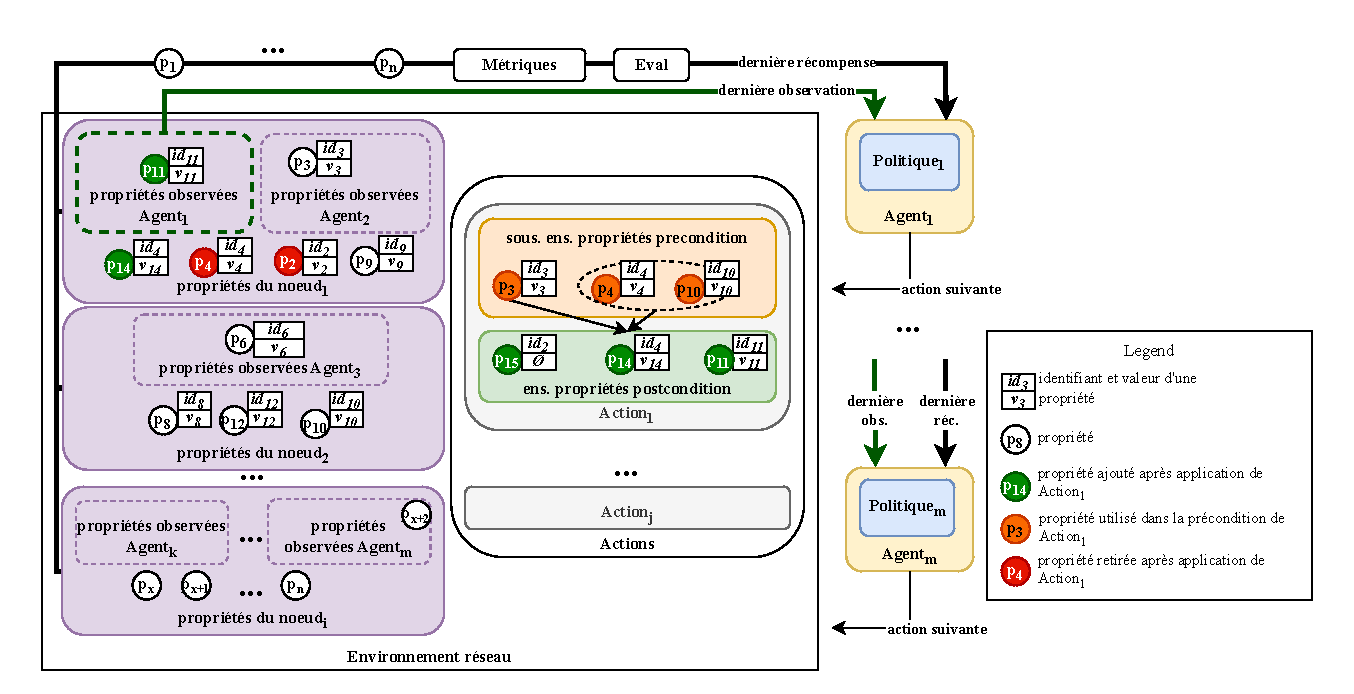
\includegraphics[width=0.97\textwidth]{figures/model_example_illustration.pdf}
    \caption{An illustrative view of the simulation model}
    \label{fig:model_example_illustration}
\end{figure*}

\noindent
From a global view the proposed Dec-POMDP model expresses an environment state as the set of nodes properties including agents observable properties. We define a property as a couple made of an identifier and a value. The environment state is changed when an action is applied by an agent. An action can be applied only if the boolean property-based pre-condition is satisfied in the current environment state. The resulting state is then modified depending on post-condition ultimately leading some new properties to be added while some others are deleted. After an action is successfully applied by an agent, observable properties of the same agent are returned to it as observations from that new state. A reward is also computed based on the current state and returned to the agent. An agent is chosen to be modeled as a behavior function which has to select the next action to be made depending on received observations and rewards.

There are different ways for several agents to be executed in a same environment tweaking with the number of agents to execute in a time step and the number of actions to be played by an agent in a time step. Even though not realistic, we chose the \textquote{Agent Environment Cycle}~\cite{jk2020} as a first approximation by having several agents playing one action in each turn in a sequential cyclic manner. The iteration cycle is presented through an illustrative informal view of the simulation model in Figure~\ref{fig:model_example_illustration}. It shows $i$ nodes with their properties including the $m$ agents' observed ones; and how each of the available $j$ actions associates a pre-condition set of properties subsets to a subset of new properties to be added in the environment optionally deleting obsolete properties having the same identifiers as the new properties' ones: \begin{enumerate*}[label=\arabic*),itemjoin={;\quad}]     
    \item An agent chooses an action from previous observations and rewards according to a behavior function. In Figure~\ref{fig:model_example_illustration}, as $Agent_1$ begins its first turn, it receives only initial observations ($p_{1}$) and zero rewards and chooses $Action_1$
    
    \item The environment is updated by a transition function depending on the current state and the action taken by the agent (change of properties once the pre-condition is satisfied). An action is used to change the environment properties by updating the relation between property identifiers and property values.
    For instance, in Figure~\ref{fig:model_example_illustration}, in current state, $Node_1$ properties are $p_1,p_3,p_4,p_2,p_9$. When $Action_1$ is applied, the relation associate subsets $\{p_3\}$ or $\{p_4, \allowbreak p_{10}\}$ to $\{p_{15}, \allowbreak p_{14}, \allowbreak p_{11}\}$. The property based pre-condition can be understood as $p_3 \lor (p_4 \land p_{10})$. As $p_{15}$ and $p_{14}$ are identified by $ID_4$ and $ID_2$ which already respectively define $p_{2}$ and $p_{4}$, $p_{4}$ and $p_{2}$ are deleted and $p_{11}$ and $p_{14}$ are added ($p_{15}$ is not added as $id_2$ is not associated with any value)
    
    \item Observed properties are returned to the current executor agent for its next turn. In Figure~\ref{fig:model_example_illustration} $p_{11}$ and $p_1$ are returned after $Action_1$ is applied.

\end{enumerate*}

\noindent
Agents are selected following a sequential order. Each one receives last observations and rewards from their last turn (or just initial observation and zero rewards if they are on their first turn); chooses the next action to play in its current turn. Once the last agent has finished playing (such as $Agent_m$), rewards are computed and sent to cyber-attackers and cyber-defenders based on the evaluation of the collected metrics from last state. Then, the agents play again following the same sequential order for another iteration.


\subsection{Formal Dec-POMDP modeling}

We set the elements related to the properties of the nodes, agents and actions of the following environment:

\begin{itemize}

    \item $Ag = \{ag_1,..,ag_{|Ag|}\}$: The set of agents (cyber-attackers and cyber-defenders).
    % \begin{itemize}
    %     \item With $Attackers \subseteq Ag$: The set of attacker agents
    %     \item With $Defenders \subseteq Ag$: The set of defender agents
    % \end{itemize}

    \item We call the couple $p = (id_{j}, v_{j})$ with $id_j \in {ID}$ and $v_j \in V$, a property.
    \begin{itemize}
        \item $ID$: The set of property identifiers optionally indicating how are organized the properties in a non-flat data structure (such as $PC1.processes.agents.agent1$). These property identifiers may be used for a file path, the type of operating system used in a node, a used command line by an agent\dots
        \item $V$: The set of property values. These may include the content of a file, a full description of the operating system, the output result of a command line\dots
        % \item $Values: ID \rightarrow \mathcal{P}(V) = \{(id_{j}, V_{j}) \: | \: id_j \in {ID},$ $V_j \in \mathcal{P}(V)\}$: a bijection associating a property identifier to the set of the different values it can be associated with. For instance, a the identifier $ls\_command\_output$ may be associated with the following values $\{file.txt,\{file.txt,passwd.txt\}\}$
    \end{itemize}

    \item $P_{j} = \{ p_1, .., p_{|P_{j}|} \}$: The set of the $p_{l}$ properties (with $l \in \{1,..,|P_{j}|\}$) of node $j$ ($j \in \mathbb{N} $). For example, such properties may include some running process IDs, files list in a folder, type of operating system with description, specific knowledge of an agent, etc.
    \begin{itemize}
        \item $P = P_1 \cup P_2 .. \cup P_{|P|} $: The set of all the node properties.
    \end{itemize}

    \item $Obs: \mathcal{P}(P) \times Ag \rightarrow \mathcal{P}(P_{Ag}), P_{Ag} \subset P$: A relation which associates node properties and an agent with the observed property subset by the agent.
    
    \item $Action: P_{pre} \rightarrow P_{post}$: A relation which associates a property subset implied by an equivalent conjunctive boolean pre-condition ($P_{pre} \subset \mathcal{P}(P)$) to a subset of all of the properties of the post-condition ($P_{post} \in \mathcal{P}(P)$). For example, the properties $p_1 = (agent\_X\_privilege\_level, \allowbreak root)$, $p_2 = (agent\_X\_accessed\_text\_editor, \allowbreak Vim)$ and $p_3 = (agent\_X\_bashrc\_known\_filepath, \allowbreak /home/user/.bashrc)$ can make a pre-condition ($p_1 \land p_2 \land p_3$) to associate a new set of property containing $p4 = (bashrc\_file\_modified\_by\_X\_agent, \top)$. Two pre-condition subsets can be associated to the same post-condition subset to model a boolean disjunction.

    \item $Metrics: \mathcal{P}(P) \times A \rightarrow \mathbb{R}^{n}$: Gives metrics associated with a set of properties and joint action. For example, the number of nodes still active, lateral moves, etc.

\end{itemize}


Using the formal description of a Dec-POMDP~\cite{OliehoekA16}, we propose the following model:

\begin{itemize}
    \item $S = \{s_1, ..s_{|S|}\}, s_{i} \subseteq P \: and \: 1 \le i \le |S|$: The space of states as possible property sets.

    \item $A_{i} = \{a_{i}^{1},..,a_{i}^{|A_{i}|}\}, a_{i}^j \in Action \: and \: 1 \le j \le |A_i|$: The set of possible actions for agent $i$.

    \item $T$ : The set of conditional transition probabilities between states
    \begin{itemize}
        \item With $T(s,a,s') = \probP(s'|s,a)$, the relation which associates probability to go to state $s' \in S$ from state $s \in S$ knowing we played $a = (P^a_{pre} \times P^a_{post}) \in A$ with $P^a_{pre} \subset \mathcal{P}(P)$ and $P^a_{post} \in \mathcal{P}(P)$
        \item With $\probP(s'|s,a) = 0$ if $s$ does not satisfy the pre-condition of $a$ (i.e $\exists \: P_{pre_s}^{a} \in P_{pre}^{a} \: | \: P_{pre_s}^{a} \not\in \mathcal{P}(s)$).
        \item With $s' = (s - \{p_l=(id_l, v_l) \: | \: p_l \in s \: and$ $id_l \in \{id_k \: | \: (id_k, v_k) \in P^a_{post} \: and \: v_k \neq \varnothing\}\}) \cup P^a_{post}$
    \end{itemize}
    
    \item $R: S \times A \rightarrow \mathbb{R}^2 = Eval \circ Metrics$: The reward function that takes a state and an action and associates a performance indicator (using the state's metrics) for attackers and defenders.
    \begin{itemize}
        \item With $Eval: \mathbb{R}^{n} \rightarrow \mathbb{R}^2$, associates a metric vector to a a reward for cyber-attackers and cyber-defenders.
    \end{itemize}
    
    \item $\Omega_{i} \subset Range(Obs \: | \: \{ (s, ag_i) | s \in S \: and \: ag_i \in Ag \}) \subset P$: The set of observable properties for agent $ag_i$. For example, the content of a file, the log output of a command, the result of a port scan, etc.
    \begin{itemize}
        \item $\Omega = \Omega_1 \cup \Omega_2 .. \cup \Omega_{|Ag|} = Range(Obs)$: The set of all the observable properties for all agent.
    \end{itemize}

    \item $O$ : The set of conditional observation probabilities.
    \begin{itemize}
        \item With $O(s',a,o) = \probP(o|s',a)$, the relation which associates the probability to observe an observation $o \subset \Omega$ from state $s' \in S$ induced by $a \in A$
        \item With $\probP(o|s',a) = 0$ if the state $s' \in S$ does not contain the properties of $o \subset \Omega$ (i.e $o \not\in \mathcal{P}(s')$). For example, an agent plays the action $x\_reads\_a\_log\_file$, a new state results from which a property belonging to the knowledge of agent x is $(log\_file\_content\_known\_by\_x, \allowbreak abc)$. This property will be therefore included in the returned observations to agent x. 
    \end{itemize}

\end{itemize}


\subsection{Attack/defense scenarios integration\label{sec:ad_integration}}

\noindent
From a raw perspective, the proposed formal Dec-POMDP modeling relies on actions to simulate how a real networked system would react including vulnerabilities and countermeasures applied by cyber-attacker and cyber-defender agents.

A first challenge is to build a representative attack/defense scenario of a networked system comprising vulnerabilities to allow rendering an attack by linking the only available pieces of information (such as known tactics, techniques and procedures from MITRE ATT\&CK) and by choosing relevant defense countermeasures (from MITRE ATT\&CK mitigations) and a deployment environment. A second challenge is to establish the actions to match the attack/defense scenario. As actions modify the environment properties, they also impact possible states space and the transitions between them.
Moreover, when considering a low abstraction level, numerous simple actions may allow describing the operated changes in the network finely. Yet, doing so increases the number of actions, and even more the number of states for they are combinations of action effects.

These challenges are directly linked to studied issues about automated generation of attack graphs using available databases optionally integrating artificial intelligence techniques as in ~\cite{GFalco2018}. We do not intend to focus more on these issues as they are out of the scope of this work.

\

\noindent
\textbf{MITRE ATT\&CK integration approach}: We suggest a high-level manual approach we used to integrate MITRE ATT\&CK information as an AD tree for it formalizes actions to be played in a scenario and their interactions with the environment. It is aimed at being helpful to establish the attack/defense actions to be finally integrated in the simulator:
\begin{enumerate*}[label=\arabic*),itemjoin={;\quad}]

    \item For a given Advanced Persistent Threat (APT), we identified relevant tactics and techniques and procedures from MITRE ATT\&CK that seemed relevant for a networked system
    
    \item We produced a description linking identified tactics together and associated techniques, sub-techniques and procedures to create a scenario that describes how the APT group could attack the networked system. This step defines the network topology with its main properties
    %(such as a company network made up of several dedicated database servers communicating through FTP and HTTP, etc.)

    \item We created an AD tree as proposed in ~\cite{BKordy2010} with tactics as top action goals while techniques, sub-techniques and procedures are in the lower part of the tree. We made sure to have several paths to reach a same top-action goal. We paid attention to define each attack action with property based pre-condition and property post-conditions in the environment

    \item We extracted the MITRE ATT\&CK techniques/sub-techniques related detection and mitigations we added in the AD tree to decorate the attack nodes. We paid attention to define each defense actions with property based pre-condition and property post-conditions in the environment.



    % \item We also listed and defined the main deployment specific environmental actions from deployment environment previous description or extended attack/defense actions which are common to both cyber-defenders and cyber-attackers. This step brings a more realistic environment providing a representative number of plausible actions an agent can choose in many systems.
    % These common actions could include at least:
    % \begin{itemize}
    %     \item Reading and writing files
    %     \item Creating, deleting, copying, moving, renaming, modifying properties of files/folders.
    %     \item Go into a folder, go to the parent folder
    %     \item Focusing a file/folder for applying future actions
    %     \item Execute binary file
    %     \item Using network protocol (such as HTTP, FTP, SSH, etc.).
    %     \item Some other interactions with basic command lines about system monitoring or controlling.
    % \end{itemize}
    % Then, associated environmental properties should describe a file system, a terminal interface, port with rules, operating system parameters properties, etc.

\end{enumerate*}

\subsection{Simulation model implementation}

\noindent
Potential works to implement our model include: NeSSi2~\cite{DGrunewald2011} which is an agent-based simulation platform aiming to model only packet-level description of a networked system and the effects of DDoS attacks; and Kotenko et al.~\cite{IKotenko2007} which relies on OMNet++~\cite{Varga2010} to model and simulate cooperative cyber-defense agents against network attacks combining discrete-event simulation, multi-agent approach and packet-level simulation of network protocols.
% Additionally, to overcome limited realism, emulators using virtual machines and integrated with offensive tools have been pushed forward, such as DCAFE~\cite{GRush2014} and SVED~\cite{HHannes2016}.
However, among these, none can fully meet both the consideration of a multi-agent cyber environment for a Dec-POMDP model.
%and the need for code accessibility (open source code).

\begin{figure}
    \centering
    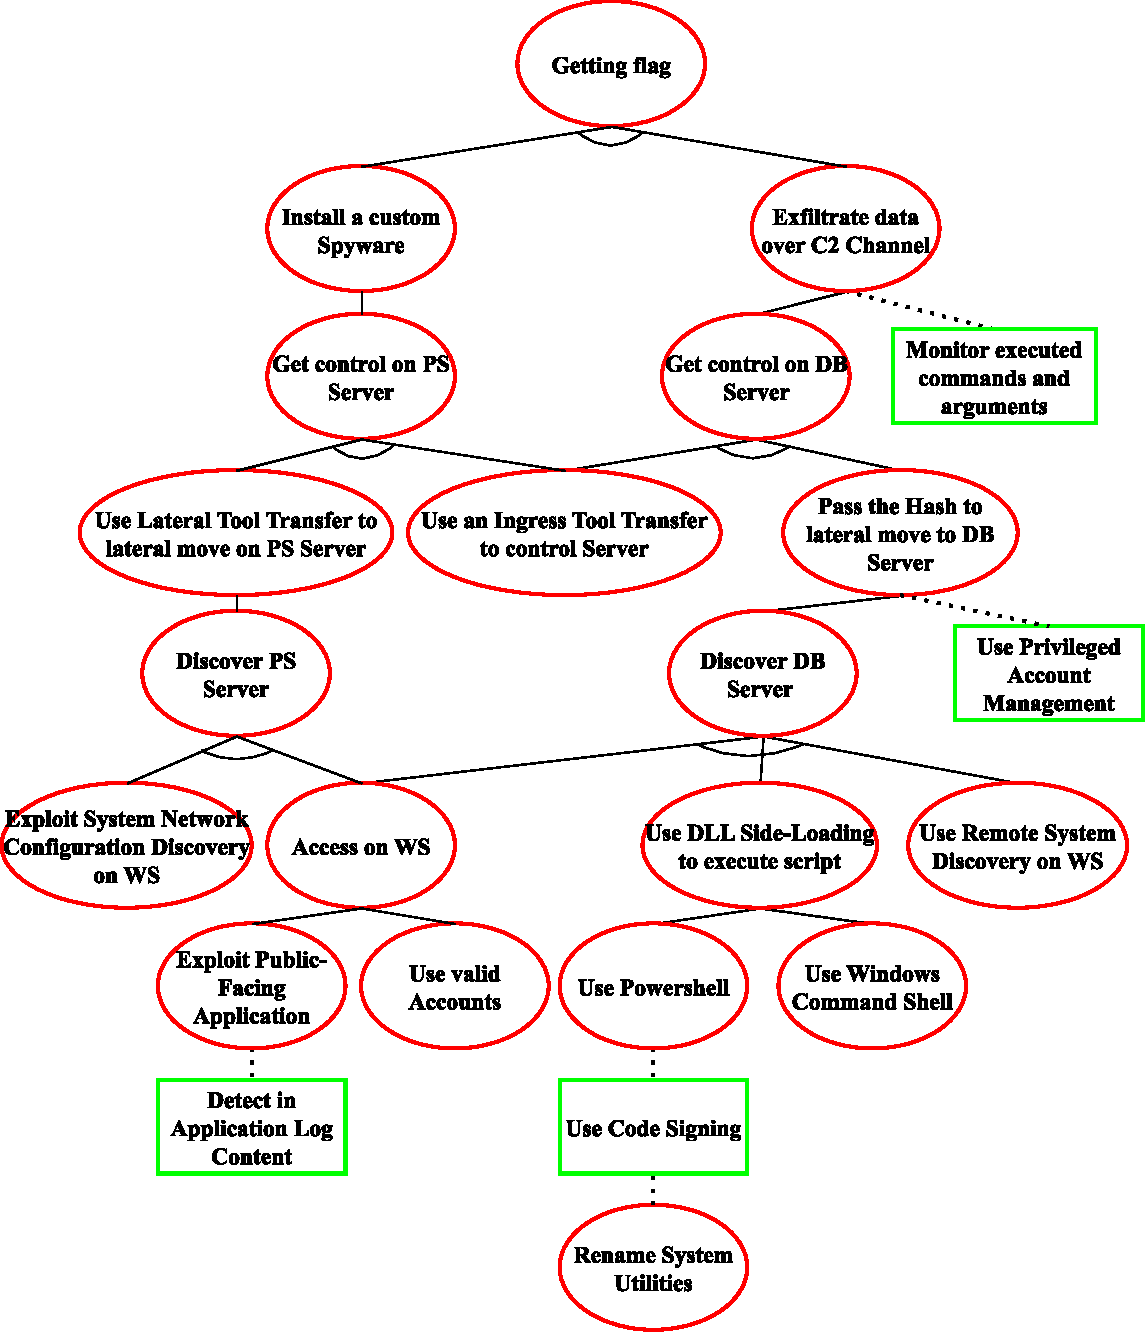
\includegraphics[width=\linewidth]{figures/ADTree.pdf}
    \caption{An overview of the proposed attack/defense AD Tree}
    \label{fig:ADTree}
\end{figure}

Yet, we identified discrete-event simulators with a single cyber-attacker such as CYST\cite{drasar_session-level_2020} or CyberBattleSim~\cite{cyberbattlesim}, which both provide a suited network simulation and evaluation approach towards an implementation of our model as their underlying models can be extended for several agents. Inspired by these approaches, we used \textit{PettingZoo}~\cite{jk2020} as a fundamental platform to implement our Dec-POMDP model onto which we aimed to implement a simulated network. \textit{PettingZoo} provides a framework where the designer has tools to facilitate the implementation of the space of observations, actions, management of agents at each turn and associated rewards.

% \begin{figure}
%      \centering
%      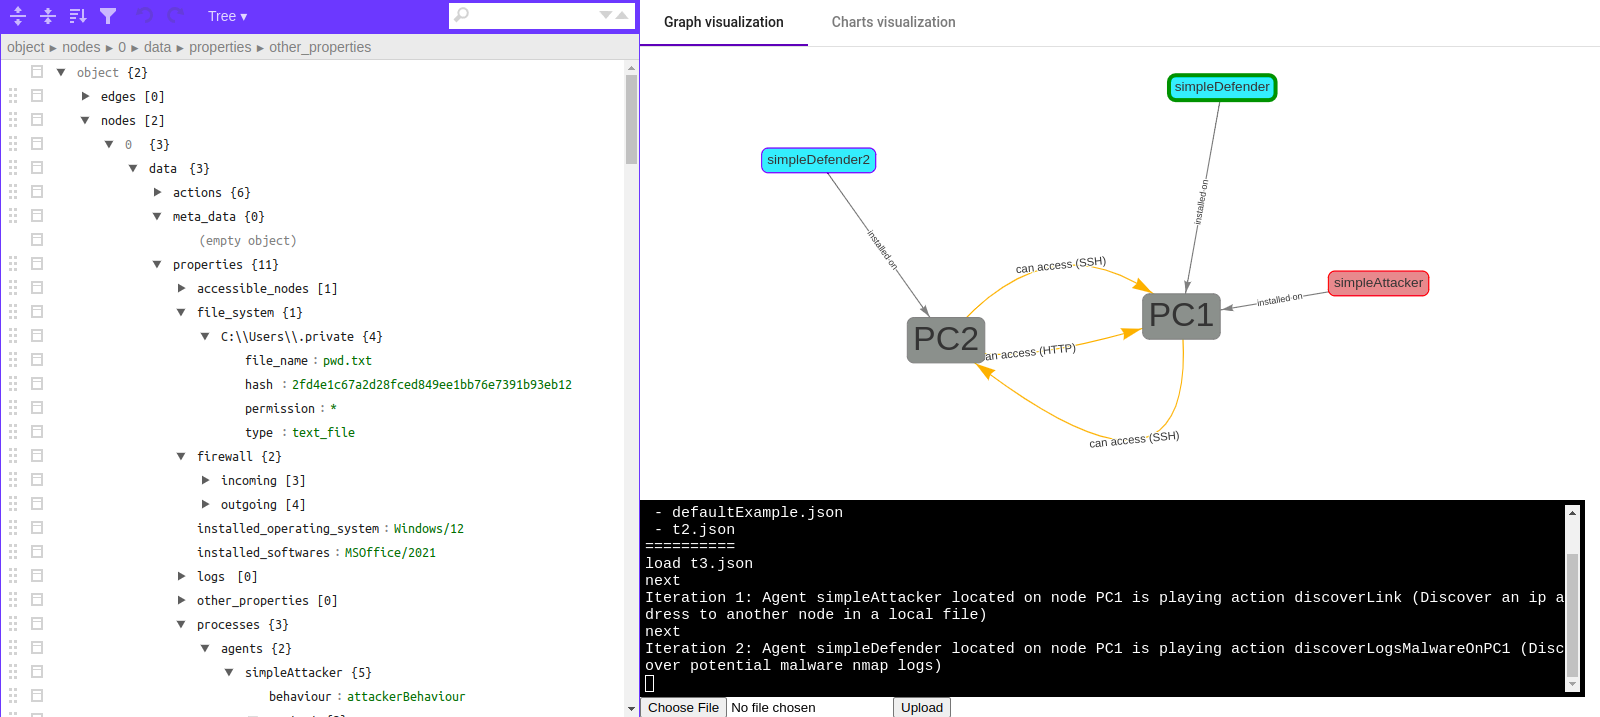
\includegraphics[width=\linewidth]{figures/interface_MCAS.png}
%      \caption{Simulator interface overview}
%      \label{fig:simulator_interface}
% \end{figure}

The development of our model has led to the \textquote{Multi Cyber Agent Simulator} (MCAS)~\cite{MCASWebsite} simulator. In the current state of development, this simulator allows loading/saving a \textit{json} file describing the nodes properties and actions of the environment and the defined agents with their behaviors; and launching the execution of the agents of this environment in turn-by-turn mode via the terminal. It is possible to view the environment properties in real time and visualize the environment in the form of a graph. Metrics are displayed as well.



\section{MITRE ATT\&CK based case study}

% \rem{Expliquer pourquoi on veut tester les capacités du simulateur -> illustration de comment fonctionne le simulateur}
% \rem{Gallium APT, pourquoi ce choix ? pourquoi ce cas d'étude inspiré de ça ? Qu'est-ce qui est interessant dans Gallium APT ? Type d'attaque/ coordination d'attaque ?}

\noindent
Intending to assess coordinated attacks and collective defense, we chose GALLIUM APT (a cyberespionage group active since 2012), for it allows defining several concurrent attacks.


\subsection{Network topology}

% \rem{Pour chaque élément présent dans la figure, faire le lien avec les éléments cités dans la présentation de la topologie...}

\noindent
Based on some GALLIUM APT tactics we selected some associated techniques/sub-techniques to propose a small company like networked environment, presented in Figure~\ref{fig:scenario_network_topology}. It is divided in 5 subnets communicating through implicit routers positioned after a firewall:
The outside subnet used to represent external attackers as if in the same network for convenience. It includes two desktop computers (At1 and At2).
The Demilitarized Zone (DMZ) subnet is used to separate devices that are accessible from the Internet from the rest of the company's network. The servers in the DMZ include a web server (WS), an email server (ES), a VPN server (VPN), and a FTP server (FTP), all connected bidirectionally both to outside and inside the company network.
The first local area network (ACC) subnet used to connect devices within the accounting department of the company where employee are working in. It contains two employee workstations (E1 and E2) and a Chief Technical Officer workstation (CTO), all connected bidirectionally to the DMZ. % and only accessible from SRV (defined below);
The second local area network (MAR) subnet used to connect devices within the marketing department of the company. It contains a printer server (PS), one employee workstations (E3) and tablet terminal (TAB) connected via a wireless access point, all connected bidirectionally to the DMZ. %and only accessible from SRV (defined below);
The third local area network (SRV) subnet used to connect the company devices providing services. It contains an API server (API), a database server (DB), and a domain controller (DC).

\begin{figure}
    \centering
    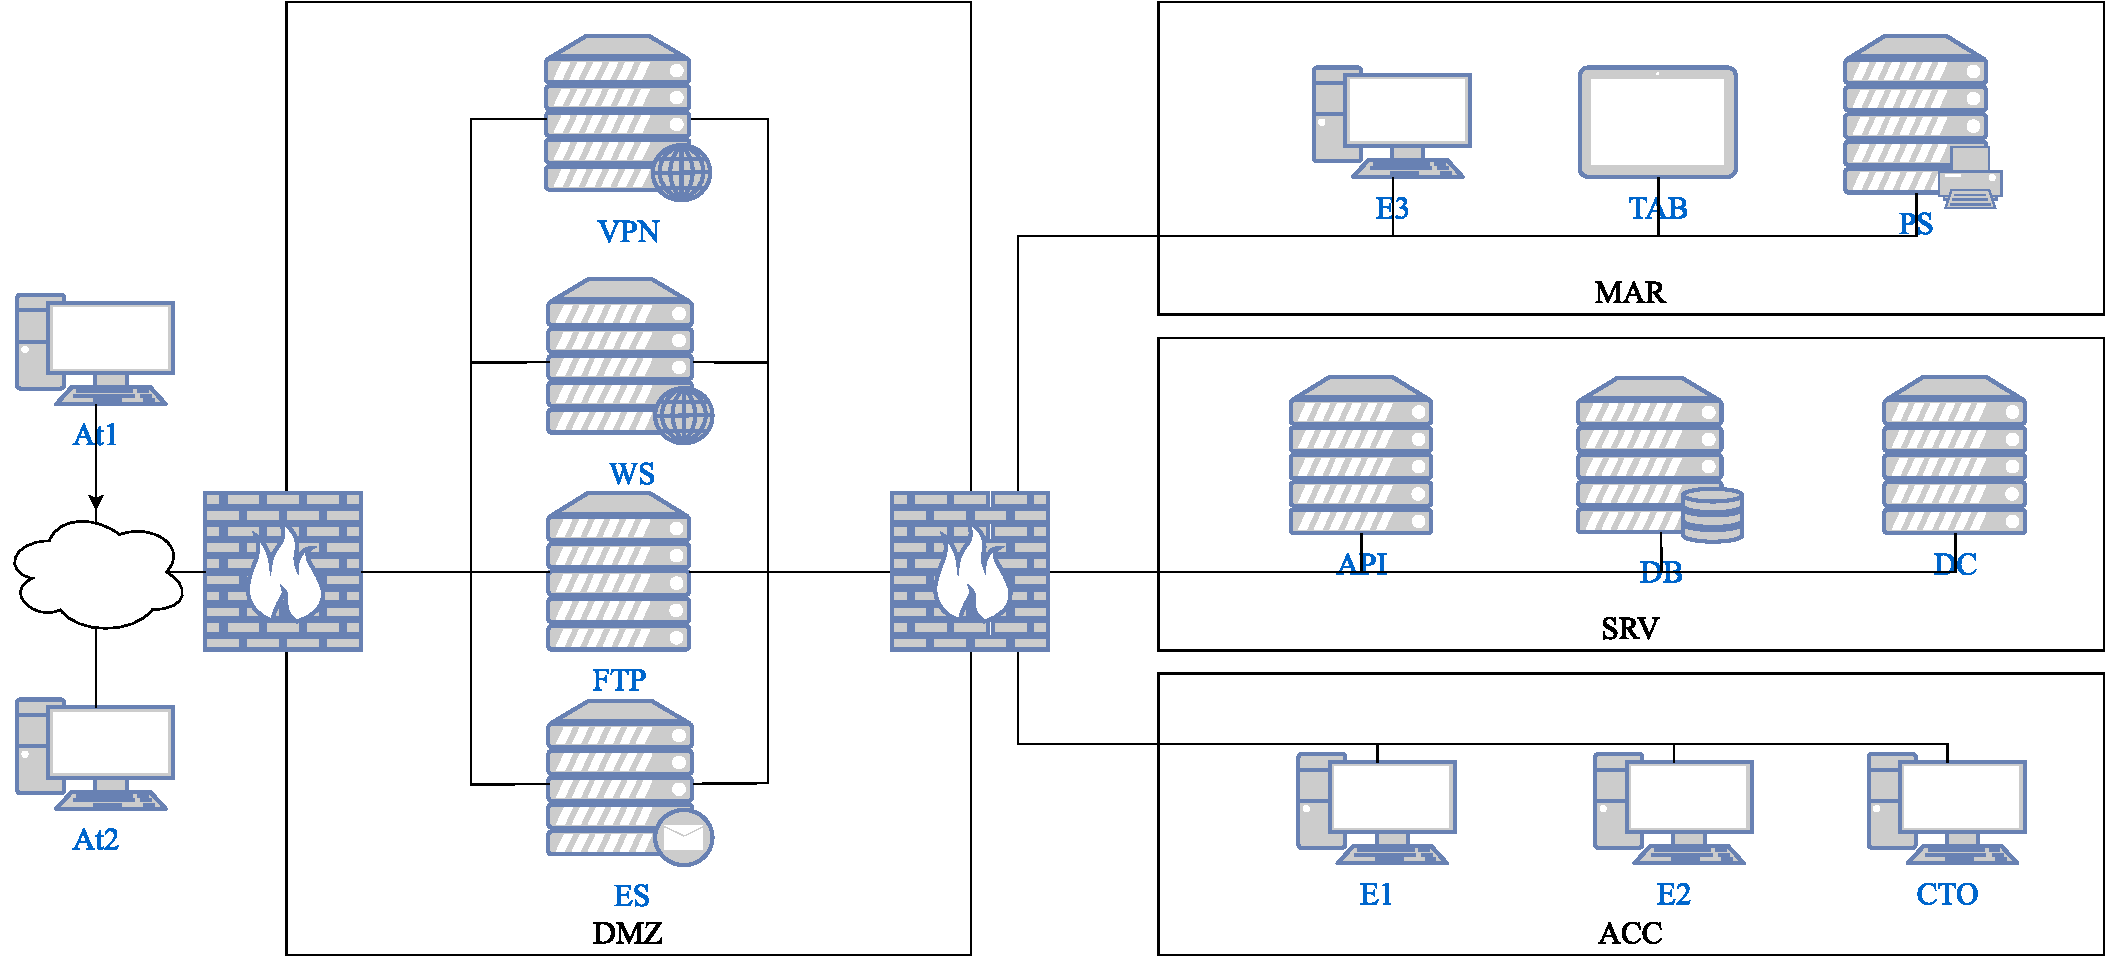
\includegraphics[width=\linewidth]{figures/topology.pdf}
    \caption{Proposed small-scale company network topology}
    \label{fig:scenario_network_topology}
\end{figure}


%These devices are accessible from the DMZ and from the CTO. API is also accessible via a VPN tunnel from the outside.

% The simulated machines are populated with files, folders, firewall rules, network services, and so on, so both attackers and defenders can have more actions to interact.


\subsection{Scenario and agent implementation with evaluation}

\begin{figure}
    \centering
    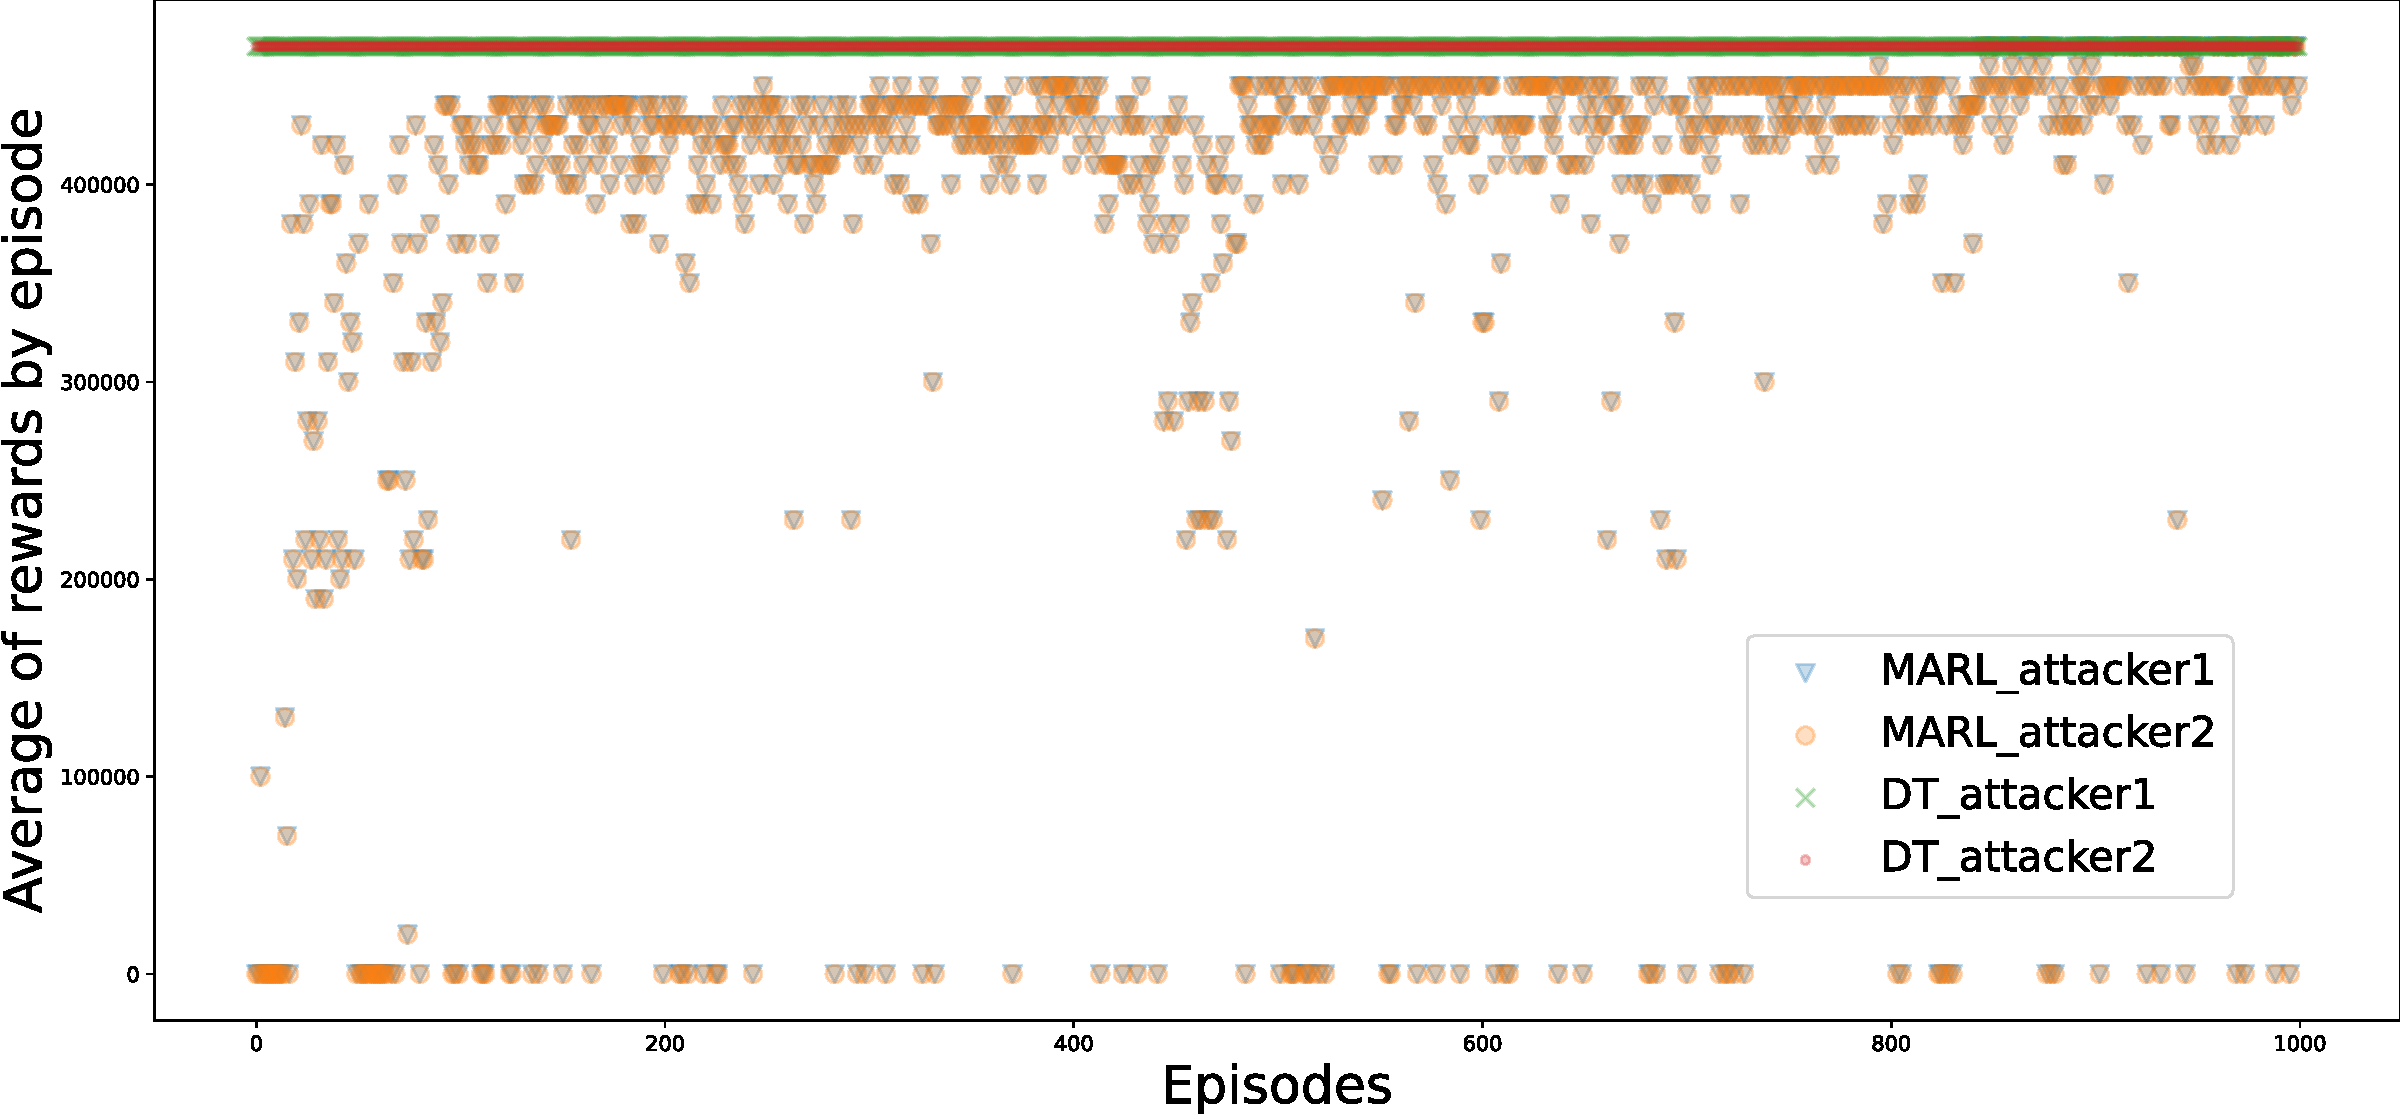
\includegraphics[width=\linewidth]{figures/graphs.pdf}
    \caption{An evolution of the rewards average according to episodes in small-scale tests with MARL and Decision Tree Approaches with inactive cyber-defense
    }
    \label{fig:graphs}
\end{figure}

\noindent
The cyber-attacker agents are initially deployed on At1 and At2 and the cyber-defender agents are deployed on WS and DB. The ultimate attackers' goals is to get data from the DB server and installing one spyware on the printer server PS. Following our approach in ~\ref{sec:ad_integration} we propose an AD tree presented in Figure~\ref{fig:ADTree}. It only shows the paths of the attacks to follow to reach the ultimate goal while the defender actions can prevent these at several stages of the attack.
We first interested in setting up the two cyber-attackers behaviors, then the two cyber-defenders' ones. We simulated an abstracted version of the scenario over 1000 episodes.

% In addition, we implemented some other common actions to interact with the file system, OS configuration, firewall configuration, and network services. These actions can be derived from the attack/defense actions but are implicitly not shown in the AD tree. Yet, they are taken into account in the simulation so agents can explore action paths even if this does not lead to an ultimate attacker goal.


%\subsection{Scenario execution and evaluation}

\noindent
\textbf{Random approach}: \quad The random agent only choose its actions by exploring the whole action space without any criteria until reaching the goal. In our case study, the shortest action path for attackers to reach the ultimate goal contains 16 different actions among the 30 defined actions, hence a low probability of $(1/30)^{16}$.
This approach allows getting a benchmark of unexpected edge failure cases and to compare with other types of agent.

\noindent
\textbf{Decision Tree (DT) approach}: \quad The decision tree was applied to get a reference when cyber-attackers or cyber-defenders already know the best action to take as the role of each agent is defined by a DT.
In Figure~\ref{fig:graphs}, the $DT\_attacker1$ follows an action path to reach the goal of installing a custom spyware in PS. In the same time, $DT\_attacker2$ reaches the goal of exfiltrating data in DB and completing the action path by getting the flag. Then we added the defenders $DT\_defender1$ which has to detect malicious logs on WS and $DT\_defender2$ which has to use privilege account management or monitor the executed commands and arguments on DB. We observed the attackers to be unable to reach the ultimate goal.

\noindent
\textbf{Multi-Agent Reinforcement Learning (MARL) approach}: \quad Q-Learning~\cite{CWatkins1992} was applied with curriculum learning for first the attackers learn how to reach the ultimate attack goal before adding defenders.
In the Figure~\ref{fig:graphs}, $MARL\_attacker1$ and $MARL\_attacker2$ follow a same behavior ultimately refining the applied actions to the relevant ones to reach the ultimate goal. After several episodes, chosen action paths by the attackers tend to be as efficient as the DT paths. When adding the defenders $MARL\_defender1$ and $MARL\_defender2$, we verified the attackers to be less and less able to reach the ultimate goal.


\section{Conclusion and perspectives}

\noindent
We proposed a Dec-POMDP modeling of networked node likely to be attacked and defended by agents. This model aims to integrate scenarios. The implementation of this model led to a simulator whose some capabilities have been assessed through a MITRE ATT\&CK scenario. Using three approaches, we briefly checked how decision tree, random and reinforcement learning approaches can be applied to agent for comparison.
Willing to take advantage of this simulation approach to address realistic issues related to cyber-defenders, particularly in the AICA context, we identified the main limitations to overcome:
automating the integration of more realistic scenarios leveraging on a basis of common actions and properties so agents can explore and act as in seemingly similar to reality information systems;
establishing a way to use the benefits of results obtained with simulations for emulated or real systems while maintaining agent behaviors during deployment;
having more coordination between agents, such as several entry points or scenarios with needed communication to reach a goal\dots;
and introducing new constraints in actions (such as cost, execution duration, etc.).


\noindent L'\textit{activité de modélisation} a pour objectif de représenter le problème de conception comme un problème d'optimisation sous contraintes. Pour cela, la tâche la plus difficile est de modéliser l'environnement comme un modèle assimilable à une simulation avec un niveau de fidélité connu. Deux approches sont envisageables pour faciliter cette tâche :
\begin{itemize}
    \item Dans le cadre de la Cyberdéfense, la modélisation manuelle d'un environnement, telle que l'infrastructure en réseau d'une entreprise par une analyse manuelle de l'environnement réel pour obtenir une version simplifiée. Cependant, en raison de l'inexistence de modèle générique servant de chassis pour la modélisation d'un tel environnement, ce travail peut être fastidieux et conduire à différents modèles peu homogènes. C'est pourquoi nous proposons un modèle formel générique pouvant servir de base à la modélisation d'un environnement.
    \item La génération automatisée d'un environnement. Cependant, en raison de l'impossibilité d'accéder directement à l'état réel de l'environnement, nous nous appuyons sur les historiques conjoints stockés. C'est pourquoi nous utilisons les World Models, capables de généraliser à partir d'un grand volume d'historiques pour estimer les transitions d'états cachés et d'observations. Toutefois, un obstacle majeur est l'absence de World Models explicitement conçus pour les environnements multi-agents. Nous proposons ci-dessous une extension du cadre World Models aux contextes multi-agents.
\end{itemize}

En complément de cet environnement simulé, le problème d'optimisation formalisé comprend également la transformation de la description informelle de l'objectif global $\mathcal{G}_{\text{inf}}$ en une fonction de récompense basée sur l'historique $R^j_H: H^j \times \Omega^j \rightarrow \mathbb{R}$, ainsi que la formalisation des contraintes issues des exigences de conception $\mathcal{C}_{\text{inf}}$ sous la forme de spécifications organisationnelles MOISE+MARL $\mathcal{MM}$.

Nous supposons ici que la formalisation manuelle de la description informelle de l'objectif et des contraintes de conception en une fonction $R^j_H$ et en spécifications $\mathcal{MM}$ est prise en charge.



\subsubsection*{Extension aux World Models Multi-Agents}

elle commence par générer un environnement simulé de haute fidélité en construisant un \acn{JOPM} $\mathcal{T}^j : H^j \times \Omega^j \times A^j \rightarrow \mathcal{H} \times \hat{\Omega}^j$ à partir des traces d'interactions réelles $\mathcal{D}_{H^j}$. À un pas de temps $t \in \mathbb{N}$, pour tout état caché récurrent $\tilde{h}_{t-1} \in \mathcal{H}$ représentant l'historique conjoint jusqu'à $t-1$, l'observation conjointe reçue $\omega_t^j \in H^j$ et l'action conjointe $a_t^j \in A^j$, le modèle $\mathcal{T}^j$ renvoie le nouvel état caché $\tilde{h}_t \in \mathcal{H}$ ainsi que la prédiction de la prochaine observation conjointe $\hat{\omega}^j \in \hat{\Omega}^j$. Ce mécanisme permet à \acn{MAMAD} de construire l'environnement de simulation depuis zéro.

Dans les environnements multi-agents, les observations conjointes deviennent rapidement de grande dimension à mesure que le nombre d'agents augmente. Pour pallier cela, des fonctions d'encodage conjoint sont introduites pour les observations et les actions.

Plus précisément, les observations conjointes $\omega_t^{j} = (\omega_t^1, \dots, \omega_t^n) \in \Omega^{j}$ sont transformées en représentations latentes compactes à l'aide d'un encodeur d'observations conjointes $Enc_{\omega^j} : \Omega^j \rightarrow z$, produisant $z_t = Enc_{\omega^j}(\omega_t^j)$. Un décodeur $Dec_z : z \rightarrow \hat{\Omega}^j$ permet la reconstruction des observations conjointes si nécessaire.

On utilise généralement des \acn{MLP}s ou des architectures à base d'attention pour ces encodeurs, afin d'agréger les informations multi-agents en vecteurs de caractéristiques de taille fixe, tout en capturant les dépendances critiques entre agents.

Une fois l'encodage effectué, le World Model multi-agent fonctionne comme en contexte mono-agent, en utilisant les observations encodées $z_t$ dans les historiques transmis au \acn{RLDM} $\mathcal{T}^{z}$. Ce modèle permet une modélisation évolutive, tout en conservant les motifs d'interaction clés entre agents. Dans le cadre de \acn{MAMAD}, ces World Models constituent le cœur de la simulation mise en œuvre par l'\hyperref[sec:modelling]{activité de modélisation}, agissant comme des jumeaux numériques de haute fidélité de l'environnement cible.

\begin{algorithm}[H]
    \caption{Algorithme de l'activité de modélisation}
    \label{alg:modeling}
    \DontPrintSemicolon

    \KwIn{Historiques conjoints $\mathcal{D}_{H^j}$, objectif informel $\mathcal{G}_{\text{inf}}$, contraintes informelles $\mathcal{C}_{\text{inf}}$, facteur d'actualisation $\gamma$, espace des actions $A$, espace des observations $\Omega$}
    \KwOut{JOPM $\mathcal{T}^j$, fonction de récompense $R^j_H$, spécifications MOISE+MARL $\mathcal{MM}$}

    \vspace{0.5em}
    \tcp{1. Formalisation manuelle des exigences symboliques}
    $R^j_H \gets \texttt{manual\_formalize}(\mathcal{G}_{\text{inf}})$ \;
    $\mathcal{MM} \gets \texttt{manual\_formalize}(\mathcal{C}_{\text{inf}})$ \;

    \vspace{0.5em}
    \tcp{2. Entraîner les encodeurs pour les observations et actions conjointes}
    Extraire les observations $\Omega^j = \{\omega^j_t\}$ à partir des historiques $\mathcal{D}_{H^j}$ \;
    Entraîner un auto-encodeur $(Enc_{\omega^j}, Dec_{\omega^j})$ sur $\Omega^j$ en minimisant l'erreur de reconstruction \;

    \vspace{0.5em}
    \tcp{3. Encoder les observations dans les historiques}
    Pour chaque historique $h^j = \{\omega_t^j, a_t^j\} \in \mathcal{D}_{H^j}$, encoder chaque observation conjointe ${z}_t = Enc_{\omega^j}(\omega^j_t)$ pour constituer l'ensemble d'entraînement $\mathcal{B} = \{ \{(z_t, a^j_t, z_{t+1})\} = h_z^j, h_z^j \in \mathcal{D}_{H^j}\}$

    \vspace{0.5em}
    \tcp{4. Entraîner le RLDM}
    Initialiser le RLDM (fonctions $f$ et $g$) $\mathcal{T}^z = f(g)$

    \For{$h_z^j \in \mathcal{B}$}{
        \For{$(z_t, a^j_t, z_{t+1}) \in h^j$}{
            Entraîner le RLDM $\mathcal{T}^{z}$ en minimisant l'erreur quadratique moyenne (MSE) entre la prédiction $\hat{z}_{t+1}$ et la valeur réelle $z_{t+1}$.
        }
    }

    \vspace{0.5em}
    \tcp{5. Sauvegarder les observations initiales et former le JOPM}

    $\Omega^{\mathcal{T}^j}_0 \gets \{\omega^j_0\}$ extraites des historiques $\mathcal{D}_{H^j}$

    $\mathcal{T}^j(h_{t-1}, \omega_t, a_t) = \langle f(h_{t-1}, Enc(\omega^j_t), a^j_t), Dec(\mathcal{T}^{z}(h_{t-1}, Enc(\omega^j_t), a^j_t)) \rangle$ \;

    \vspace{0.5em}
    \tcp{6. Retourner les éléments modélisés}
    \Return{$\mathcal{T}^j, \Omega^{\mathcal{T}^j}_0, R^j_H, \mathcal{MM}$}
\end{algorithm}


\chapter{Entraînement des politiques sous contraintes}
\label{chap:training}

L'\textbf{activité d'entraînement} traite les éléments formels suivants :
%
\begin{displaymath}
    \pi^j_i \gets \texttt{train}(\mathcal{T}^j, \Omega^{\mathcal{T}^j}_0, \gamma, R^j_H, \Omega, A, \mathcal{MM})
\end{displaymath}

L'\textit{activité d'entraînement} vise à résoudre le problème de conception modélisé comme un problème d'optimisation sous contraintes en s'appuyant sur le cadre MOISE+MARL. Cependant, une limite importante réside dans le fait que MOISE+MARL repose sur le formalisme \acn{Dec-POMDP}, qui suppose un accès complet à l'état réel de l'environnement. En pratique, notre approche se fonde uniquement sur les données observables (à savoir les historiques conjoints des agents) sans accès aux états internes. Pour combler cet écart, un nouveau formalisme markovien est introduit, opéré sur des séquences observables via le \acn{JOPM}, tout en restant compatible avec les cadres algorithmiques \acn{MARL} existants.

\subsubsection{Extension de MOISE+MARL aux World Models Multi-Agents}

\noindent Dans des environnements réalistes, on ne dispose que des transitions issues des historiques d'actions et d'observations reçues. Pour mieux représenter ce contexte, nous introduisons un nouveau formalisme appelé \textbf{Dec-POMDP basé sur les observations} (\acparen{ODec-POMDP}).

Un \acn{ODec-POMDP} $d_\Omega \in OD_\Omega$ (où $OD_\Omega$ désigne l'ensemble des ODec-POMDPs) est défini comme un quintuplet :
%
$d_\Omega = \left(\Omega, A, \mathcal{T}^j, R^j_H, \gamma \right)$
%
où :
\begin{itemize}
    \item $A$ : l'espace d'actions.
    \item $\Omega$ : l'espace d'observations.
    \item $\Omega^{\mathcal{T}^j}_0$ : l'ensemble des observations initiales conjointes enregistrées.
    \item $\mathcal{T}^j(h, \omega, a) = \langle \tilde{h}', \mathbb{P}(\omega' \mid h, \omega, a) \rangle$ : le JOPM estimant la prochaine observation conjointe $\omega'$ à partir de l'historique $\tilde{h} \in \mathcal{H}$, de l'observation conjointe actuelle $\omega$ et de l'action conjointe $a$. Le modèle renvoie également l'état caché récurrent mis à jour $\tilde{h}'$.
    \item $R^j_H : H \times \Omega \times A \times \Omega \rightarrow \mathbb{R}$ : la fonction de récompense basée sur l'historique, calculant la récompense à partir de l'historique précédent, de l'observation utilisée, de l'action et de l'observation suivante.
    \item $\gamma \in [0, 1]$ : le facteur d'actualisation.
\end{itemize}

\noindent Cette formulation permet aux agents MARL d'opérer uniquement à partir de données observables, rendant la méthode compatible avec les environnements simulés appris. Étant donné la proximité conceptuelle entre Dec-POMDP et \acn{ODec-POMDP}, nous les regroupons sous une notation commune \textbf{O$\backslash$Dec-POMDP}.

\paragraph{\textbf{Résolution d'un ODec-POMDP avec MOISE+MARL}}

Résoudre un \acn{ODec-POMDP} avec des contraintes $mm \in \mathcal{MM}$ consiste à trouver une politique conjointe $\pi^j = \{\pi^j_0, \pi^j_1, \dots, \pi^j_n\}$ qui maximise la récompense cumulée espérée (ou qui satisfait un seuil minimal), via la fonction de valeur basée sur les observations $V_{\mathcal{T}^j}^{\pi^j}$. Cette fonction représente le retour attendu depuis une observation conjointe initiale $\omega^j \in \Omega^{\mathcal{T}^j}_0$, un historique $h^j$ et un état caché $\tilde{h}$, en appliquant des actions conjointes $a^j \in A^n$ sous contraintes organisationnelles $\mathcal{MM}$, et en utilisant $\mathcal{T}^j$ pour approximer les transitions.

La définition complète de $V_{\mathcal{T}^j}^{\pi^j}$ est donnée dans \hyperref[eq:single_value_function]{Définition 2}, et intègre les adaptations basées sur les rôles (en rouge) et sur les missions (en bleu), qui influencent à la fois l'espace d'actions conjointes et la récompense. La \autoref{fig:mm_synthesis} illustre comment les spécifications $\mathcal{M}OISE^+$ sont injectées dans la résolution d'un \acn{ODec-POMDP} à l'aide du cadre MOISE+MARL.

\begin{figure*}[h!]
    \label{eq:single_value_function}
    \raggedright
    \textbf{\textit{Définition 2} \quad Fonction de valeur observationnelle avec guidages en mode parallèle :}

    \begin{scriptsize}
        % traduction déjà fournie dans ton document LaTeX, à conserver tel quel car mathématique
    \end{scriptsize}
\end{figure*}

\noindent En mode parallèle, à chaque pas de temps $t \in \mathbb{N}$ (en commençant à $t=0$), chaque agent $i \in \mathcal{A}$ est assigné à un rôle $\rho_i = ar(i)$. Pour chaque spécification déontique temporellement valide $d_i = rds(\rho_i) = \langle tc_i, y_i, m_i \rangle$, l'agent est soit autorisé ($y_i = 0$), soit obligé ($y_i = 1$) de s'engager dans la mission $m_i \in \mathcal{M}$, avec ensemble d'objectifs $\mathcal{G}_{m_i} = mo(m_i)$.

Lorsque les agents observent $\tilde{\omega}_t^j$, ils sélectionnent leurs actions dans $A_{i,t}$ (dérivées via les guides de récompense de rôle) avec une probabilité $ch_t$, ou dans $A_t$ sinon. Si $ch_t = 1$, les agents sont strictement contraints par leur rôle.

Les transitions d'observation et d'état sont approximées via la fonction $\mathcal{T}^j$ à partir de l'état caché précédent $\tilde{h}_{t-1}$, de l'observation conjointe $\omega^j_t$ et de l'action conjointe $a^j_t$. La fonction de récompense $R^j_H$ utilise ces mêmes informations, ainsi que l'observation suivante, pour produire la récompense. Des bonus ou malus sont ensuite ajoutés selon :
i) l'atteinte d'objectifs valides (via les guides de récompense des objectifs, pondérés par $\frac{1}{1 - p + \epsilon}$),
ii) la conformité au rôle (via les guides de récompense de rôle, pondérés par $1 - ch_t$).

\begin{algorithm}[H]
    \caption{Algorithme de l'activité d'entraînement}
    \label{alg:training_mamad}
    \DontPrintSemicolon

    \KwIn{
        Modèle de Prédiction d'Observations Conjointes (JOPM) $\mathcal{T}^j$,
        Observations initiales conjointes $\Omega_0^{\mathcal{T}^j}$,
        Fonction de récompense $R_H^j$,
        Spécifications organisationnelles $\mathcal{MM}$,
        Facteur d'actualisation $\gamma$
    }
    \KwOut{$\pi^j$ : Politique conjointe entraînée}

    \vspace{0.3em}

    Initialiser les paramètres de la politique $\pi^j$ et du buffer de replay $\mathcal{B}$ \;

    \ForEach{épisode $e = 1 \dots N$}{
    Échantillonner $\omega_0^j \sim \Omega_0^{\mathcal{T}^j}$, initialiser $\tilde{h}_{-1} \gets \mathbf{0}$ \;
    Initialiser l'historique $h_{-1}^j \gets \emptyset$ \;

    \ForEach{étape $t = 0 \dots T$}{
    Calculer $A_t^j = rag^j(h^j_t, \omega^j_t)$ via les guides de récompense de rôle dans $\mathcal{MM}$ \;
    \If{$rn() < ch_t$}{
        Sélectionner $a_t^j \sim \pi^j(\cdot | \omega_t^j)$ dans l'ensemble $A_t^j$ (contraint) \;
    }
    \Else{
        Sélectionner $a_t^j \sim \pi^j(\cdot | \omega_t^j)$ dans l'ensemble $A_t$ \;
    }

    $(\tilde{h}_t, \omega_{t+1}^j) \gets \mathcal{T}^j(\tilde{h}_{t-1}, \omega_t^j, a_t^j)$ \tcp*{Prédiction JOPM}

    $r_t \gets \gamma^t \times R_H^j(h^j_{t-1}, \omega_t^j, a_t^j, \omega_{t+1}^j)$ \tcp*{Récompense de base}

    $r_t \gets r_t + grg^j(h^j_t)$ \tcp*{Bonus via guides d'objectifs}

    $r_t \gets r_t + (1 - ch_t) \times rrg^j(h^j_t, \omega_t^j, a_t^j)$ \tcp*{Bonus/malus via guides de rôle}

    Ajouter $(\omega_t^j, a_t^j, r_t, \omega_{t+1}^j)$ à $\mathcal{B}$ \;
    Mettre à jour $h^j_t \gets \langle \langle h_{t-1,i}, \omega_{t,i}, a_{t,i} \rangle \rangle_{i \in \mathcal{A}}$ \;

    Entraîner $\pi^j$ avec des mini-lots tirés de $\mathcal{B}$ en utilisant toute méthode MARL \;
    }
    }

    \Return{$\pi^j$}
\end{algorithm}



\chapter{Analyser et interpréter les comportements émergents}
\label{chap:analyzing}

\noindent L'\textbf{activité d'analyse} traite les éléments formels suivants :
\[
    (\mathcal{MM}_{i,\text{implicit}}, \text{OF}) \gets \texttt{analyze}(d_i, \mathcal{MM}_i, \pi^j_i, d_\Omega)
\]

\noindent Cette phase poursuit deux objectifs : (i) fournir une explication de la politique conjointe apprise en termes de spécifications organisationnelles MOISE+MARL (rôles, objectifs, missions), et (ii) calculer l'"organizational fit", c'est-à-dire l'alignement entre les comportements appris et une organisation régulière, explicite ou implicite.

Pour cela, nous nous appuyons sur la méthode \textbf{TEMM}~\cite{soule2025moisemarl}. \acn{TEMM} repose sur l'hypothèse que les comportements des agents, malgré une variabilité apparente, présentent des régularités lorsqu'ils atteignent des récompenses cumulées comparables. Ainsi, des comportements différents peuvent être interprétés comme des variantes bruitées d'un nombre limité de stratégies latentes. D'après la loi des grands nombres, une moyenne sur un ensemble suffisant d'historiques conjoints réussis permet de filtrer le bruit et de révéler des stratégies typiques.

Les trajectoires d'observations sont regroupées en clusters à l'aide de métriques de distance (par exemple \acparen{LCS}, Smith-Waterman), formant des groupes d'agents aux comportements similaires. Pour chaque cluster, une trajectoire centroïde est calculée, associant chaque pas de temps à une observation moyenne. On évalue la \textbf{représentativité} comme l'inverse normalisé de la variance locale pour chaque pas. Une forte représentativité indique une observation moyenne proche de celles réellement rencontrées, tandis qu'une faible représentativité indique des observations éparses ou peu fréquentes. La \textbf{variance globale} est également calculée sur l'ensemble du centroïde.

En utilisant un seuil minimal de représentativité, un mécanisme de sélection identifie les observations les plus saillantes de chaque trajectoire (celles les plus fréquemment visitées par les agents lors des exécutions réussies). Ces observations sont regroupées en \textbf{objectifs intermédiaires}, représentant des jalons importants à atteindre en vue de l'objectif global. Ces ensembles d'observations représentatives constituent la base de l'inférence des objectifs. Si la représentativité minimale est élevée, seules les observations très fréquentes seront retenues, assurant une meilleure robustesse. À l'inverse, une représentativité faible peut mener à une surspécification, regroupant des observations rares et peu significatives.

De manière similaire, les trajectoires $(\omega, a) \in \Omega \times A$ sont regroupées pour l'inférence des rôles, éventuellement après encodage one-hot des actions. Chaque cluster donne lieu à un centroïde de transitions moyennes par pas de temps. Une procédure de sélection retient les transitions les plus représentatives, interprétées comme des \textbf{règles comportementales} associées à un rôle. Une faible représentativité conduit à inclure toutes les transitions, au risque d'un sur-apprentissage.

Pour quantifier l'adéquation entre la politique apprise et une organisation implicite, on calcule le \textbf{fit organisationnel} selon deux composantes :
\begin{itemize}
    \item \textbf{\acn{SOF}} : mesure la régularité comportementale des agents par rôle, calculée comme l'inverse normalisé de la variance globale dans les clusters de transitions. Une faible variance indique une forte cohérence structurelle.
    \item \textbf{\acn{FOF}} : évalue la cohérence fonctionnelle des agents dans l'atteinte d'objectifs intermédiaires, calculée comme l'inverse normalisé de la variance dans les clusters d'observations.
\end{itemize}

\noindent Le \textbf{fit organisationnel global} est défini comme la moyenne de ces deux scores : $\text{OF} = \frac{1}{2} \left( \text{SOF} + \text{FOF} \right)$.

Un fit organisationnel élevé indique que les spécifications inférées (rôles et objectifs) sont représentatives des comportements réellement appris. Un fit faible suggère au contraire une faible structuration ou des comportements peu cohérents.

Un problème majeur rencontré avec \acn{TEMM} est la nécessité de choisir manuellement plusieurs hyperparamètres (métriques de distance, seuils de clustering, seuils de représentativité), ce qui ralentit le processus d'analyse et limite son automatisation. Une représentativité trop faible conduit à du sur-apprentissage, tandis qu'une représentativité trop élevée limite les contraintes et ralentit la convergence.

\subsubsection{Méthode TEMM étendue avec optimisation des hyperparamètres}

Pour surmonter cette difficulté, nous proposons un processus d'\textbf{optimisation d'hyperparamètres} (\acparen{HPO}) consistant en une recherche par grille (grid search) sur les combinaisons possibles, visant à maximiser le fit organisationnel et minimiser le nombre de clusters :

\begin{itemize}
    \item (i) Pour les observations et les transitions, appliquer une recherche conjointe sur les métriques de distance et les seuils de clustering afin de minimiser la variance intra-cluster et le nombre de clusters ;
    \item (ii) Déterminer les représentativités minimales (structurelle et fonctionnelle) pour obtenir des objectifs et des rôles concis et pertinents. Comme illustré en \autoref{fig:conv_time_repr}, diminuer cette représentativité augmente la couverture mais réduit la robustesse des contraintes organisationnelles. Une valeur élevée limite la généralisation, tandis qu'une valeur trop faible entraîne un sur-apprentissage.
\end{itemize}

Nous adoptons un compromis basé sur le \textbf{point de coude} du graphique convergence/temps (voir \autoref{fig:conv_time_repr}), en choisissant la plus grande représentativité assurant une convergence normalisée de 3.5\%. Cette stratégie permet d'obtenir des spécifications utiles, interprétables et généralisables, sans complexité excessive.

\begin{figure}[h!]
    \centering
    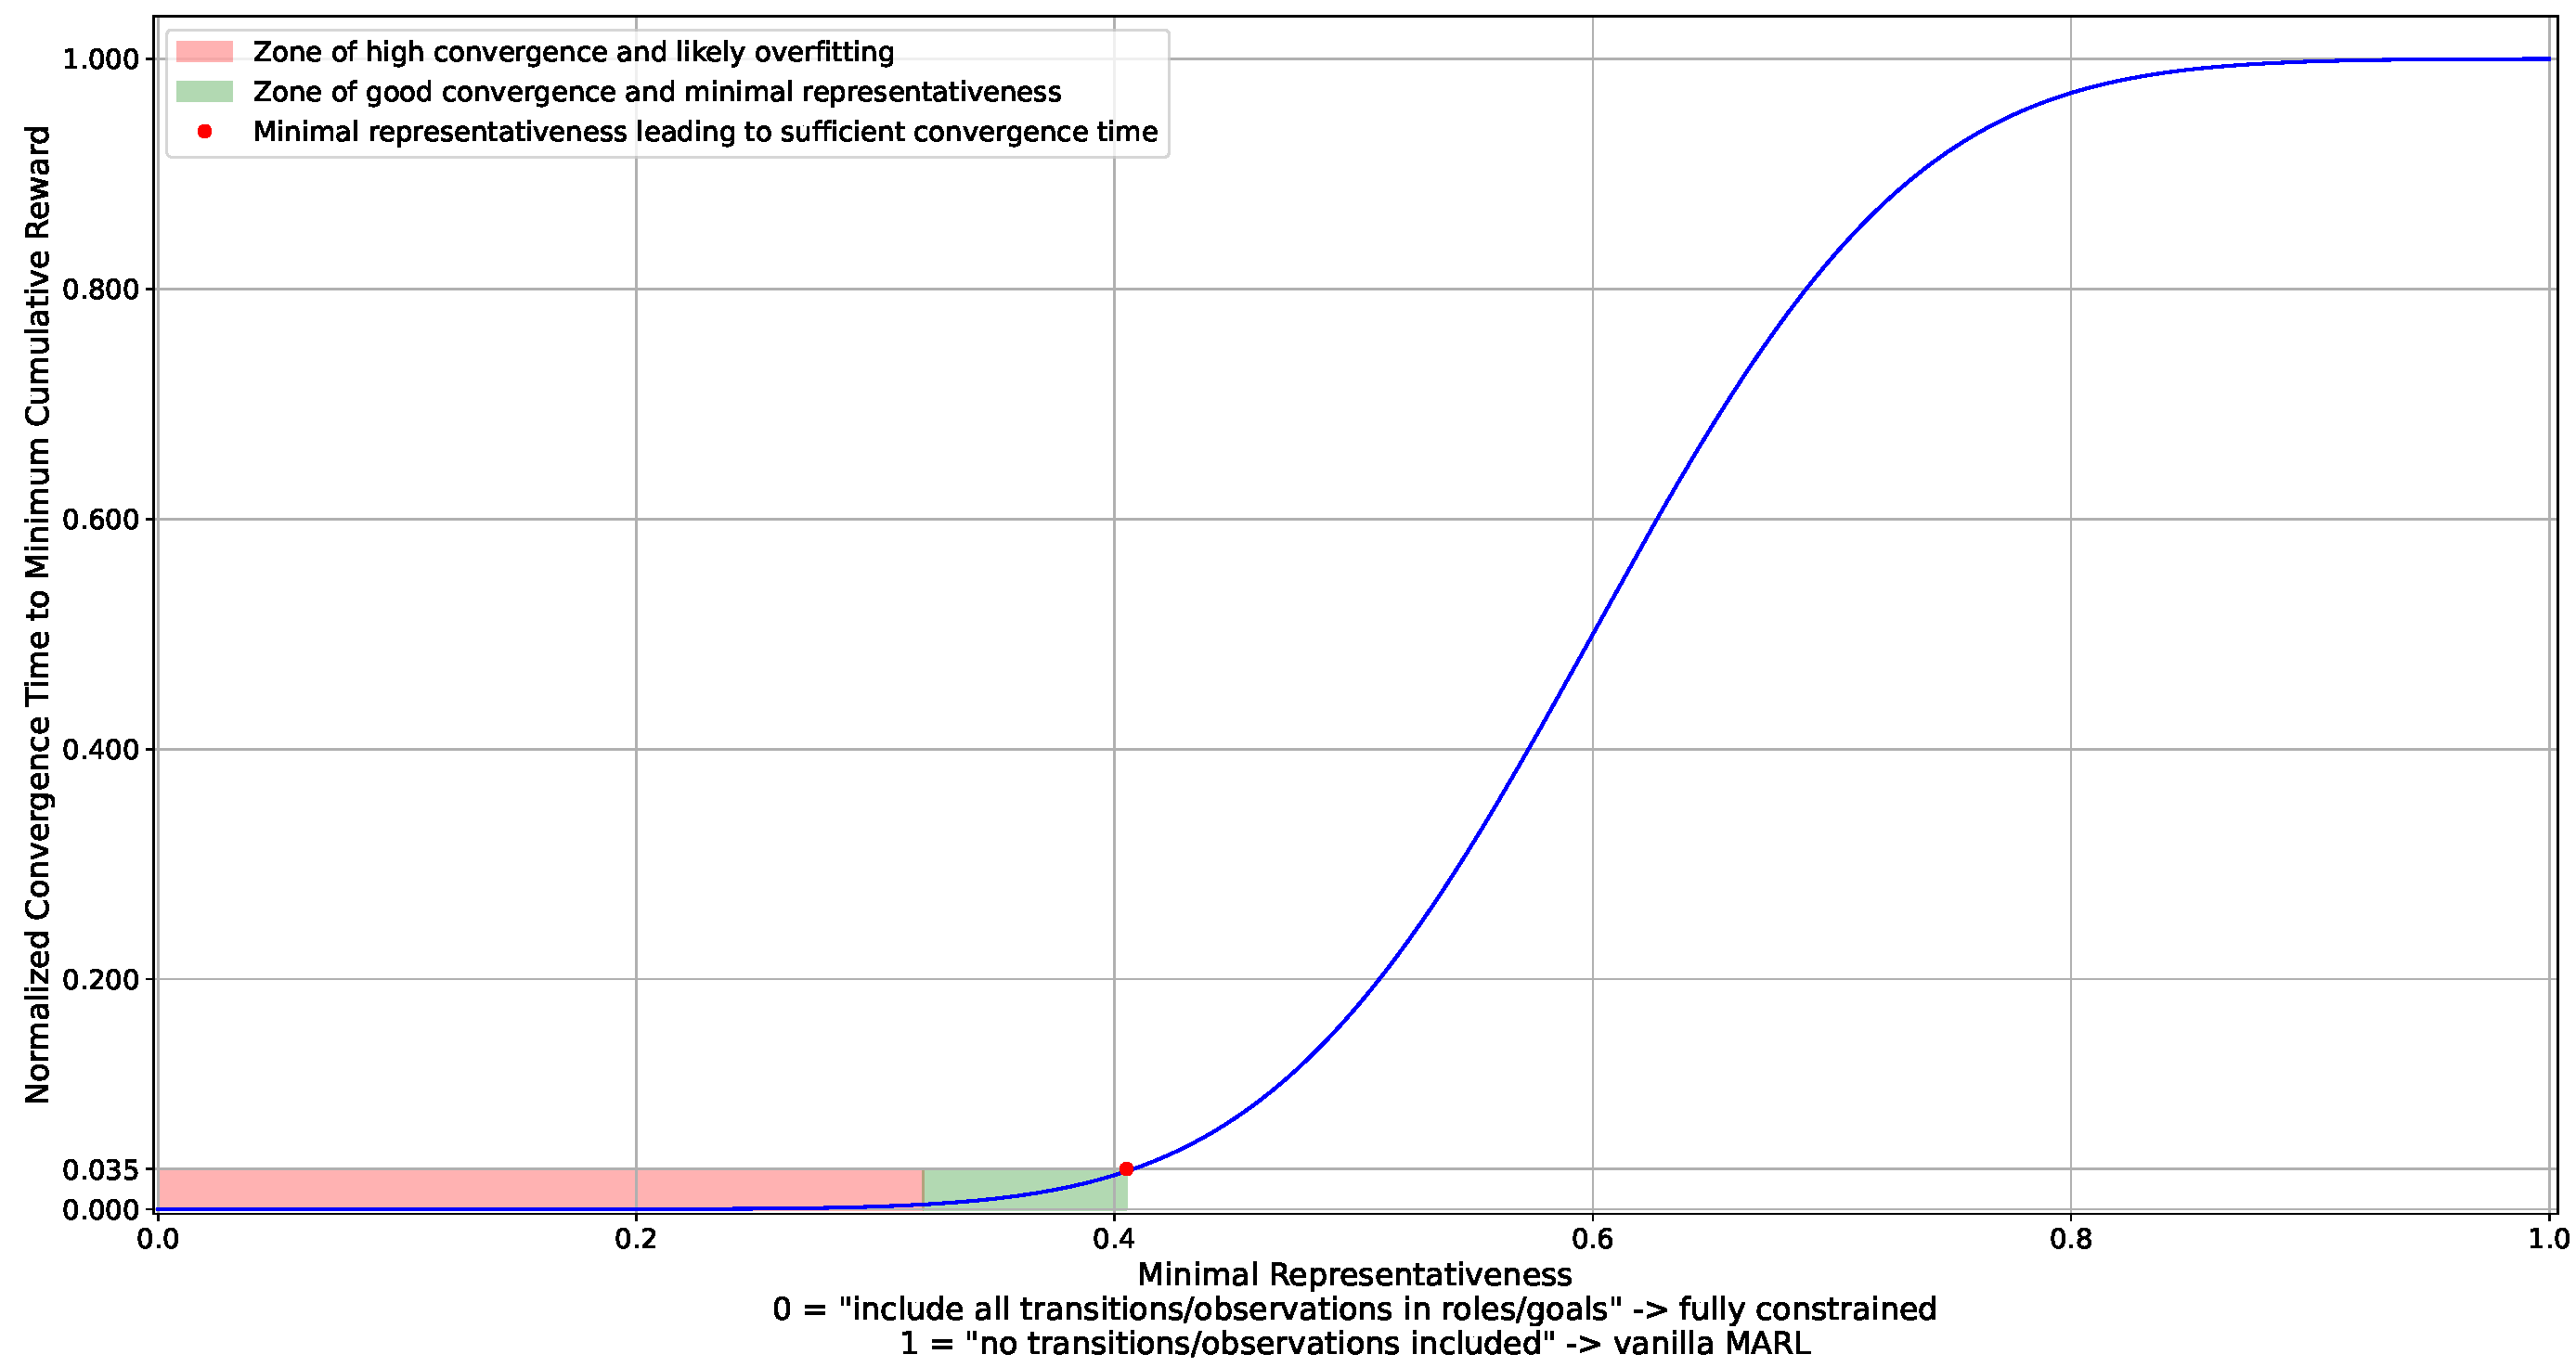
\includegraphics[trim=0cm 0cm 0cm 0cm, clip, width=1.\linewidth]{figures/convergence_time_relative_to_representativeness.pdf}
    \caption{Temps de convergence normalisé en fonction de la représentativité minimale}
    \label{fig:conv_time_repr}
\end{figure}

\begin{algorithm}[H]
    \caption{Algorithme de l'activité d'analyse}
    \label{alg:auto_temm}
    \DontPrintSemicolon

    \KwIn{
        Politique conjointe entraînée $\pi^j$ ;
        ODec-POMDP $d_\Omega$ ;
        Spécification initiale $\mathcal{MM}$ ;
        Seuil de convergence normalisé (défaut : 3.5\%) $\eta$
    }

    \KwOut{
    Spécification organisationnelle inférée $\mathcal{MM}_{\text{implicit}}$ ;
    Score de fit organisationnel $\text{OF}$
    }

    \tcp*[l]{1. Collecte des trajectoires}
    Générer les historiques individuels $\mathcal{D}_{\text{trans}}$ depuis $d_\Omega$ sous $\pi^j$ \;
    $\mathcal{D}_{\text{obs}} \gets$ trajectoires d'observations individuelles issues de $\mathcal{D}_{\text{full}}$ \;

    \tcp*[l]{2. HPO sur distance et seuil de clustering}
    \For{$t \in \{obs, trans\}$}{
        \ForEach{métrique de distance $\delta_t$}{
            \ForEach{seuil minimal de cluster $\tau_t$}{
                Appliquer clustering avec $(\delta_t, \tau_t)$ \;
                Calculer $\sigma_{\text{obs}}, \sigma_{\text{trans}}, N_{\text{clusters}}$ \;
                Score $\gets \alpha (\sigma_{\text{obs}} + \sigma_{\text{trans}}) + \beta N_{\text{clusters}}$ \tcp*[l]{par défaut : $\alpha=0.4$, $\beta=0.6$}
                Retenir $(\delta_t^*, \tau_t^*)$ avec Score minimal \;
            }
        }
    }

    \tcp*[l]{3. Application du clustering avec HPO optimal}
    Clustering des observations : $\mathcal{D}_{\text{obs}} \rightarrow C_{obs}$ via $(\delta_{obs}^*, \tau_{obs}^*)$ \;
    Clustering des transitions : $\mathcal{D}_{\text{trans}} \rightarrow C_{trans}$ via $(\delta_{trans}^*, \tau_{trans}^*)$ \;

    \tcp*[l]{4. HPO sur la représentativité (convergence)}
    \For{$t \in \{obs, trans\}$}{
    \ForEach{représentativité $\rho_t$}{
    Inférer $\mathcal{MM}_{\rho_t}$ à partir des clusters \;
    Initialiser une politique $\pi^j_{\rho_t}$ \;
    Entraîner $\pi^j_{\rho_t}$ sur $(d_\Omega, \mathcal{MM}_{\rho_t})$ jusqu'à atteindre $R_{\min}$ \;
    Enregistrer le temps de convergence $c_{\rho_t}$ tel que $ct_t(\rho_t) = c_{\rho_t}$ \;
    }

    \tcp*[l]{5. Sélectionner le point de coude}
    $\rho_t^* \gets max(\{\rho_t \ | \ ct_t(\rho_t) < \eta \})$ \tcp*[r]{par défaut $\eta = 3.5\%$}
    }

    \tcp*[l]{6. Inférence finale des rôles et objectifs}
    Inférer les rôles à partir de $\mathcal{D}_{\text{trans}}, \delta^*, \tau^*, \rho^*$ \;
    Inférer les objectifs à partir de $\mathcal{D}_{\text{obs}}, \delta^*, \tau^*, \rho^*$ \;

    \tcp*[l]{7. Calcul du fit organisationnel}
    Calculer SOF (structurel) et FOF (fonctionnel) à partir des variances intra-cluster \;
    $\text{OF} \gets \frac{1}{2}(\text{SOF} + \text{FOF})$ \;

    \Return{$\mathcal{MM}_{\text{implicit}}, \text{OF}$}
\end{algorithm}



\chapter{Transférer et superviser en environnement réel}
\label{chap:transferring}

\noindent L'\textbf{activité de transfert} traite les éléments formels suivants :
\[
    \mathcal{D}_{H^j}, \texttt{need\_update} \gets \texttt{transfer}(\pi^j_{\text{latest}}, \mathcal{E}, \mathcal{D}_{H^j})
\]

L'\textit{activité de transfert} a deux objectifs principaux : (1) déployer en continu la politique conjointe la plus récente $\pi^j_{\text{latest}}$ dans l'environnement réel $\mathcal{E}$ afin d'assurer l'action et l'interaction efficaces des agents ; et (2) collecter de nouvelles trajectoires réelles $(\omega^j_t, a^j_t, \omega^j_{t+1})$ pour enrichir l'ensemble de trajectoires $\mathcal{D}_{H^j}$ utilisé pour mettre à jour l'environnement simulé et les spécifications organisationnelles.

À notre connaissance, aucun framework n'offre à la fois un déploiement asynchrone des politiques et une collecte automatique des historiques conjoints, déclenchée par seuil, dans une boucle fermée capable de se synchroniser avec une chaîne d'apprentissage. Cette absence limite fortement l'automatisation du cycle de conception des \acn{SMA} en environnement réel.

\paragraph{Cadre de transfert}

Nous proposons un cadre théorique général mettant en œuvre un système de contrôle asynchrone et événementiel, responsable de l'exécution des politiques et de la collecte des traces. Il maintient un tampon de trajectoires, déclenche la phase de réentraînement lorsqu'un seuil de taille est atteint, et veille à ce que la politique la plus récente soit toujours utilisée. Cette logique de contrôle repose sur deux mécanismes :
(i) une \texttt{Boucle de transfert} (\texttt{Transfer Loop}) pour le déploiement temps réel et la collecte de données, et
(ii) un \texttt{Déclencheur de mise à jour} (\texttt{Update Trigger}) qui lance le processus de conception dès qu'assez de données sont disponibles. Le système empêche les mises à jour parallèles multiples et garantit la synchronisation entre les phases de transfert et de modélisation.

\vspace{-0.3em}
\begin{algorithm}[H]
    \caption{Activité de transfert}
    \label{alg:transferring}
    \DontPrintSemicolon
    \KwIn{Politique actuelle $\pi^j_{\text{latest}}$, environnement réel $\mathcal{E}$, base de trajectoires $\mathcal{D}_{H^j}$}
    \KwOut{Base de trajectoires mise à jour $\mathcal{D}_{H^j}$, signal de mise à jour $\texttt{need\_update}$}

    \vspace{0.3em}
    \SetKwProg{Transfer}{Procédure \normalfont BoucleDeTransfert}{}{}
    \Transfer{}{

    \While{le SMA est actif dans l'environnement $\mathcal{E}$}{
    \tcp*[l]{Exécution de la politique la plus récente}
    $\omega^j_t \gets \texttt{observe}(\mathcal{E})$ \;
    $a^j_t \gets \pi^j_{\text{latest}}(\omega^j_t)$ \;
    $\omega^j_{t+1} \gets \texttt{apply}(\mathcal{E}, a^j_t)$ \;
    Ajouter $(\omega^j_t, a^j_t, \omega^j_{t+1})$ au tampon temporaire $\mathcal{B}$ \;

    \tcp*[l]{Vérification du déclenchement de la mise à jour}
    \If{$|\mathcal{B}| \geq \texttt{batch\_size}$}{
        Ajouter $\mathcal{B}$ à $\mathcal{D}_{H^j}$ et vider $\mathcal{B}$ \;
        $\texttt{need\_update} \gets \texttt{True}$ \;
        \If{$\texttt{running\_update} = \texttt{False}$}{
            \texttt{launch\_update()} \tcp*[r]{Appel asynchrone}
        }
    }
    }
    }
\end{algorithm}

Ce mécanisme garantit (i) la continuité d'exécution, (ii) la réactivité à l'arrivée de nouvelles données, et (iii) l'automatisation des cycles de mise à jour. Il constitue le lien entre le monde simulé et le contexte réel de déploiement en ajustant en continu la boucle de conception à l'évolution de l'environnement, condition essentielle pour l'autonomie à long terme d'un \acn{SMA}.



\chapter*{Conclusion}
\addcontentsline{toc}{chapter}{\textbf{Conclusion}}

\noindent
Cette troisième partie a introduit la méthode \textbf{\acn{MAMAD}} comme une réponse concrète aux limites identifiées dans les approches actuelles de conception de \acn{SMA}. Reposant sur un cycle itératif structuré en quatre phases — \textit{Modélisation}, \textit{Apprentissage}, \textit{Analyse}, \textit{Transfert} —, \acn{MAMAD} articule de manière cohérente des outils symboliques (spécifications organisationnelles) et \acn{MARL} pour guider la conception, l'entraînement et l'adaptation d'agents intelligents dans des environnements complexes.

\medskip

\noindent
La méthode s'appuie notamment :
\begin{itemize}
    \item sur une modélisation fidèle des environnements à partir de données empiriques,
    \item sur un entraînement contraint par des spécifications organisationnelles intégrées au sein du cadre \textit{MOISE+MARL},
    \item sur une analyse des trajectoires pour inférer les structures émergentes de l'organisation apprise,
    \item et enfin sur un transfert contrôlé permettant l'amélioration itérative du \acn{SMA}.
\end{itemize}

\noindent
Dans la partie suivante, nous proposons de valider expérimentalement cette méthode à travers son implémentation concrète dans un outil dédié, \acn{CybMASDE}, et son application à plusieurs environnements représentatifs. L'objectif est de démontrer la capacité de \acn{MAMAD} à produire automatiquement des \acn{SMA} performants, explicables et conformes à des exigences organisationnelles dans des contextes variés.

\medskip

\noindent
Nous évaluons notamment la méthode selon des critères d'efficacité, d'automatisation, de conformité aux contraintes et d'explicabilité, tout en comparant ses résultats à ceux d'approches classiques non guidées par des modèles organisationnels.

\bigskip

La \autoref{part:experimentation} met donc à l'épreuve la méthode \acn{MAMAD}, en analysant ses performances et sa pertinence au regard des verrous identifiés sur différents scénarios.
